
%%%%%%%%%%%%%%%%%%%%%%%%%%%%%%%%%%%%%%%%%
%%            LMU-Vorlage              %%
%%                                     %%
%%         zur Erstellung einer        %%
%%   Dissertation mit pdflatex/latex   %%
%%                                     %%
%%  (2002) Robert Dahlke               %%
%%         & Sigmund Stintzing         %%
%%%%%%%%%%%%%%%%%%%%%%%%%%%%%%%%%%%%%%%%%

\documentclass[12pt]{book}

%%%%%%%%%%%%%%%%%%%%%%%%%%%%
%%   Zusaetzliche Pakete  %%
%%%%%%%%%%%%%%%%%%%%%%%%%%%%

\usepackage{a4wide}
\usepackage{fancyhdr}
\usepackage{graphicx}
\usepackage[bookmarks]{hyperref}
\usepackage{graphicx}
\usepackage{natbib}
\usepackage{rotating}
\usepackage[caption = false]{subfig}
\usepackage{dcolumn}
\usepackage{amsmath,amsfonts, amssymb}
\usepackage{txfonts}
\usepackage[export]{adjustbox}
\usepackage{newtxtext,newtxmath}
\usepackage[Bjornstrup]{fncychap}
%\usepackage{tgheros}
%\usepackage{fontspec}
%\setmainfont{Garamond}
%\setmonofont{Garamond}
%\setsansfont{Garamond}

% important commands
\providecommand{\s}[1]{\text{#1}}
\providecommand{\ion}[2]{\textup{#1\,\textsc{\lowercase{#2}}}}
\providecommand{\lya}[0]{Ly$\alpha$}
\providecommand{\lam}[0]{\lambda}
\providecommand{\e}[1]{\times 10^{#1}}
\providecommand{\mc}[1]{\multicolumn{1}{c}{#1}}

\newcommand{\ang}{\mbox{\normalfont\AA }}
\newcommand{\ditto}[1][.4pt]{\xrfill{#1}~~\textquotedbl~~\xrfill{#1}}
\newcommand{\pkg}[1]{\textup{\textsc{#1}}}

\newcommand*\sun{\ensuremath{\odot}}
\newcommand*\degr{\ensuremath{^\circ}}
\newcommand*\arcmin{\ensuremath{^\prime}}
\newcommand*\arcsec{\ensuremath{^{\prime\prime}}}
\renewcommand{\familydefault}{\sfdefault}

% Journal abbreviations
\newcommand\mnras{MNRAS}           	% MNRAS
\newcommand\araa{ARA\&A}            	% Annual Review of Astronomy and Astrophysics
\newcommand\apj{ApJ}                		% Astrophysical Journal
\newcommand\apjl{ApJ}                		% Astrophysical Journal, Letters
\newcommand\nat{Nature}              		% Nature
\newcommand\aap{A\&A}                		% Astronomy and Astrophysics
\newcommand\aj{AJ}                   			% Astronomical Journal (the)
\newcommand\apjs{ApJS}               		% Astrophysical Journal, Supplement
\newcommand*\rmxaa{Rev. Mexicana Astron. Astrofis.}
\newcommand*\na{New A}
\newcommand\aapr{A\&ARv}             % Astronomy and Astrophysics Review (the)
\newcommand\pasp{PASP}
\newcommand\pasa{Publ. Astron. Soc. Australia}
\newcommand\aaps{AAPS}
\newcommand\memras{MmRAS}
\newcommand\procspie{Proc.~SPIE}
\newcommand\nar{New~Astron.~Rev.}
\newcommand\baas{BAAS}    

%%%%%%%%%%%%%%%%%%%%%%%%%%%%%%
%% Definition der Kopfzeile %%
%%%%%%%%%%%%%%%%%%%%%%%%%%%%%%
\pagestyle{fancyplain}
\renewcommand{\chaptermark}[1]%
         {\markboth{\thechapter.\ #1}{}}
\renewcommand{\sectionmark}[1]%
         {\markright{\thesection\ #1}}
\lhead[\fancyplain{}{\bfseries\thepage}]%
    {\fancyplain{}{\bfseries\rightmark}}
\rhead[\fancyplain{}{\bfseries\leftmark}]%
    {\fancyplain{}{\bfseries\thepage}}
\cfoot{}

\usepackage{hyperref}
\hypersetup {
pdfpagemode = {UseNone},
pdftitle = {The kinematic nature of baryons in the multi-phase circumgalactic media of high-redshift radio galaxies},
pdfauthor = {Sthabile Kolwa},
pdflang = {de-DE}
} 

%%%%%%%%%%%%%%%%%%%%%%%%%%%%%%%%%%%%%%%%%%%%%%%%%%%%%
%%  Definition des Deckblattes und der Titelseite  %%
%%%%%%%%%%%%%%%%%%%%%%%%%%%%%%%%%%%%%%%%%%%%%%%%%%%%%

\newcommand{\LMUTitle}[9]{
  \thispagestyle{empty}
  \vspace*{\stretch{1}}
  {\parindent0cm
   \rule{\linewidth}{.7ex}}
  \begin{flushright}

    \vspace*{\stretch{1}}
    \sffamily\bfseries\Huge
    #1\\
    \vspace*{\stretch{1}}
    \sffamily\bfseries\large
    #2
    \vspace*{\stretch{1}}
  \end{flushright}
  \rule{\linewidth}{.7ex}
  \vspace*{\stretch{5}}
  \begin{center}
    
\includegraphics[width=2in]{siegel}
  \end{center}
  \vspace*{\stretch{1}}
  \begin{center}\sffamily\LARGE{#5}\end{center}
  \newpage
  \thispagestyle{empty}

  \cleardoublepage
  \thispagestyle{empty}

  \vspace*{\stretch{1}}
  {\parindent0cm
  \rule{\linewidth}{.7ex}}
  \begin{flushright}
    \vspace*{\stretch{1}}
    \sffamily\bfseries\Huge
    #1\\
    \vspace*{\stretch{1}}
    \sffamily\bfseries\large
    #2
    \vspace*{\stretch{1}}
  \end{flushright}
  \rule{\linewidth}{.7ex}

  \vspace*{\stretch{3}}
  \begin{center}
    \Large Dissertation\\
    \Large an der #4\\
    \Large der Ludwig--Maximilians--Universit\"at\\
    \Large M\"unchen\\
    \vspace*{\stretch{1}}
    \Large vorgelegt von\\
    \Large #2\\
    \Large aus #3\\
    \vspace*{\stretch{2}}
    \Large M\"unchen, den #6
  \end{center}

  \newpage
  \thispagestyle{empty}

  \vspace*{\stretch{1}}

  \begin{flushleft}
    \large Erstgutachter:  #7 \\[1mm]
    \large Zweitgutachter: #8 \\[1mm]
    \large Tag der m\"undlichen Pr\"ufung: #9\\
  \end{flushleft}

  \cleardoublepage
}


%%%%%%%%%%%%%%%%%%%%%%%%%%%%
%%  Beginn des Dokuments  %%
%%%%%%%%%%%%%%%%%%%%%%%%%%%%

\begin{document}

  \frontmatter


  \LMUTitle
      {The kinematic nature of baryons in the multi-phase circumgalactic media of high-redshift radio galaxies}               				% Titel der Arbeit
      {Sthabile Kolwa}                       				% Vor- und Nachname des Autors
      {Johannesburg, S\"udafrika}           	% Geburtsort des Autors
      {Fakult\"atsname}                         		% Name der Fakultaet
      {M\"unchen 2019}                          		% Ort und Jahr der Erstellung
      {17 Oktober 2019}                            		% Tag der Abgabe
      {Prof Dr Paola Caselli}                        % Name des Erstgutachters
      {Prof Dr Simon White}                        % Name des Zweitgutachters
      {28 November 2019}                         						% Datum der muendlichen Pruefung


  \tableofcontents
  \markboth{Table of Contents}{Table of Contents}
 
  \listoffigures
  \markboth{List of Figures}{List of Figures}

  \listoftables
  \markboth{List of Tables}{List of Tables}
  \cleardoublepage
  
 \phantomsection
  \addcontentsline{toc}{chapter}{\protect Zusammenfassung}
\markboth{Zusammenfassung}{Zusammenfassung}
 
\chapter*{Zusammenfassung}
Die Wechselwirkung zwischen dem zentralen Schwarzen Loch einer Galaxie und den Baryonen (Gas, Staub und Sterne) innerhalb der galaktischen Scheibe hat einen entscheidenden Einfluss auf die Entwicklung der Galaxie. In dieser Arbeit soll der Einfluss von Akkretion eines Schwarzen Lochs auf die Aktivit\"at des aktiven galaktischen Kerns (AGN) demonstriert werden. Zuerst wird durch einen statistischen Test zwischen den 1.4 GHz Leuchtst\"arken und den pseudo-3D Dichtemessungen von 2716 Radio AGN, welche mit dem Karl G. Jansky Very Large Array (JVLA) beobachtet wurden, mit $z\lesssim0.8$ gezeigt, dass die Leuchtkraft eines kosmischen Jet und die Galaxienanzahldichte der Umgebung weitestgehend unkorreliert sind. Stattdessen ist es wahrscheinlicher, dass interne Prozesse, wie etwa die Akkretion von kaltem Gas auf einen AGN, eine weitaus wichtigere Rolle als Regulator der AGN Aktivit\"at spielen. Als Zweites werden Linien mit Ruhewellenl\"angen im UV Bereich, gemessen im Zentrum der $z=2.92$ Radiogalaxie MRC 0943-242 mit dem Very Large Telescope (VLT) Integralfeldspektrograph MUSE (Multi-unit Spectroscopic Explorer), dazu benutzt, die Emissions- und Absorptionskoeffizienten des ionisierten Gas von Gaswolken in der n\"aheren Umgebung der Galaxie zu bestimmen. Die Beobachtung von blauverschobenen Emissionslinien relativ zur systematischen Geschwindigkeit der Galaxie weist auf Radiojetgetriebene Gasausstr\"omungen hin. Absorptionslinien suggerieren, dass sich eine gro\ss skalige ($r\,\gtrsim\,60$\,kpc), mit Metallen angereicherte H\"ulle von absorbierendem Gas jenseits der Bugsto\ss welle des Radiojets befindet. Die Position dieses absorbierenden Materials suggeriert, dass es durch eine fr\"uhzeitig einsetzende AGN R\"uckkopplung gebildet wurde. Abschlie\ss end wird ein Pilotprojekt pr\"asentiert, welches die mit ALMA (Atacama Large Milimeter-submilimeter Array) f\"ur sieben Galaxien mit hoher Rotverschiebung (HzRGs, $z\gtrsim2.9$) gemessene [C\,\textsc{i}](1-0) Feinstrukturlinie als Indikator f\"ur molekuklares Gas nutzt. Die [C\,\textsc{i}](1-0) Linie wird alternativ oft als Indikator f\"ur molekularen Wasserstoff (H$_2$) mit niedriger Metallizit\"at und Dichte genutzt. Das Ergebnis dieses Studie zeigt, dass f\"ur sechs der sieben HzRGs die [C\,\textsc{i}](1-0) Feinstrukturlinie nicht gemessen werden konnte. F\"ur die Galaxie TN\,J0121+1320 mit $z=3.52$ konnte die [C\,\textsc{i}](1-0) Linie jedoch mit einer Halbwertsbreite von $\approx160$\,km\,s$^{-1}$, verbreitert durch AGN Jet-getriebene Turbulenzen des molekularen Gases im interstellaren Mediums (ISM), nachgewiesen werden. Eine blinde Suche nach [C\,\textsc{i}](1-0) in der Umgebung der Galaxien resultiert in engen Linien mit einer Halbwertsbreite zwischen 20 -- 100\,km\,s$^{-1}$ in einem projezierten Abstand $d\geq10$\,kpc vom galaktischen Zentrum, indikativ f\"ur kinematisch ruhiges molekulares Gas im zirkumgalaktischen Medium (CGM). Das Fehlen von H$_2$ Gas in sechs von sieben Galaxien bedeutet, dass fast der gesamte Vorrat an molekularem Gas schon durch fr\"uhere Phasen rascher Sternentstehung aufgebraucht wurde. Diese Studien zeigen, dass die Akkretion von Material auf Schwarze L\"ocher und die Energieabgabe von Radio-Jets eine hohe Bedeutung f\"ur die Kinematik und Morphologie des Gases im ISM und CGM von Ragiogalaxien haben.
  
  \cleardoublepage
   \phantomsection
  \addcontentsline{toc}{chapter}{\protect Abstract}
\markboth{Abstract}{Abstract}

\chapter*{Abstract}

The interaction between a galaxy's central black-hole and the baryons (gas, dust and stars) within the host galaxy's disk plays a crucial role in influencing a galaxy's evolution. In this work, the influence of black-hole accretion on active galactic nucleus (AGN) activity is demonstrated. This is {\it initially} done using a statistical test between the 1.4 GHz luminosities, and pseudo-3D density measures of 2716 radio AGN detected by the Karl G. Jansky Very Large Array (JVLA) at $z \lesssim 0.8,$ which shows that the jet power of the AGN, traced by the radio luminosities, and the galaxy number density are largely uncorrelated. Rather, secular processes in the form of cold gas accretion onto the AGN are likely to play a more important role in regulating AGN activity. {\it Secondly,} by fitting the rest-frame ultraviolet (UV) spectral lines detected by the Very Large Telescope (VLT) integral field unit spectrograph MUSE (Multi-unit Spectroscopic Explorer), we obtain detections of the nuclear region of the $z=2.92$ radio galaxy, MRC 0943-242. On the line and continuum spectra extracted from this region, we parametrise the properties of gas within the galaxy halo in terms of its line absorption and emission. By fitting the emission lines, we obtain evidence of gas blueshifted up to $\sim$1000 km s$^{-1}$ relative to the galaxy's systemic velocity, suggesting radio jet-driven bulk outflows of gas. The absorption-line fits indicate the presence of a large-scale ($r \gtrsim 60$ kpc), metal-enriched shell of absorbing gas located beyond the bow-shock of the radio jets. 
The location of this absorber suggests that it was formed by an early AGN feedback event. {\it Finally,} we present a pilot study of molecular gas traced by [\ion{C}{i}](1-0) detected with ALMA (Atacama Large Milimeter-submilimeter Array) in seven high-redshift radio galaxies (HzRGs) at $z \gtrsim 2.9.$ The [\ion{C}{i}](1-0) fine-structure line is often used as an alternative probe for molecular hydrogen, H$_2,$ under low gas density and metallicity conditions. The results show that six of the seven HzRGs in the sample have non-detections of [\ion{C}{i}](1-0). The galaxy TN J0121+1320 at $z=3.52,$ however, has a clear [\ion{C}{i}](1-0) detection of line-width of $\rm FWHM\simeq160$ km s$^{-1}$ broadened by AGN jet-driven turbulence of molecular gas within the interstellar medium (ISM). A blind search for [\ion{C}{i}](1-0) in the field surrounding the galaxies results in detections at projected distances $d \gtrsim 10$ kpc from the hosts which have line-widths of $\rm FWHM = 20 - 100$ km s$^{-1}$ indicative of kinematically quiet molecular gas in the circumgalactic medium (CGM). The fact that H$_2$ gas is not traced in six of the host galaxies in the sample implies that large reservoirs of molecular gas in the host galaxy ISMs were consumed through earlier phases of star-formation. These studies demonstrate the sheer importance of the black-hole-powered AGN and radio jets in altering the kinematics and morphology of gas within the ISM and CGM of a radio galaxy. 

  \mainmatter\setcounter{page}{1}
  \chapter{Introduction}

% -------------------------------------------------------------------------------------
%           												Section 1.1
% -------------------------------------------------------------------------------------
\section{Feedback Mechanisms in Radio Galaxies}

A plethora of evidence now exists in support of the notion that the central supermassive black-hole of a galaxy can have a significant impact on the evolution of the galaxy hosting it. In particular, the well-constrained empirical relation between the central black-hole mass ($M_\bullet$) and the stellar velocity dispersion ($\sigma$) of a galaxy is evidence of this \citep{kormendy2013}. This $M_\bullet$-$\sigma$ relation is important in establishing the importance of the black-hole, a relatively small-scale object at the centre of a galaxy, to the larger distribution of baryons (stars, gas, and dust) surrounding it.

The central black-hole, when it is sufficiently massive, can have a dramatic impact on the dynamic and thermal state of baryons in a galaxy; in other words, when its mass ($M_\bullet$) is well above a threshold of approximately $M_\bullet \gtrsim 10^8 - 10^9~\rm M_\odot.$ In this case, the centre of a galaxy is referred to as an active galactic nucleus (AGN). The influence that the AGN has on the physics of the baryons within and around the galaxy are described as AGN feedback mechanisms. They impact the evolution of a galaxy through large expulsions of energy approximately equivalent to the black-hole rest energy ($E_\bullet$), $E_\bullet = \epsilon M_\bullet \rm{c}^2,$ where $\epsilon$ is the efficiency of the energy output and, c, the light-speed. This energy output can alter the availability of molecular gas reservoirs from which stars form in a galaxy and as a result impede or accentuate the growth of a galaxy depending on the effect. 

In negative feedback, the AGN accelerates bulk outflow of gas which can result in star-formation within a galaxy slowing down or coming to a halt. The energy output of the AGN, whether radiative or kinetic, may also enhance the star-formation rate through shock-driven collapse of giant molecular clouds -- an example of positive feedback. 

The types of galaxies looked at, in this work, are radio galaxies in which AGN feedback operates in the form of powerful energy injections that can affect the thermodynamics, kinematics, morphology, ionisation state, and displacement of gravitationally bound gas within the interstellar and circumgalactic mediums (ISMs and CGMs). The rate of mass accretion onto the central black-hole determines the rate of mechanical energy output which is measured by the total luminosity of the AGN ($L_{\rm AGN}$). Furthermore, the first time derivative of the rest-mass equation shows that the mass accretion rate onto the AGN ($\dot{M}_{\rm acc}$) is proportional to $L_{\rm AGN}$ such that $L_{\rm AGN} = \epsilon \dot{M}_{\rm acc} c^2$ for an efficiency of $\epsilon.$

Within and surrounding Within radio galaxies, AGN feedback operates through the mechanical power of the radio jets that are produced by non-thermal, synchrotron radiation from the accretion disk surrounding the black-hole. This is the kinetic-mode of feedback and is radiatively inefficient unlike the radiative-mode whereby the energy output occurs in the form of radiation (or photon winds) as its name suggests. AGN feedback is thus bimodal \citep{heckman2014}. Since jet outflows that occur in radio galaxies are responsible for the kinetic-mode of feedback, studying radio AGN is key to obtaining a better understanding of how this type of feedback operates. In fact, kinetic feedback has been studied in great detail in galaxies at low redshifts ($z \lesssim 1$) and consequently nearby radio galaxies are often considered evolutionary analogues to radio galaxies at higher redshifts. 

In this thesis, I use a statistical study of the influence of environment density and radio luminosity to determine whether low redshift ($z \leq 0.8$) sources in groups are more likely to host powerful radio AGN. We also study the environments of radio galaxies in the high-redshift Universe by observing the multi-phase gas of a sample of seven radio galaxies at $z \gtrsim 2.9,$ with the aim of determining the impact of their powerful radio jets on their ISM and CGMs. Through these observations, it is possible to determine the effect of radio jets on the ionised, molecular and neutral phases of the gas. This is crucial to understanding the ways in which kinetic-mode feedback can alter the evolution of a galaxy \citep{Fabian2012}. Observing this in high redshift radio galaxies (HzRGs), in particular, can help unlock the mystery behind AGN feedback as it occurs in the early Universe 1 to 3 Gyr after the Big Bang. 

% -------------------------------------------------------------------------------------
%           												Section 1.2
% -------------------------------------------------------------------------------------
\section{The Birth of Radio Astronomy}\label{section:early-radio-surveys}
Radio astronomy began with the development of the first radio telescopes and surveys which led to our present understanding of radio galaxies. Many note that radio astronomy started with a serendipitous discovery made by an employee of Bell Telephone Labs, New Jersey in the U.S. While investigating the effect of thunderstorms on transcontinental communication, Karl Guthe Jansky's radio receiver detected a static hiss that appeared to originate from the same location in the sky every 24 hours. The signal would be detected once every sidereal day (four minutes prior to the end of the solar day) which led Jansky to postulate that the signal, detected at a frequency of $\nu_{\rm obs} = 20.5$ MHz ($\lambda_{\rm obs} = 14.6$m), was not terrestrial in origin. This discovery led him to publish a report based on the finding entitled {\it Electrical Disturbances Apparently of Extraterrestrial Origin} - arguably one of the most important radio astronomy publications to date \citep{Jansky1933b,Jansky1933a}.

In 1937, Grote Reber, a radio engineer and also an avid fan of Jansky went on to construct a 9.5 m paraboloid antenna radio receiver sensitive to $\nu_{\rm obs} = 160$ MHz ($\lambda_{\rm obs} = 1.9$m) radiation which was capable of detecting radio signals from the nucleus of the Milky Way, Sagittarius A* \citep{Reber1940}. Other discoveries that followed in the wake of these observations were that of the famous supernova remnants Cassiopeia A, Puppis A and the radio galaxy, Cygnus A. In 1944, Reber completed perhaps the first ever radio survey, the results of which are shown in Fig. \ref{fig:Reber-map-sky-1944} \citep{Reber1944}. 

\begin{figure}[!ht]
     \centering
     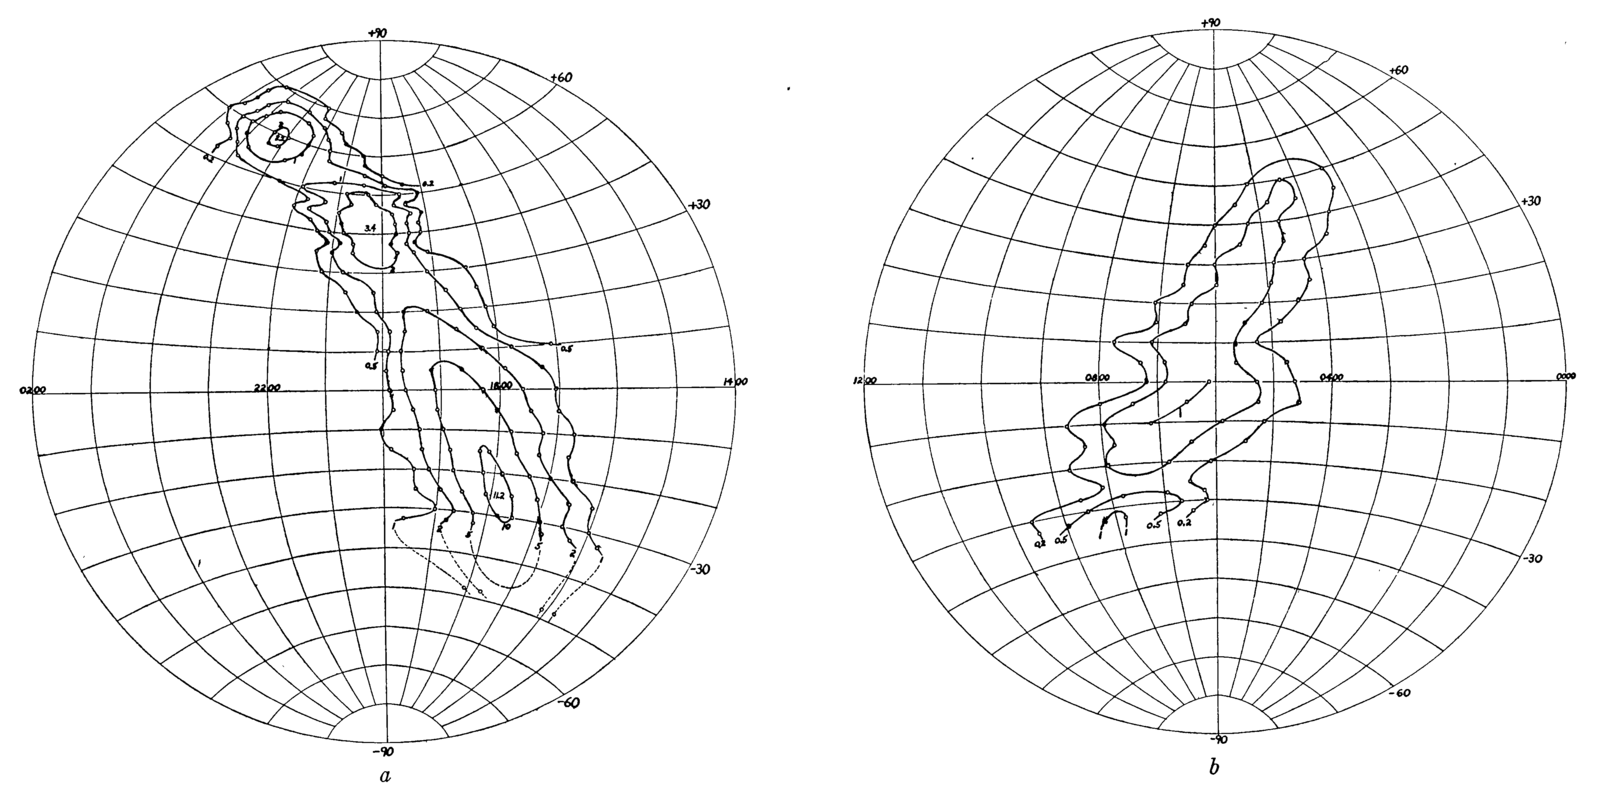
\includegraphics[width=0.8\textwidth]{plots_chp1/Reber_radiomap_1944.png}
     \caption[160 MHz radio map from \citet{Reber1944}]{Intensity contour lines of $\nu_{\rm obs} = 160$ MHz radio emission mapped out by Grote Reber on the self-built 9.5 m paraboloid radio telescope \citep{Reber1944}.}
     \label{fig:Reber-map-sky-1944}
\end{figure}

Both Jansky's discovery and Reber's work were fundamental in introducing the use of radio frequencies in detecting distant objects both within the Milky Way and beyond it. Techniques used in astronomy were developed further through the enhancement of radio receiver technologies used during World War II which led to Baade and Minkowski's own discoveries at the Palomar Observatory, Mount Wilson whose observations showed that two of the sources Reber's first survey detected, Cassiopeia A and Puppis A, spatially coincide with diffuse optical emission referred to as `nebulosities' which were also seen to have large velocity dispersions. Furthermore, the disturbed optical morphology of Cygnus A revealed evidence of it being involved in a galaxy merger \citep{BaadeMinkowski1954}. These cross identifications of a radio sources with optical emission proved that the bright, discrete radio signals picked up by radio surveys were not merely `radio stars' but rather galaxies much like the Milky Way that were emitting powerful bursts of radio emission. Consequently, the term `radio galaxy' was introduced into the astronomy lexicon. 

In order for a radio source to be considered a radio galaxy, an optical counterpart is required due to the fact that redshifts are computed from rest-frame optical, ultraviolet (UV) or near-infrared (near-IR) spectra. Hence, measuring the Doppler shifts of spectral lines at these wavelengths is the primary method for obtaining galaxy redshifts or luminosity distances. Distance is also required to convert the projected sizes of observed components in a galaxy e.g. the extent of the radio lobes (radio sizes) into physical sizes and flux densities into luminosities \citep{Moffet1966}. Once their distances were estimated, radio galaxies became known as the most distant galaxies observable \citep{Stern1999}. 

\section{Motivation}\label{section:motivation}
% M-sigma relation - black-hole and galaxy co-evolution
The empirical $M$-$\sigma$ relation, introduced in section 1.1, states that the mass of the central black-hole ($M_\bullet$) of a galaxy is proportional to its velocity dispersion. This implies that radio galaxies, which generally have high stellar masses, also host very massive central black-holes. They also have high bolometric luminosities ($L_{\rm bol}$) luminosities due to $L_{\rm bol}$ increasing proportionally with the accretion rate as well as the central black-hole mass. 

Based on this, it is rather apparent then that radio galaxies are good places to begin tracing evidence of the kinetic-mode of feedback that occurs within galaxies. There are several other reasons why these particular galaxies are crucial to our understanding of galaxy evolution. 

For one, they provide an opportunity to test theories in cosmology given their detection during redshift epochs that probe the very distant and early Universe at $z\sim4-6$ \citep{LillyLongair1984,Miley1989,Lacy1994a,
Waddington1999,VanBreugel1999,Jarvis2009,Saxena2018}. Their detection up to these high redshifts is essential because by $z\sim6,$ the majority of neutral hydrogen that existed in the Universe during the so-called `Dark Ages' has already been ionised through radiation emitted by the first galaxies and quasars. This early period, referred to as the Epoch of Reionisation (EoR), begins some 150 Myr after the Big Bang (at a redshift of $z\sim11$ and continues up to a cosmic time of 1 Gyr ($z\sim6$) \citep{Zaroubi2013}. Thus, the detection of radio galaxies at high redshifts make them good cosmological probes for parametrising the physics of galaxy formation in the early Universe \citep{Fan2006,Banados2018}.  

% How do galaxies grow / aggregate their mass?
Radio galaxies also allow us to gain better insight into how galaxies aggregate their mass through star-formation in their formative phases. The brightness of stellar emission from galaxies can be determined from optical and near-infrared band magnitudes \citep{GunnOke1975}. In particular, the relation between the brightness of flux measured in the $K$-band (central wavelength: $\lambda_{\rm c}=2.2~\mu$m) which traces redshifted ultraviolet (UV) and optical emission from young stars and redshift show the evolution of flux from stellar emission with cosmic time. This observed relation is known as the Hubble $K$-$z$ diagram (e.g. Fig. \ref{fig:K-z-Lilly1984}). Granted that $K$-band magnitudes are detectable at redshifts of up to $z<4,$ the empirical $K$-$z$ relation for ensembles of radio sources can be used to test cosmology and galaxy evolution models  \citep{LillyLongair1984,EalesRawlings1996,Eales1997}. More recently, the work of \citet{Inskip2002} showed that the $K$-$z$ relation for a sample of radio galaxies fits reasonably to an Einstein-de Sitter cosmology model for a matter density ($\Omega_{\rm M}$) and dark energy density ($\Omega_\Lambda$) of ($\Omega_{\rm M}=1, \Omega_\Lambda=0$). Despite $\Omega_\Lambda=0$ being ruled out by better constraints of cosmological parameters by \citet{Planck2016} measurements from the cosmic microwave background (CMB), these studies still display the potential usefulness of the $K$-$z$ diagram to cosmology.  

\begin{figure}[!ht]
    \centering
    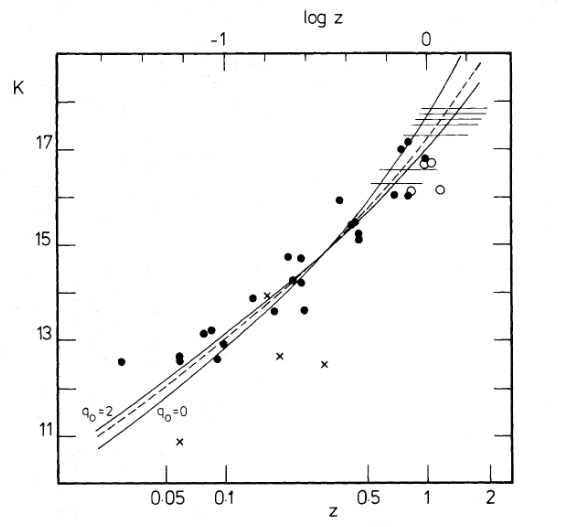
\includegraphics[width=0.8\textwidth]{plots_chp1/K_z_Lill1982.png}
    \caption[Near-infrared Hubble $K$-$z$ diagram \citep{LillyLongair1982}]{Infrared Hubble $K$-$z$ relation from \citet{LillyLongair1982} and is shown for cosmological deceleration parameters $q_0=0$ and $q_0=2$ against the observed magnitudes.}
    \label{fig:K-z-Lilly1984}
\end{figure}

% fix this paragraph ....
The $K$-$z$ diagram has become a widely used diagnostic for placing constraints on galaxy evolution models given its low level of scatter. The work of \citet{rocca-volmerange2004} makes use of the $K$-$z$ diagram to predict the stellar masses of radio galaxies, in this work. Results indicate that the apparent (observed) $K$-band of the ensemble of radio galaxies originally compiled by \citet{debreuck2002a} and first detected in the Third and Sixth Cambridge Catalogues of Radio Sources (3CR and 6CE) discussed later in section \ref{section:early-radio-surveys}. The galaxies are detected over the redshift range $0 \leq z \leq 4$ and shown against galaxy evolution models which predict the baryon masses of elliptical galaxies (see Fig. \ref{fig:K-z-rocca-volmerange2004-pegase}). For the radio galaxies, the results show that their baryon masses ($M_{\rm bary}$) lie within the range, $10^{11} < M_{\rm bary}/\rm{M}_\odot < 10^{11.5}$ and have an upper limit of $M_{\rm bary}/\rm{M}_\odot < 10^{12}$ imposed on all galaxy types. 

\begin{figure}[!ht]
  \centering
  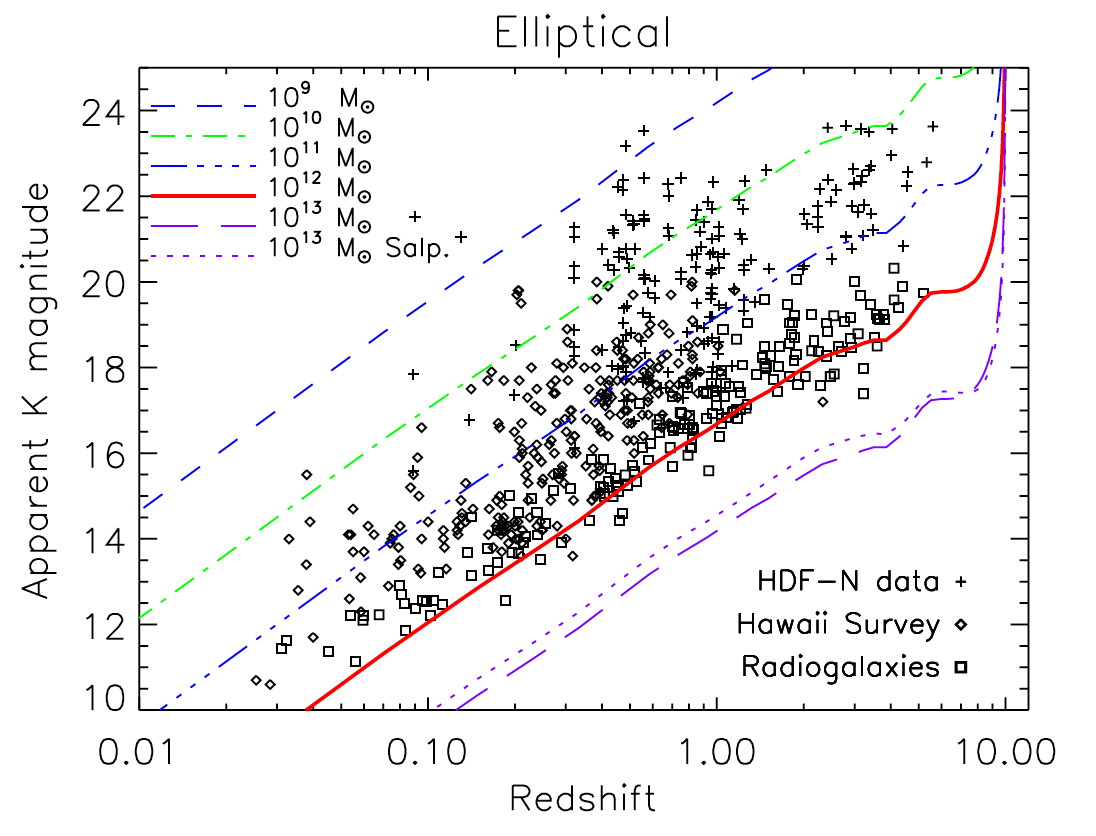
\includegraphics[width=0.8\textwidth]{plots_chp1/K_z_Rocca-Volmerange_2004_pegase.png}
  \caption[$K$-$z$ diagram for elliptical radio galaxies from \citet{rocca-volmerange2004}]{The $K$-$z$ diagrams of radio galaxies (squares) from 3CR and 6CE. The data also includes $K$-band magnitudes of field galaxies from the Hawaii Survey \citep{Songaila1994} (diamonds) and HDF-N \citep[Hubble Deep Field-North;][]{Dickinson2003} (crosses). The initial mass function (IMF) models from \citet{RanaBasu1992} which are given for a range of baryon masses from $M_{\rm bary} = 10^9 - 10^{13}$ M$_\odot.$ A top-heavy (TH) IMF model for $M_{\rm bary} = 10^{13}$ M$_\odot$ is included for comparison.}
  \label{fig:K-z-rocca-volmerange2004-pegase}
\end{figure}

The predicted range of radio galaxy baryon masses from \citet{rocca-volmerange2004} are in agreement with those obtained by \citet{seymour2007} who make use of data from the {\it Spitzer Space Telescope} (SST) \citep{Werner2004}. Datasets comprising SST near-IR photometry for 69 radio galaxies between redshifts of $1.0 < z < 5.2.$ The {\it Spitzer} photometry obtained by the instruments on board the telescope namely the Infrared Array Camera (IRAC; $3.6-8.0~\mu$m), Infrared Spectrograph (IRS; 16 $\mu$m) and Multi-band Imaging Photometer (MIPS; $24-160~\mu$m). Spectral energy distribution (SED) models that aimed to disentangle the stellar, dust and AGN components within the optical and near-IR emission were fit to the IR data. The stellar masses were obtained from $H$-band magnitudes (at a central wavelength of $\lambda_{\rm c} = 1.65$ $\mu$m)\footnote{The choice to use $H$- rather than $K$-band magnitudes is motivated by galaxy evolution models which show that the predicted flux of radio galaxies peaks at the central wavelength of the $H-$band. Additionally, SED-fitting in \citet{Drouart2012} showed that the $H-$band is optimal for sampling the stellar mass without the SED being too contaminated by emission from heated dust.}. The result of this study shows that the radio galaxies have stellar masses (M$_*$) within the range of $10^{11} < M_* < 10^{11.5}$ M$_\odot.$  Radio galaxies, therefore, give us insight into what drives the formation and evolution of galaxies at the high stellar mass end.

% How are jets formed?
Observations of radio galaxies provide us an incredible wealth of information concerning the physical processes that occur within radio galaxies. Although they provide a real-world view of astrophysical objects as they existed, with the caveat of observational biases included, they only provide snapshots of the object at a given epoch. A simulation, although controlled by man instead of nature, provides us with a continuous and evolving view of a galaxy. Hydrodynamical simulations have provided a simulated view of radio jets and the impact they bear on the surrounding gas medium through which they propagate. This has been done by \citet{krause2002} and \citet{krause2005} who demonstrate that shells of neutral hydrogen gas are responsible for absorption troughs observed in hydrogen Lyman-alpha line (\ion{H}{i} Ly$\alpha$) at $1215.67~\text{\AA}$ in the spectra of high redshift radio galaxies (HzRGs). The neutral hydrogen (\ion{H}{i}) gas shells that scatter and absorb Ly$\alpha$ photons can form at the bow shock fronts of radio jets through shock-driven compression of gas. Given sufficient time (over Gyr time-scales), \ion{H}{i} gas shells disintegrate at the shock front of the jets as a result of Rayleigh-Taylor instabilities in the gas medium. 

Another example of simulations which demonstrate the effect of jets on ISM gas are those of \citet{Gaibler2011}. These Monte Carlo 3D simulations depict the propagation of radio jets into a clumpy interstellar medium (ISM). The passage of the radio jets and their impact on the surrounding ISM is shown in time snapshots that illustrate the impact of radio jets on the surrounding gas medium at three different moments during the duty cycle of the radio jet (see Fig. \ref{fig:jet-ism-Gaibler2011}). 

The average duty cycle of radio jet activity persists over a time-scale of $\tau_{\rm jet} \simeq 10 - 100$ Myr. Simulations of jet-gas interactions indeed suggest that radio galaxies are prime targets to study when seeking to understand the impact that radio jets have on ISM gas that lies in proximity to the AGN in radio galaxies.

\begin{figure}[!ht]
  \centering
  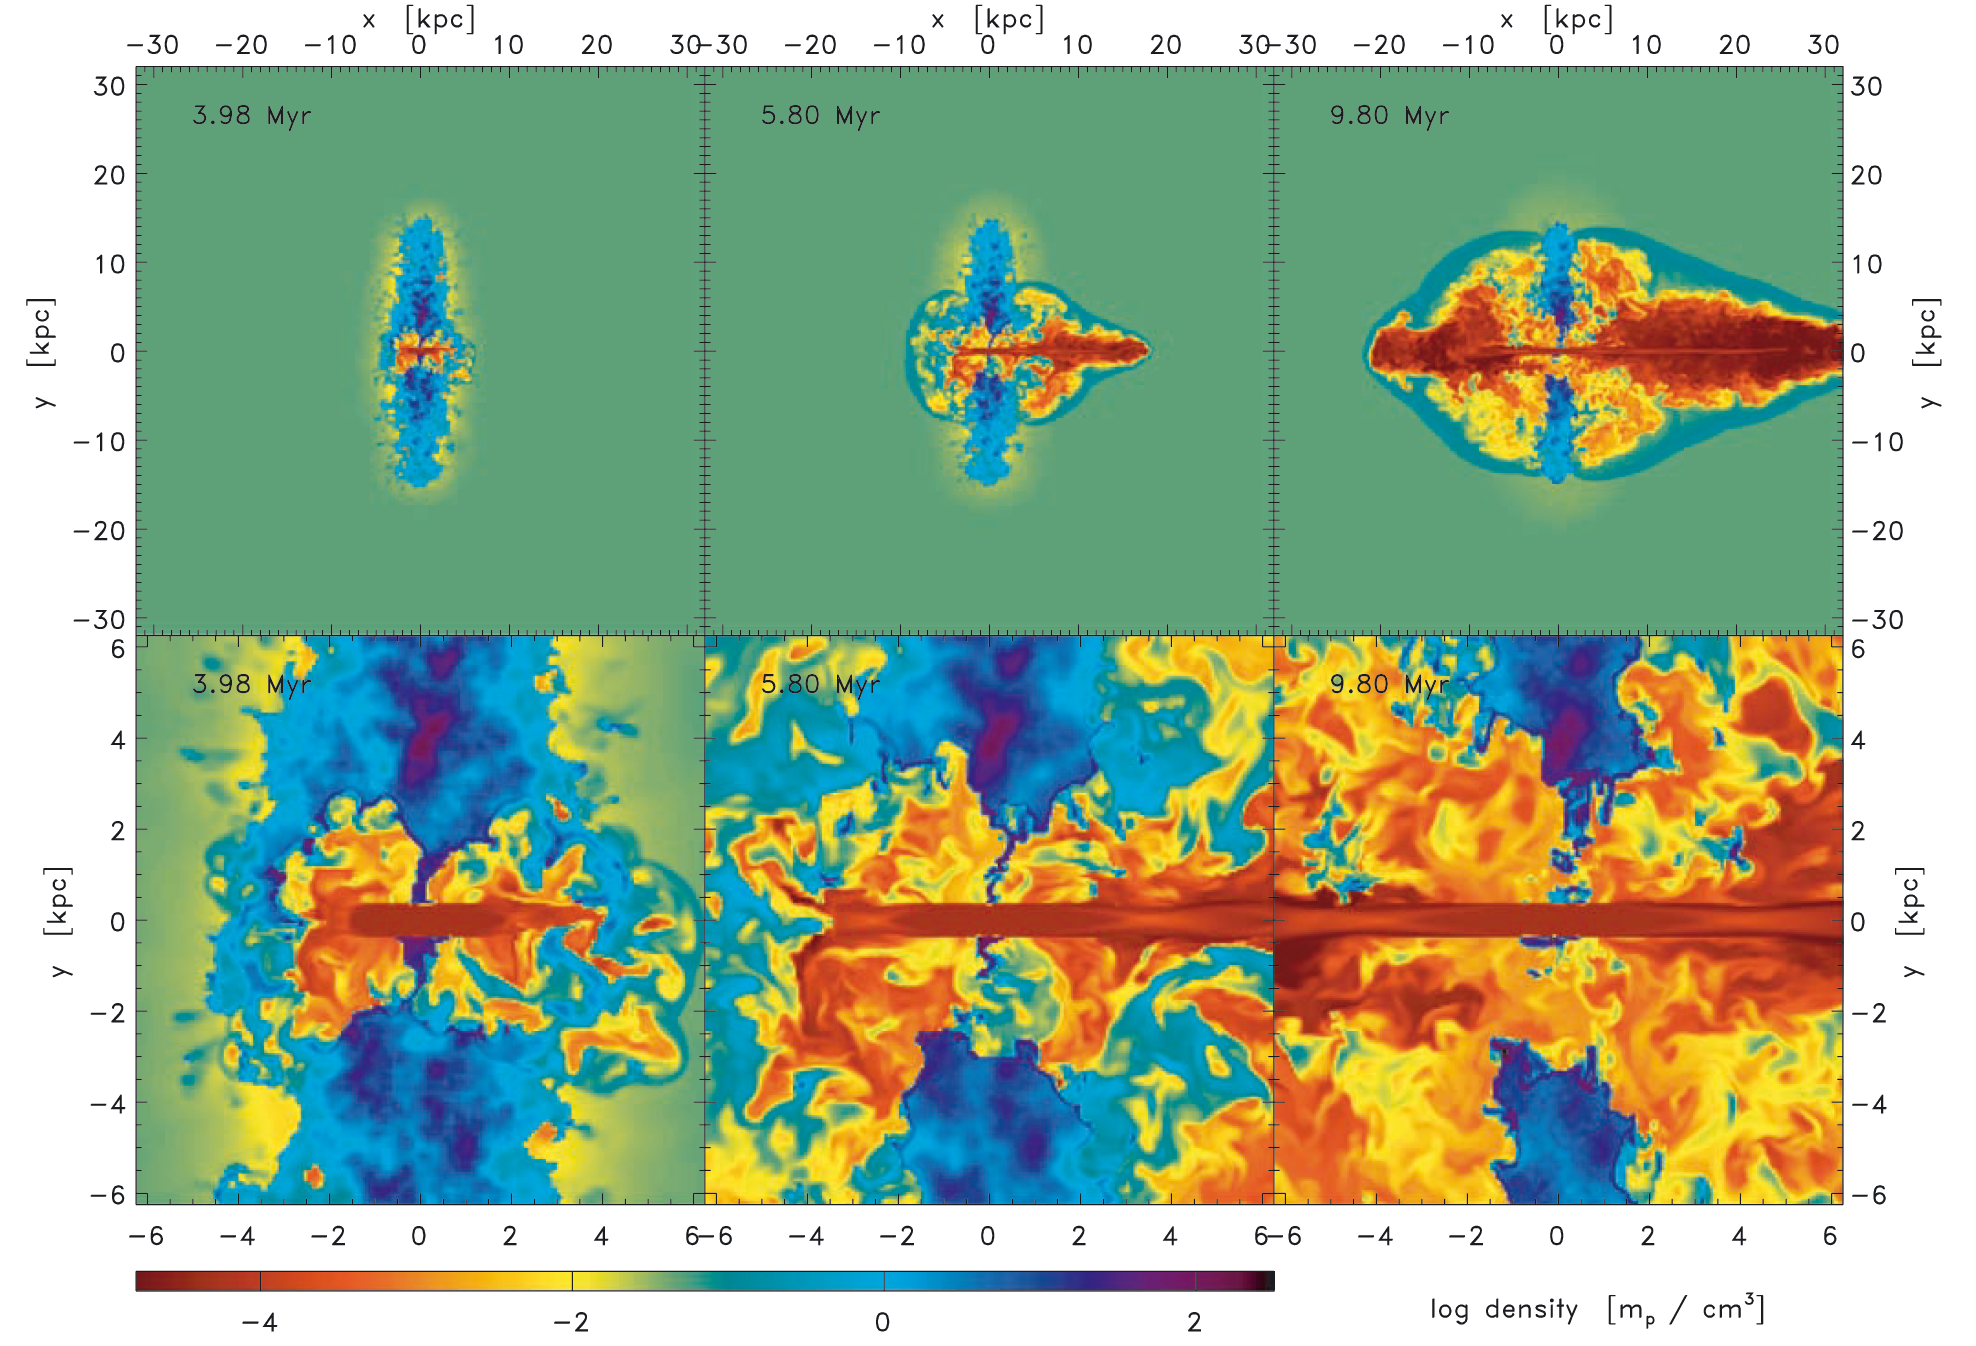
\includegraphics[width=\textwidth]{plots_chp1/jet_gas_sims_Gaibler_2011.png}
  \caption[Simulation snapshots of bi-conical radio jet from \citet{Gaibler2011}]{Snaphots of 3D Monte Carlo simulations of a bi-conical radio jet pummelling through a disc-shaped clumpy interstellar medium with log-normal density distribution in \citet{Gaibler2011}. The growing radio jet begins to plough through the clumpy ISM medium at $t=3.98$ Myr. At $t=5.80$ Myr, an asymmetry in the lobes formed by the relativistic jets has already formed. After $t=9.8$ Myr has passed (the average duty cycle of a radio AGN), extended asymmetric radio lobes enclosed in a bow-shock region are apparent. The upper panel shows a large-scale view of the simulation with the lower panel providing a closer view of the core activity.}
  \label{fig:jet-ism-Gaibler2011}
\end{figure}

%% How could kinetic-mode of feedback affect SF ? 
Radio galaxies at high redshifts are known to form stars rapidly with star-formation rates (SFR) of $\rm SFR \gtrsim 100 - 1000$ M$_\odot \rm yr^{-1}$ inferred from SED fitting to near-IR photometry \citep{Drouart2014,falkendal2019}. The resulting SFR and black-hole accretion rates inferred from the SED-fitting are plotted in Figs \ref{fig:SFR_AGN_LIR-Drouart} and \ref{fig:SFR_AGN_LIR-Falkendal}. Additionally, the Main Sequence of star-forming galaxies which defines the expected SFR for a galaxy of given stellar-mass, is included in the discussion in order to determine how ``normal'' HzRGs are. This normalcy is quantified by the galaxy's shift in relation to the Main Sequence i.e. $\Delta$(M.S.). 

This comparison has been done by \citet{falkendal2019} whose HzRGs sample is shown against the Main Sequences of star-forming galaxies in Fig. \ref{fig:HzRGs-MS-Falkendal2019}. What is clear from these plots, is that at $z > 3,$ more of the HzRGs have slightly lower SFR than is expected for their stellar masses. This implies that, although HzRGs form stars rapidly, they appear to be in a process of quenching. At later epochs, $ 1.3 < z < 3,$ the HzRGs have SFR and $M_*$ that are more consistent with the Main Sequence. Therefore, HzRGs are likely to have undergone earlier phases of rapid star-formation that has begun to slow down by $z\sim3.$ This may be due to AGN jet feedback driving outflows of molecular gas that fuels star-formation.

\begin{figure}[!ht]
    \centering
    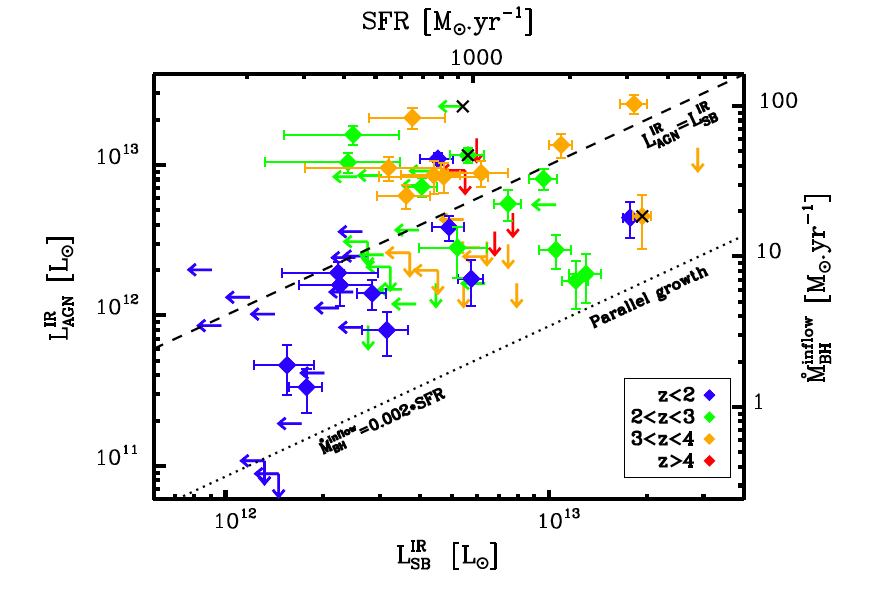
\includegraphics[width=0.95\textwidth]{plots_chp1/SFR_AGN_LIR_Drouart_2014.png}
     \caption[AGN vs SF luminosity from \citet{Drouart2014}]{The total AGN luminosity, $L^{\rm IR}_{\rm AGN}$ as a function of the star-forming luminosity $L^{\rm IR}_{\rm SF}$ from \citet{Drouart2014}. The top axis converts $L^{\rm IR}_{\rm SB}$ to SFR using the \citet{Kennicutt1998} relation. The right axis converts $L^{\rm IR}_{\rm AGN}$ to $\dot{M}_{\rm BH}$ assuming $\epsilon=0.1$ and $\kappa^{\rm Bol}_{\rm AGN}.$ The dashed line marks $L^{\rm IR}_{\rm AGN} = L^{\rm IR}_{\rm SB}.$ This dashed line indicates the relation corresponding to $\dot{M}_{\rm BH} = 0.024 \times \rm SFR,$ using the right and top axes. The dotted line represents the parallel growth mode, where black holes and galaxies grow simultaneously, following the $M_{\rm BH}$-$M_{\rm Gal}$ relation.}
     \label{fig:SFR_AGN_LIR-Drouart}
\end{figure}     
    
\begin{figure}[!ht]
	\centering
    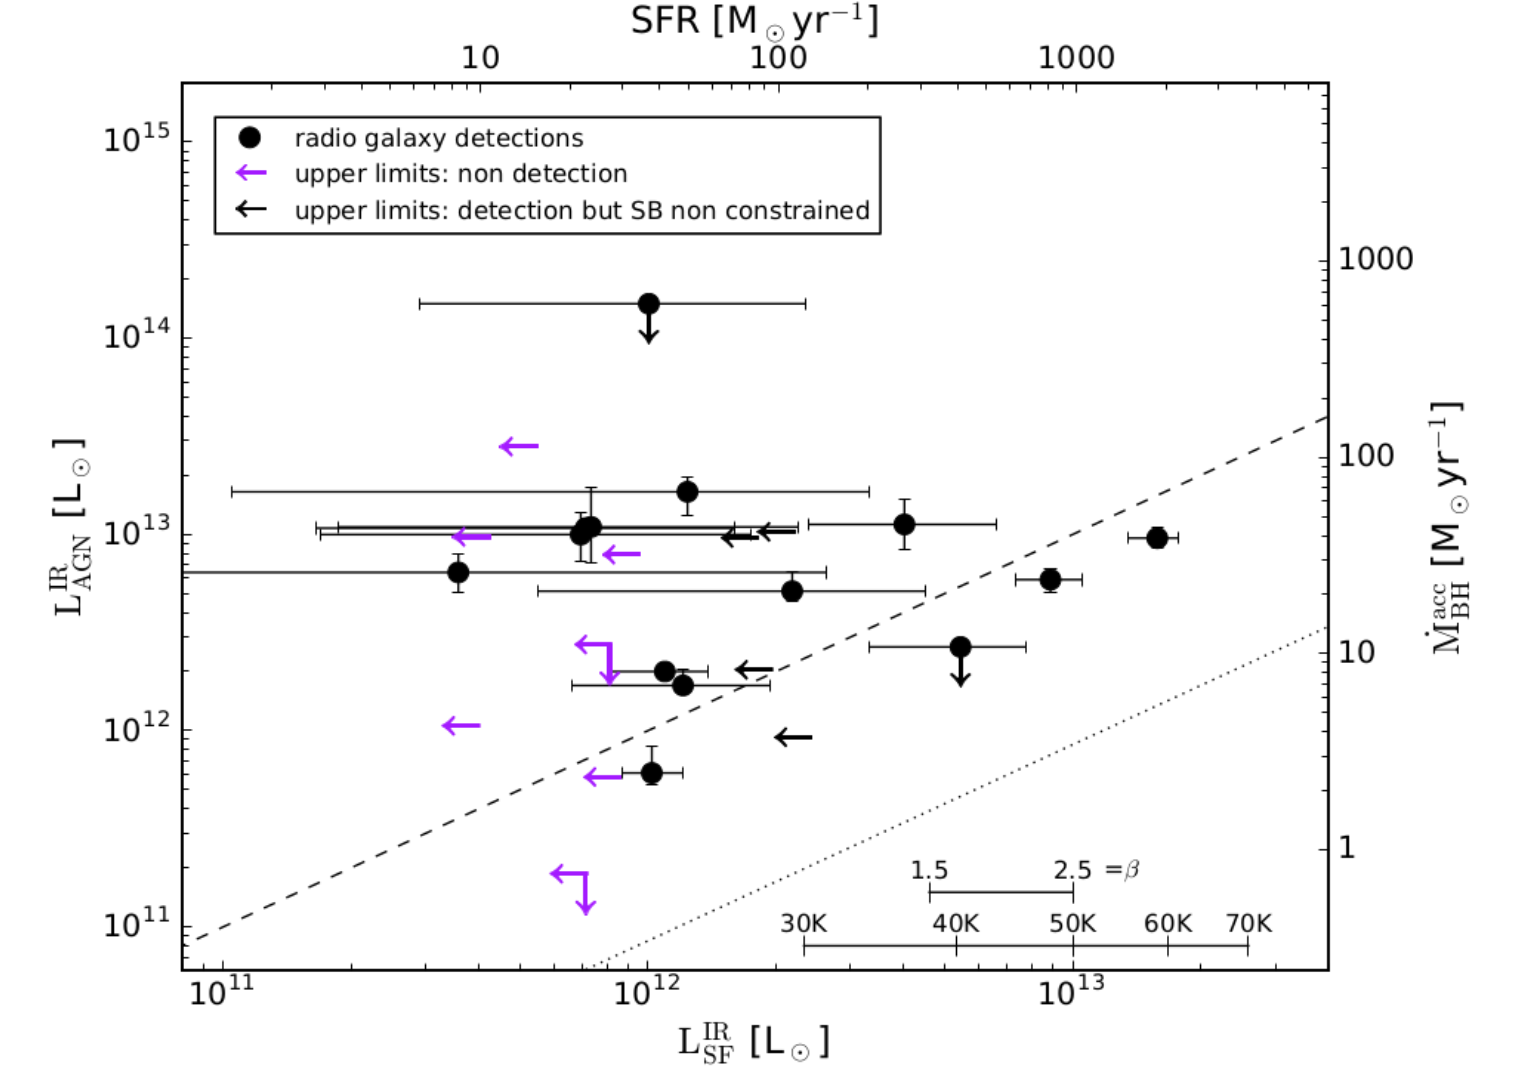
\includegraphics[width=0.8\textwidth]{plots_chp1/SFR_AGN_LIR_Falkendal_2019.png}
    \caption[AGN vs SF luminosity from \citet{falkendal2019}]{$L^{\rm IR}_{\rm AGN}$ as a function of $L^{\rm IR}_{\rm SF}$ from \citet{falkendal2019}. The dashed black line represents equality between the ordinate and abscissa which also represent the star-formation rate (SFR) and black-hole (BH) mass accretion rate ($\dot{M}^{\rm acc}_{\rm BH}$). The dotted shows the axis where black-hole accretion rate $\dot{M}^{\rm acc}_{\rm BH} = 0.002 \times \rm SFR$ which demarcates parallel growth mode where the galaxy and black hole grow in tandem and obey the spheroid mass-BH mass relation.}
    \label{fig:SFR_AGN_LIR-Falkendal}
\end{figure}

\begin{figure}[!ht]
   \centering
   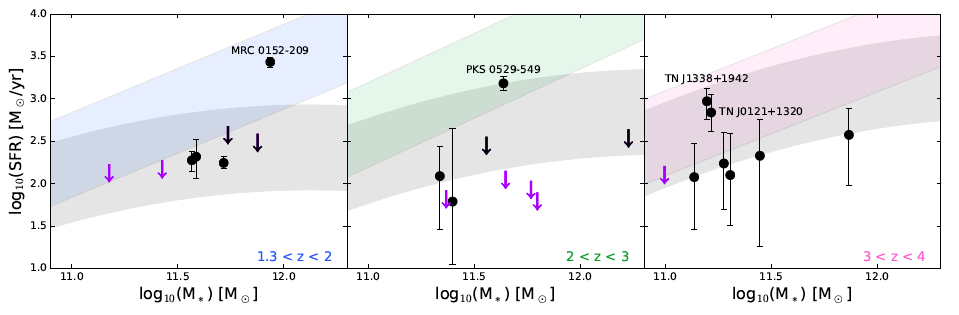
\includegraphics[width=\textwidth]{plots_chp1/HzRGs_main_sequence_Falkendal2019.png}
   \caption[HzRGs relative to Main Sequence in \citet{falkendal2019}]{HzRGs from \citet{falkendal2019} sample are compared to the Main Sequences in the grey shaded regions are taken from \citet{Schreiber2015} while the Main Sequences in colour are those from \citet{Santini2017}.}
   \label{fig:HzRGs-MS-Falkendal2019}
\end{figure}

The Lilly-Madau plot of cosmic star-formation rate density (SFRD) is well known in astronomy and presents an intriguing puzzle that astronomers continue to work on solving \citep{Lilly1995,Madau1996}. The plot shows that at $z \simeq 1.9$ (3.5 Gyr after the Big Bang) the level of cosmic star-formation per epoch per volume reaches a peak as Fig. \ref{fig:SFRD_z_Madau_Dickinson2014} illustrates \citep{MadauDickinson2014}. It is now known that only populations of galaxies that follow the Main Sequence relation can have a significant effect on the cosmic SFRD at $1 < z < 3$ therefore HzRGs, which are found on the main sequence at these redshifts, may be important in explaining why the function, $\psi(z),$ takes on this shape. Unlike normal main-sequence star-forming galaxies which follow the M.S., radio galaxies host powerful jets that have a unique impact on the gas that is gravitationally bound to a galaxy and in close proximity to the AGN. Hence, they hold great importance in providing clues on how star-formation is affected by jet-driven gas outflows. 

\begin{figure}[!ht]
   \centering
   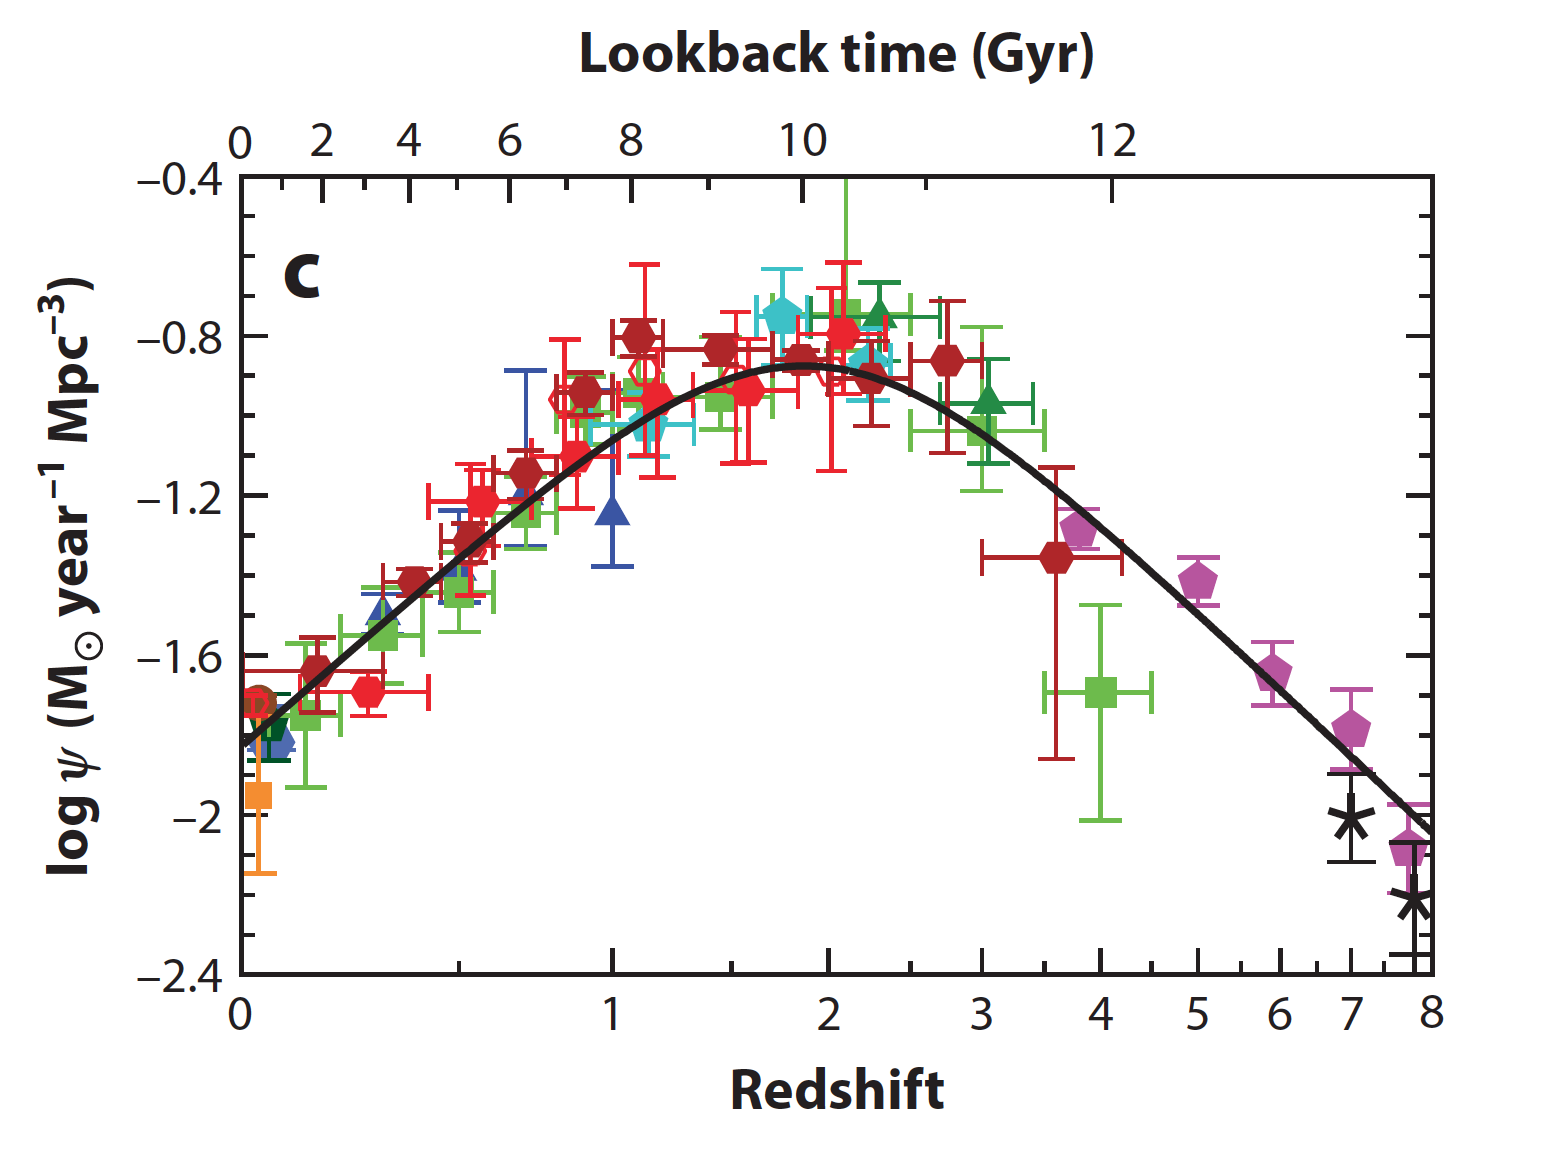
\includegraphics[width=0.8\textwidth]{plots_chp1/SFRD_z_Madau_Dickinson_2014.png}
   \caption[SFRD as a function of redshift in \citet{MadauDickinson2014}]{The star-formation rate density (SFRD) or $\psi(z)$ in M$_\odot$ yr$^{-1}$ Mpc$^{-3}$ given as a function of redshift as well as look-back time in Gyr. The measurements shown are obtained from far ultraviolet (FUV) and near-infrared (NIR) rest-frame luminosities which have been converted to SFR. In the FUV, the equation SFR $= \kappa_{\rm{FUV}} \times L_\nu (\rm{FUV})$ while in the NIR, it is obtained via SFR $= \kappa_{\rm{IR}} \times L_{\rm{IR}}.$}
   \label{fig:SFRD_z_Madau_Dickinson2014}
\end{figure}

\section{Radio Galaxies} 
\subsection{Early radio surveys}
In the wake of Jansky's discovery of cosmic noise, Reber's 160 MHz radio survey and Baade and Minkowsi's identification of radio galaxies, a number of radio surveys were successfully completed. Studies carried out using these surveys' data have resulted in an increase in the number of known radio radio galaxies. 

The Third Cambridge Catalogue \citep[3C;][]{Edge1959} was assembled using the Cambridge Interferometer and is one of first and most prolific radio survey catalogues known. The first and second Cambridge catalogues (1C and 2C) were also compiled in Cambridge during 1950 \citep{Ryle1950} and 1955 \citep{Shakeshaft1955}. Despite being the first Cambridge radio survey catalogues, however, 1C and 2C source detections were affected by astronomical `confusion' - a consequence of more than one astronomical source being detected within one synthesised beam aperture. The result being that several sources are incorrectly resolved as one source. Hence, 3C, which managed to overcome this problem is perhaps the first and most reliable of the Cambridge catalogues to identify a significant number of radio galaxies including 3C 295 which was the most distant radio galaxy known at the time of its discovery \citep{Minkowski1960}. 

The revised 3C Catalogue \citep[3CR;][]{Leslie1961,Bennett1962} observed at $\nu_{\rm obs} = 178$ MHz at a sensitivity or flux limit of $S_{178} = 9$ Jy contained a large number of bright sources at declinations, $\delta > -5^{\circ}$ - in the northern hemisphere. A radio interferometer at the Palomar Observatory Sky Survey \citep[POSS;][]{Veron1966} identified optical counterparts to a number of 3C sources to accurately calibrate the radio source positions and determine whether the optical and radio detections coincide spatially or are related to the same source. More revision of the original 3C source list was carried out by \citet{LaingRileyLongair1983} forming the 3CRR catalogue ($S_{178} \geq 10$ Jy) which contained sources that had yet to be detected due to the flux limitations of the original 3C survey. 

Some of the more notable catalogues that followed were 4C \citep{PilkingtonScott1965} observed at a frequency of $\nu_{\rm obs} = 178$ MHz and a flux limit of $S_{178} = 2$ Jy. This catalogue was crucial in identifying sources that have radio spectral indices ($\alpha$) of $\alpha < -1$ in the flux density-frequency relation $S_\nu \propto \nu^{\alpha}.$ Selecting sources with $\alpha < -1$ led to the identification of sources with small angular sizes and high radio luminosities suggesting that the sources were at significantly greater distances than those with less steep spectra or $\alpha > -1$ \citep{Tielens1979}. The steep spectrum radio sources were added to the 4C Ultra Steep Spectrum Sample \citep[4C/USS;][]{ChambersMiley1990} which consisted of furthest radio galaxies known at the time: 35 of which are at $z > 2$ and 2 at $z > 3.$ The legacy of Cambridge catalogues has continued on through the years leading up to the most recent 10C Survey  \citep{AMIConsortium2011}. 

Another notable radio survey is the Molonglo Reference Catalogue of Radio \citep[MRC;][]{Large1981} which comprises 12,141 sources detected at a tuning frequency of $\nu_{\rm obs} = 408$ MHz at a flux limit of $S_{408} \geq 0.7$ Jy on the Molongolo Radio Telescope \citep{Hunstead1972}. From MRC, steep spectrum sources with $\alpha < -0.9$ were selected at $S_{408} >0.9$ Jy. The steep spectrum sources in this catalogue also have accompanying optical long-slit spectroscopy which identified the majority of the galaxies as having redshifts of $z > 0.8$ \citep{McCarthy1990}. On a subset of the MRC sources with flux densities, $S_{408} >0.95$ Jy and redshifts, $z > 1$ radio galaxies were observed to have extended filaments of optical emission and higher luminosity radio cores and jets than galaxies from the 3C catalogue \citep{McCarthy1991}. 

Many efforts made to build up source catalogues from radio interferometric surveys during the early days of radio astronomy have provided an extensive repository of radio galaxies. This means that we now have a sufficiently wide database from which to study the evolution of radio galaxies from their early formation after the Epoch of Reionisation all the way to the present-day epoch where we observe galaxies in the nearby Universe. 

\subsection{Radio galaxies across cosmic time}
As the large-scale structure of the Universe changes with time as a result of cosmic expansion \citep{Planck2016}, so do the physical properties of galaxies. One of the main goals of this thesis, in fact, is to compare and contrast the properties of radio-loud AGN host galaxies at high and low redshift. In this section, I highlight some the known commonalities and disparities of these galaxies at the different redshift epochs where they are found.  

Radio galaxies are empirically defined as radio-loud sources that have double-lobed morphologies formed through the expulsion of synchrotron radiation from bipolar (bi-directional) jets emitted from their cores. A perfect illustration of this is the nearby galaxy Cygnus A ($z=0.057$), a local radio galaxy first identified by \citet{JennisonDasGupta1953}. Early and more recent interferometric observations shown in Fig. \ref{fig:CygA} exhibit quite nicely its double-lobed radio structure \citep{Moffet1966,CarilliBarthel1996}. Thus, provided that a radio galaxy is at a sufficiently low-redshift for its radio structure to be resolved, its double radio morphology will be apparent. An important cosmological effect makes these morphologies apparent at large distances. It just so happens that at $z > 1,$ the angular diameter distance drops down gradually rather than steeply while the cosmic brightness decreases by a factor of $(1+z)^{-4}.$ This means that the physical sizes of radio lobes do not vary greatly with increasing redshift at $z > 1.$ From radio observations, we know that high-redshift radio galaxies have double-lobe structures that can extend out to $\sim$100 kpc in size and can be resolved even up to $z \lesssim 4$ \citep{Miley1980,carilli1997,pentericci1999}.  

The double-lobe morphologies place them in the category of Fanaroff-Riley II sources which have extended lobes that terminate at edge-brightened hotspots where non-thermal radiation increases in surface-brightness \citep{FanaroffRiley1974}. Their double-lobe morphology also implies that the relativistic jets are oriented along the plane of the sky. Indeed, the orientation of the jets are an important means by which radio sources are classified. A Type 1 radio AGN or quasar has `beamed' jets where the observer looks into the barrel of the ionisation cone. On the other hand, the Type 2 AGN refers to sources with jets that are observed parallel to (or at a small angle from) the plane of the sky. Therefore, by definition, all radio galaxies are Type 2 AGNs. 

Radio galaxies have classically been dichotomised into radio-loud and quiet populations based on their observed radio luminosities. This bi-modality was initially identified in quasar populations. Since radio galaxies are likely to have hidden or dust-obscured quasars at their nuclei, the bi-modal description can be extended to them as well \citep{vernet2001}. 

Generally, radio-loud sources, which are rarer than radio-quiet ones, have comparatively higher radio luminosities and are hosted by elliptical galaxies \citep{Padovani1993} while radio-quiet sources are not \citep{Wilson1995}. Also, the lower limit for radio-loud sources is defined by radio luminosities of $L_{1.4~\rm GHz} \gtrsim 10^{25}$ W Hz$^{-1}$ or $L_{5~\rm GHz} \gtrsim 10^{26}$ W Hz$^{-1}$ \citep{Miller1990}. More recently, radio luminosity functions of sources in the local Universe have shown that the star-forming galaxy populations that do not form jets outnumber AGN by a factors of up to 10 at $L_{1.4~\rm GHz} \lesssim 10^{23}$ W Hz$^{-1}.$ Thus, even though star-forming galaxies may be detectable at radio frequencies, their luminosities tend to be significantly lower than those of radio-loud AGN \citep{Best2005a}. 

The widely accepted theory of jet-formation states that radio jets are formed through synchrotron radiation which is emitted as a result of the acceleration of electrons by magnetic fields. The free electrons are sourced from a plasma surrounding the central black-hole where neutral gas is sufficiently heated and ionised by radiation emitted by the AGN. This so-called synchrotron radiation theory was first proposed by \citet{Shklovskii1953} who stated that synchrotron radiation can power relativistic jets which, over Myr time-scales, form the extended radio lobes with sizes in the order of $\sim$100 kpc. Given that the sources are radio-loud with luminosities detected in radio frequencies of $L > 10^{25}$ W Hz$^{-1}$ and the average lifetime of a radio source (its duty cycle) falls within a range of $\tau \simeq 10-100$ Myr, synchrotron radiation is sufficient to fill radio lobes with energies of up to $E \simeq 10^{60}$ erg assuming an AGN duty cycle of $\tau = 100$ Myr and $L_{\rm AGN} = 10^{46}$ erg. How the radio jets are launched, however, is still largely up for debate.

\begin{figure*}[!ht]
  \centering
  \subfloat[The nearby ($d_{\rm L} = 256.3$ Mpc) radio galaxy, Cygnus A, observed with the Cambridge Telescope with a synthesised beam of $23'' \times 35''$ observed at $\lambda=21$ cm. The corresponding radio contours show the double-lobed morphology. The radio contours are superimposed over an optical image taken using the Hale Reflector Telescope. The optical image has a $4' \times 6'$ wide field-of-view \citep{Moffet1966}.]{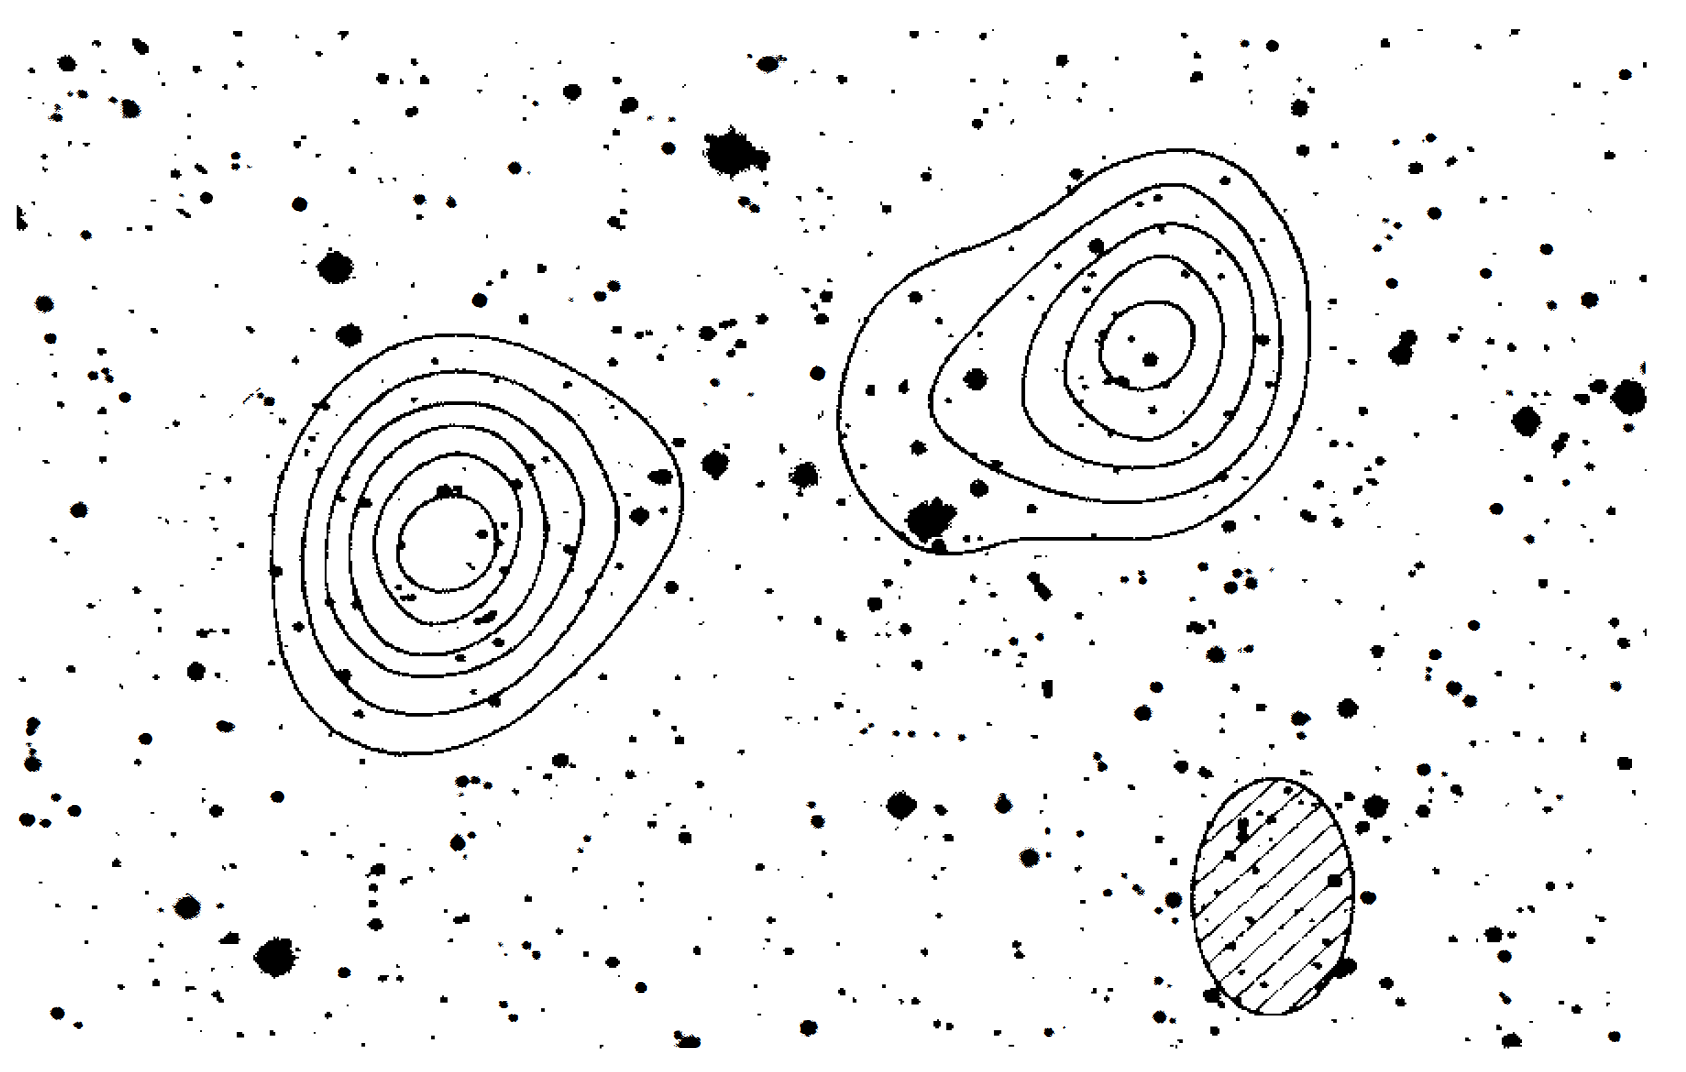
\includegraphics[width=0.9\textwidth]{plots_chp1/Cygnus_A_Hale_Baade_1965.png}}\\
  \subfloat[Cygnus A observed with the Very Large Array (VLA) at tuning frequency of $\nu_{\rm obs} = 5$ GHz \citep{CarilliBarthel1996}.]{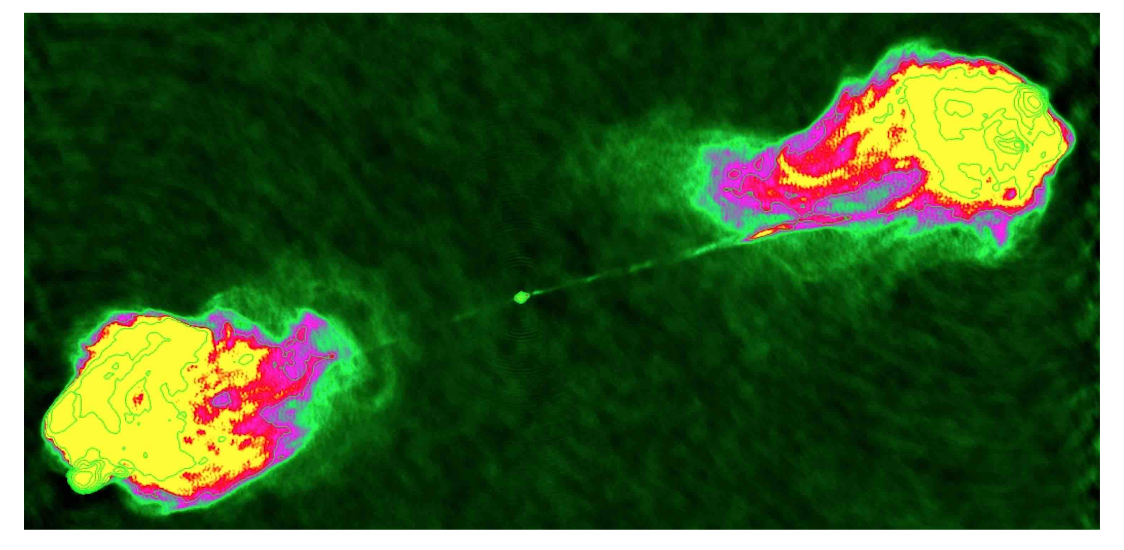
\includegraphics[width=0.9\textwidth]{plots_chp1/CygA_Carilli_Perley.png}}
  \caption[Cygnus A radio imaging in 1966 and 1996]{Radio images of Cygnus A in 1966 and 1996.}
  \label{fig:CygA}
\end{figure*}

The existence of galactic scale magnetic fields is confirmed, furthermore, through the polarisation of light emitted from the AGN. With many observations of polarized emission in radio galaxies having already been carried out by synchrotron radiation has increasingly become a more plausible explanation for the cause of radio jet emission. Radio polarisation studies also show that radio polarisation generally increases with redshift. The degree of polarisation is quantified by the rotation measure (R.M.) defined as,

\begin{equation} 
R.M. = \frac{e^3}{2\pi m_e^2 c^4} \int_0^L n_e(l)B_{||}(l)dl.
\end{equation}

The rotation measure is observed to be stronger at high-redshift than in radio galaxies at $z < 1$  \citep{Saikia1988,Scarrott1990,Tadhunter1992,Jannuzi1991,diSeregoAlighieri1993,
Tran1995,Jannuzi1995,diSeregoAlighieri1996,Jones1996,Feretti1999,Taylor2002,Kaczmarek2018}.
In section \ref{section:early-radio-surveys}, the ultra steep spectrum bias for selecting distant radio galaxies was introduced. Indeed, many studies following the work of \citet{Tielens1979}, who first displayed this bias, have shown that the radio spectral index ($\alpha$) correlates with redshift ($z$). This is referred to as the $\alpha$-$z$ correlation \citep{BlumenthalMiley1979,Chambers1988a,debreuck2002a}. Although a general consensus on the reason for this relation has yet to be reached, several theories have been put forward. 

One theory states that because radio SEDs are generally concave, they appear steeper at higher observed frequencies due to electron energy losses from inverse-Compton scattering. The concave shape also implies that a bias will be introduced at higher redshifts where the rest-frame frequencies detected become higher for a given tuning frequency. However, this idea only holds provided that a radio spectrum is concave which is not always the case \citep{Klamer2006}.  

More recent findings have shown that $\alpha$-$z$ correlation results from a decrease in cosmic microwave background (CMB) energy density with cosmic time. Hence, at earlier epochs the effects of inverse-Compton scattering of CMB photons is stronger resulting in higher electron energy losses at low observed frequencies ($\nu_{\rm obs} \leq 1$ GHz). In combination with selection effects explained in \citet{debreuck2000}, this results in steeper radio spectra at higher redshifts \citep{Morabito2018}.  

The near-infrared $K$-$z$ diagram is introduced as a motivation for studying radio galaxies in section \ref{section:motivation} where $K$-band ($\lambda_{\rm c}=2.2~\mu$m) magnitudes are a proxy for stellar mass because they trace emission from evolved stars. The majority of $K$-$z$ diagrams assembled have shown radio galaxies to have the brightest (lowest) $K$-band magnitudes and therefore the largest stellar masses of $M_*/\rm{M}_\odot \simeq 10^{10} - 10^{12}$ among other galaxy populations \citep{McCarthy1993,jarvis2001,Willott2003,rocca-volmerange2004}. Radio galaxies  having large baryon masses has several implications: according to the principle of downsizing (the more massive structures form at earlier cosmic times) massive galaxies will form stars earlier during their evolution. Secondly, if their black-hole masses are proportional to their stellar masses as the $M_\bullet$-$\sigma$ relation implies, we can expect the AGN to be very luminous and form mechanically powerful radio jets that could disrupt star-formation. 

It has also been mentioned that radio AGN are hosted by elliptical galaxies. Some of the first evidence to emerge for this was in a sample of bright galaxies drawn from the 6C catalogue \citep{Eales1985a,Eales1985b}. JVLA, {\it Hubble Space Telescope (HST)} and near-IR observations of 28 radio galaxies from this sample at $0.6 < z < 1.8$ which show evidence for elliptical galaxy morphologies in {\it HST} imaging. Their optical, near-IR SEDs are also consistent with those of giant elliptical (gE) galaxy populations \citep{Best1997}. Further evidence of $z \sim 1$ radio galaxies being ellipticals is put forward in \citet{McLureDunlop2000} who apply surface brightness models (Freeman Disc template and de Vaucouleurs $r^{1/4}$ Law) used on $z \simeq 0.2$ AGN to observations of 3CR galaxies. With this, they demonstrate that infrared emission is dominated by starlight and that the low-redshift AGN population are hosted by ellipticals. 

At $z > 1,$ where the galaxies are often unresolved point sources, it is rather tricky to identify their galaxy morphologies. An attempt was made by \citet{pentericci2001} to find the morphologies of distant radio galaxies by obtaining surface brightness profiles based on {\it HST} and NICMOS (Near infrared Camera and Multi-Object Spectrometer) and applying de Vaucouleurs and exponential models fits to them. The study did not yield any meaningful results concerning the galaxies' morphologies. Therefore, the strongest motivation for assuming that an HzRG has an elliptical host is perhas the hypothesis that the progenitors of the local giant elliptical population may, in fact, be HzRGs. 

Furthermore, the clumpy sub-structures emitted at rest-UV (ultraviolet) wavelengths and observed with {\it HST} imaging of HzRGs at $z > 2.5$ may be evidence for dynamical instability caused by galaxy interactions and mergers \citep{pentericci2001}. Thus, if galaxy mergers are a trigger for AGN activity, this may explain why higher redshift sources have such perturbed structures as well as high radio luminosities. At later epochs, by about $z \sim 1,$ radio galaxies also tend to be more dynamically relaxed. Hence, given the average lifetime of a radio AGN duty cycle (i.e., $\tau=10-100$ Myr) as well as the dynamically perturbed optical morphologies seen in observations, it is highly probable that all massive ellipticals may have passed through a period of persistent radio AGN activity at $z > 2.5.$ 

It has also been shown that dynamically relaxed radio galaxies at low-redshift are redder at optical wavelengths meaning that their star-formation activity is more passive. These observed characteristics as well as the tightness of Hubble $K$-$z$ relation together suggest that HzRGs may be progenitors of local radio galaxies \citep{Stanford1998}. Evidence in support of this is given by observations of 3CR radio galaxies which commonly reside in over-dense or rich cluster environments at $z \sim 1$ \citep{Yates1989,HillLilly1991,Best2000b}. However, the environments of FR II type galaxies tend to be rich clusters at high redshift and smaller groups at low-redshift which probably means that rather HzRGs and local radio galaxies follow disparate evolutionary tracks \citep{Best1998b}. 

Therefore, despite sharing similar observational characteristics, HzRGs may only be the progenitors of local galaxies in a handful of cases. This is further reinforced by observations of radio galaxies at $z \gtrsim 1$ which have extended emission line gas haloes, clumpy UV sub-structures and the radio-optical alignment that are observed less so or not at all in nearby radio galaxies. Ultimately, we can think of low-redshift radio galaxies and high redshift radio galaxies (HzRGs) as evolutionarily discrepant populations that happen to share a few common observed characteristics.  

\section{High-redshift radio galaxies}  
High-redshift radio galaxies (HzRGs) exist at redshifts of $z \geq 1.$ As mentioned in section \ref{section:early-radio-surveys}, some of the first identifications of very distant radio galaxies were obtained from the 3C catalogue. The 4C/USS catalogue that followed contained a 37 distant radio sources at $z > 2.$ Identifying steep spectra is now the most common method for finding distant radio galaxies at redshifts of $1 \lesssim z \lesssim 6.$ The HzRG population tend to share a few characteristics in common.

% Radio-optical alignment
One of these is radio-optical alignment. HzRGs are characterised by rest-UV and optical emission which, as mentioned before, tends to be clumpy or discontinuous rather than homogeneous. These inhomogeneities are also frequently observed within the inner regions of the gaseous haloes. From this, it is assumed that their inner halo gas is kinematically perturbed as a result of the AGN around which rapid accretion occurs. Also, in many HzRGs, rest-UV and optical emission tends to be well aligned with the radio axes (the projected orientation of the relativistic jets) \citep{Djorgovski1987,McCarthy1987b,Chambers1988b}. Some of the explanations put forward for this are jet-induced star-formation \citep{Rees1989,Bicknell2000}. In this scenario, the passage of the radio jets shock-excite dense molecular clouds inducing local instabilities that cause cloud collapse and therefore star-formation. Additionally, scattering of hidden or dust-obscured quasar light may result in the optical-radio alignment \citep{MileydeBreuck2008}.

% Protocluster environments
Another distinct characteristic of HzRGs is their galactic environments. HzRGs are primarily located in early galaxy clusters known as {\it proto-clusters}. A distinguishing characteristic of proto-clusters is the over-density of Ly$\alpha$ $\lambda1216$ emitters that are found within them up to Mpc distance-scales. Evidence of this has been given by extensive Ly$\alpha$ narrow-band imaging carried out with the aim of finding these early clusters. Some examples of this are the proto-clusters discovered at $2.2 < z < 5.2$ with the unit telescopes of the Very Large Telescope (VLT) \citep{Kurk2000,Venemans2002,Venemans2004,Croft2005}. Other important facilities used to discover proto-clusters have been {\it HST} as well as the {\it Spitzer Space Telescope} \citep{Miley2004,Overzier2005,Kodama2007,Galametz2010,Galametz2012}. This compilation of studies have all managed to demonstrate that within fields with areas of up to $\sim3 \times 3$ Mpc$^2$ in size, HzRG environments are crawling with Ly$\alpha$ emitters \citep{Venemans2007}. The observations also show that HzRGs differ from radio galaxies $z\sim0.5$ of which 50\% are detected in rich or over-dense cluster regions \citep{HillLilly1991}. 

% Relevance of HzRGs within context of galaxy evolution
Since the discovery of HzRGs via the USS method, these sources have been fundamental in answering important questions pertaining to the evolution of galaxies that host radio-loud cores. Some pressing questions, however, still remain. What is the main cause of the rest-UV/optical alignment? What ionises the warm gas medium: star-formation or radiation from the AGN or both? Where is the neutral \ion{H}{i} gas within the haloes of these galaxies? How do jets interact with the surrounding ISM and what effect does this have on star-formation? 

Radio surveys will be a essential tools for answering some questions about radio galaxies and their evolution that still remain. HzRG observations, in particular, will be thoroughly improved after the commissioning of new telescopes and instrumentation. Some of the current observing facilities that have been and continue to be fundamental in carrying out surveys are the Murchison Widefield Array \citep[MWA;][]{Lonsdale2009,Bowman2013}, the Australian Square Kilometer Array Pathfinder \citep[ASKAP;][]{Johnston2009} and MeerKAT \citep{Davidson2012}. Developments are currently underway to produce more sophisticated radio interferometers such as the next generation Very Large Array \citep[ngVLA][]{McKinnon2019}, the upgraded Giant Metrewave Radio Telescope \citep[uGMRT;][]{Gupta2017}, the Low-Frequency Array \citep[LOFAR;][]{vanHaarlem2013}, the Square Kilometre Array \citep[SKA;][]{CarilliRawlings2004,Braun2015}, and others of this calibre will be of great importance. These upcoming instruments will have the capability to detect radio sources at new and unprecedented flux limits providing radio continuum imaging and polarisation maps that will yield vast amounts of data needed to study radio galaxies both near and far.

% -------------------------------------------------------------------------------------
%           												Section 1.3
% -------------------------------------------------------------------------------------
\section{Baryon Cycles in the Circumgalactic Medium}
\subsection{Defining the Circumgalactic Medium (CGM)} 
The circumgalactic medium (CGM) is commonly defined as the region of gas surrounding a galaxy that extends out to distance scales of hundreds of kpc from its nucleus. The CGM thus extends well beyond the interstellar medium (ISM) of a galaxy which may have scale sizes within the approximate range of $d \sim10-20$ kpc.  Further beyond even the CGM, is the intergalactic medium (IGM) which can extend out to tens of Mpc around a gravitationally bound group of interacting galaxies. The CGM, therefore, encompasses gas found between the ISM and IGM and acts as an interface for gas processes (inflow and outflow for instance) between the ISM and IGM. The approximate diametric size of a typical CGM is shown in the now ``CGM'' ubiquitous diagram from \citet{tumlinson2017} (Fig \ref{fig:CGM-Tumlinson2017}). This illustration provides examples of physical processes associated with gas from the IGM, CGM and ISM that have either been observed or predicted by hydrodynamic simulations. In reality, these so-called astrophysical processes are more complex and, in some respects, difficult to observe due to uncertainties and observing limitations imposed by current observing facilities. 

\begin{figure}[!ht]
 \centering
 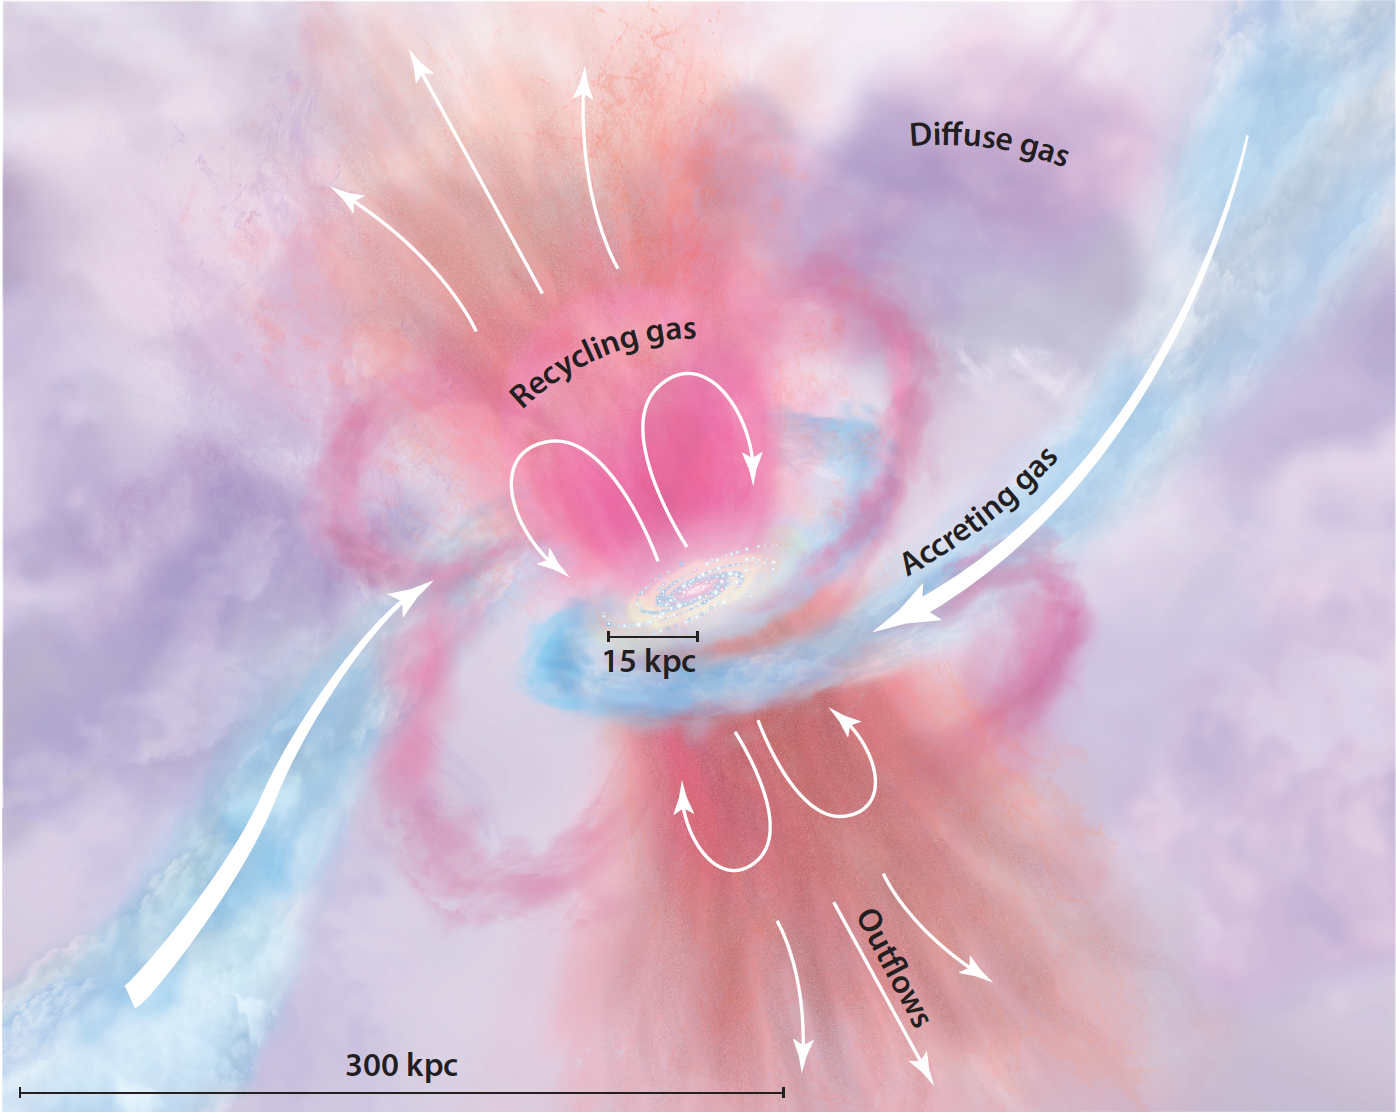
\includegraphics[width=0.8\textwidth]{plots_chp1/CGM_Tumlinson_2017.png}
 \caption[A general view of a galaxy's circumgalactic medium (CGM)]{An idealised illustration of the circumgalactic medium offered by \citet{tumlinson2017}.}
 \label{fig:CGM-Tumlinson2017}
\end{figure}

The processes and features referred to in Fig. \ref{fig:CGM-Tumlinson2017} are: (a) the inflow or accretion of pristine gas from the IGM; (b) outflows of gas that may be driven by either stellar and/or AGN feedback events; (c) infall of metal-rich gas that has been expelled from the galaxy at velocities $\varv < \varv_{esc}$ (below the escape velocity); (d) diffuse extensions of low surface-brightness gas. Provided that the cold molecular gas that fuels star-formation is affected by one of or a combination of these mechanisms, the flow of baryons - gas as well as metals or dust - into and out of the CGM plays a very significant role in the evolutionary path that a galaxy follows.

The concept of a CGM only emerged in the astronomy lexicon rather recently. During this time, both observations and simulations, which have improved over the years with the development of new instruments on telescopes and faster computing, have been invoked to study the CGM in greater detail. Observationally, some of the main methods for studying the CGM are: (a) detecting absorption lines in spectra in the transverse direction on the projected plane of a galaxy; (b) mapping out line-emission; (c) stacking spectra from faint sources; (d) detecting line emission and absorption ``down-the-barrel'' or along the line-of-sight; (e) simulating and modelling CGM processes using hydrodynamical simulations and semi-analytic models. Each of these methods have been succinctly outlined by \citet{tumlinson2017} as the following:

(a) The absorbing gas within the CGM of a galaxy, when viewed against a background quasar, is defined by several parameters. The first of these is column density which is simply the number of absorbing ions or atoms per unit area along a sight-line, Doppler widths given by the $b$ parameter which is defined as $b^2 = 2kT/m + b_{nth}$ in which $k$ is the Boltzmann constant, $T$ the temperature of the gas medium, and $m$ is the gas particle mass and $b_{nth}$ is due to intrinsic broadening of emission lines as a result of gas turbulence. Redshifts of the absorbing gas are obtained by fitting Voigt profiles to continuum-corrected absorption lines in nearby galaxies \citep[e.g.,][]{Lehner2015,Bowen2016}, distant lensed quasars \citep{RauchHaehnelt2011,Rubin2015} and distant radio galaxies \citep{vanojik1996,wilman2003}. 

(b) Additionally, emission line maps of radiation from CGM have been made with the use of deep narrow-band imaging \citep{Prescott2015,Arrigoni-Battaia2016}, integral field unit (IFU) spectrographs such as the Keck Cosmic Web Imager (KWCI) as seen in \citet{Cai2018} as well as on the Very Large Telescope (VLT) with Multi-unit Spectroscopic Explorer (MUSE) which provides a spectrum for every pixel in the instrument's field of view \citep[e.g.,][]{Cantalupo2014}. 

(c) Stacking spectra is gainful for detecting weak or faint absorption through the co-addition of hundreds to thousands of spectra from large surveys. (d) Emission and absorption are detected ``down-the-barrel" or along the line-of-sight using spectroscopy. This method relies on line and continuum emission to be by starlight and possibly also an AGN within a galaxy. The emission serves as a background source without which constraints on the absorbing gas in front of the emission line region would not be possible. This way of detecting CGM gas properties is commonly adopted when observers look for direct evidence of inflowing and outflowing gas by tracing where redshifted and blueshifted emission occurs along the line-of-sight \citep{Steidel2010,Heckman2015}. (e) Simulations of a galaxy CGM's temperature, metallicity, and density have been and continue to be an essential way of grappling the effects of baryon flows over cosmological time-scales as they offer a continuous or evolving view of the associated processes \citep{SomervilleDave2015}.

%phases of the CGM
Another important aspect of the CGM is that it is a multi-phase gas medium within which ionised, molecular and neutral gas complexes can be found. The phases of the CGM have been inferred from hydrodynamic simulations such as those of Fig. \ref{fig:phase-diagram-gas-Torrey2019} from \citet{Torrey2019}, which illustrates the expected baryon phases within the gravitationally bound gas halo at $z=0$ as a function of temperature and density. Hot, diffuse gas with $\log{(T/K)} \gtrsim 7$ is predicted by simulations as well and has also been observed in soft X-ray emission \citep{AndersonBregman2010}. The warm, ionised gas medium generally has temperature within the approximate range of $\log{(T/K)} \simeq 4.5 - 6$ with slightly cooler ionised gas having temperatures of $\log{(T/K)} \simeq 4.$ More information about the ionisation conditions and temperatures of ionised gas can be drawn from photoionisation equilibrium models (PIE) such as the spectral synthesis modelling code \pkg{cloudy} \citep{Ferland2013}. 

\begin{figure}
 \centering
 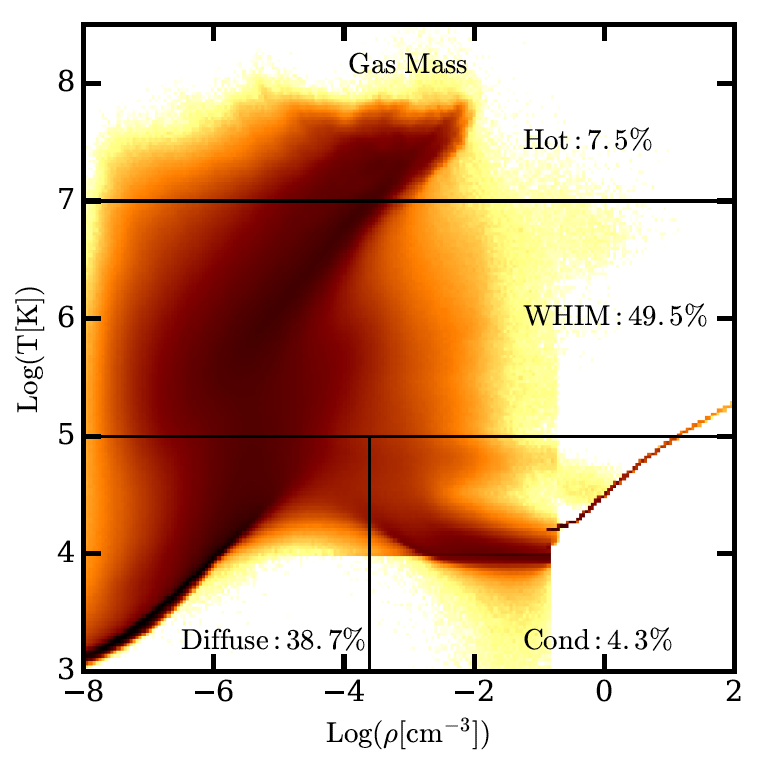
\includegraphics[width=0.7\columnwidth]{plots_chp1/Phase_diag_Torrey2019}
 \caption[Phase diagram of a simulated gas-mass distribution at $z=0$]{Phase diagram of gas-mass distribution at $z=0.$ The boundaries between the different gas phases are given along with the fraction of gas phase to the total gas budget. The gas phases are a hot ($\log{(T/K)} > 7$), warm-hot intergalactic medium (WHIM; $5 < \log{(T/K)} < 7$), diffuse ($\rho < 1000\rho_{\rm c}\Omega_{\rm c}$, $\log{(T/K)} < 5$) and condensed gas ($\rho > 1000\rho_{\rm c}\Omega_{\rm c}$, $\log{(T/K)} < 5$) masses which were coined by \citet{Dave2001} and \citet{Haider2016}. $\Omega_{\rm c}$ and $\rho_{\rm c}$ are critical densities.}
 \label{fig:phase-diagram-gas-Torrey2019}
\end{figure}

One of the major issues facing CGM studies, however, is that of the so-called ``missing baryons''. This has been evinced by CGM masses of low to high luminosity galaxies being lower than the expected cosmological baryon to mass density parameter ratio of $\Omega_{\rm b}/\Omega_{\rm M}=0.16$ determined from observations from the Planck Mission \citep{Planck2016}. Also, measurements of galaxy halo masses have proved that the total measured masses of baryons in galaxies are lower than that which is predicted by  $\Lambda$CDM (cold dark matter) cosmology. In other words, $M_b \ll (\Omega_{\rm b}/\Omega_{\rm M})M_h$ where $M_b$ is the total baryon mass, and $M_h$ the halo mass. An example of this is illustrated in Fig. \ref{fig:CGM-baryon-budget-Tumlinson2017} where the surface gas densities of multiple gas phases and dust when added do not account for the gas surface density predicted by $\Lambda$CDM cosmology. In general, many galaxies appear to be missing up to $80\%$ of their baryons meaning that the majority of baryons in the CGM are currently unaccounted for. It has been suggested that the missing baryons may be contained within the diffuse, hot halo gas medium. The validity of this will be tested in current as well as upcoming X-ray missions such as {\it eRosita} \citep{Merloni2012}, which was launched in July 2019, {\it NuSTAR} (Nuclear Spectroscopic Telescope Array) \citep{Harrison2013} and {\it ATHENA} \citep{Nandra2013}. 

\begin{figure}
 \centering
 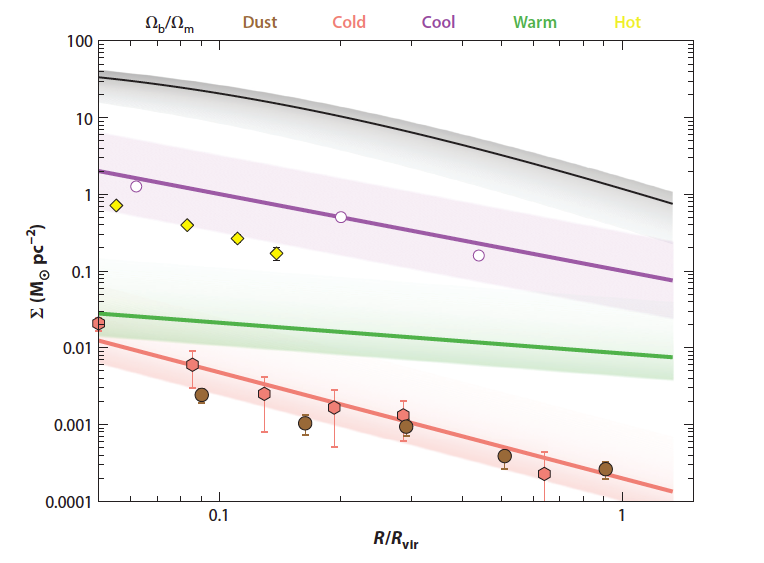
\includegraphics[width=0.8\textwidth]{plots_chp1/CGM_missing_baryons_Tumlinson_2017}
 \caption[Multi-phase CGM mass surface-density profiles]{Synthesis of CGM mass surface-density profiles of multi-phase components compared to the Navarro-Frenk-White (NFW) profile (black) prediction scaled by $\Omega_{\rm b}/\Omega_{\rm M}$ for a dark-matter mass of $M_{\rm DM}/\rm{M}_\odot = 2\times10^{12}.$ The density profiles are for cold gas (salmon) from \citet{ZhuMenard2013a}, cool gas (purple) from \citet{Werk2014}, warm gas (green) traced by \ion{O}{VI} ions \citep{Tumlinson2011,Peeples2014}, hot X-ray emitting gas (yellow) \citep{Anderson2016} and dust (brown) \citep{Menard2010}. }
 \label{fig:CGM-baryon-budget-Tumlinson2017}
\end{figure}

The CGMs of radio galaxies can be studied in great detail because of their bright, extended emission line regions which act as proverbial flash-lights, illuminating the foreground gas within the halo. Observing the CGM also permits one to look for evidence of kinetic feedback beyond just the ISM. 

\subsection{The CGMs of High-redshift Radio Galaxies } 
Observing the kinematics, morphology and ionisation state of gravitationally bound halo gas found around HzRGs is pivotal to understanding how the mechanical power of the radio jets play a role in moderating a galaxy's gas supply. Thankfully, evidence for jet-gas interactions within the gaseous haloes of radio galaxies is plentiful. One of the most effective ways to probe kinematically perturbed gas within the haloes of HzRGs is with emission-line-width measures, particularly the lines that trace the warm, ionised gaseous medium. Most HzRGs are surrounded by giant complexes of ionised gas traced primarily by Ly$\alpha$ emission nebulae \citep{mccarthy1990a,reuland2003}. The Ly$\alpha$ nebulae of HzRGs are known to extend out to to diameters of up to $d \lesssim 200$ kpc. 

%Warm, ionised gas medium
In the rest-frame UV spectral regime spanning $1200 - 1800~\text{\AA}$, the ionised gas medium engulfing a galaxy is probed by rest-UV lines, the most pervasive of which is the Ly$\alpha\lambda$1216. Some of the common lines detected from HzRGs are shown by the composite spectrum of \citet{McCarthy1993} which is a compilation of observed spectral lines in radio galaxy spectra at $0.1 < z < 3$ (see Fig. \ref{fig:comp_spec_RGs}). The emission lines trace the warm, ionised gas regions which have temperatures of approximately, $T_{\rm{e}} \sim 10^{4}-10^{5}$ K, and particle densities of $n_{\rm{e}} \sim 10^{0.5} - 10^{1.5} \rm cm^{-3}$ which are gleaned from emission line diagnostics \citep{OsterbrockFerland2006}. In low density gas regions, forbidden lines which have low transition probabilities are also detected. 
After \citet{reuland2003} used narrow-band imaging to demonstrate that a sample of HzRGs are engulfed by \lya~emitting haloes extending of sizes $d \simeq 100-200$ kpc, it became clear that giant \lya~nebulae are common to many HzRGs. 

\begin{figure}
\centering
  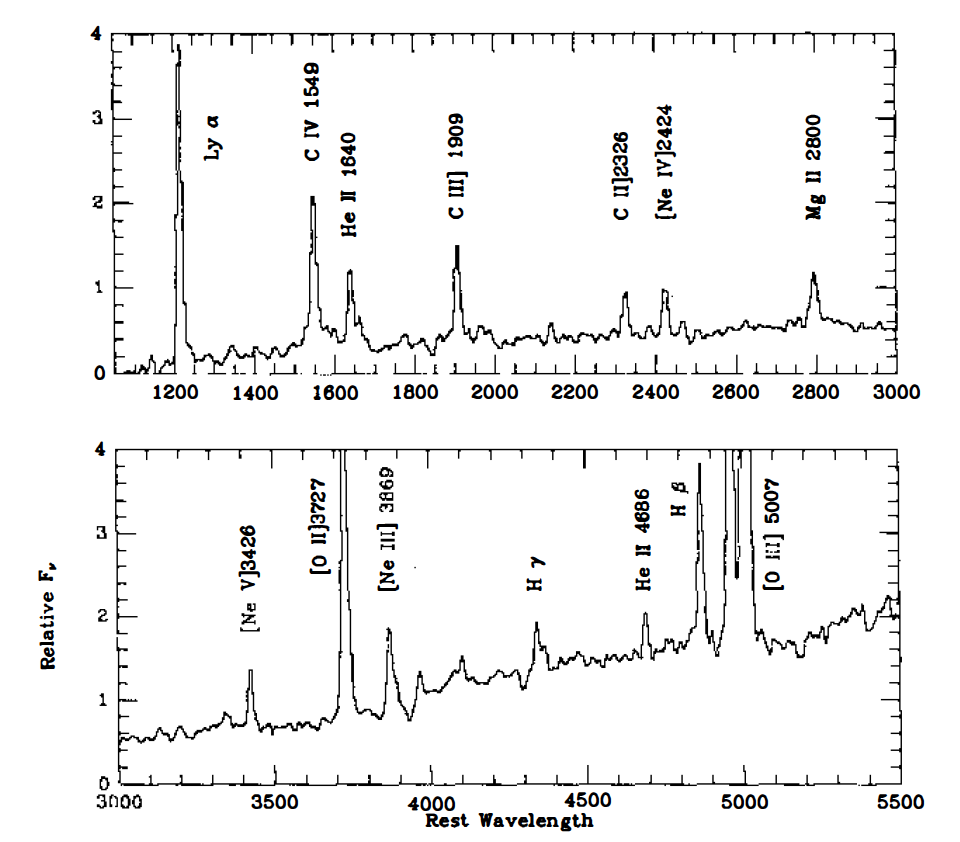
\includegraphics[width=0.65\textwidth]{plots_chp1/UV_spectrum_McCarthy2003}
  \caption[Composite radio galaxy spectrum from galaxies at $0.1 < z < 3$]{Composite radio galaxy spectrum obtained from galaxies at $0.1 < z < 3$ comprising data from the telescopes, Kitt Peak 4 m, Lick 3 m, and Palomar 5 m with $2.5'' \times 3"$ apertures from \citep{McCarthy1993} }
  \label{fig:comp_spec_RGs}
\end{figure}

The high surface-brightness regions within the extended haloes of HzRGs are characterised by turbulent kinematics traced by ionised gas line tracers that are broadened to line-widths of $\rm FWHM \gtrsim 1000$ km s$^{-1}.$ The emission-line gas traced can have luminosities well up to $\rm 10^{44}~erg~s^{-1}$ \citep{mccarthy1996,villar-martin1999a}. In addition to being highly energetic and consisting of turbulent gas motions, the inner halo regions of HzRGs also have clumpy morphologies observed with rest-UV/optical imaging from {\it HST} and spectroscopy from {\it Keck} \citep{humphrey2006,Villar-Martin2006}. The outskirts of HzRG haloes tend to have more quiescent kinematics with line-widths of approximately $\rm FWHM \simeq 100$ km s$^{-1}$ and smoother rest-UV/optical morphologies consistent with gas that is dynamically relaxed \citep{villar-martin2003} (see Fig. \ref{fig:kinematics-ionised-Villar_Martin2003}). 

\begin{figure}[!ht]
 \centering
 \subfloat[]{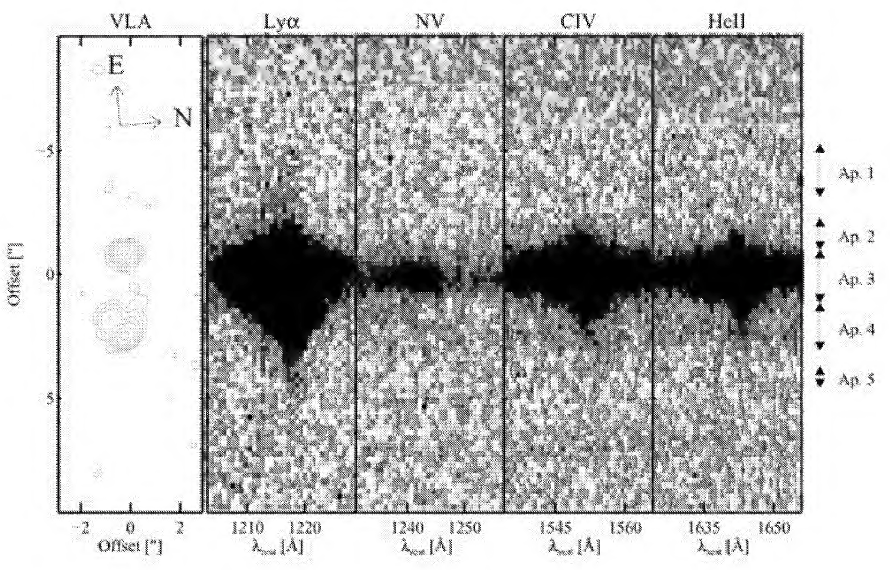
\includegraphics[width=0.7\textwidth]{plots_chp1/pos_velocity_Villar_Martin2003.png}}\\
 \subfloat[]{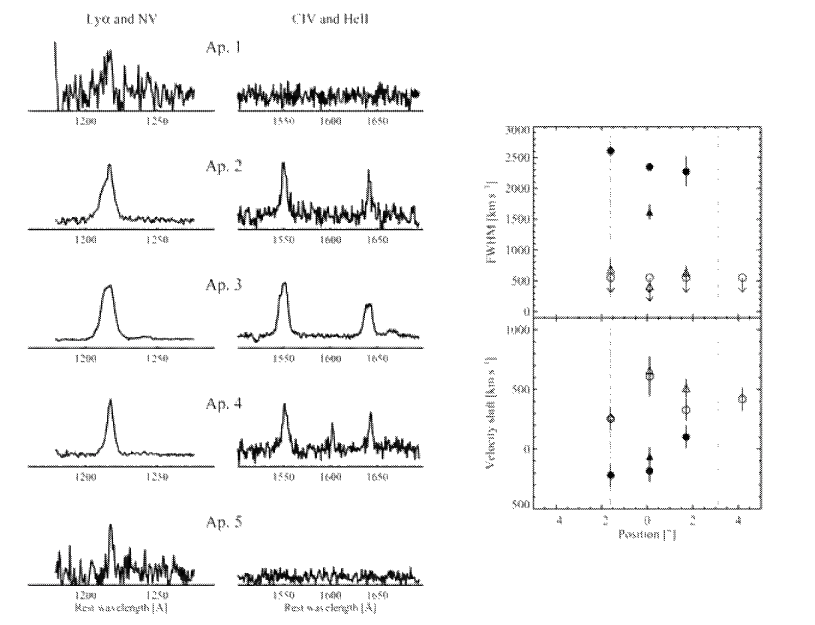
\includegraphics[width=0.7\textwidth]{plots_chp1/spectra_FWHM_vel_shift_Villar_Martin2003.png}}
     \caption[Keck 2D and 1D spectra from \citet{villar-martin2003}]{Panel (a): VLA radio map of the radio galaxy 1809+407 showing Keck 2D spectra (position-velocity diagrams) for Ly$\alpha$ $\lambda$1216, \ion{N}{v} $\lambda$1238, \ion{C}{iv} $\lambda$1550 and \ion{He}{ii} $\lambda1640.$ Panel (b): Spatially integrated spectra from the apertures labelled in panel a (left). The FWHM and velocity offsets relative to \ion{He}{ii} which marks the zero-velocity centroid. The symbols represented are circles for Ly$\alpha,$ and triangles for \ion{He}{ii}; filled symbols for broad components and non-filled symbols for narrow kinematic components of an emission line \citep{villar-martin2003}.} 
 \label{fig:kinematics-ionised-Villar_Martin2003}
\end{figure}

Recent observations of HzRGs using IFU spectroscopy have confirmed much of what has been known of the kinematics and morphology of their gaseous haloes. The IFU spectrograph MUSE, which has a sufficiently good sensitivity to probe extended diffuse emission in the optical, has been important in bringing about a spatially resolved view of emission from ionised gas in the extended gas haloes of distant radio galaxies. In \citet{swinbank2015}, narrow-band imaging of the $z=4.1$ radio galaxy (TN J1338-1942) reveals its colossal $\sim$150 kpc diameter Ly$\alpha$ nebula. Mapping out the velocity in this source showed that it has a velocity gradient of up to $\sim$1000 km s$^{-1}$ along the extent of its nebula (as shown in Fig. \ref{fig:TNJ1338-Swinbank2015}). MUSE IFU data was also important in showing the morphologies of emission in the galaxy MRC 0943-242 from Ly$\alpha$ as well as other rest-UV lines such as \ion{He}{ii} $\lambda1640$, \ion{C}{iv} $\lambda1550$ and \ion{C}{iii]} $\lambda1907$ and \ion{C}{ii]} $\lambda2326$ \citep{Gullberg2016a,Silva2018}. 

\begin{figure}[!ht]
 \centering
 \subfloat[]{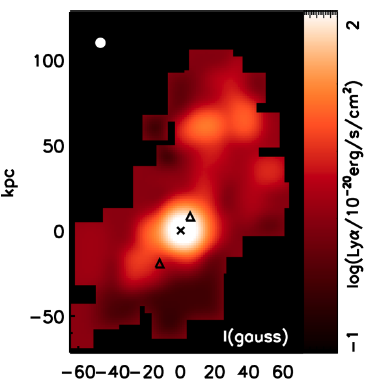
\includegraphics[width=0.5\columnwidth]{plots_chp1/Ly_alpha_intensity_Swinbank2015}}\\
 \subfloat[]{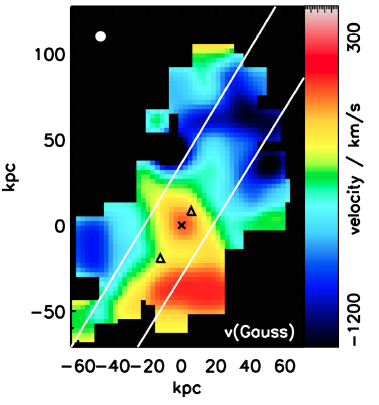
\includegraphics[width=0.5\columnwidth]{plots_chp1/vel_map_Swinbank2015}}
 \caption[Intensity and velocity map from \citet{swinbank2015}]{Panel (a): An intensity map of the underlying Ly$\alpha$ emission profile (modelled by a Gaussian). Panel (b): Velocity map of the Gaussian emission profile from panel (a). The nucleus is shown as a cross and the radio hotspots as triangles. The white lines represent the orientation of the slit along which the velocity shear and \ion{H}{i} column density profiles are seen in spectra extracted from a 9-h observation of the source using the VLT and integral field unit (IFU) spectrograph MUSE (Multi-unit Spectroscopic Explorer) \citep{swinbank2015}.}
 \label{fig:TNJ1338-Swinbank2015}
\end{figure}

The neutral phase of the gas haloes of HzRGs can be probed via Ly$\alpha$ absorption. The absorption troughs superimposed by Ly$\alpha$ emission lines originate from neutral hydrogen located in front of the extended emission line regions along the line-of-sight \citep{rottgering1995,vanojik1997}. The neutral gas which when fit with Voigt profiles is found to have neutral hydrogen (\ion{H}{i}) column densities of $ N_{\rm \ion{H}{i}} /\rm{cm}^{-2} \simeq 10^{18}-10^{20}$ may be associated with the galaxy (located within its ISM or CGM) or be a part of intervening absorption and therefore part of the Ly$\alpha$ forest with $N_{\rm \ion{H}{i}} /\rm{cm}^{-2} \simeq 10^{13} - 10^{15}$ \citep{wilman2004}. In addition to Ly$\alpha,$ other resonant lines such as \ion{C}{iv} $\lambda1550,$ \ion{N}{v} $\lambda1238$ and \ion{Si}{iv} $\lambda1402.$ The neutral phase can also be probed via direct \ion{H}{i} 21cm absorption which has already been done for the $z=3.4$ galaxy B2 0902+34 \citep{Uson1991}. With higher sensitivity radio interferometers which will come online within the next two decades, this direct detection of \ion{H}{i} will become possible for fainter sources. 

The molecular phase of HzRG haloes can be traced via the various fine-structure transitions of the carbon monoxide (CO) molecule. $^{12}$CO emission lines trace molecular hydrogen (H$_2$) due to collisional excitation of CO by the H$_2$ molecule which result in emission from the rotational transitions $J=1\rightarrow0, 2\rightarrow1, 3\rightarrow2, 4\rightarrow3$ and $5\rightarrow4$ \citep{SolomonvandenBout2005}. Several HzRGs have been detected in these CO transitions \citep{Scoville1997,Alloin2000,deBreuck2003,Papadopoulos2000,
Greve2004,deBreuck2005,Klamer2005,Ivison2008,Emonts2014,emonts2015,Gullberg2016b}. The observations that provided these results were obtained from milimetre/sub-milimetre interferometry on instruments such as Australia Telescope Compact Array (ATCA), Owens Valley Radio Observatory (OVRO), IRAM 30 m telescope, Plateau de Bure Interferometer (PdBI), Atacama Pathfinder Experiment (APEX) and the Atacama Large Millimeter/sub-millimeter Array (ALMA) among others. 

\citet{PapadopoulosGreve2004} were first to demonstrate that emission from the fine-structure transitions in atomic carbon can trace H$_2$ in low-redshift ($z\sim0.018 - 0.043$) ultra-luminous infrared galaxies (ULIRGs). The study showed that the scatter in the [\ion{C}{i}]/CO luminosity ratio is small; in other words, the H$_2$ masses derived from [\ion{C}{i}] and CO lines are consistent. Since then, [\ion{C}{i}]$^3$P$_1 - ^3$P$_0$ and [\ion{C}{i}]$^3$P$_2 - ^3$P$_1$ have been widely used to trace the molecular clouds from which stars form \citep{Alaghband-Zadeh2013,Bothwell2017,Popping2017,Andreani2018,Lelli2018,emonts2018,
Nesvadba2019,Man2019}. A remarkable example of [\ion{C}{i}](1-0) detections that extend far out into the CGM of the Spiderweb Galaxy is presented in \citet{emonts2018} (shown in Fig. \ref{fig:CI-Spiderweb-Emonts2018}). 

\begin{figure}
 \centering
 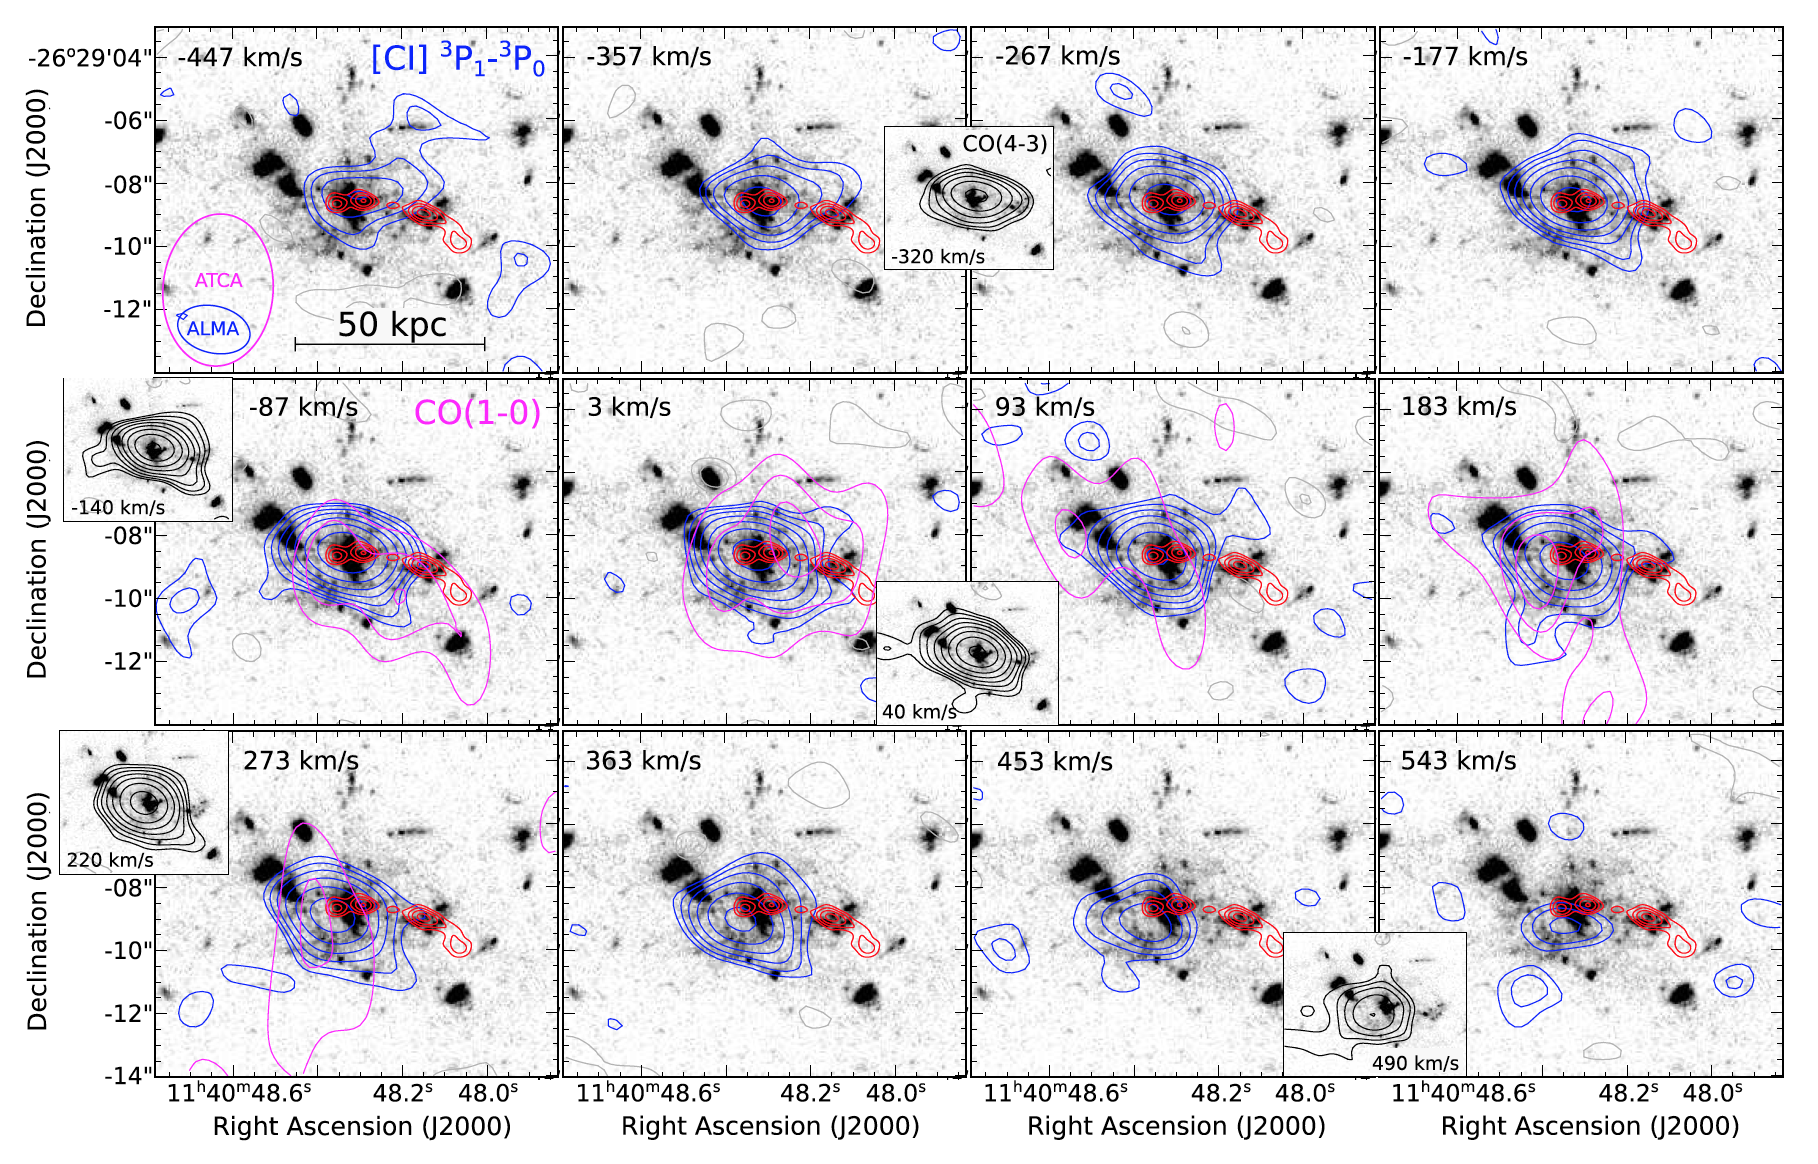
\includegraphics[width=\textwidth]{plots_chp1/Spiderweb_glx_CI_Emonts2018.png}
 \caption[Channels maps of CO(1-0) in MRC1138-262 from \citet{emonts2018}]{Channels maps of the [\ion{C}{i}]$^3$P$_1-^3$P$_0$ emission (blue contours) overplotted over an HST/ACS F475W+F814W image from \citet{Miley2006}. The magenta contours indicate the previously detected CO(1-0) emission and the insets show prominent features detected at other velocity channels. Contour levels of [\ion{C}{i}] and CO(4-3) start at $2\sigma$ and increase by a factor of 1.5, with $\rm \sigma=0.07~mJy~beam^{-1}$ (negative contours are shown in grey). CO(1-0) contour levels are at $2\sigma,$ $3\sigma,$ $4\sigma,$ $5\sigma$ for $\rm \sigma=0.086~mJy~beam^{-1}.$ The red contours indicate the 36 GHz radio continuum from \citet{Emonts2016}.}
 \label{fig:CI-Spiderweb-Emonts2018}
\end{figure}

Overall, observations of distant radio galaxies obtained in the optical, infrared, mm/sub-mm have provided a substantial proportion of evidence suggesting that the gaseous nebulae around HzRGs can be extensive in size $d \gtrsim 200$ kpc. Thermal broadening of line such as Ly$\alpha$ which trace the ionised gas in the halo have suggested that the innermost regions of galaxy haloes up to $d \lesssim 50$ kpc from the AGN more turbulent kinematics than the regions of ionised gas further out \citep{villar-martin2003}. This is quite indicative of how influential radio jets may be in driving ISM gas kinematics. 

Still some questions remain. Do the radio jets alone drive these extreme kinematics? The neutral gas traced by absorption in the resonant line Ly$\alpha$ reveals what may be absorption from the Ly$\alpha$ forest or neutral reservoirs of gas within the CGMs of HzRGs. How does this neutral gas find its way into the CGM - is it accreted along filaments from the IGM or expelled from the host galaxy by AGN feedback? If so how may we observe this? As mentioned earlier, molecular hydrogen is traced by CO and [\ion{C}{i}] lines show that giant molecular clouds also occur up to hundreds of kpc from their host galaxy nuclei within the CGM. Does this H$_2$ gas have primordial origins or is it detected within the CGM as a result being expelled by an AGN feedback event? 

In order to answer questions concerning the kinematics, chemical and morphological structure of the CGMs of distant radio galaxies, deeper observations of such galaxies are required. The CGM maintains the imprints of baryon flows which makes it a kind of forensic tracer for the astrophysical processes that are central to how a galaxy evolves. Coupling these observations with the results of resolved simulations matched in distance scale will provide better insight into the workings of gas within CGM.

% -------------------------------------------------------------------------------------
%           												Section 1.4
% -------------------------------------------------------------------------------------
\section{General Thesis Outline}
% What is the purpose of this thesis?
% What does it aim to achieve ?
% How does it do this?

The main goal of this thesis is to demonstrate that the mechanical power of radio jets play a significant role in altering the morphology, kinematics and ionisation state of the multi-phase gaseous environment from the ISM to the CGM at the $\gtrsim$200 kpc distance scale. We explore this topic in three separate studies. 

\subsection{Chapter 2}
In chapter 2, I have explored the influence of radio-jets on the $<1$Mpc-scale environment density. With the use of a nearest neighbour pseudo-3D density measure, I quantify group scale environments of 2716 radio sources within a 100 deg$^2$ area of the Stripe 82 equatorial field. The radio-jet power is traced using 1.4 GHz luminosities (L$_{1.4~\rm GHz}$) detected from the VLA in the CnB configuration. A statistical correlation test between the galaxy number densities measured to the 2$^{nd}$ and 5$^{th}$ nearest neighbours and radio jet power for radio sources up to $z \sim 0.8$ is carried out. This is achieved by comparing the environment density measures of radio-selected AGN to optical sources that are matched by $K-$band magnitudes and $(g-K)$ colour indices. 

This chapter is based on a published paper of which I am the first author. Thus, I carried out the majority of the work which included scripting the \pkg{python} code required to obtain all of the main results. I was also responsible for assembling the initial and follow-up drafts of the publication which included finding most of the relevant literature required to interpret and discuss our findings. 

\subsection{Chapter 3}
Chapter 3 is a single-source paper. In it, I have used MUSE data to explore the kinematics of ionised and neutral gas within the ISM and CGM of a $z=2.92$ radio galaxy, MRC 0943-242. I did so by parametrising rest-UV lines detected around the nucleus in terms of their emission components which I fit using multivariate Gaussian functions. The resonant rest-UV lines permit us to quantify absorption and I fit these with composite Voigt and Gaussian functions. I compared the column densities obtained from Voigt profile fitting to predictions based on photoionisation models with \pkg{cloudy}. The dominant ionising mechanism powering the metal-rich absorbers is also determined in addition to the distances of the absorbers from the ionising source. 

For this published paper, I reduced the data via the standard ESO reduction pipeline, \pkg{esorex}, for IFU data which produced the final datacube which was analysed to obtain the results reported via \pkg{python} scripts that I wrote. As the first author, I drafted and completed the final draft for submission to the journal. 

\subsection{Chapter 4}
In chapter 4, I have taken ALMA [\ion{C}{i}]$^3$P$_1$ - $^3$P$_0$ line and continuum observations within a $40 \times 40$ arcec$^2$ field of view for seven radio galaxies between $2.9 \lesssim z \lesssim 4.6.$ The [\ion{C}{i}](1-0) line traces molecular hydrogen, which I have used to constrain the masses and kinematics of H$_2$ masses in the ISM and CGM gas regions of the HzRGs. 

For this chapter, I reduced and imaged the interferometric observations using the  reduction pipeline, \pkg{casa} (Common Astronomy Software Applications). I developed the \pkg{python} code required to obtain the results shown in the form of images and spectra and assembled the literature needed for the interpretation and discussion. 
  \chapter[The Influence of galaxy density on radio AGN power]{The relation between galaxy density and radio jet power for 1.4 GHz VLA selected AGN in Stripe 82}

{\it Published in Monthly Notices of the Royal Astronomical Society, Volume 482, Issue 4, p. 5156-5166\\
Authors: {\bf S. Kolwa},
M.J. Jarvis,
K. McAlpine, and
I. Heywood} \\

\section*{Abstract}
Using a Karl G. Jansky Very Large Array (VLA) L-band (1-2 GHz) survey covering $\sim100$\,deg$^2$ of the Stripe 82 field, we have obtained a catalogue of 2716 radio AGN. For these sources, we investigate the impact of galaxy density on 1.4 GHz radio luminosity ($L_{1.4}$). We determine the close environment densities of these sources using the surface density parameter, $\Sigma_N,$ for $N=2$ and $N=5,$ which we bin by redshift to obtain a pseudo-3D galaxy density measure. Matching the radio AGN to sources without radio detections in terms of redshift, $K-$band magnitude and ($g-K$)-colour index, we obtain samples of control galaxies and determine whether radio AGN environments differ from this general population. Our results indicate that the environmental density of radio AGN and their radio luminosity are not correlated up to $z \sim 0.8$, over the luminosity range $10^{23} < (L_{1.4} / $W~Hz$^{-1}) < 10^{26}$. We also find that, when using a control sampled matched in terms of redshift, $K-$band magnitude and colour, environments of radio AGN are similar to those of the control sample but with an excess of overdense regions in which radio AGN are more prevalent. Our results suggest that the $<1$ Mpc-scale galaxy environment plays some role in determining whether a galaxy produces a radio AGN. The jet power, however, does not correlate with environment. From this, we infer that secular processes e.g. accretion flows of cold gas to the central black-hole are more critical in fuelling radio AGN activity than radio jet power is.
 
\section{Introduction}

Through recent developments in the study of galaxy evolution, it has become clear that active galactic nuclei (AGN) activity may play a critical role in the evolution of galaxies (see \citealt{heckman2014} and references therein). Semi-analytic models and hydrodynamic simulations have both introduced a requirement for physical mechanisms that terminate and/or regulate star formation in the most massive galaxies in order to reproduce the galaxy luminosity function \citep[e.g.][]{im2002,wolf2003,mauch2007,siana2008,yuan2016}. 

Many of these models have also proved that galaxies also require physical processes that would explain the relation between the black-hole mass and stellar bulge mass or host galaxy stellar mass \citep[$M_{\rm{BH}}$-$M_{\rm bulge}$ or $M_{\rm{BH}}$-$M_*$ relation; e.g.][]{miyoshi1995,kormendy2013} or stellar velocity dispersion \citep[$M_{\rm{BH}}$-$\sigma$ relation; e.g.][]{ferrarese2000,gebhardt2000}. A popular proposition to explain both star-formation (SF) regulation and the $M_*$-$\sigma$ relation is feedback. Energy provided by the active supermassive black-hole (SMBH) of a galaxy can both heat and/or expel cold gas from the galaxy halo to quench SF in negative feedback \citep[e.g.][]{springel2005,dimatteo2005,croton2006,bower2006,hopkins2006,ciotti2010} or boost star-formation rate (SFR) in positive feedback \citep[e.g][]{ishibashi2012,zinn2013,silk2013}. Feedback from the central nucleus of the galaxy may also effect the larger scale proto-cluster or cluster environment \citep{RawlingsJarvis2004}. 

Nevertheless, the details of such feedback mechanisms is still open to question, and different mechanisms have been proposed depending on how efficiently the AGN accretes gas, leading to dichotomies that describe feedback based on the accretion efficiency as measured by the bolometric luminosity of the black-hole (BH) ($L_{\rm{bol}}$) relative to its Eddington luminosity ($L_{\rm{Edd}}$). More efficient or ``cold accretion" sources, with $L_{\rm{bol}}$/L$_{\rm{Edd}} \gtrsim$ 0.01, undergo radiative or quasar mode feedback where SF is regulated through outflows \citep[e.g.][]{fischer2010,greene2011,sturm2011,veilleux2013,spoon2013,liu2013,cicone2014}. 

AGN that accrete gas less efficiently in ``hot accretion'' mode ($L_{\rm{bol}}$/$L_{\rm{Edd}}$ $\lesssim$ 0.01) via an advection dominated accretion flow \cite[ADAF;][]{heckman2014}, provide feedback mechanisms that are assumed to originate from their radio emission. The radio jets mechanically work to heat up and inflate halo gas in radio or kinetic mode feedback, where the accretion is from a hot gas reservoir in the halo of a galaxy \citep[e.g.][]{fabian2003,fabian2006,best2006}. 

Given that these two accretion mechanisms rely on the supply of cold gas, either directly from the cool gas in the intergalactic medium, or via pockets within the hot haloes surrounding individual galaxies, the environments of radio AGN should reflect this. Indeed, there have been a multitude of studies investigating the role of environment in relation to AGN activity, however, many of these give conflicting results due to the difficulty in comparing studies based on different depths, wavelengths, environment measures and redshift \citep[e.g.][]{best2004,cooper2005,sorrentino2006,tasse2011,sabater2013,
karouzos2014a,malavasi2015}.

There has, however, been a shift forward in thinking about the link between AGN and environment. This has been brought about by considering how the prevalence of AGN activity not only depends on environment but also how it depends on a galaxy's stellar and/or halo mass \citep[e.g.][]{WilliamsRottgering2015}. In addition to this, how AGN activity depends on the ongoing star formation rate (SFR) within a host galaxy, or simply the SFR within the central regions of a galaxy \citep[e.g.][]{sabater2015}. 

Using deep data across a range of wavebands, \cite{karouzos2014a} investigated how the prevalence of AGN activity depended on the local galactic environment, and found that the main driving force at high redshift may just be that the AGN preferentially reside in the most massive galaxies, rather than any link to galaxy mergers. At lower redshift, a range of studies using the Sloan Digital Sky Survey (SDSS) have started to converge. \citet{sabater2015} found that optical AGN activity at relatively low redshift is predominantly dependent on the overall gas supply into the central nucleus, and secular processes can drive the bulk of AGN activity, whereas the larger scale environment plays a secondary role by influencing this gas supply.

In a study similar to the one undertaken in this paper, \citet{ellison2015} used the SDSS and the NRAO VLA Sky Survey \citep[NVSS;][]{condon1998} to investigate the link between environment at the low-accretion regime where activity is traced by relatively low-power radio galaxies i.e. with $L_{1.4}$ in the range, 10$^{23-25}$~W Hz$^{-1}.$ The findings suggested that while such radio AGN generally reside in more evolved and massive galaxies, the primary route for fuelling the AGN comes via accretion from the surrounding medium or through minor mergers, in addition to an internal mechanism, which they attribute to stellar winds from evolved stars.

% %nature vs nurture
 Also, quite often, by examining AGN environments, more focus is placed on the physical processes occurring well outside the virial radius of the AGN's host galaxy. It is probable however that internal processes e.g. accretion, outflows, AGN feedback, magnetic field variation etc. are just as likely to play a role in triggering, sustaining or shutting off AGN activity \citep{maia2004,best2004,draper2012}. AGN studies that take into account both intrinsic galaxy properties as well as the environment provide a more complete picture. 

The radio emission measures their non-thermal component emission i.e. synchrotron radiation from AGN or star-formation activity \citep{antonucci1993}. In terms of environment, 1.4\,GHz selected AGN ($z < 2$) with radio luminosities, $10^{21-27}$\,W~Hz$^{-1},$ are predominantly found in rich, dense cluster regions when compared to galaxies with weak or undetected radio emission \citep{malavasi2015}. Comparing optical to radio AGN ($0.03 < z < 0.1$), \citet{sabater2013} find that fractions of optical AGN decrease with density while the opposite occurs for radio AGN. Radio-loud (RL) AGN environments are also strongly clustered up to distance scales $\lesssim 1$ Mpc. This suggests that the gas medium at the scale of the dark matter (DM) halo determines both total radio jet power and the probability of a galaxy being a RL AGN \citep{donoso2010,magliocchetti2017,hale2018}.

In this paper we build on these studies and investigate the environmental density around radio AGN by combining a new deep radio survey over the SDSS Stripe 82 field with the existing deep optical data from the SDSS and near-infrared data from the UK Infrared Deep Sky Survey \citep[UKIDSS;][]{lawrence2007}. 

In this paper, we study the close environments of radio selected AGN. The paper is structured in the following way: in Section \ref{section-2}, we summarise the details of the multiwavelength dataset. We also explain the selection method for the radio AGN and three different control samples. In Section \ref{section-3}, we outline the method used to  measure environment. We detail the main results of the study in Section \ref{section-4} and discuss their implications and significance in the context of previous findings on AGN environments. Section \ref{section-5} provides a brief summary of our study and its main conclusions. Throughout this work, we have assumed $\Lambda$CDM cosmology bringing into use the fit parameters from WMAP Nine-year data (WMAP9): H$_{0} = 69.7$ km $\rm{s}^{-1} \rm{Mpc}^{-1}$, $\Omega_{\rm{m}} = 0.237,$  $\Omega_{\rm{k}} = 0.0462$ and $\Omega_{\Lambda} = 0.716$ \citep{hinshaw2013}.

%-------------
% section 2
%-------------
\section{Data and Sample Selection}\label{section-2}

\subsection{VLA 1.4 GHz Survey}
Our parent radio source catalogue is taken from a 1--2\,GHz VLA snapshot survey covering $\sim$ 100 deg$^{2}$ over the SDSS Stripe\,82 field. The survey was carried out with the CnB hybrid configuration and reaches an effective rms of $S \sim 88$\,$\mu$Jy beam$^{-1}$, allowing the detection of low surface brightness features of radio sources. Full details of the survey and the source extraction etc. can be found in \citet{heywood2016}. 

The catalogue contains 8946 5$\sigma$ detections of discrete radio sources with measurements of integrated and peak flux density. In it, each source is assigned three identifiers (IDs) to each radio detection: island, Gaussian and source IDs. In the radio survey images, a $>3\sigma$ (where $\sigma$ is the local RMS noise) detection represents contiguous emission that is identified using the island ID. Gaussian IDs are assigned to each Gaussian fit made in the islands. The source identifier PyBDSF \citep{mohan2015} then determines individual sources within each island and each of these is assigned a source ID. In this work, we make use of the source ID to determine individual sources detections. In cases where multiple detections are contiguous, a single source ID is assigned.

\subsection{SDSS DR7}\label{section-sdss}
The SDSS Stripe 82 covers an area of 275 deg$^{2}$. Here we use the SDSS Stripe 82 Co-added Galaxy Photometric Redshift Catalogue \citep{reis2012}, and impose a magnitude cut in the $g-$band of $g < 24.5$ to reduce photometric redshift uncertainties.

\subsection{UKIDSS DR10} 
The UKIRT (United Kingdom Infrared Telescope) Infrared Deep Sky Survey (UKIDSS) has widely been considered the near-IR survey counterpart to SDSS because of its extensive survey fields that overlap with SDSS fields. We use data from the Large Area Survey (LAS) of UKIDSS which coincides spatially with Stripe\,82. UKIDSS survey data is taken in the \textit{Z,Y,J,H} and \textit{K} filters, reaching a 5$\sigma$ $K-$band Vega magnitude limit of $\sim18.2$ \citep{lawrence2007}. 

\subsection{Multi-wavelength Cross-match}
Cross-matching radio sources with optical and near-infrared counterparts is a notoriously difficult task, with many groups working on delivering automated cross-matching and characterisation algorithms \citep[e.g.][]{prescott2018}. In this paper, we adopt the relatively simple approach of a nearest neighbour to the radio centroid as it is defined for radio sources in the VLA catalogue (see \citet{heywood2016} for further details). 

However, to determine the ideal cross-match radius for multiwavelength counterpart identification, we match two catalogues and compare the distributions of their real and random cross-matches \citep{prescott2016}. We accomplish this by cross-matching both catalogues and selecting all parent catalogue (VLA) sources within a $<20$\,arcsec projected distance from their multiwavelength (SDSS or UKIDSS) counterpart. We do the same for a randomly generated catalogue containing the same number of sources as the parent catalogue, within the same field. 

We then determine the lowest point of convergence between both distributions. The angular separation at this point indicates the boundary between projected separations that represent true or significant matches and those that are merely coincidental. The distributions are shown in Fig.~ \ref{fig:jvla-sdss-dist} where we find that the two cross-matched samples converge at an angular separation of $\sim 2.9$\,arcsec. We, therefore, use this as the separation for which we are confident that the vast majority of optical identifications to the radio sources are real. We note that there will be a small fraction of false identifications, but that these should not significantly effect our results which are purely statistical.

Using this radius, we find 4130 cross-identifications in SDSS, out of the total of 8946 VLA radio sources. The detection limit, in redshift, for the VLA/SDSS sample is $z\sim1.2,$ as shown by Fig.~\ref{fig:jvla-sdss-lum}. We then cross-match the SDSS position to the UKIDSS-LAS catalogue to obtain the near-infrared magnitudes for each source using a cross-match radius of 1~arcsec, yielding 2716 sources with a UKIDSS counterpart. 

\begin{figure}
 \begin{center}
  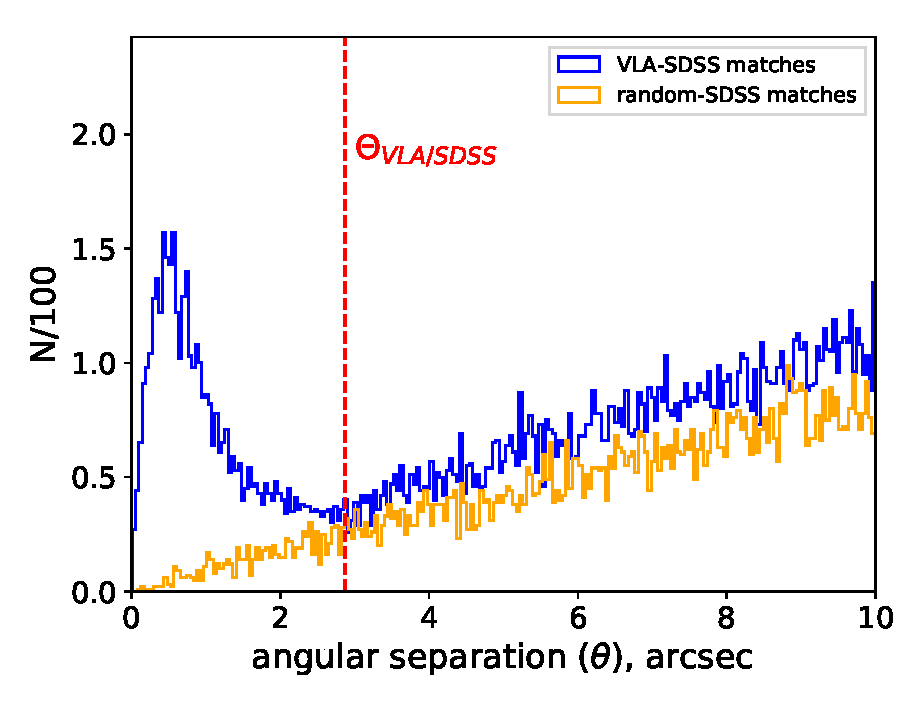
\includegraphics[width=0.75\columnwidth]{plots_chp2/sep_dist_opt.pdf}
  \caption[Cross-match radius determination for VLA/SDSS catalogue]{Distribution of angular separations ($\theta$) between VLA sources and nearest SDSS galaxies (blue) and  between random positions and  SDSS galaxies (orange).}
  \label{fig:jvla-sdss-dist}
 \end{center}
\end{figure}

\begin{figure}
 \begin{center}
   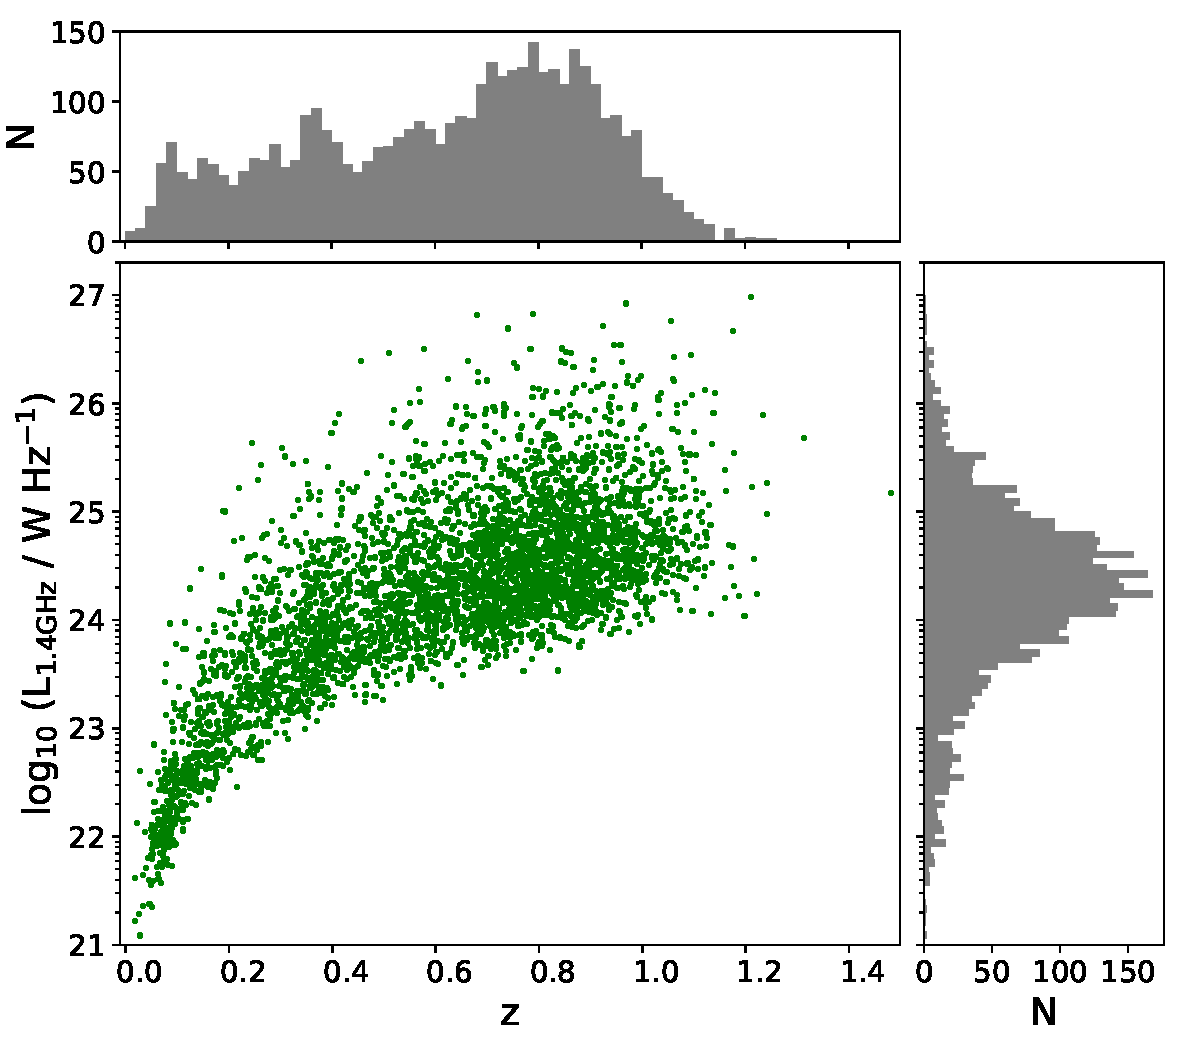
\includegraphics[width=0.8\columnwidth]{plots_chp2/radio_AGN_lum_redshift.pdf}
   \caption[VLA/SDSS source 1.4 GHz radio luminosity redshift diagram]{VLA/SDSS source 1.4 GHz radio luminosity redshift diagram. Redshift and 1.4 GHz luminosity distributions are shown as well. An increasing trend in 1.4 GHz luminosities with redshift represents a Malmquist bias in the radio data.}
   \label{fig:jvla-sdss-lum}
 \end{center}
\end{figure}

\begin{figure}
 \begin{center}
  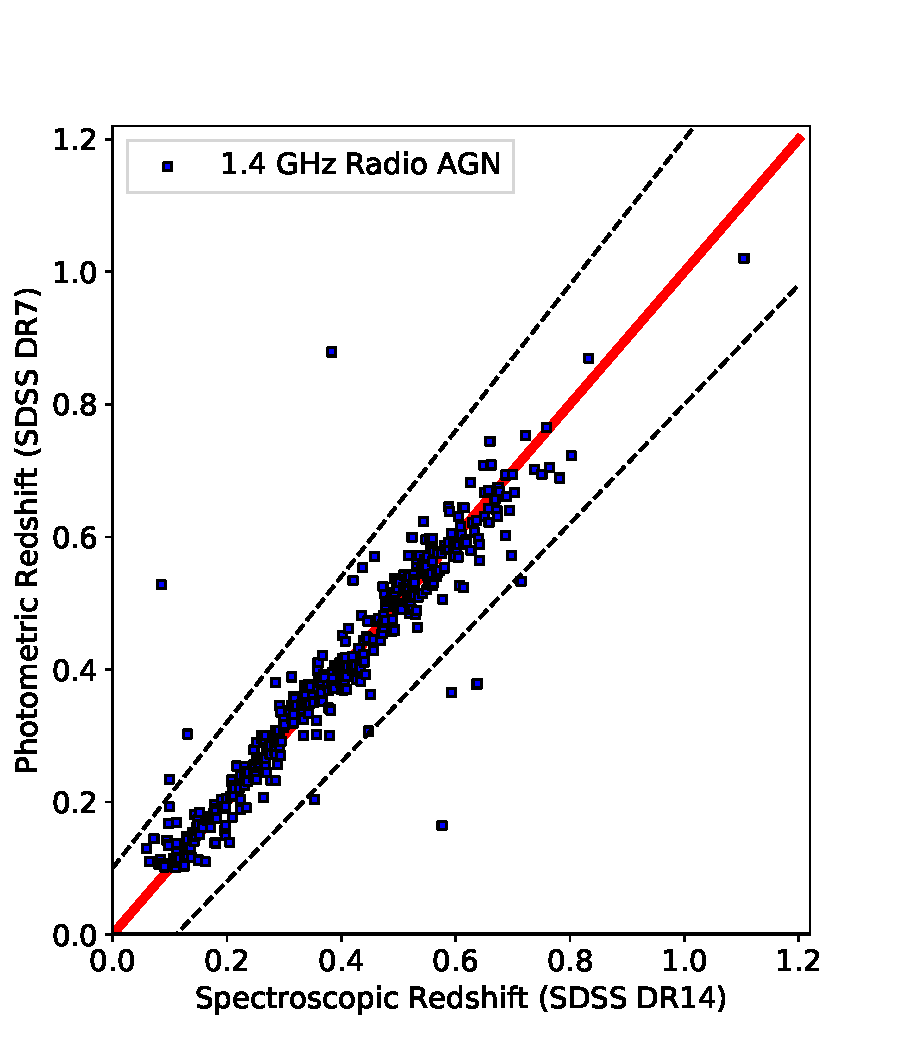
\includegraphics[width=0.8\columnwidth]{plots_chp2/photoz_specz_p.pdf}
  \caption[Comparison of SDSS spectroscopic to photometric redshifts of AGN sample]{Comparison of SDSS spectroscopic to photometric redshifts of AGN sample. The red line represents equality between photometric and spectroscopic redshifts. The dashed lines are the upper and lower limits of the photometric redshift error.}
  \label{fig:photoz-specz}
 \end{center}
\end{figure}

\subsection{Photometric Redshifts}
We choose to only use the photometric redshifts in this study in order to ensure that the comparison of the AGN sample is comparable to that of a control sample, thus by using photometric redshifts we are able to retain the bulk of the cross-identified radio galaxies. However, photometric redshifts ($z_{\rm p}$) are less precise than spectroscopic redshifts ($z_{\rm s}$) and as a consequence reduce accuracy in projected distances and thus surface density measures \citep{cooper2005}. The SDSS DR7 photometric redshift catalogue \citep{reis2012} is complete to $r \sim24.5$ compared to $r \sim17.7$ for the spectroscopic redshifts \citep{york2000}. 

We check the quality of SDSS photometric redshifts by comparing to the spectroscopic redshifts for the radio host galaxies where available. In SDSS DR14, 442 of the VLA radio sources have  spectroscopic redshifts. The photometric redshift estimates against the spectroscopic redshifts are shown in Fig.~\ref{fig:photoz-specz}. We find that 3 per cent i.e. 13 of the 442 sources are discrepant by more than $0.1(1+z_{\rm s}$). Based on this, we conclude that using the photometric redshifts is not likely to bias the density measures for the VLA/SDSS sources.

% --------------
%  section 3
% --------------
\section{Analysis}\label{section-3}

\subsection{Surface Density Estimation}\label{section:env-quant}
There are several methods one can use to quantify the environmental density around galaxies. The chosen method depends on available parameters and the extent to which density is measured. In this work, we use the surface-density parameter, $\Sigma_N,$ 

\begin{equation}\label{eqn:surf-dens}
\Sigma_N = \frac{N}{\pi{d_N}^2}.
\end{equation}

Here, $d_N$ is the projected distance to the $N$th nearest neighbour \citep{dressler1980,gomez2003,mateus2004}. This method requires the exclusion of foreground and background sources via either colour cuts or redshift constraints \citep{kauffman2004,cappellari2011,karouzos2014a,karouzos2014c}. The surface density is advantageous in that it yields a continuous density measure, independent of group or cluster associations \citep{cooper2005}.

To account for separation distances in the radial direction and exclude foreground and background sources, we apply a redshift constraint to Equation~\ref{eqn:surf-dens} which yields a pseudo-3D surface density. Provided that the redshift constraint or velocity interval matches the velocity dispersion of a group or cluster, the local group/cluster density is measured via $\Sigma_N.$ In general, the redshift interval is expressed as $\Delta z = \left| z_i - z_j \right| \leq \varepsilon(1 + z_i)$ for which \textit{i} and \textit{j} are the target and neighbouring galaxies, respectively. $\varepsilon$ is adjusted depending on the radial distance that the density is measured out to and importantly, depends on the accuracy of the redshifts in the sample of interest  

For our analysis, we adopt a conservative value of $\varepsilon =  0.1$, i.e. setting the redshift constraint on AGN surface density $\Delta z  < 0.1(1+z_{\rm{AGN}}),$ where $\Delta z = z_{\rm{AGN}} - z_{\rm{nn}}$ with z$_{\rm{nn}}$ the redshift of the nearest neighbour (nn). Combining this with the surface density measured in projection, we obtain a pseudo-3D AGN density measure, $\Sigma_{N,\rm{AGN}}.$

We are aware that survey artefacts such as point-spread function (PSF)-like features can affect the surface density measure. As explained more fully in Section 3.2 of \citet{heywood2016}, adaptive thresholding in the source finder as well as a manual excision of visually identified artefacts have been used to ensure that the survey contains real source detections. 

Angular masks for bright stars in SDSS can bias surface density measures for either radio AGN or control galaxies that are in close proximity ($\leq150$\,arcsec i.e. the search radius for nearest neighbours) to foreground stars in the survey field. This is not likely to be an issue in the SDSS DR7 galaxy catalogue since the number of bright stars in the Stripe 82 field, i.e. $\sim6\e{5}$ \citep{blanton2005} is significantly lower than the number of SDSS galaxies ($\sim130\e{5}$) from which we select the radio AGN and control samples. Also, given that our final results are drawn from statistical means per $\Delta z = 0.1-0.2$ sized redshift bins, a few bright stars will not affect the mean and median environment measures significantly enough to change the results.

In addition to a redshift constraint, we apply a survey edge correction to refrain from incorrectly measuring the density for sources lying at the edge of the survey field. Measuring surface density for a source located at a projected distance $<d_N$ from the survey edge can result in the $N$th nearest neighbour being located outside the survey field which would lead to an overestimate of $d_N$.  We, therefore, remove radio sources with angular distances $<120$ \,arcsec from the edges of the combined VLA and SDSS/UKIDSS survey fields. In total, 37 radio sources meet this criterion and are removed.

We quantify galaxy environmental density using $N=2$ and $N=5$ in order to measure the close environments of the radio sources at the kpc-scale \citep{karouzos2014a,karouzos2014c}. We subdivide the radio AGN sample into four redshift intervals in order to investigate any evolution in environmental density, whilst also limiting Malmquist bias. The lowest redshift interval spans $0.1 < z < 0.2$ to compare our results to previous low-redshift radio AGN environment studies. The remaining three redshift intervals span $0.2 < z < 0.8.$ 

We note that photometric redshift determination in SDSS is less efficient at z $\geq 0.75$ \citep{reis2012}. This may bias density measures in our sample, as a reasonable portion of the VLA-SDSS sample exist at z $\geq 0.75,$ hence we apply an upper cut to the entire sample at $z\sim0.8.$

\subsection{Radio Source Sample}\label{section:agn-samp}
We determine radio luminosity using flux densities of the $5\sigma$ 1--2\,GHz detections and the photometric redshifts from the SDSS. The sources in our sample lie at $0.1 < z < 0.8$ and we assume a radio spectral index of $\alpha = -0.7$ \citep{condon2002,sadler2002} to $k$-correct to the rest-frame luminosity. 

\subsection{Control Samples}\label{section:control-samp}

In order to assess whether the radio AGN reside in higher density environments compared to the general galaxy population a control sample is required. We construct three separate control samples by matching the radio AGN host galaxies to non-radio AGN galaxies in the SDSS/UKIDSS Galaxy Catalogue in terms of (i) redshift, (ii) redshift and $K-$band magnitudes, and (iii) redshift, $K-$band magnitude and ($g-K$)-colour.

At the relatively low redshifts under investigation here, $K-$band light
is dominated by emission from low mass red stars that form the bulk of the stellar mass, therefore the $K-$band magnitude can be considered a proxy for stellar mass \citep[e.g.][]{gavazzi1996,rocca-volmerange2004}. Similarly, we can take the ($g-K$)-colour index as a proxy for the specific star formation rate (sSFR). These three control samples allow us to identify how the environment of the radio AGN may differ from the field by controlling for key properties of the galaxies. Considering them separately also allows ease of comparison with previous works which may have only accounted for one or two of the parameters considered here.

\begin{table}
\centering
\caption[Sample (iii): 1D and 2D KS-test results]{1D and 2D KS-test results for sample (iii): redshift, $K-$band magnitude and ($g-K$)-colour matched field comparing the distributions for the AGN and control sample.}
\label{table:KScontrol}
\begin{tabular}{l | c c c}
\hline \hline
 Tested samples & Redshift Interval & $D$ & $p$ \\
 & & & \\
  \hline
  Redshift (1D) 					& 0.1 $< z <$ 0.2 		& 0.05 & 0.99 \\
   					 					& 0.2 $< z <$ 0.4 		& 0.04 & 0.92 \\
   										& 0.4 $< z <$ 0.6 		& 0.06 & 0.75 \\
   										& 0.6 $< z <$ 0.8 		& 0.05 & 0.96 \\
                                 
    \hline
   $K-$band magnitude (1D) 				& 0.1 $< z <$ 0.2 		& 0.03 & 0.99 \\
   										& 0.2 $< z <$ 0.4 		& 0.02 & 0.99 \\
   										& 0.4 $< z <$ 0.6 		& 0.03 & 0.99\\
    									& 0.6 $< z <$ 0.8 		& 0.03 & 1.00\\                                   
  \hline
   ($g-K$)-colour (1D) 					& 0.1 $< z <$ 0.2 		& 0.03 & 0.99 \\
   										& 0.2 $< z <$ 0.4 		& 0.03 & 0.99 \\
   										& 0.4 $< z <$ 0.6 		& 0.03 & 0.99 \\
    									& 0.6 $< z <$ 0.8 		& 0.03 & 0.99 \\
  \hline
  Redshift and 							& 0.1 $< z <$ 0.2 	& 0.05 & 0.99 \\
  	$K-$band magnitude (2D) 			& 0.2 $< z <$ 0.4  	& 0.04 & 0.99 \\
                                    	& 0.4 $< z <$ 0.6		& 0.07 & 0.85 \\
                                    	& 0.6 $< z <$ 0.8		& 0.06 & 0.98 \\

  \hline
  Redshift and 							& 0.1 $< z <$ 0.2 & 0.06 & 0.98 \\
  	($g-K$)-colour (2D) 					& 0.2 $< z <$ 0.4 & 0.04 & 0.96 \\
                                    	& 0.4 $< z <$ 0.6 & 0.06 & 0.93 \\
                                    	& 0.6 $< z <$ 0.8 & 0.04 & 0.99 \\
	
  \hline	
  ($g-K$)-colour and 						& 0.1 $< z <$ 0.2 & 0.05 & 0.99 \\
  $K-$band magnitude (2D) 				& 0.2 $< z <$ 0.4 & 0.03 & 0.99 \\
                                    	& 0.4 $< z <$ 0.6 & 0.03 & 0.99 \\
                                    	& 0.6 $< z <$ 0.8 & 0.04 & 0.99 \\
  \hline
  \end{tabular}
\end{table}

We match the radio and control sources according to the following criteria: $\Delta z \leq 0.02(1+z_{\rm{AGN}}),$ $\Delta K \leq 0.05,$ and $\Delta(g-K) \leq 0.1$, where $\Delta$ denotes the difference between the AGN and control sample galaxies in the given observational quantity. The distributions are shown in Figs.~\ref{fig:K-z-control}, \ref{fig:K-z-supercontrol} and \ref{fig:g-K-z-supercontrol}. We perform 1- and 2-D Kolmogorov-Smirnov tests (KS-tests) to check that the distributions in $z$, $K$ and ($g-K$) are indistinguishable between the radio AGN hosts and the control samples. The results of this are shown in Table~\ref{table:KScontrol}. We find that the underlying distributions are indistinguishable for all our sub-samples.

Each radio source in the combined VLA/SDSS/UKIDSS catalogue is matched to a single control galaxy located at an angular separation $>60$\,arcsec from a radio AGN following the criteria in (i), (ii) and (iii). This angular distance constraint is set to reduce the likelihood of the radio source and control galaxy environments overlapping. 

As for the radio AGN, we measure the environmental density around each control galaxy in redshift slices of $| z_{\rm{cont}} - z_{\rm{nn}}| = 0.1(1+z_{\rm{cont}})$, enabling us to compare the radio AGN environments directly with the control sample environments.

\begin{figure}
 \begin{center}
   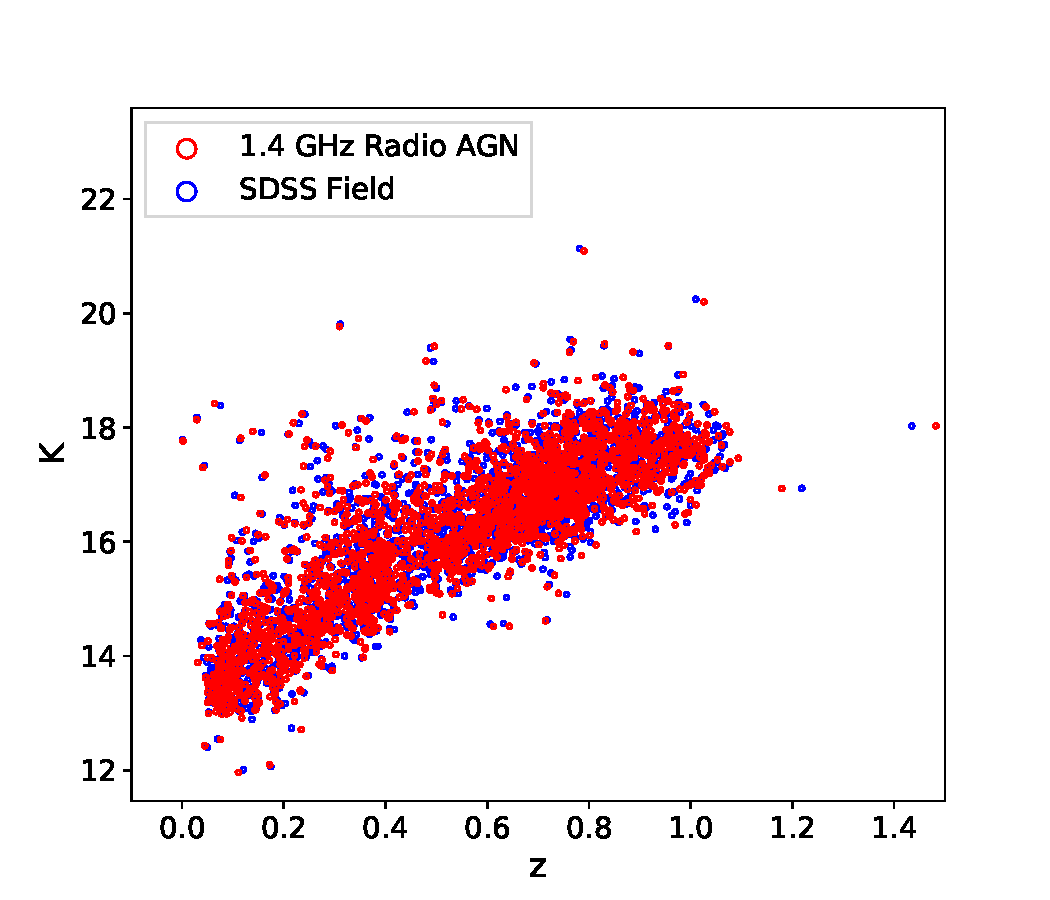
\includegraphics[width=0.8\columnwidth]{plots_chp2/K_z_control.pdf}
   \caption[$K-$band-redshift diagram for radio AGN and sample (ii) control galaxies]{Petrosian $K-$band magnitude as a function of photometric redshift for radio AGN and control galaxies in sample (ii).}
   \label{fig:K-z-control}
 \end{center}
\end{figure}

 \begin{figure}
  \begin{center}
    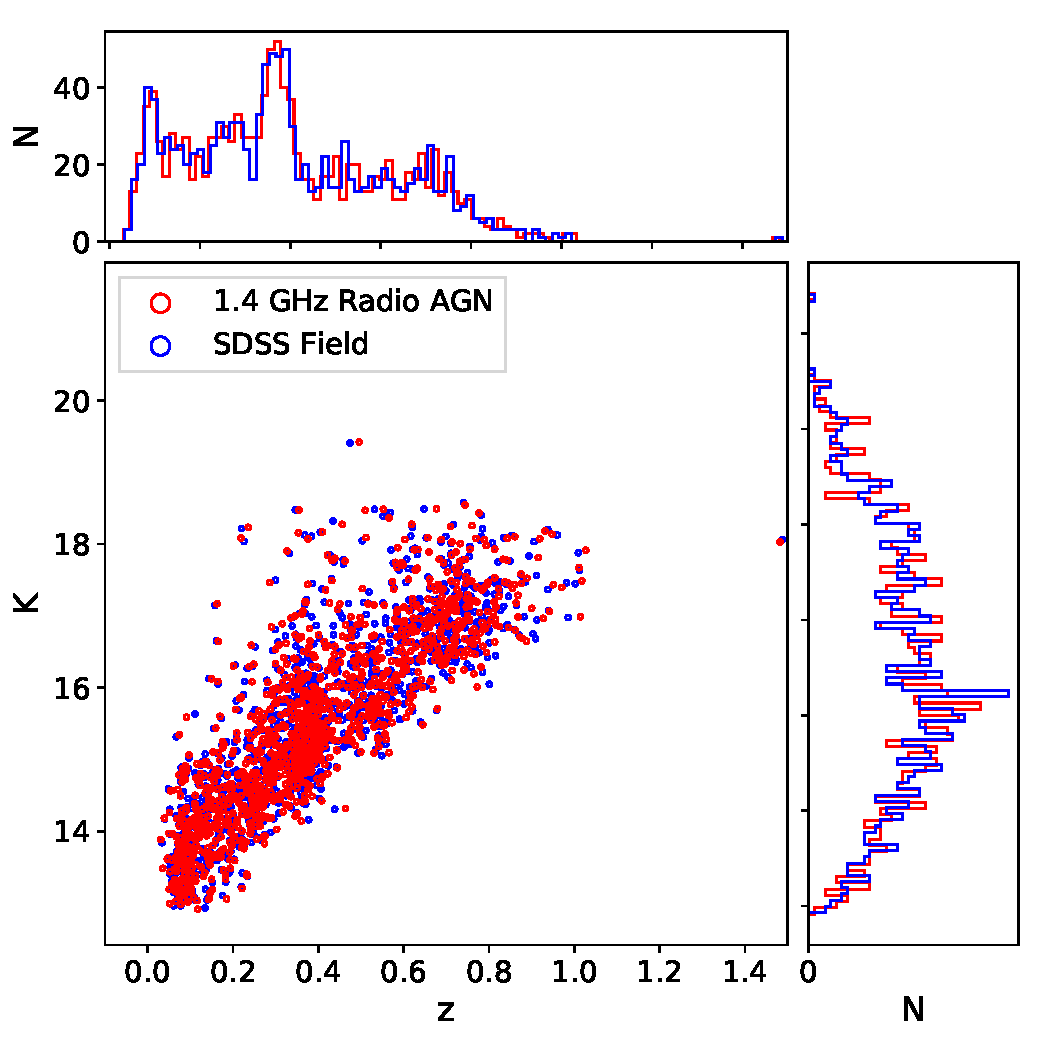
\includegraphics[width=0.8\columnwidth]{plots_chp2/K_z_super_control.pdf}
    \caption[$K-$band-redshift diagram for radio AGN and sample (iii) control galaxies]{Petrosian $K-$band magnitude as a function of photometric redshift for radio AGN and redshift, M$_*$ and sSFR matched SDSS field galaxies in sample (iii). The \textit{1.4 GHz radio AGN} sample is a combination of VLA, SDSS and UKIDSS data. The SDSS field sources (control sample) combined SDSS and UKIDSS.}
    \label{fig:K-z-supercontrol}
  \end{center}
 \end{figure}

\begin{figure}
 \begin{center}
   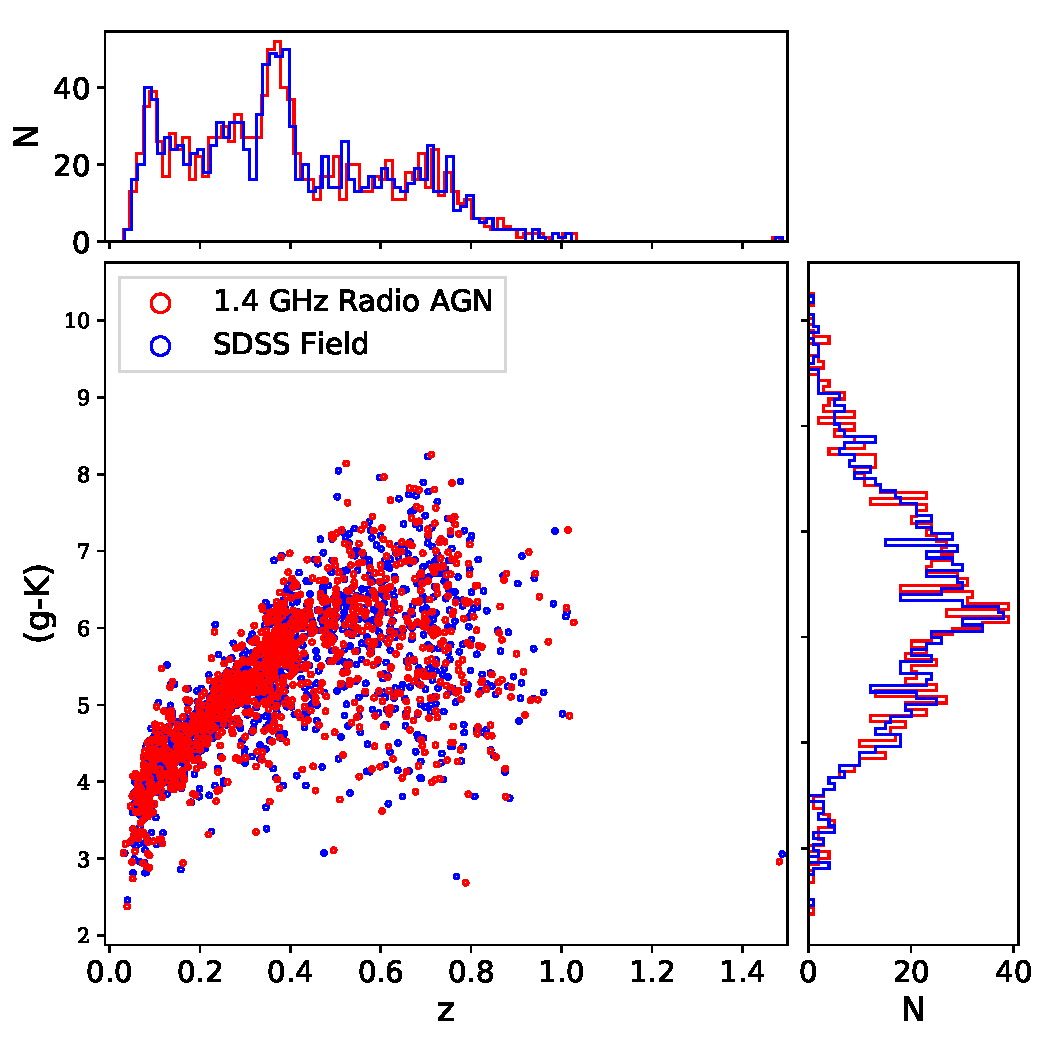
\includegraphics[width=0.8\columnwidth]{plots_chp2/g-K_z_super_control.pdf}
   \caption[($g-K$)-colour-redshift diagram for radio AGN and control galaxies in sample (iii)]{($g-K$)-colour as a function of photometric redshift for radio AGN and control galaxies in sample (iii).}
   \label{fig:g-K-z-supercontrol}
 \end{center}
\end{figure}

\subsection{AGN environment relative to the field} 
The pseudo-3D density of a radio AGN's environment is denoted by $\Sigma_{N,\rm{AGN}}$ and the environmental density for a set of control galaxies matched to a radio AGN is denoted by $\Sigma_{N,\rm{field}}.$

To determine the density of radio AGN environments relative to the field, we take a ratio of these two density measures. Hence, we define $\Sigma_{N,\rm{AGN}}/\Sigma_{N,\rm{field}}$ as the relative density i.e. $\Sigma_{N,\rm{R}}.$ We give this density as both a mean and a median, along with the associated error on the mean, and 16th and 84th percentiles for the median uncertainties. 

Using this, we examine the relation between relative density and $L_{1.4}$ for the radio AGN sample in the 4 redshift intervals spanning 0.1 $< z <$ 0.8. The mean and median relative densities as a function of $L_{1.4}$ for the radio AGN in the redshift slices tell us how jet power correlates with environment density. Spearman's rank correlation parameters $\rho$ and $p$ determine this correlation. For $p < 0.05,$ we reject the null hypothesis that no correlation exists. For environment density as a function of 1.4 GHz radio power the computed correlation test parameters are shown in Table \ref{table:correlation_parameters}. Mean and median density are significant above the $3\sigma$ level in each $L_{1.4}$ bin. Mean and median densities are referred to as $\langle \Sigma_{N} \rangle$ and $\widetilde{\Sigma_{N}}$, respectively. We use two-sample 1D and 2D KS tests to measure the similarity of AGN and control sample environment density distributions. 

\begin{table}
\begin{center}
 \caption[Spearman's rank correlation test for sample (i)]{Spearman's rank correlation test parameters for the relative surface density-$L_{1.4}$ relation for the redshift intervals considered i.e. control sample (i)}
 \label{table:correlation_parameters}
  \begin{tabular}{ c | c c c }
  \hline \hline
 & Redshift Interval & $\rho$ & $p$ \\
 & & & \\
\hline 
  $\frac{\Sigma_{2,{\rm AGN}}}{\Sigma_{2,{\rm field}}}$ 	& 0.1 $< z <$ 0.2 & 0.03 & 0.74	\\
   						& 0.2 $< z <$ 0.4 & 0.00 & 0.99	\\
   						& 0.4 $< z <$ 0.6 & 0.01 & 0.91	\\
   						& 0.6 $< z <$ 0.8 & 0.01 & 0.86	\\         
  \hline                                                                                            
  $\frac{\Sigma_{5,{\rm AGN}}}{\Sigma_{5,{\rm field}}}$ 	& 0.1 $< z <$ 0.2  & 0.16 & 0.04 \\
   						& 0.2 $< z <$ 0.4  & 0.06	& 0.20 \\     
  	 					& 0.4 $< z <$ 0.6  & 0.01 & 0.88  \\         
  						& 0.6 $< z <$ 0.8  & 0.00 & 0.98 	\\
  \hline
  \end{tabular}
 
 \end{center}
\end{table}

\subsubsection{Redshift-matched Control Sample}

\begin{figure*}
\hspace*{-50pt}
  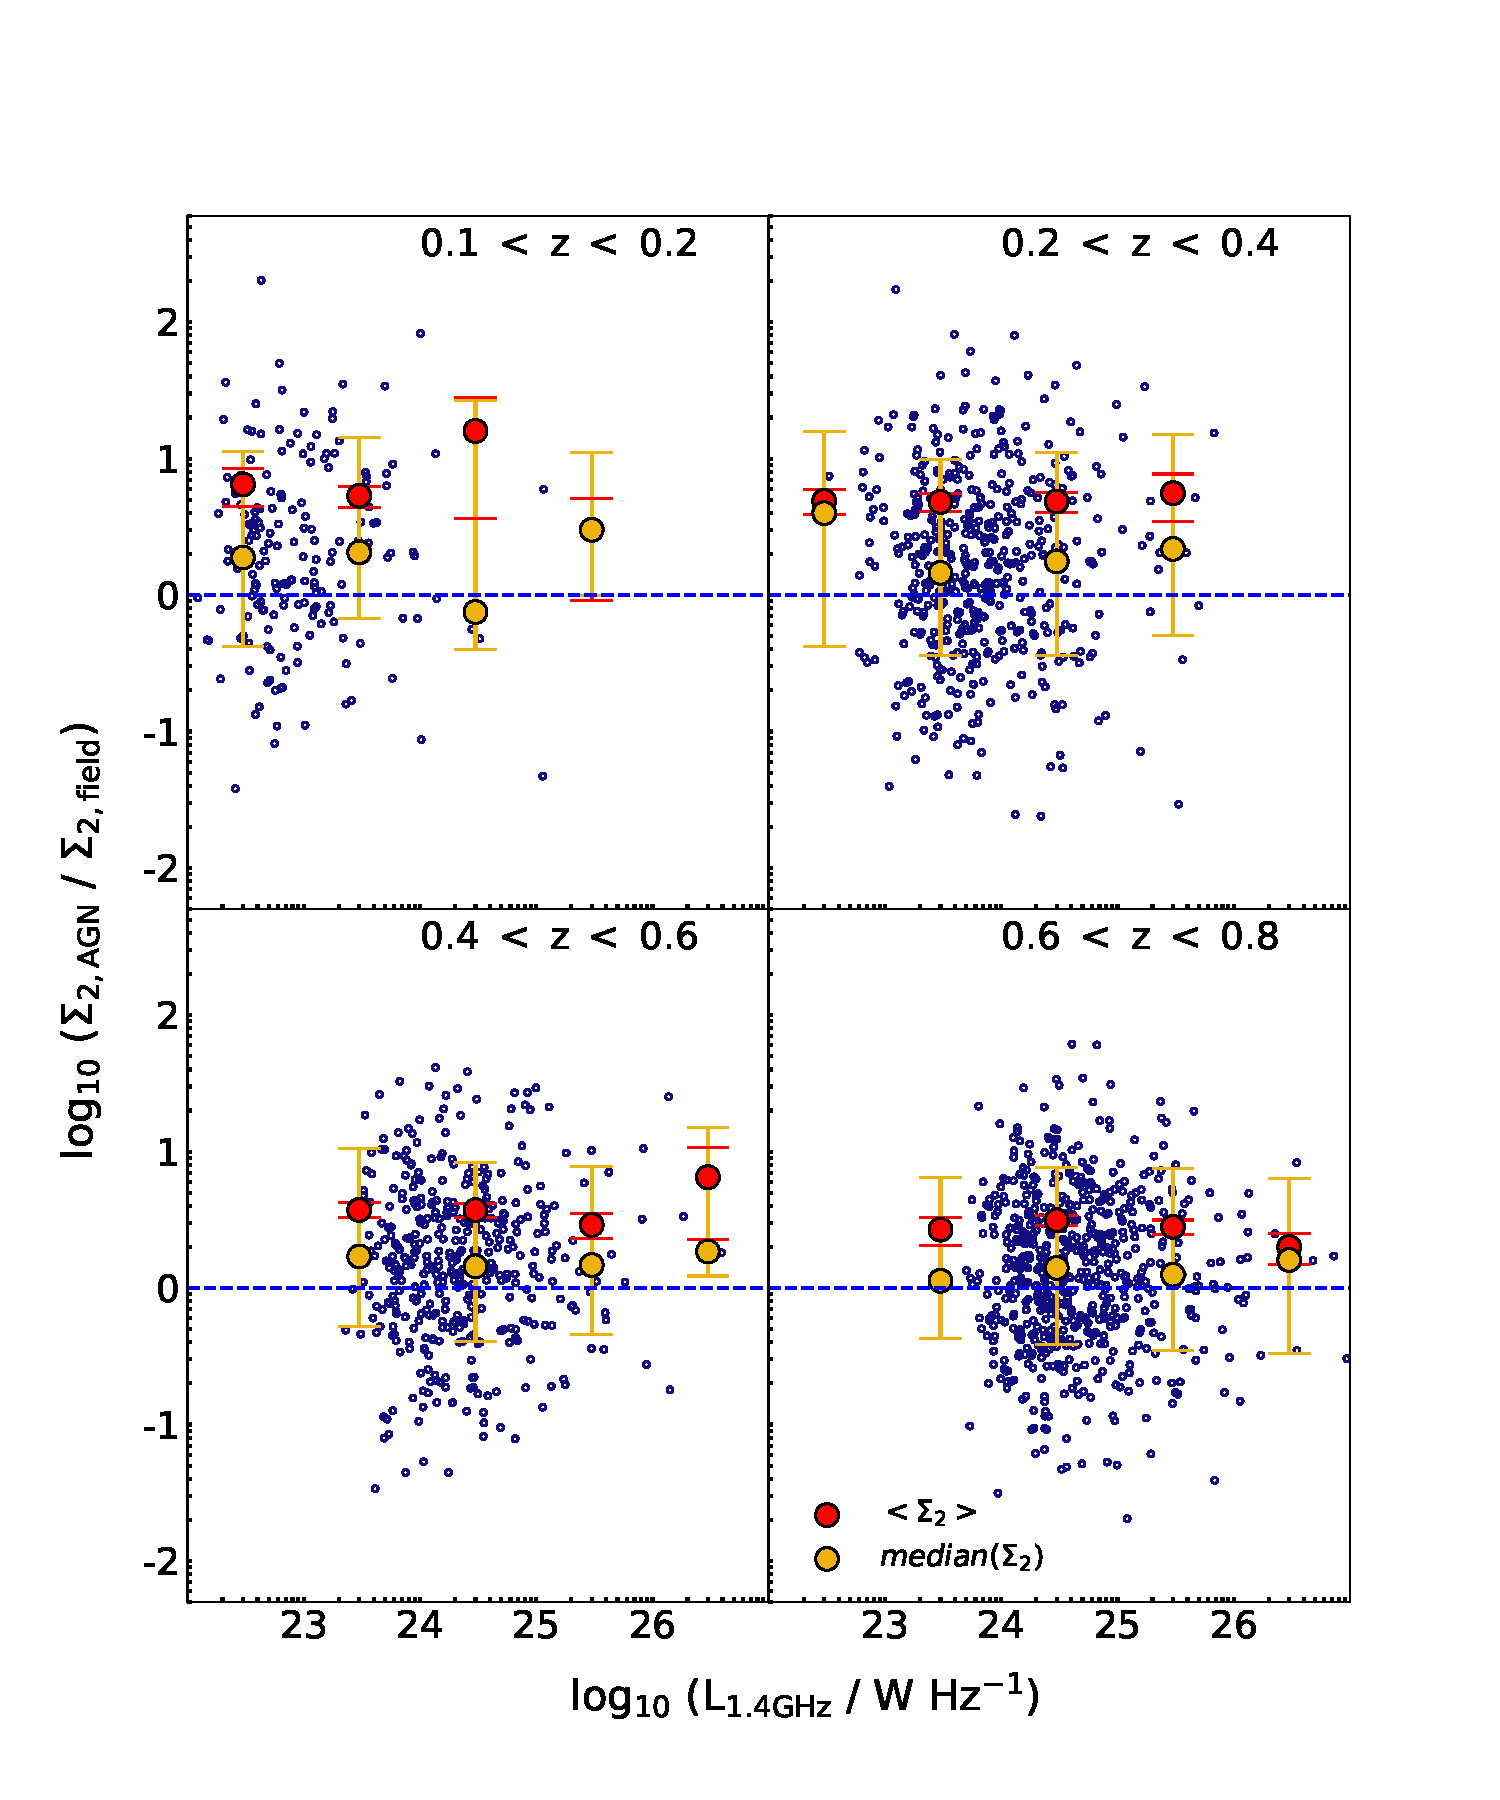
\includegraphics[width=0.6\columnwidth]{plots_chp2/env_L_radio_binned_errs_2_random_control.pdf}
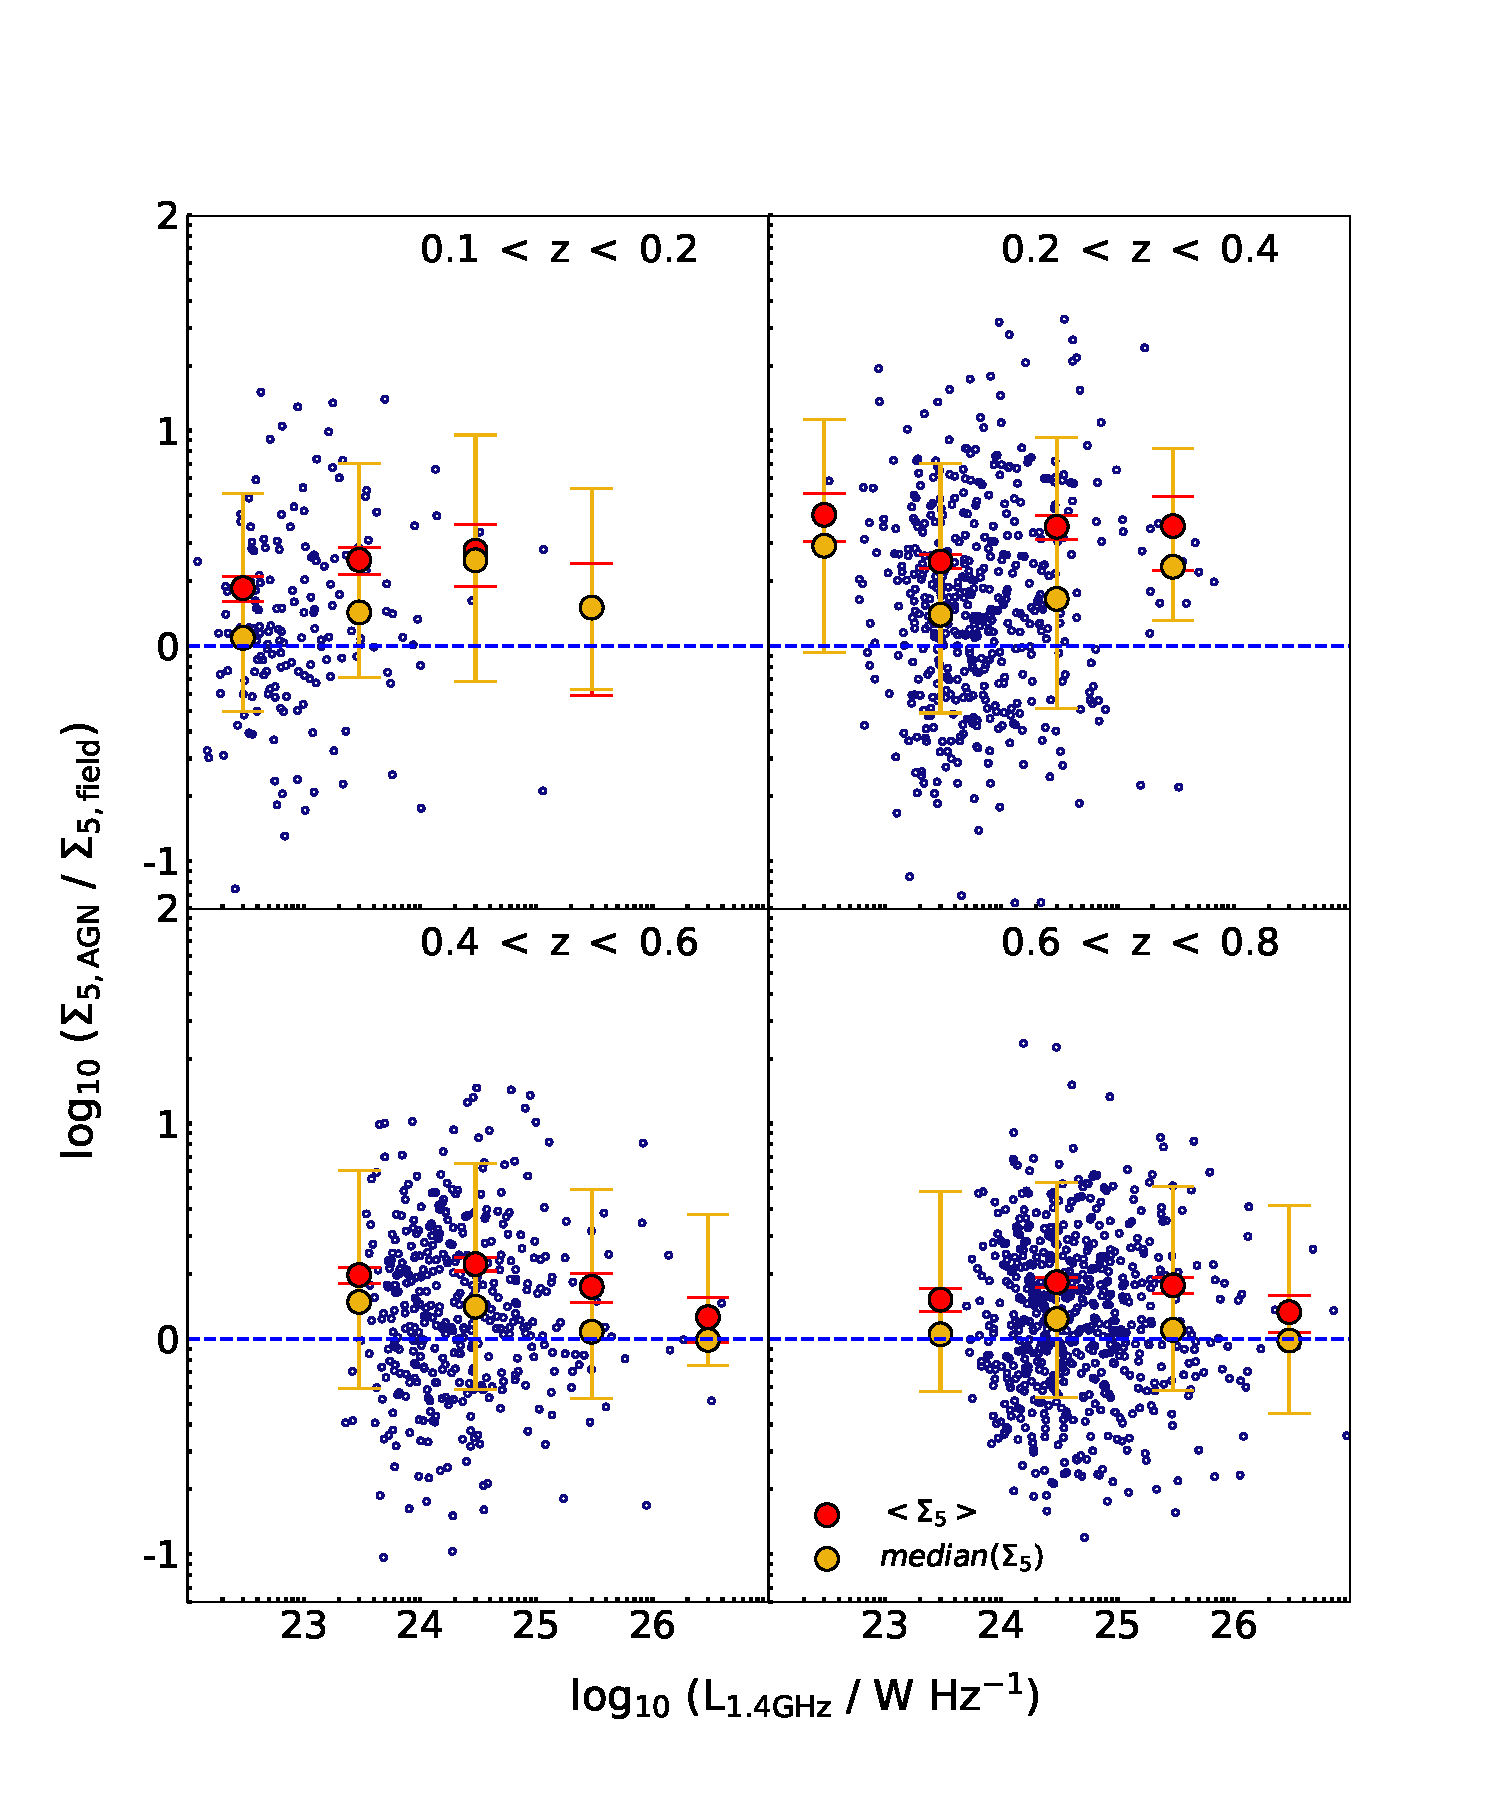
\includegraphics[width=0.6\columnwidth]{plots_chp2/env_L_radio_binned_errs_5_random_control.pdf}
  \caption[Sample (i): Mean and median surface densities, $\Sigma_{2,\rm{R}}$ and $\Sigma_{5,\rm{R}},$ in $L_{1.4}$ bins.]{Mean and median $\Sigma_{2,\rm{R}}$ ($left$) and $\Sigma_{5,\rm{R}}$ ($right$) for the AGN relative to field densities as a function of $L_{1.4}$ for the redshift-matched control sample in 4 redshift intervals. Relative density is denoted by the ratio between AGN and field densities. Mean density ($\langle \Sigma_{2,\rm{R}} \rangle,$ red) and median ($\Sigma_{2,\rm{R}}$, yellow) per $L_{1.4}$ interval are shown. The dashed line denotes the line of equality for the AGN and control sample environments.}
  \label{fig:random-env_L-radio}
\end{figure*}

\begin{figure*}
\hspace*{-50pt}
   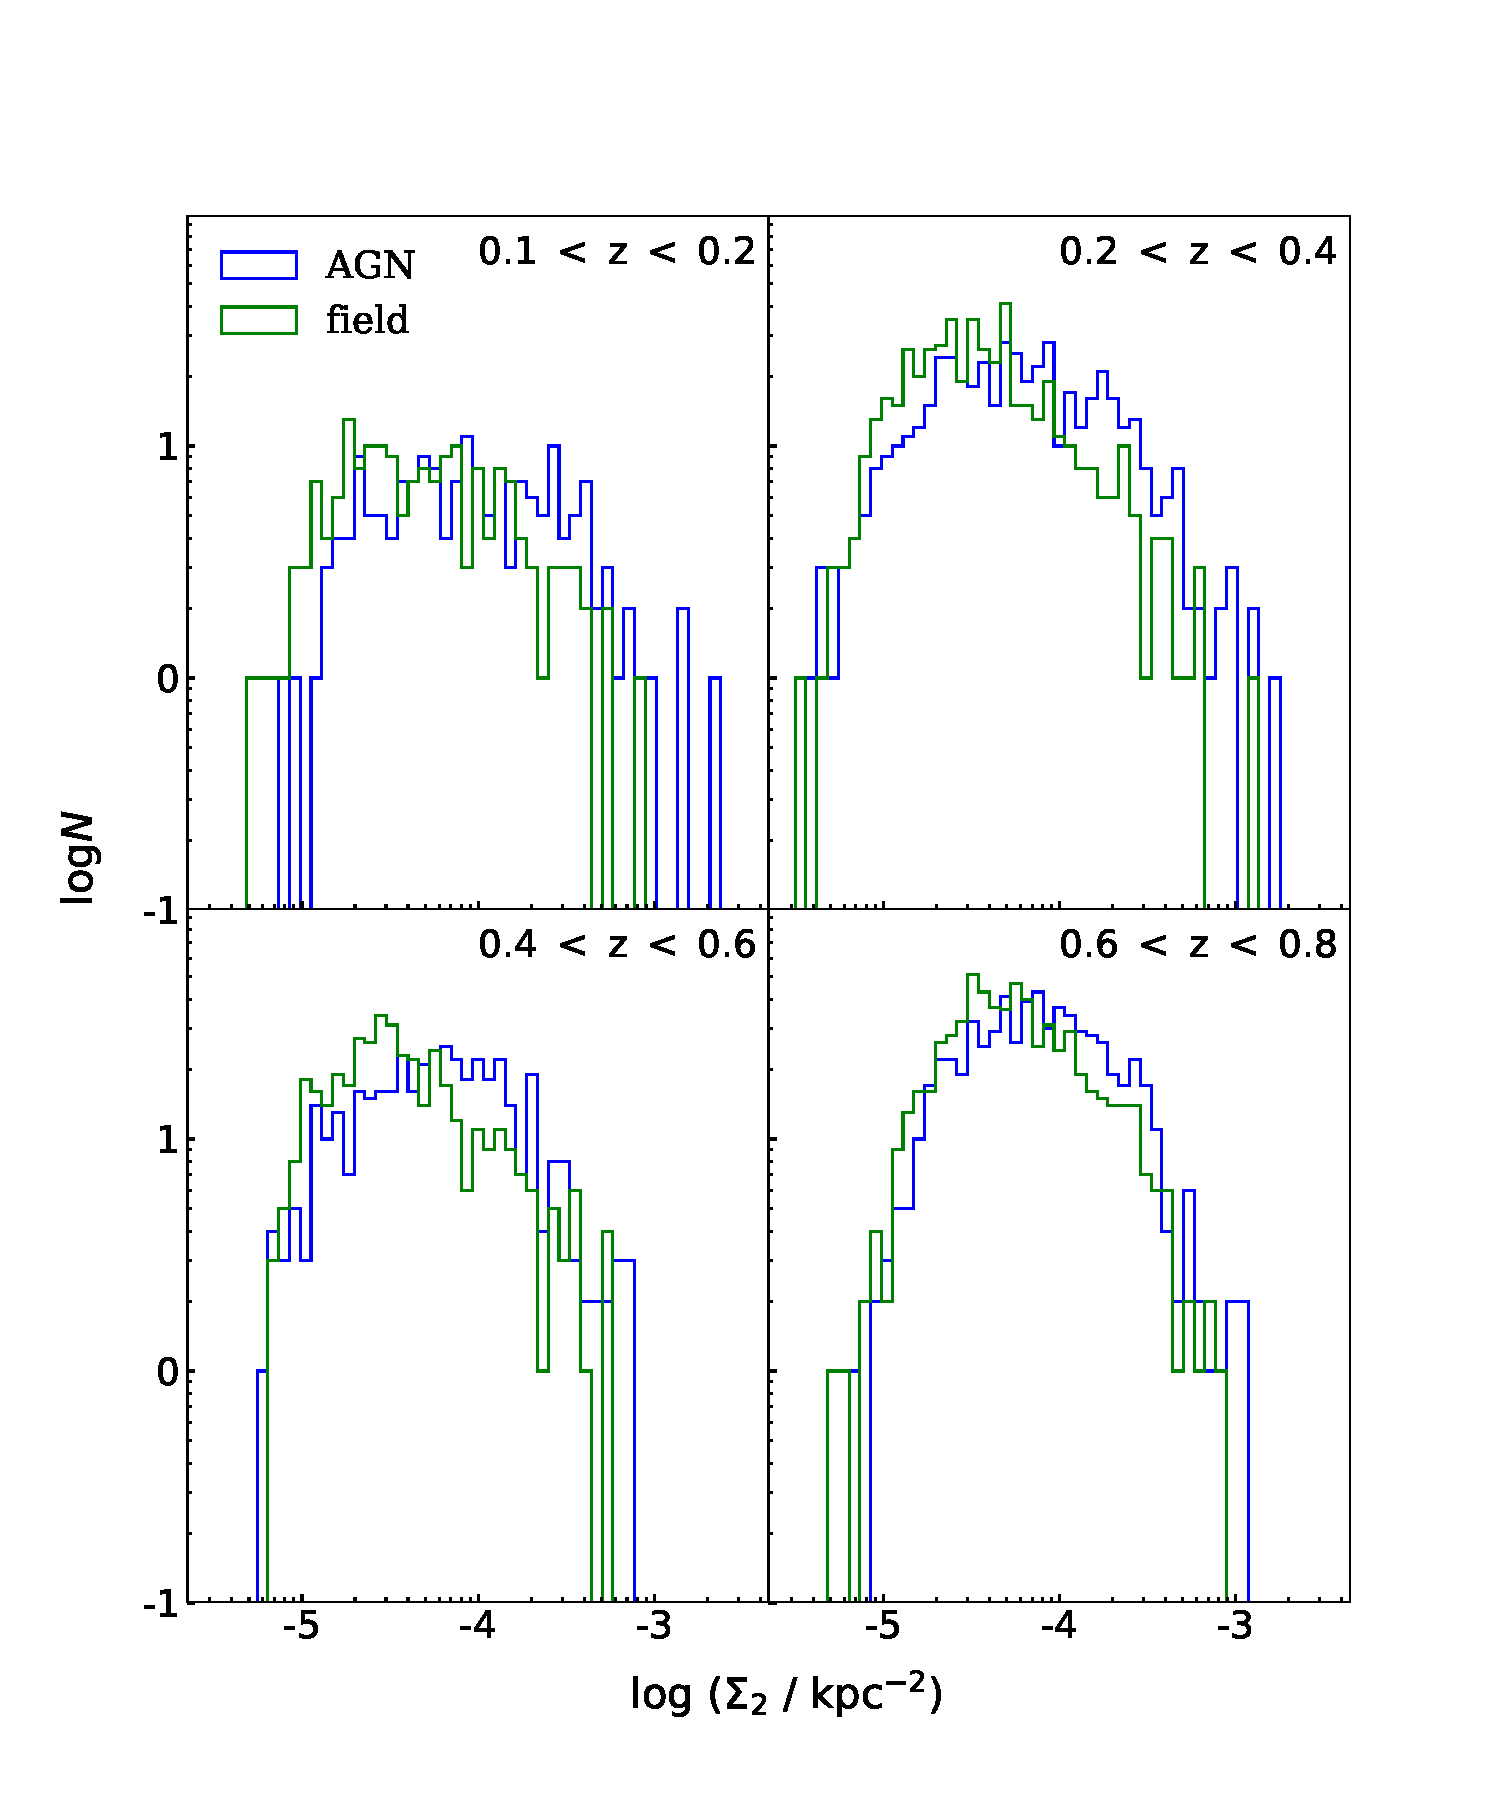
\includegraphics[width=0.6\columnwidth]{plots_chp2/random_env_2_histogram.pdf}
   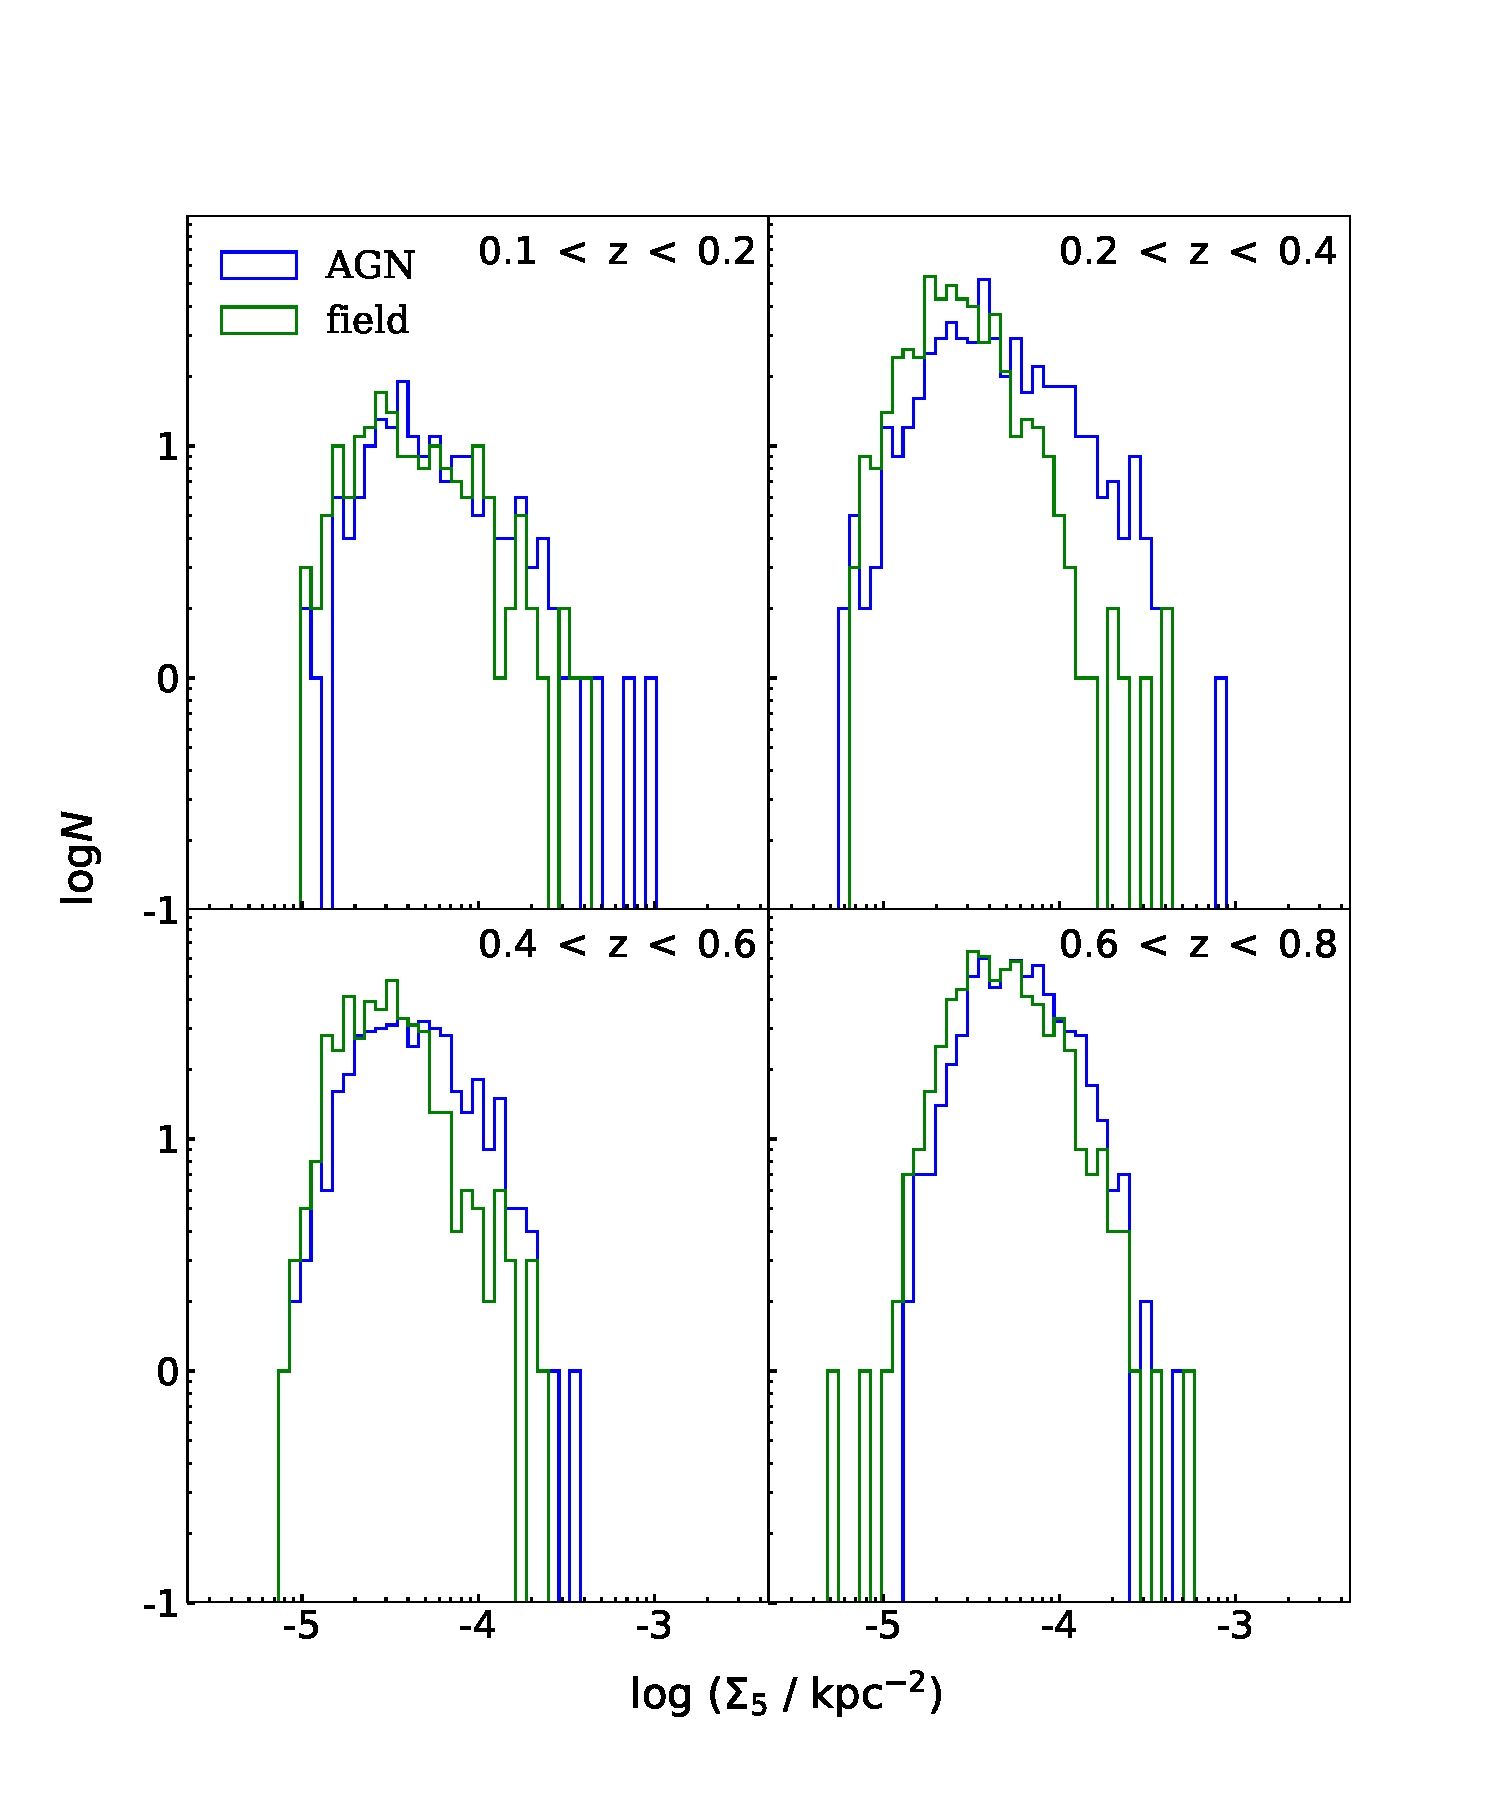
\includegraphics[width=0.6\columnwidth]{plots_chp2/random_env_5_histogram.pdf}
   \caption[Sample (i): $\Sigma_2$ and $\Sigma_5$ histograms]{Distributions of $\Sigma_2$ ($left$) and $\Sigma_5$ ($right$) of AGN and redshift-matched field samples are shown in blue and green, respectively in four redshift intervals.}
   \label{fig:random-env_L_radio_hist}
 \end{figure*}

\begin{table}
\centering
\caption[Sample (i): L$_{1.4}$-bin KS-test results]{$L_{1.4}$-bin KS-test results for control sample (i): redshift-matched.}
\label{table:sample1b}
\begin{tabular}{ c | c c c }
\hline \hline
  & Redshift Interval & $D$ & $p$ \\
  & & & \\
  \hline
   $\frac{\Sigma_{2,{\rm AGN}}}{\Sigma_{2,{\rm field}}}$ 				& 0.1 $< z <$ 0.2  &	0.242  &  $1.4\e{-5}$ \\	
   						 	& 0.2 $< z <$ 0.4  &	0.248  &  $1.5\e{-14}$ \\	
   							& 0.4 $< z <$ 0.6  & 	0.259  &  $7.3\e{-14}$ \\	
   							& 0.6 $< z <$ 0.8  &  0.156  &  $1.0\e{-7}$ \\	
  \hline
  $\frac{\Sigma_{5,{\rm AGN}}}{\Sigma_{5,{\rm field}}}$ 				& 0.1 $< z <$ 0.2  &	0.164  &  $9.8\e{-3}$ \\	
   							& 0.2 $< z <$ 0.4  & 	0.276  &  $8.3\e{-18}$ \\	
   							& 0.4 $< z <$ 0.6  & 	0.231  &  $3.8\e{-11}$ \\ 	
   							& 0.6 $< z <$ 0.8  &  0.140  &  $2.7\e{-6}$ \\	
  \hline
  \end{tabular}
\end{table}

First, we compare the relative density between the AGN and the control sample matched in redshift only. We find that the mean relative density is $>1$ in every redshift interval at $>3\sigma$ significance. In terms of the absolute overdensity, we find that the environments of AGN significantly exceed those of non-AGN (Fig.~\ref{fig:random-env_L-radio}). In terms of $\Sigma_2$ and $\Sigma_5,$ there is a good consistency between the AGN and field samples (Fig. \ref{fig:random-env_L_radio_hist}). 

However, we do not find a significant correlation between the relative environmental density at the radio luminosity of the AGN using a Spearman's rank correlation test $p$-values (Table~\ref{table:correlation_parameters}) pointing to an absence of correlation between $L_{1.4}$ and radio AGN environment density. 

The KS-tests, presented in Table~\ref{table:sample1b}, show that the environments of the AGN are statistically different to those of redshift-matched control samples. However, by only matching the AGN and control samples in terms of redshift we are neglecting the known dependence of radio luminosity on host galaxy mass \citep[e.g.][]{mclure2004,WilliamsRottgering2015}, and possibly colour. We, therefore, investigate this in the following sections. 

\subsubsection{Redshift and $K-$band magnitude-matched Control Sample}

\begin{figure*}
\hspace*{-50pt}
  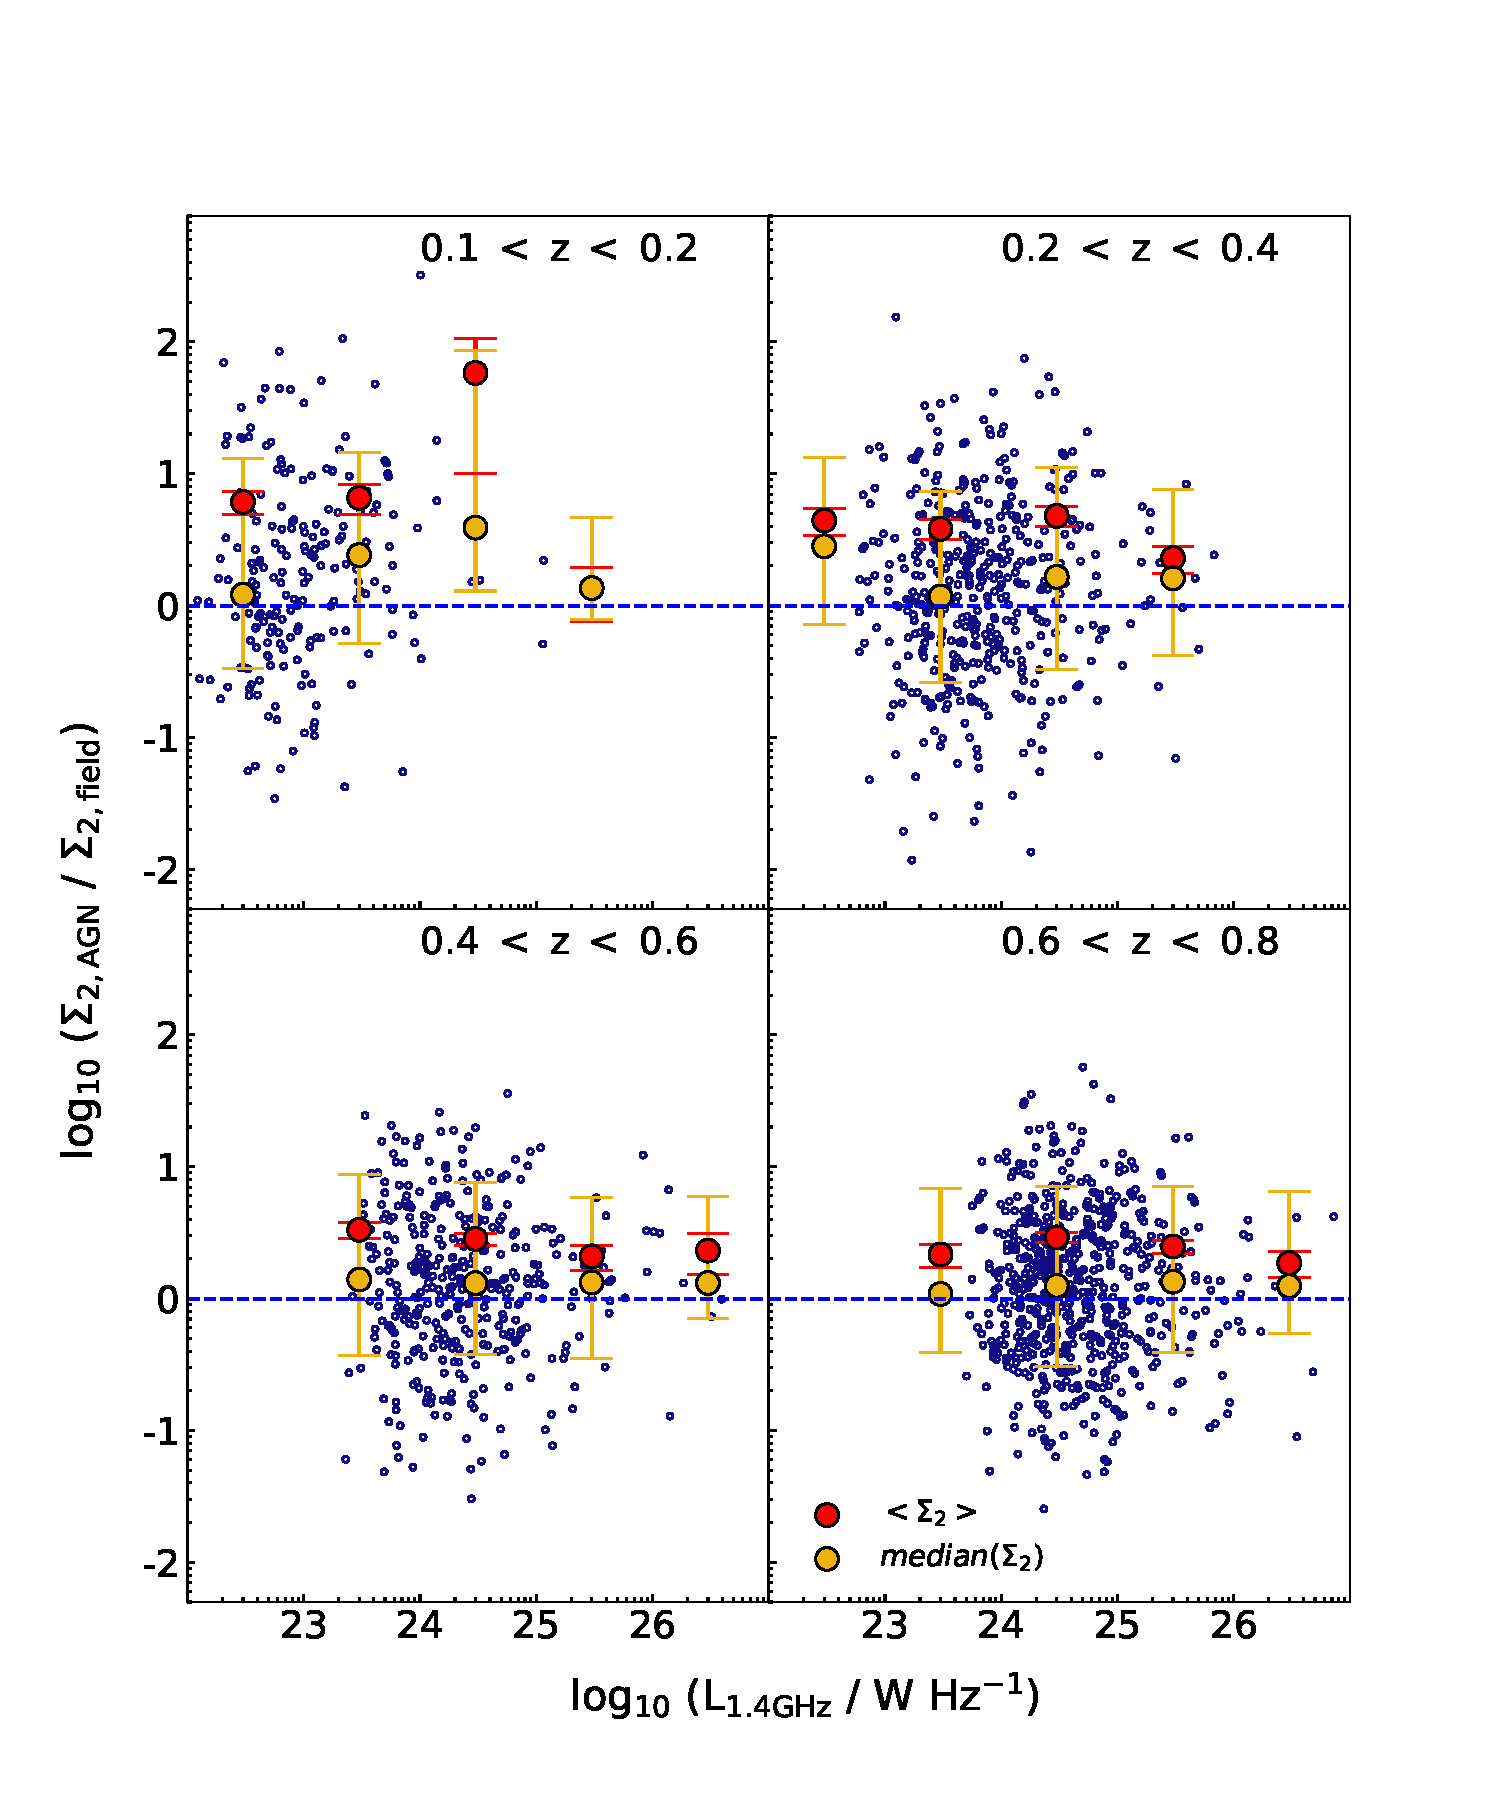
\includegraphics[width=0.6\columnwidth]{plots_chp2/env_L_radio_binned_errs_2_control.pdf}
  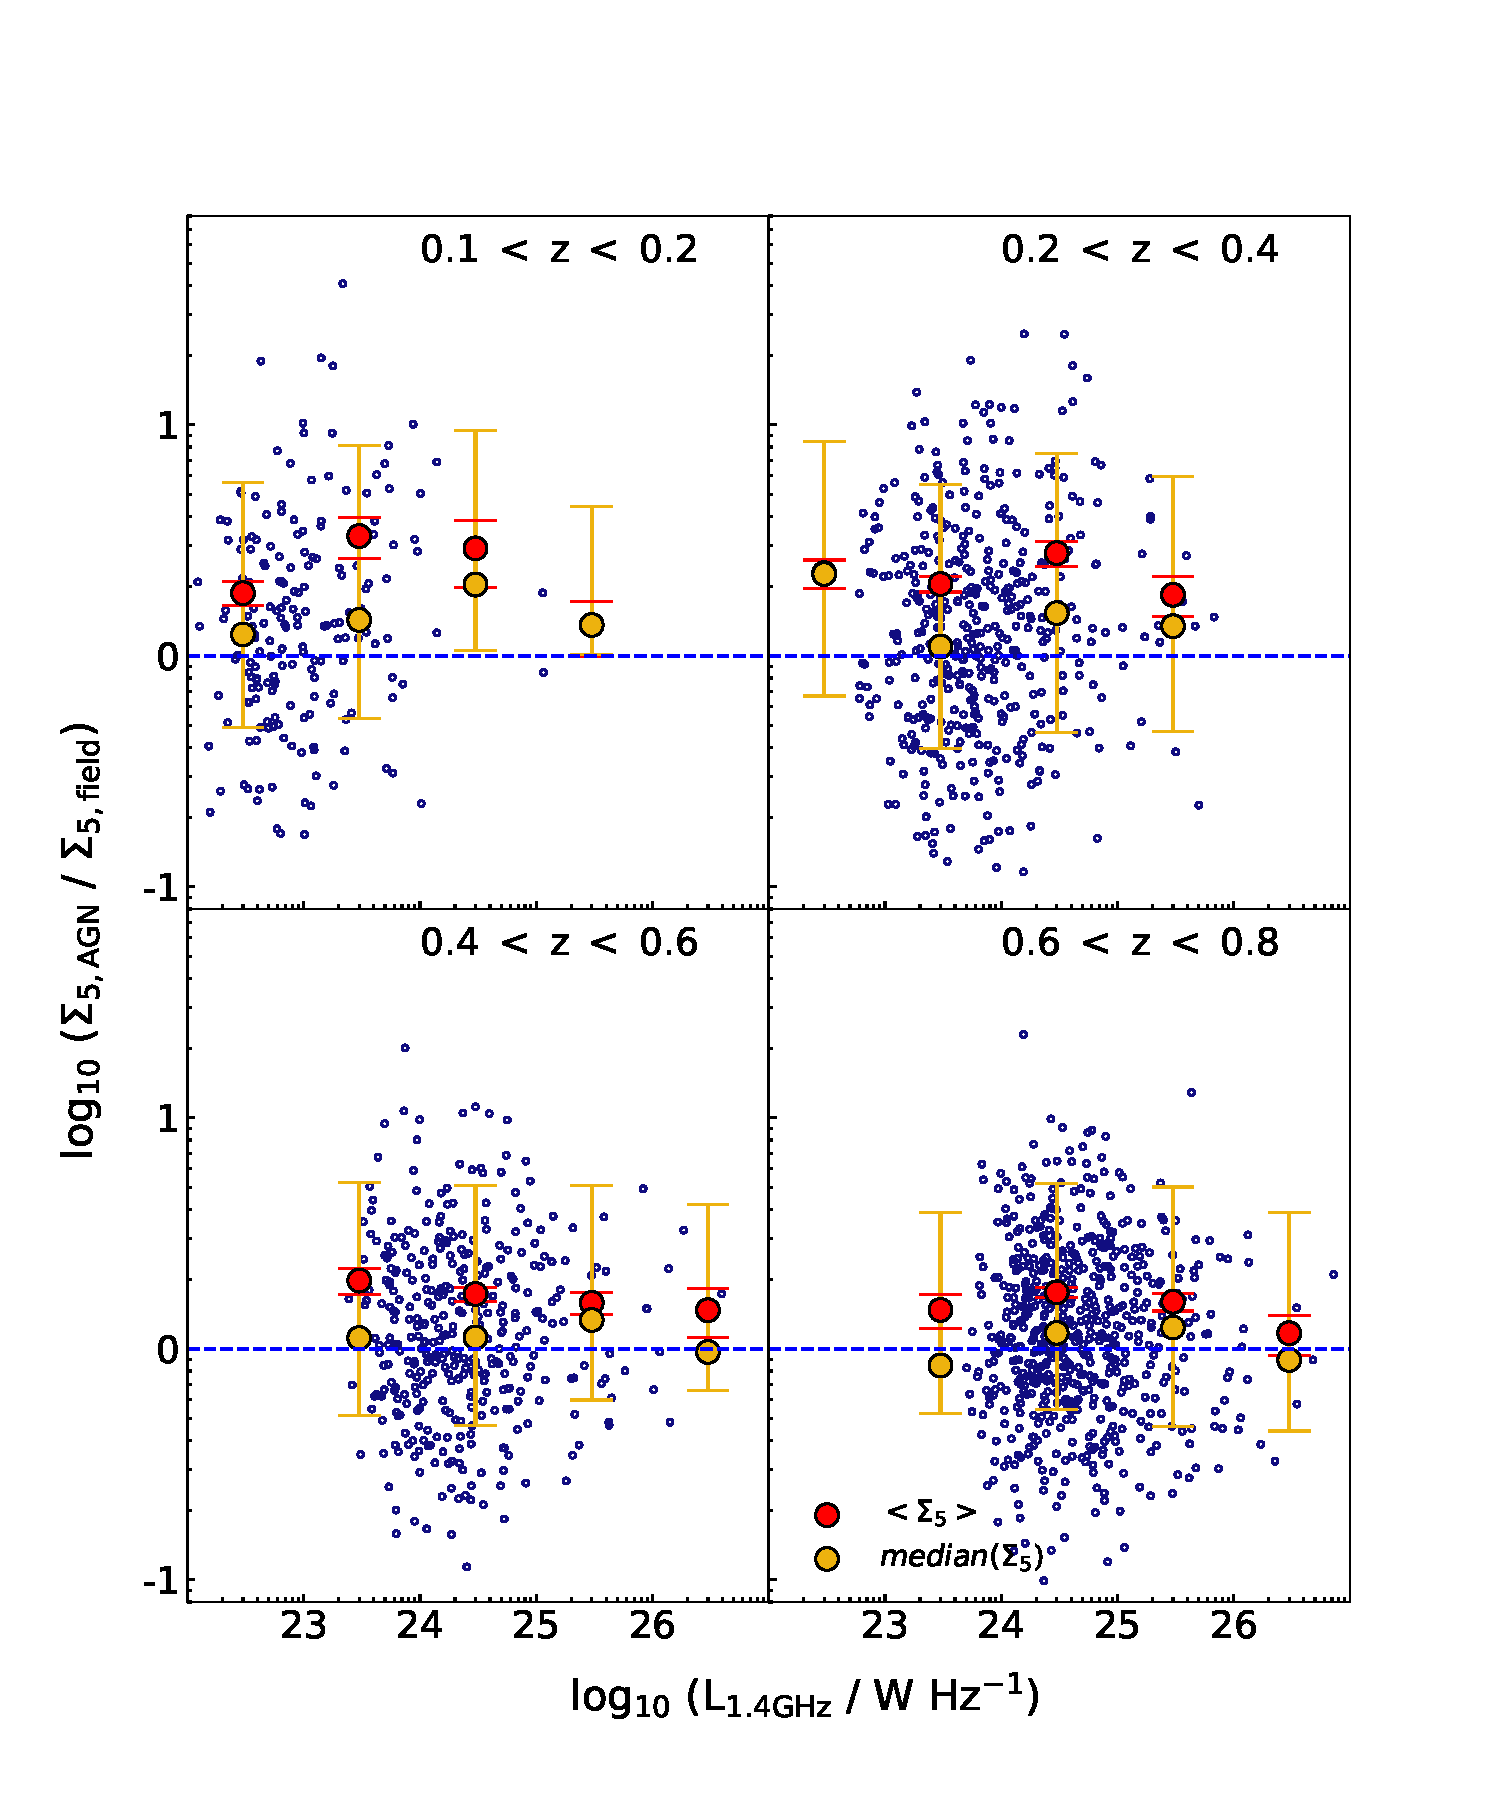
\includegraphics[width=0.6\columnwidth]{plots_chp2/env_L_radio_binned_errs_5_control.pdf}
  \caption[Sample (ii): Mean and median surface densities, $\Sigma_{2,\rm{R}}$ and $\Sigma_{5,\rm{R}}$ in $L_{1.4}$ bins.]{Same as Fig.~\ref{fig:random-env_L-radio} but for the redshift and $K-$band magnitude matched AGN and field galaxies as a function of $L_{1.4}$.}
  \label{fig:control-env_L_radio}
\end{figure*}

\begin{figure*}
\hspace*{-50pt}
   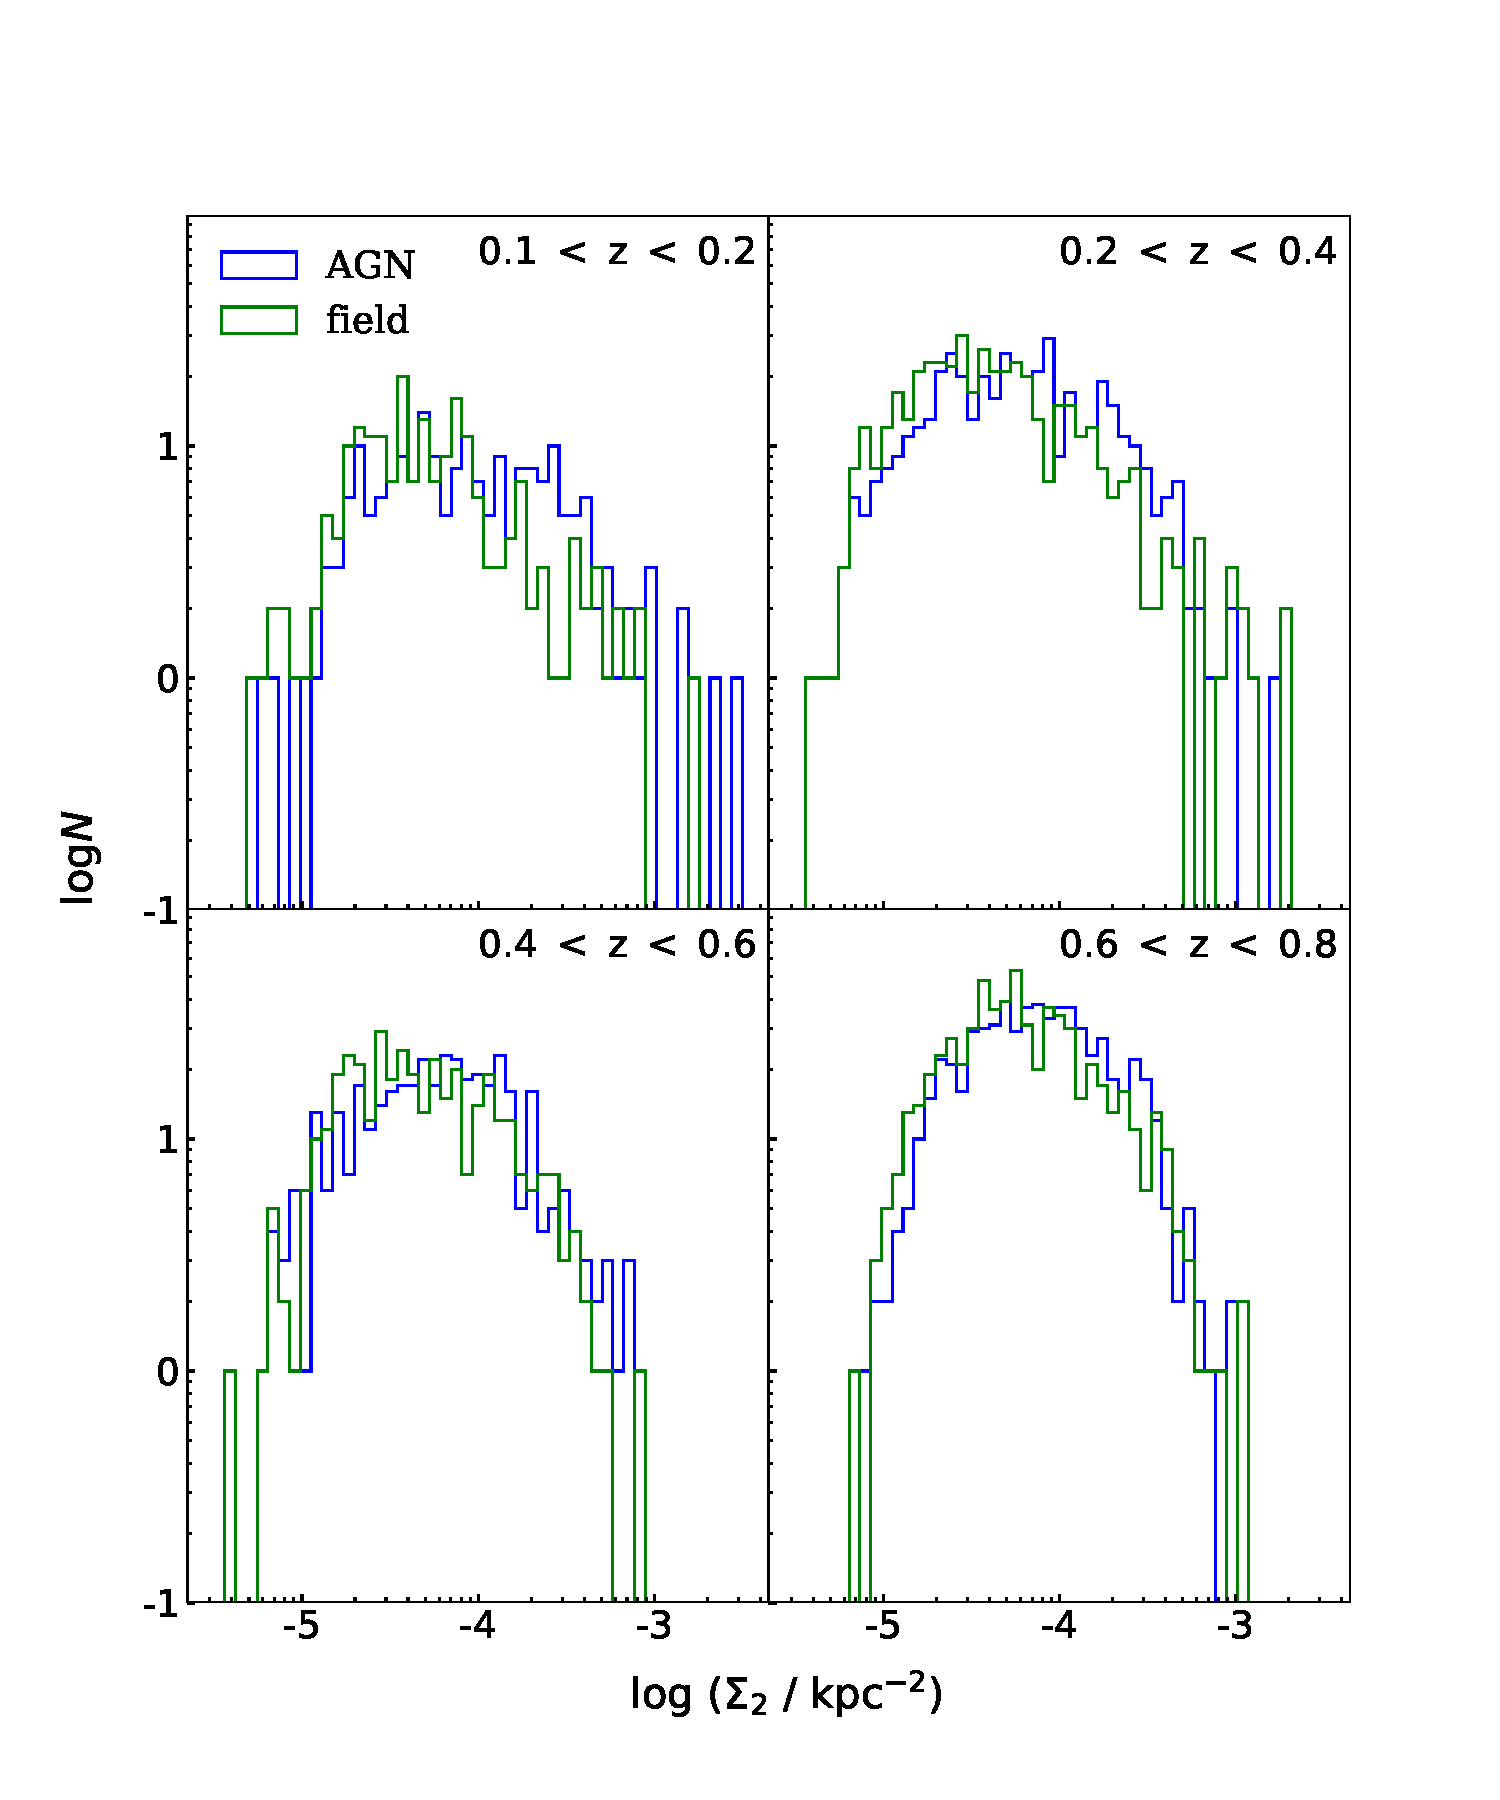
\includegraphics[width=0.6\columnwidth]{plots_chp2/control_env_2_histogram.pdf}
   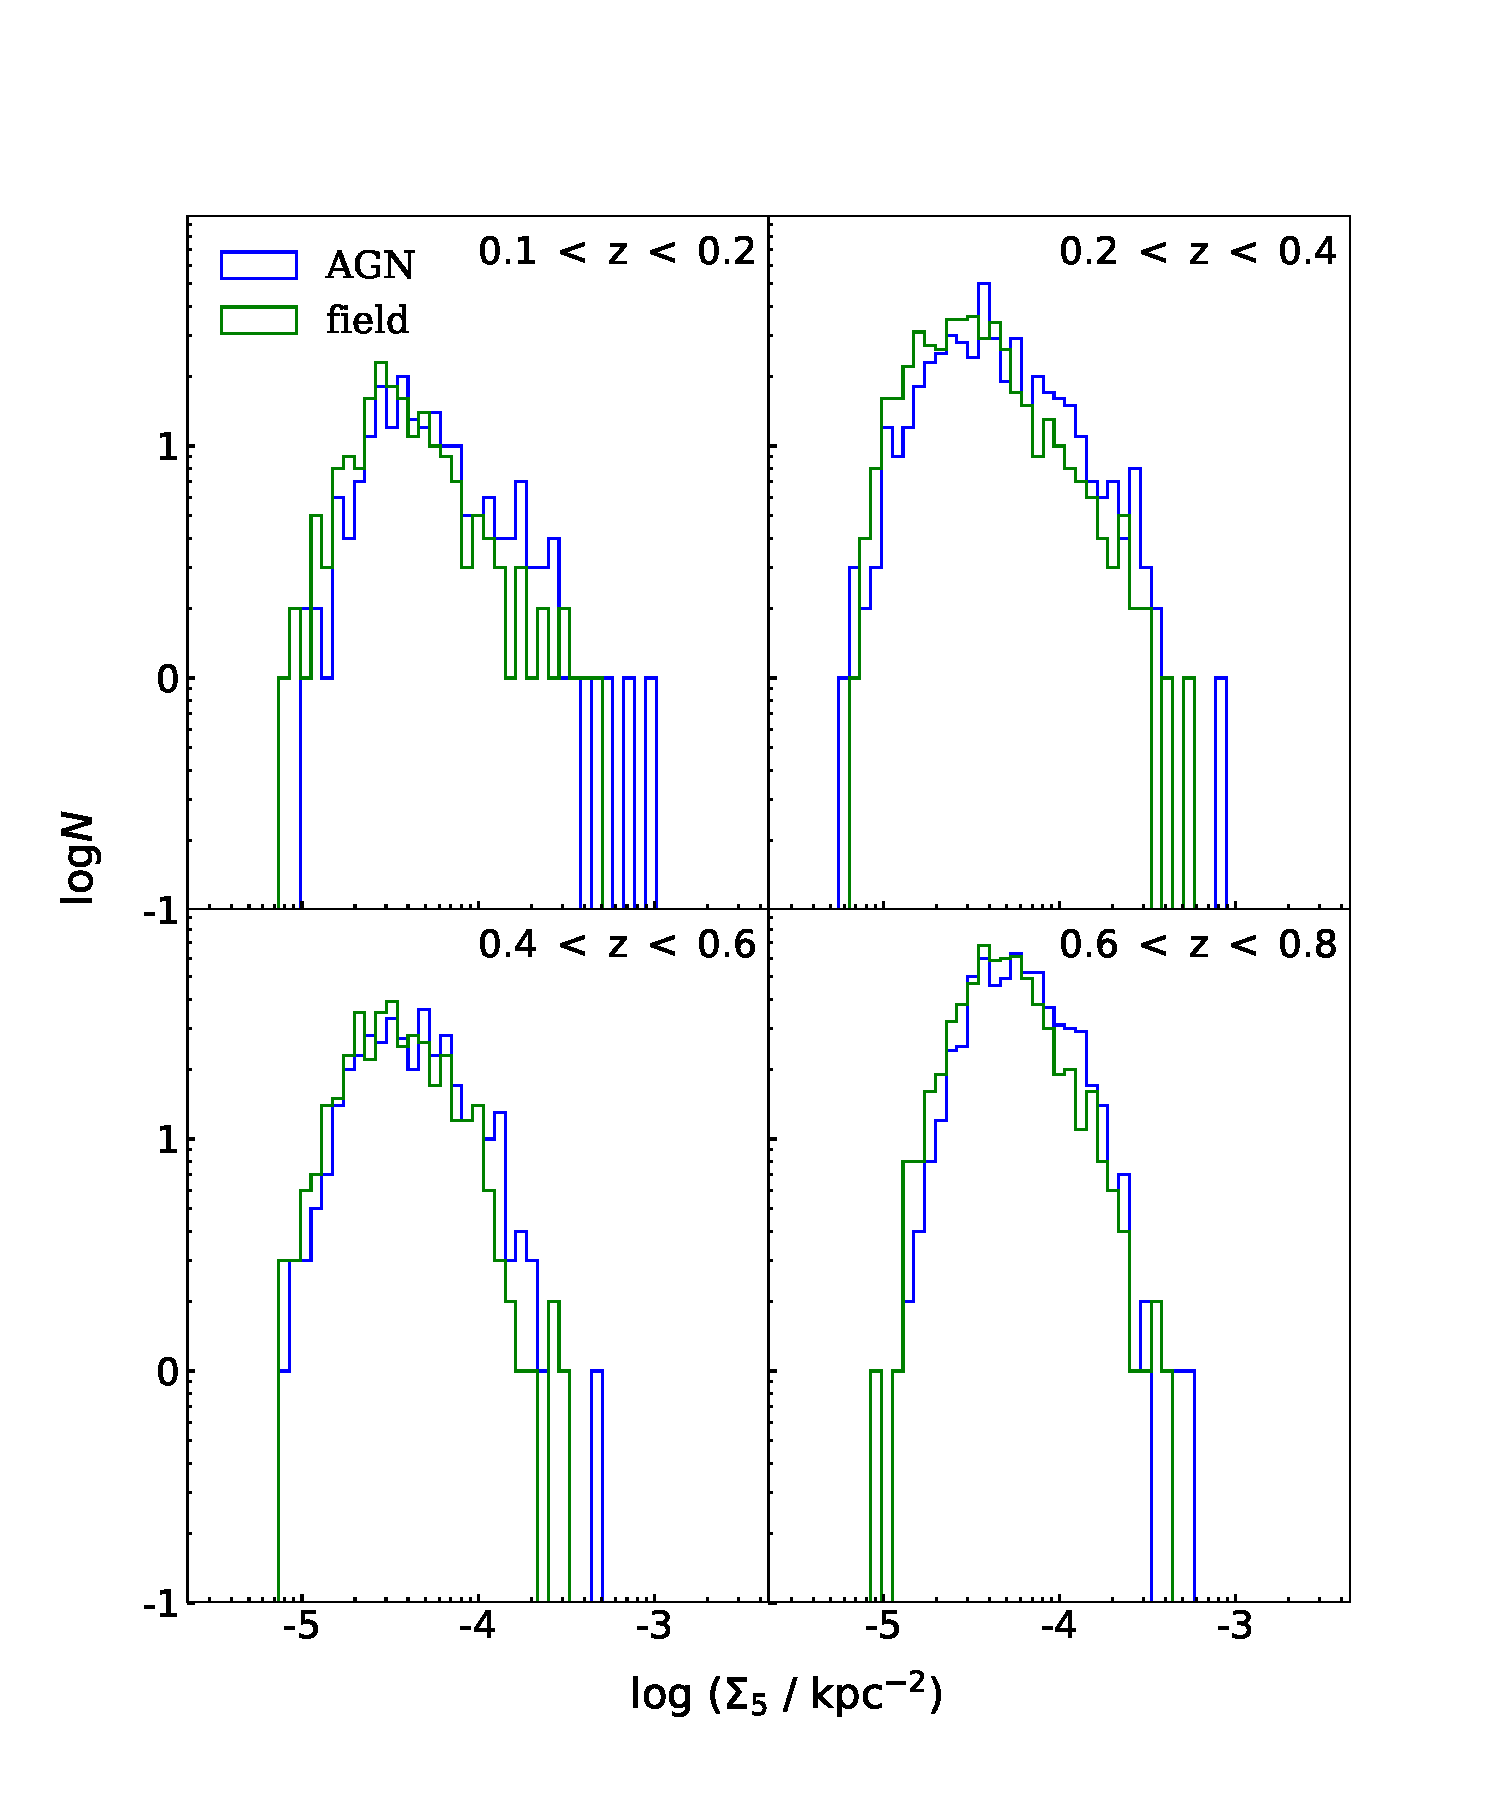
\includegraphics[width=0.6\columnwidth]{plots_chp2/control_env_5_histogram.pdf}
   \caption[Sample (ii): $\Sigma_2$ and $\Sigma_5$ histograms]{Same as Fig.~\ref{fig:random-env_L_radio_hist} except for the redshift and $K-$band magnitude matched AGN and field galaxies.}
   \label{fig:control-env_L_radio_hist}
 \end{figure*}

In sample (ii), the AGN and control sources are matched in redshift and $K-$band magnitude, which is related to the stellar mass of the galaxy. As depicted in Fig.~\ref{fig:K-z-supercontrol}, the $z$ and $K-$band magnitude source matching is successful given the overlapping distributions in AGN and control distributions.

Correlation test parameters for the density-$L_{1.4}$ relation of the redshift and $K-$band magnitude matched sample are shown in Table~\ref{table:correlation_parameters}.
We find that the mean relative density is consistently $>1$ in both $\Sigma_{2,\rm{R}}$ and $\Sigma_{5,\rm{R}}$ for all redshift intervals and $L_{1.4}$ intervals, as shown by Fig. \ref{fig:control-env_L_radio}. In terms of $\Sigma_2$ and $\Sigma_5,$ there is a good consistency between the AGN and field samples (Fig. \ref{fig:control-env_L_radio_hist}). 

According to the KS-tests (Table~\ref{table:sample2b}), the control sample is drawn from a different underlying distribution to that of the AGN for both $\Sigma_{2,\rm{R}}$ and $\Sigma_{5,\rm{R}}$, in all redshift bins. However, we find that the significance of this is reduced compared to the redshift-only control sample, suggesting that the $K-$band magnitude, or more physically, the stellar mass plays a crucial role in the measurement of the environmental density. This is expected as a multitude of studies have shown that more massive galaxies are more highly clustered, and thus reside in higher mass dark matter haloes \citep[e.g.][]{Norberg2002,Zehavi2011}. Given that higher mass haloes tend to all contain a high number of satellites \citep{mccracken2015,Hatfield2016}, this finding is in agreement with the accepted view offered by hierarchical galaxy formation models.

\begin{table}
\centering
\caption[Sample (ii): L$_{1.4}$-bin KS-test results]{$L_{1.4}$-bin KS-test results for control sample (ii): redshift and $K-$band magnitude-matched field.}
\label{table:sample2b}
\begin{tabular}{c | c c c}
\hline \hline
  & Redshift Interval & $D$ & $p$ \\
  & & & \\
  \hline
   	$\frac{\Sigma_{2,{\rm AGN}}}{\Sigma_{2,{\rm field}}}$	& 0.1 $< z <$ 0.2 	&	0.256  &  $1.4\e{-6}$ \\
   							& 0.2 $< z <$ 0.4 	& 	0.164  &  $2.3\e{-6}$ \\
   							& 0.4 $< z <$ 0.6 	&	0.157  &  $3.7\e{-5}$ \\
   							& 0.6 $< z <$ 0.8 	&	0.116  &  $2.2\e{-4}$ \\
  \hline
   $\frac{\Sigma_{5,{\rm AGN}}}{\Sigma_{5,{\rm field}}}$	& 0.1 $< z <$ 0.2 	& 	0.175  &  $3.1\e{-3}$ \\
   							& 0.2 $< z <$ 0.4 	& 	0.144  &  $5.4\e{-5}$ \\
   							& 0.4 $< z <$ 0.6 	& 	0.124  &  $2.4\e{-3}$ \\
   							& 0.6 $< z <$ 0.8 	& 	0.114  &  $3.0\e{-4}$ \\               
  \hline
  \end{tabular}
\end{table}

\subsubsection{Redshift, $K-$band magnitude and ($g-K$)-matched Control Sample}

\begin{figure*}
\hspace*{-50pt}
  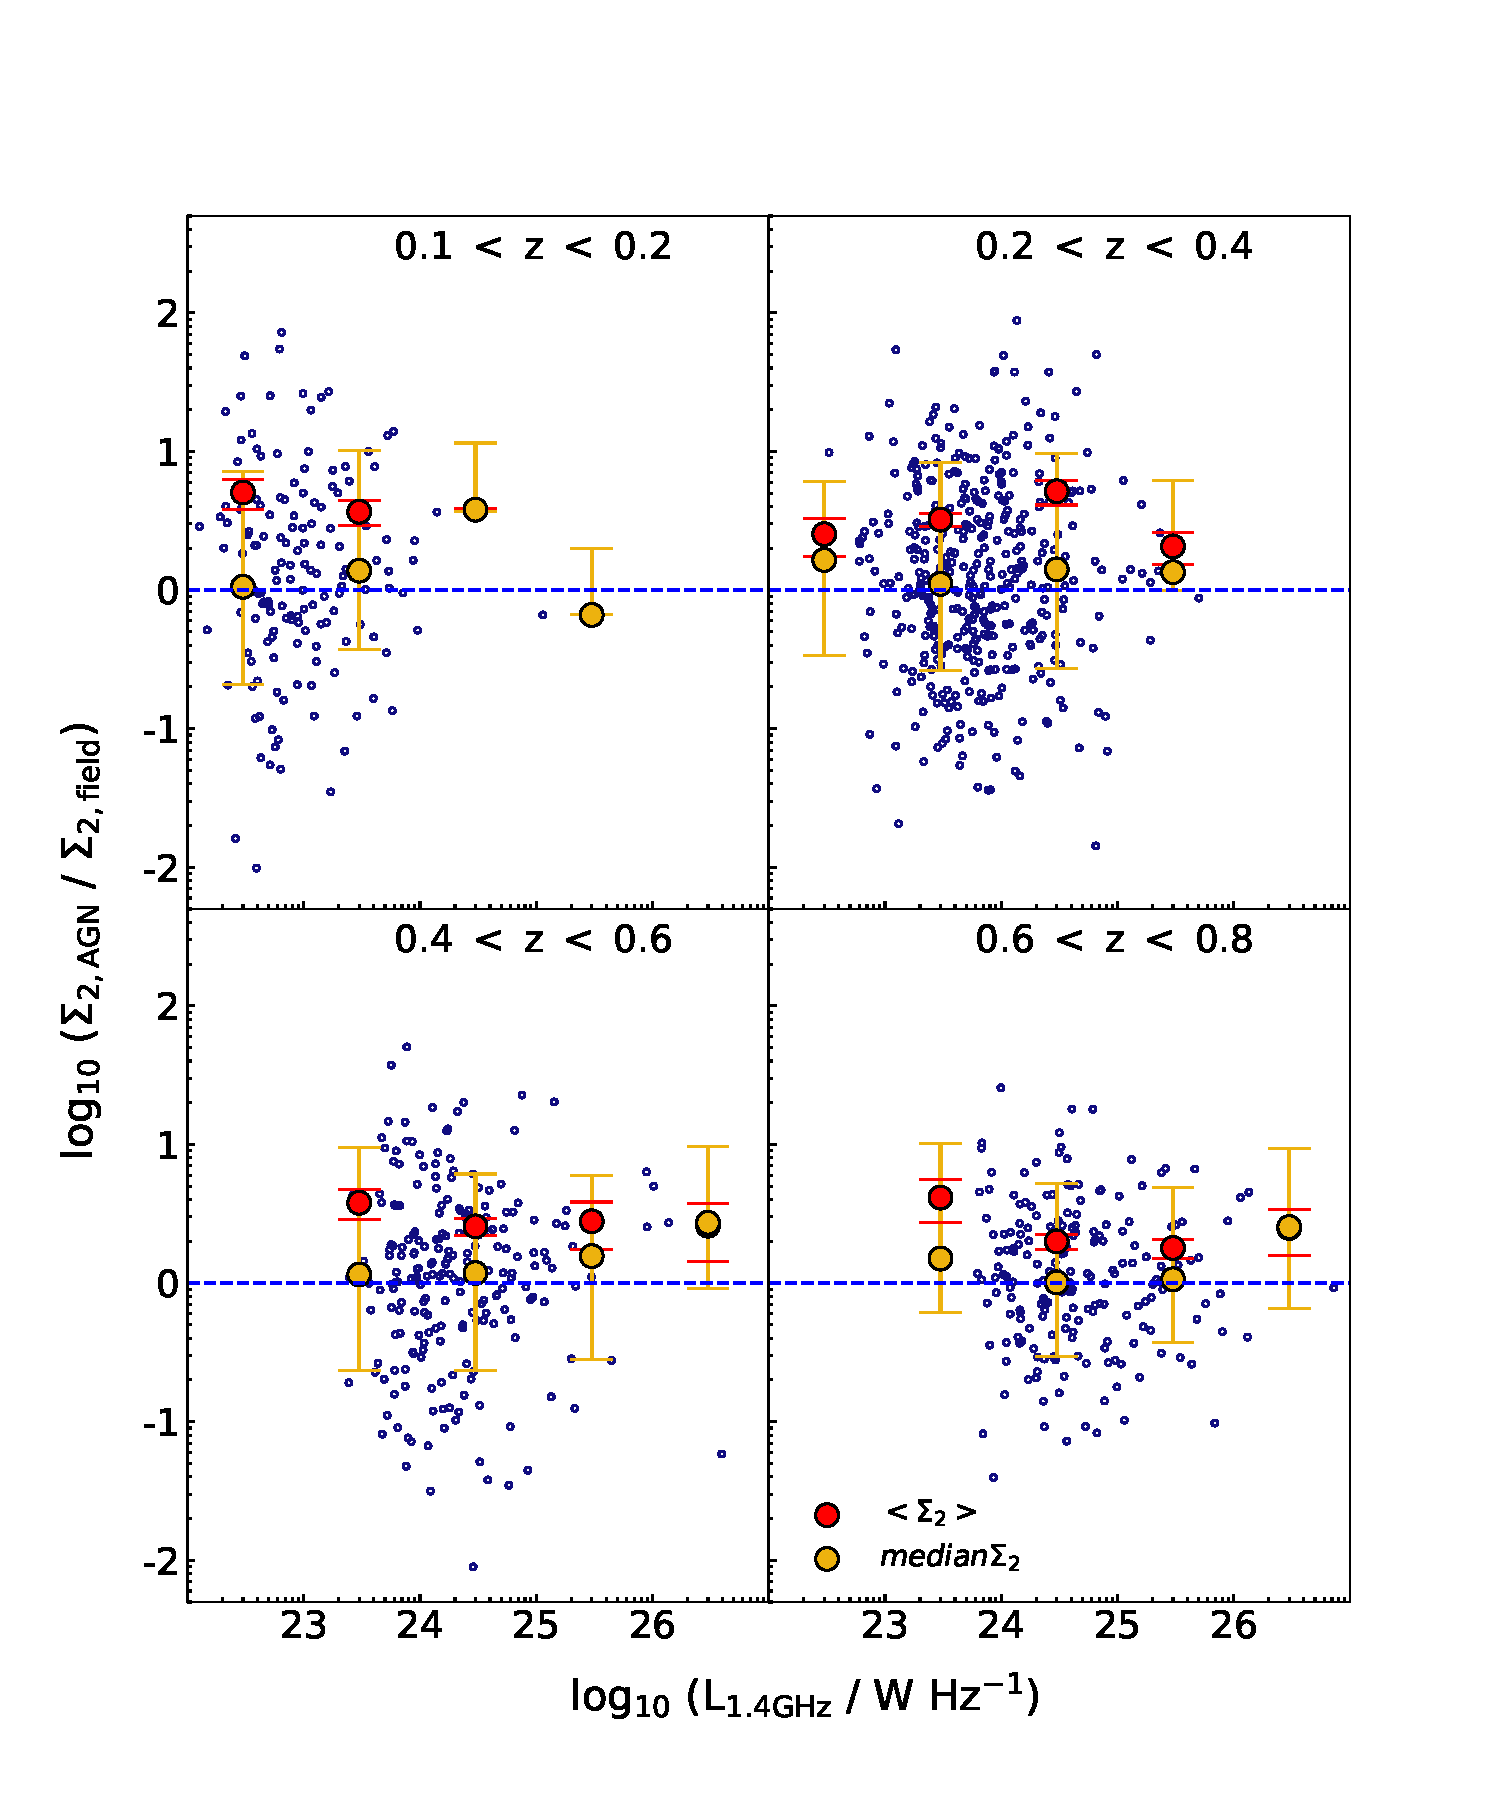
\includegraphics[width=0.6\columnwidth]{plots_chp2/env_L_radio_binned_errs_2_super_control.pdf}
  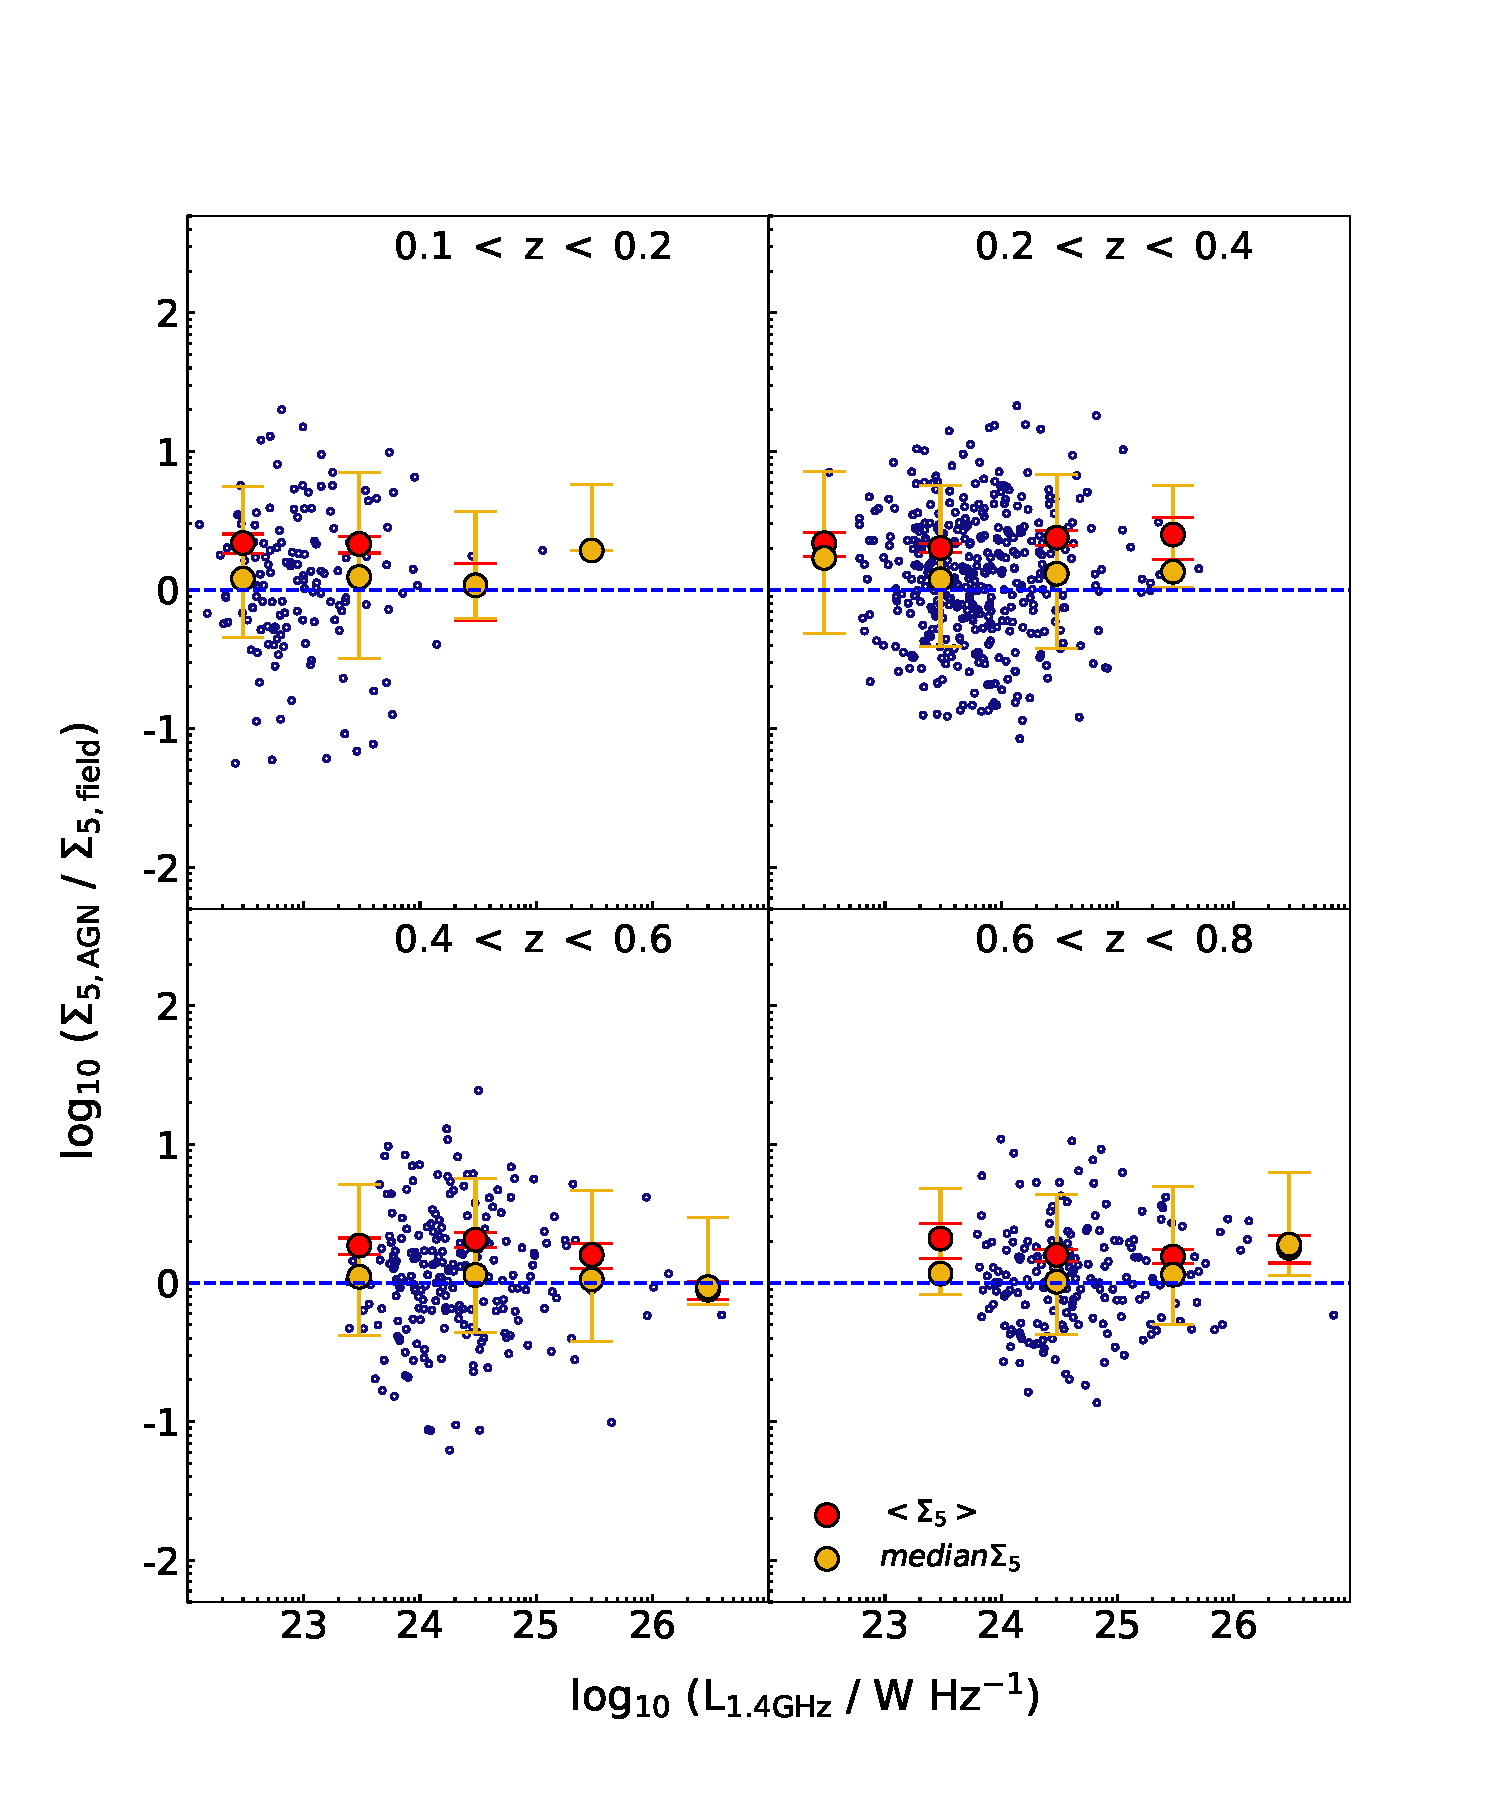
\includegraphics[width=0.6\columnwidth]{plots_chp2/env_L_radio_binned_errs_5_super_control.pdf}
  \caption[Sample (iii): Mean and median surface densities, $\Sigma_{2,\rm{R}}$ and $\Sigma_{5,\rm{R}},$ in $L_{1.4}$ bins.]{Same as Fig.~\ref{fig:random-env_L-radio} but for the redshift, $K-$band magnitude and ($g-K$)-colour matched AGN and field galaxies as a function of $L_{1.4}$. }
  \label{fig:supercontrol-env_L-radio}
\end{figure*}

\begin{figure*}
\centering
 \subfloat[$\Sigma_2$ distributions for AGN and control samples]{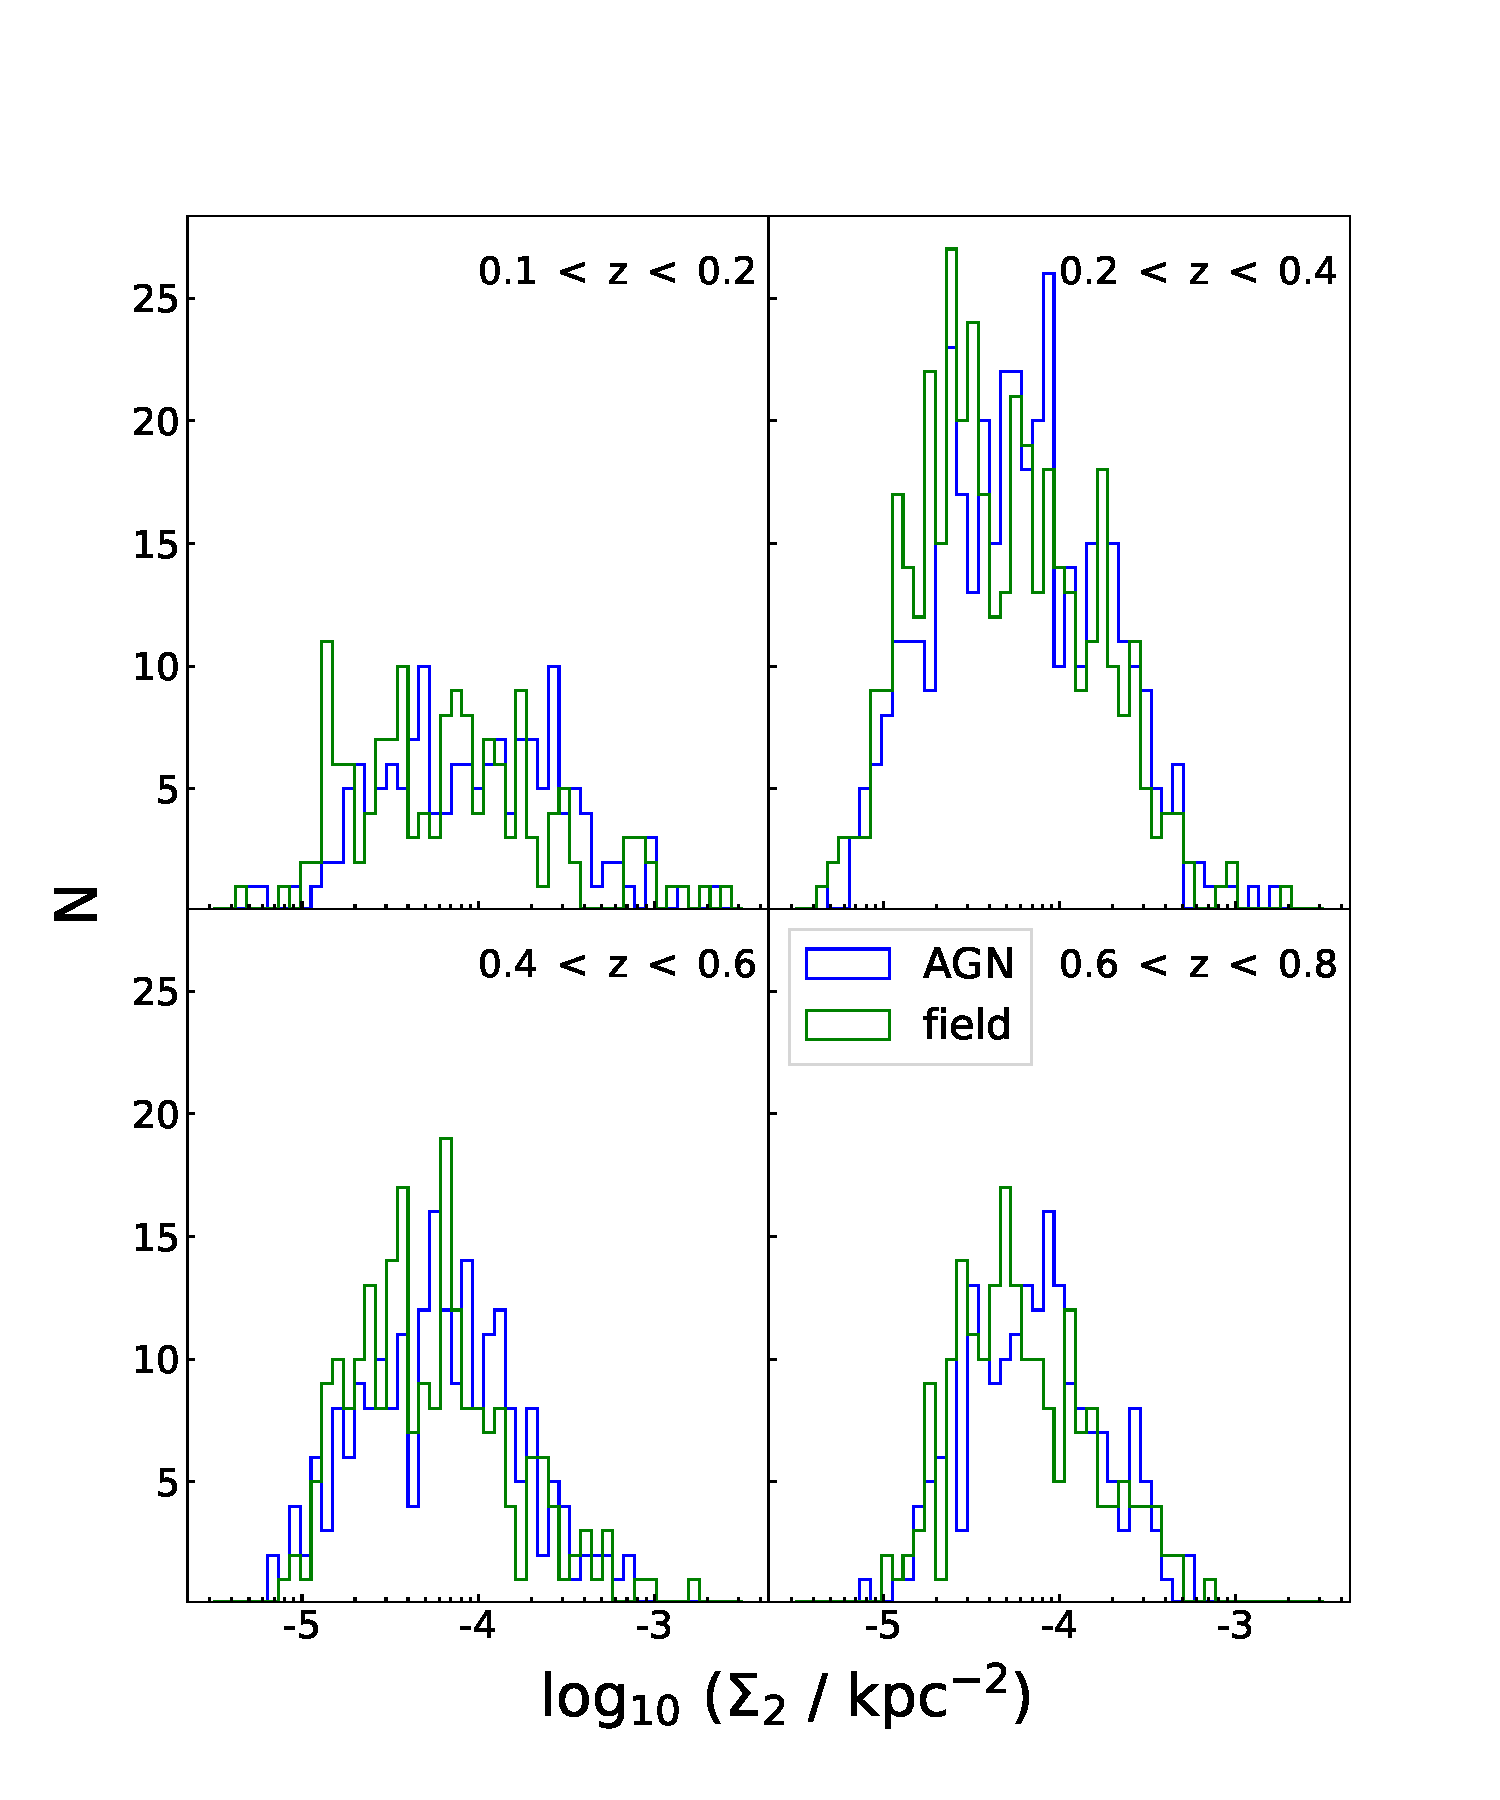
\includegraphics[width=0.5\columnwidth]{plots_chp2/super_env_2_histogram.pdf}}
 \subfloat[$\Sigma_5$ distributions for AGN and control samples]{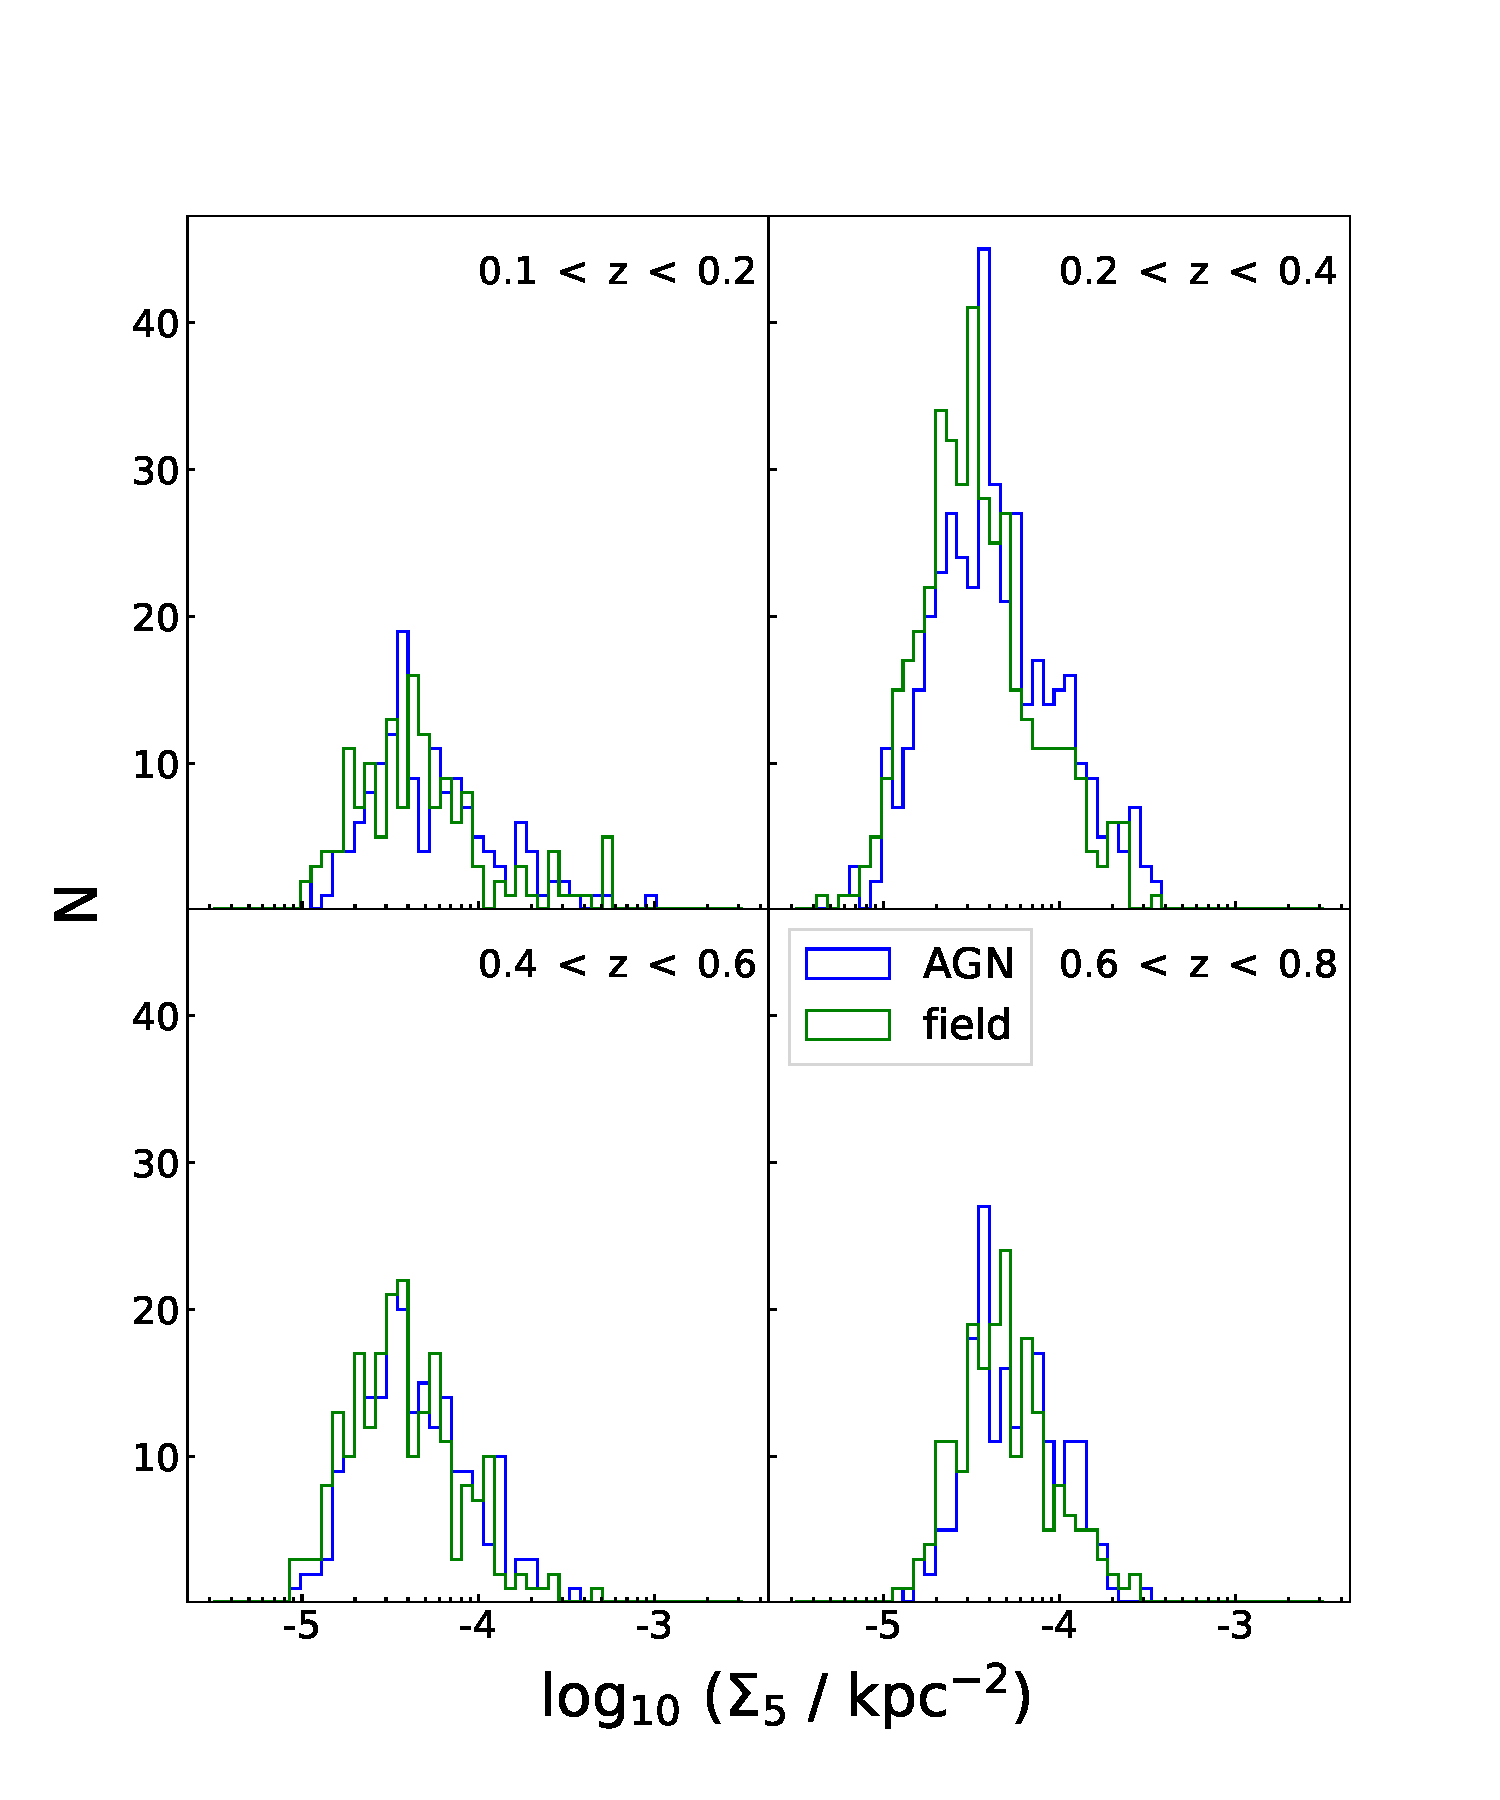
\includegraphics[width=0.5\columnwidth]{plots_chp2/super_env_5_histogram.pdf}}\\
 \subfloat[$\Sigma_{2,\rm{R}}$ distributions for AGN and control samples]{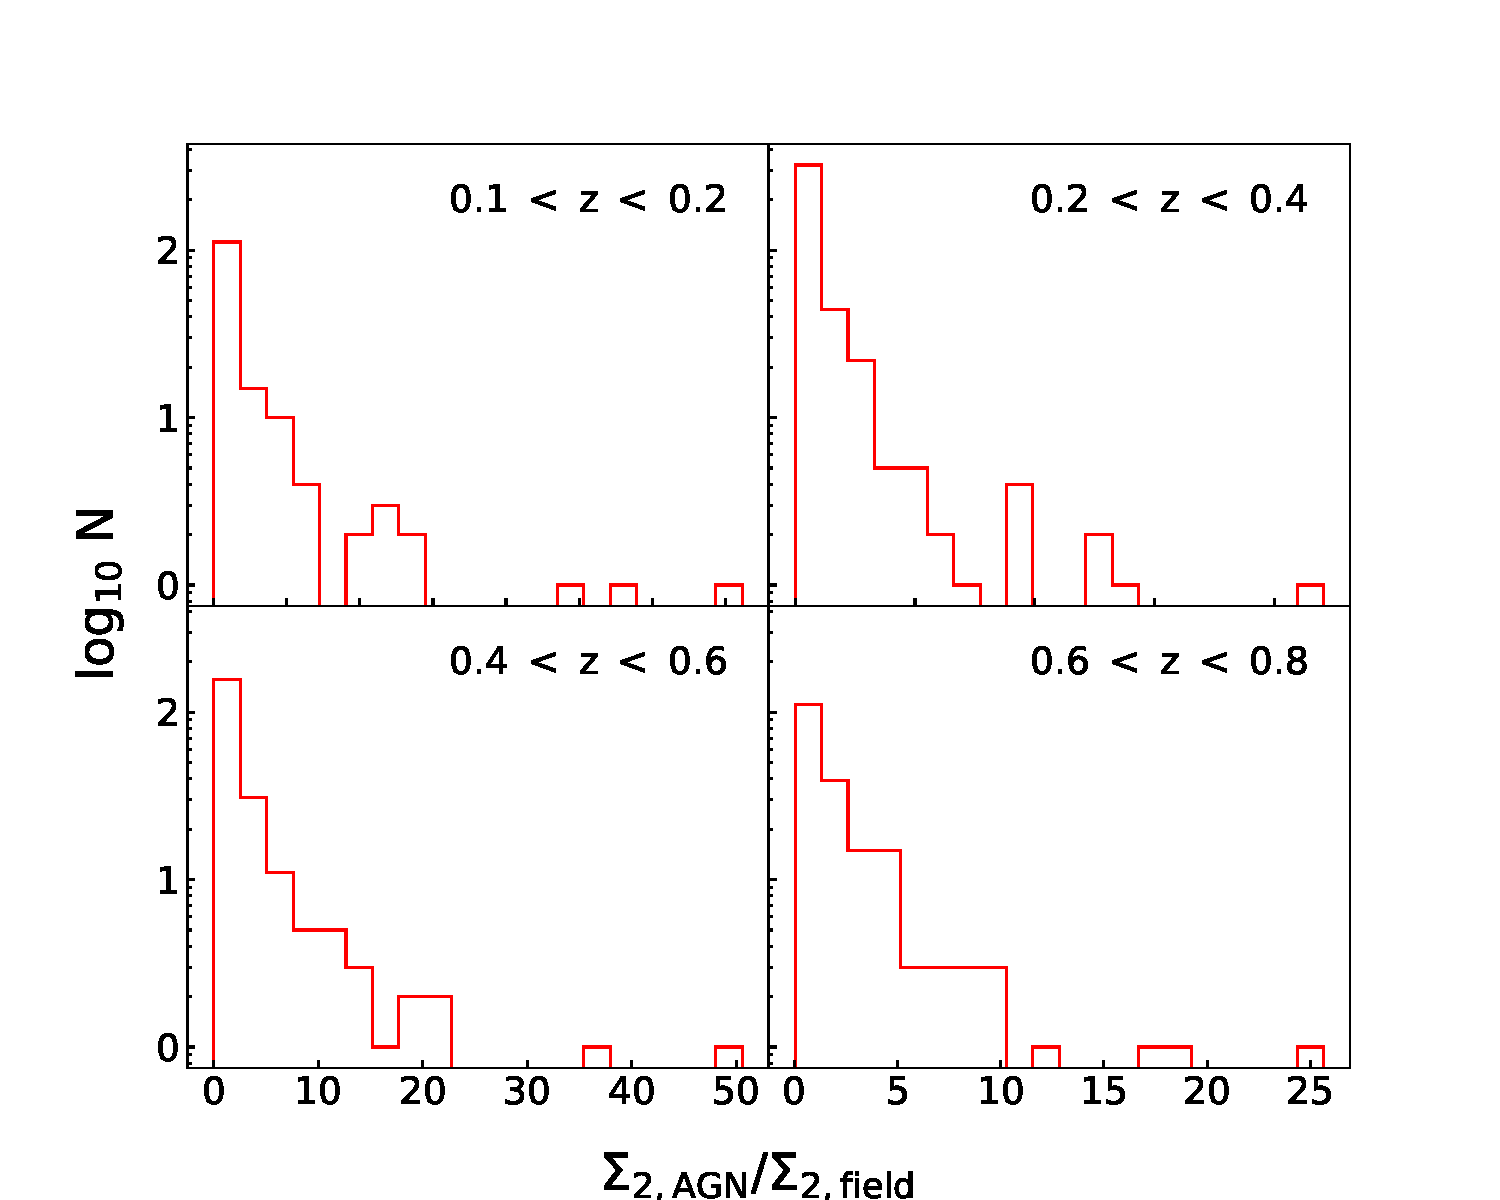
\includegraphics[width=0.5\columnwidth]{plots_chp2/super_env_2_ratio_histogram.pdf}}
 \subfloat[$\Sigma_{5,\rm{R}}$ distributions for AGN and control samples]{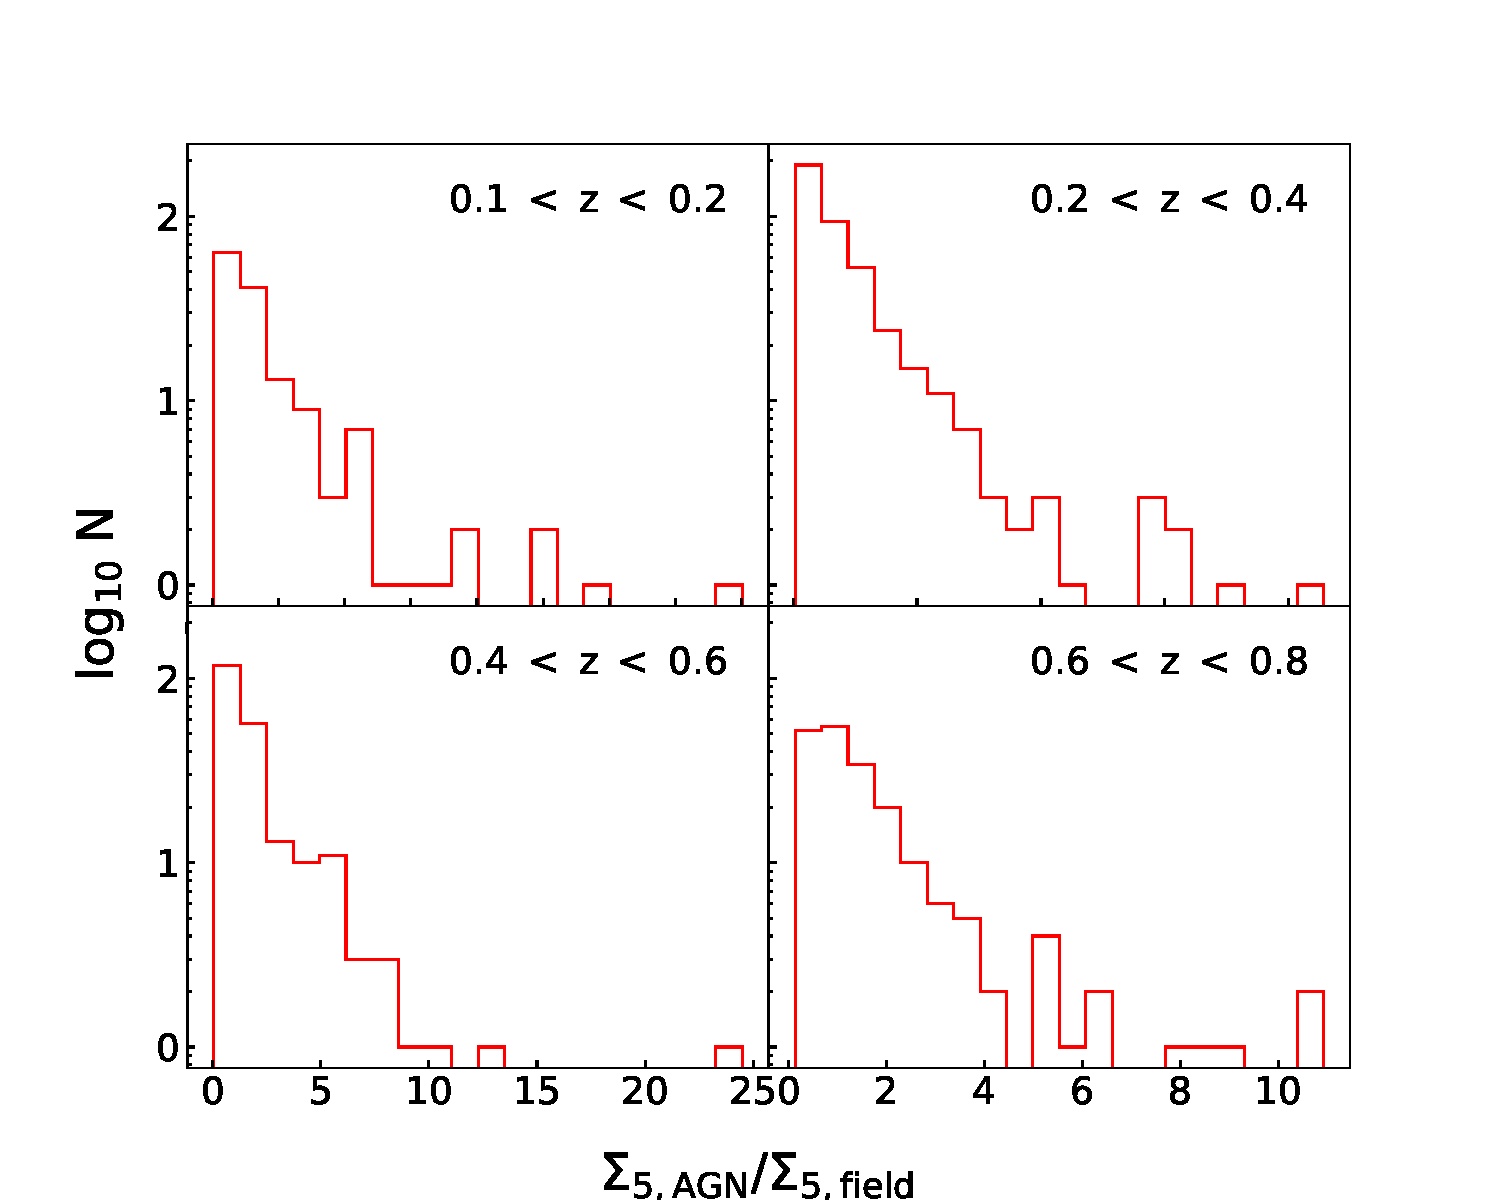
\includegraphics[width=0.5\columnwidth]{plots_chp2/super_env_5_ratio_histogram.pdf}}
  \caption[Sample (iii): $\Sigma_2$ and $\Sigma_5$ histograms; $\Sigma_{2,\rm{R}}$ and $\Sigma_{5,\rm{R}}$ histograms]{Distributions of $\Sigma_2$ (kpc$^{-2}$) and $\Sigma_5$ (kpc$^{-2}$) for the AGN and redshift, $K-$band magnitude and ($g-K$)-colour matched control galaxies in panels (a) and (b). The relative density distributions i.e. $\Sigma_{2,\rm{R}}$ and $\Sigma_{5,\rm{R}},$ are also shown in panels (c) and (d).}
  \label{fig:supercontrol-env_L_radio_hist}
\end{figure*}

Galaxy stellar mass and redshift, are not the only issues that may need to be considered in terms of forming a control sample. Galaxy colour may also be related to the galaxy environment \citep[e.g.][]{Madgwick2003,Zehavi2011,Wang2018}. We, therefore, attempt to control for this with sample (iii), which is a redshift, $K-$band magnitude and ($g-K$)-matched sample. Figs.~\ref{fig:K-z-supercontrol} and \ref{fig:g-K-z-supercontrol} show the distributions for the radio source and control sample. 

Fig. \ref{fig:supercontrol-env_L-radio} shows that the mean relative density is $>1$ in $\Sigma_{2,\rm{R}}$ and $\Sigma_{5,\rm{R}}$ within all redshift and $L_{1.4}$ intervals for control sample (iii). The KS-test results in Table \ref{table:sample3b} indicate that the AGN and control density distributions (both measured using $\Sigma_{2,\rm{R}}$ and $\Sigma_{5,\rm{R}}$) are inconsistent with being drawn from the same underlying distribution at the $\sim 99$ per cent level.

We also note that the the $p$-values in the KS-tests become progressively larger as we move from sample (i) to sample (iii). As expected the density distributions are most statistically different in the sample that has been matched to the radio AGN with the least number of criteria, i.e. redshift only. As the matching procedure becomes more stringent, the statistical difference between the density distributions of AGN and control galaxies becomes lower (see Tables \ref{table:sample1b}, \ref{table:sample2b} and \ref{table:sample3b}).

In Fig.~\ref{fig:supercontrol-env_L_radio_hist}, we also show the distributions of $\Sigma_{2,\rm{R}}$ and $\Sigma_{5,\rm{R}}$ for both the AGN and control sample (iii). This provides more information on the scales that the environments are being traced. For example, $10^{-5} \lesssim \Sigma_{5,\rm{R}} / $\,kpc$^{-2} \lesssim 10^{-3}$ corresponds to radii or separations ($d_N$) of $0.04 \lesssim d_N / \,$kpc $\lesssim 400$. From this we can infer that we are well within the 1-halo term regime, and are only tracing the environments of the AGN and control samples within the dark matter halo in which they reside, and not the larger scale 2-halo clustering.

\begin{table}
\centering
\caption[Sample (iii): L$_{1.4}$-bin KS-test results]{KS-test results for local AGN density compared to control galaxies (field) density in sample (iii): redshift, $K-$band and ($g-K$)-colour matched field.}
\label{table:sample3b}
\begin{tabular}{c | c c c}
\hline \hline
  & Redshift Interval & $D$ & $p$ \\
 & & & \\
  \hline
    $\frac{\Sigma_{2,{\rm AGN}}}{\Sigma_{2,{\rm field}}}$ 				& 0.1 $< z <$ 0.2  &	0.129  &  $9.2\e{-2}$ \\	
   						 	& 0.2 $< z <$ 0.4  &	0.113  &  $4.1\e{-3}$ \\	
   							& 0.4 $< z <$ 0.6  & 	0.100  &  $8.7\e{-2}$ \\	
   							& 0.6 $< z <$ 0.8  &  0.129  &  $1.0\e{-2}$ \\		
  \hline
  $\frac{\Sigma_{5,{\rm AGN}}}{\Sigma_{5,{\rm field}}}$ 				& 0.1 $< z <$ 0.2  &  0.106  &  $2.5\e{-1}$ \\		
   							& 0.2 $< z <$ 0.4  &  0.136  &  $2.6\e{-4}$ \\		
   							& 0.4 $< z <$ 0.6  &  0.114  &  $3.5\e{-2}$ \\ 		
   							& 0.6 $< z <$ 0.8  &  0.139  &  $4.2\e{-3}$ \\	
  \hline
  \end{tabular}
\end{table}

% -------------
%  section 4
% -------------
\section{Results and Discussion}\label{section-4}

\subsection{Environment and radio luminosity}\label{section:env-jetpower}

Our aim has been to investigate whether there is a link between the galaxy density surrounding AGN with powerful radio emission and the radio luminosity. First, we measure environmental densities of radio AGN relative to the control sample galaxies and investigate whether the environmental density is related to the radio luminosity of the AGN.

From Spearman's rank tests, we find no evidence that the radio luminosity correlates with environment density in both $\Sigma_{2,\rm{R}}$ and $\Sigma_{5,\rm{R}}$ within the range, $0.1 < z < 0.8$ (see Table \ref{table:correlation_parameters}). This suggests that once triggered, the radio luminosity output from the AGN is not directly related to the density of the immediate environment. Thus, at least over the range in radio luminosity that we are able to probe, these radio sources are probably devoid of the hot spots commonly seen in Fanaroff Riley II (FRII)-type radio sources \citep[e.g.][]{FanaroffRiley1974}. Thus radio jets are not halted by the dense intergalactic or intra-cluster medium, which can result in bright hot spots, the luminosity of which tends to scale with the density of the environment \citep[e.g.][]{HardcastleKrause2013}. Instead, the radio sample under investigation here is probably dominated by the much lower luminosity FRI-type source, where there is no sign of a bow shock due to the interaction with the intra-cluster medium, although we still might expect some scaling with environmental density \citep[e.g.][]{LaingBridle2014}

The absence of any correlation between the mean density and $L_{1.4}$ is further proof that radio AGN activity is influenced more strongly by factors other than the galaxy density of radio AGN environments. These can be intrinsic or secular processes such as the accretion rate, temperature and ionisation state of the gas in the interstellar medium surrounding the central nucleus or within the extended gas halo, variations in the polarisation of magnetic fields etc \citep[e.g][]{hardcastle2007a,sabater2015,osullivan2015}.
Given that in order to funnel gas into the central engine, the gas is required to cool, suggests that the amount of cold gas that reaches the central engine is not strongly related to the environmental density that is traced by galaxies.

\subsection{Are the environments of radio AGN different to the field sample?}

Radio-selected AGN commonly trace rich cluster environments \citep[e.g.][]{best2007,karouzos2014a}. Indeed, \citet{magliocchetti2018} find that radio AGN up to $z \sim 1.2$ and with L$_{1.4 \rm{GHz} } > 10^{23.5}$~W~Hz$^{-1}$~sr$^{-1},$ are twice as likely to exist in clusters than their lower luminosity counterparts. The majority (90 per cent) of the sources in our radio AGN sample have radio luminosities above this threshold.  

By performing comparisons with control samples defined in three different ways we are able to investigate how the galaxy mass and colour influence our results. Using just the redshift-matched control sample, we find evidence that the radio sources lie in significant overdensities, however, much of this can be attributed to the fact that they reside in massive host galaxies \citep{jarvis2001,mclure2004,seymour2007}, which are the most strongly clustered galaxies. Indeed, when we investigate the environmental density relative to a control sample that is matched in terms of the $K-$band magnitude (a proxy for stellar mass at these redshifts) and redshift, we find that the relative overdensity is significantly reduced but we still find strong evidence that the radio sources reside in overdensities around a factor of two higher than the field.

When we match control galaxies to radio AGN in terms of redshift, $K-$band magnitude and ($g-K$)-colour in sample (iii), we find mixed evidence for a higher environmental density in the radio-AGN sample. In terms of the mean value in each radio luminosity bin, we find significant ($> 3\sigma$) evidence for overdensities in all but the highest radio luminosity bins, for all redshifts. However, if we consider the median overdensity in each bin, then the evidence becomes less compelling, with very few bins containing statistically significant overdensities.

This suggests that there is some characteristic of the environmental density that is related to the radio emission, but there is clearly not a strong cause and effect relationship. We suggest that very high density regions are more likely to have a radio AGN present, but that this is certainly not a critical aspect for generating powerful radio emission.

The results of using sample (iii) therefore reveal that the preferred environments of radio AGN are similar to galaxies matched in $K-$band magnitude and colour, but with evidence for a larger proportion of more overdense environments. This finding is supported by results which show that radio-loud AGN are more likely to exist in rich clusters as revealed by observations at z $>$ 1.2 \citep{hatch2011,wylezalek2013} and models and/or simulations \citep{orsi2016,izquierdo-villalba2018}.

Moreover, when controlling for M$_*$ and ($g-K$)-colour, we find no correlation between environmental density and radio luminosity. This suggests that the large-scale ($<$1 Mpc) environment is not the only driving factor in triggering and/or maintaining mechanical radio AGN activity. A finding that is in agreement with the work of \cite{sabater2013}, who also find that the prevalence of radio galaxies is only weakly dependent on the large-scale environment.

We, therefore, suggest that although radio AGN, on average, reside in kpc scale overdensities, the triggering and fuelling of the AGN is more dependent on the ability of cold gas to reach the central nucleus. If the total amount of gas is related to the large-scale galactic environment, then one might assume that the fuelling of the AGN would also be greater; however, we do not find evidence for this. Indeed, the lack of a correlation with radio luminosity and the overdensities around the radio AGN at all radio luminosities and redshifts suggests that the cold gas supply is probably related to something other than the overall environmental density. Possible mechanisms for this are the level and distribution of cold gas in the host galaxy and/or the time since the last merger or interaction which could leave such cold gas in the vicinity of the central black-hole. 

% -------------
% section 5
% ------------

\section{Conclusions}\label{section-5}
We have used a 1--2 GHz VLA survey and SDSS Galaxy photometric redshift catalogue to build a radio-selected AGN sample. Using this, we have investigated the role of galaxy density on the radio luminosities of the AGN. By building three control samples: redshift (sample (i)), redshift and $K-$band magnitude matched and redshift (sample (ii)), $K-$band magnitude and ($g-K$)-colour matched (sample (iii)), we investigate the galaxy overdensity for the radio AGN relative to galaxy densities of the matched control sources. We find that close environment densities (at the small group or cluster scale) and radio luminosity are uncorrelated. Thus, this particular scale of galaxy density has a minimal influence on radio AGN power. 

We find that the radio AGN environments are higher in density than the non-AGN matched for all control samples. However, we find that the measured overdensity decreases as we move from using sample (i) to sample (iii) for all redshifts considered. This suggests that both the stellar mass, traced by the $K-$band magnitude, and the host galaxy colour are correlated with the environment, and need to be accounted for when measuring the relative environmental density of AGN.  The magnitude of the overdensities around the radio sources, when compared to the control sample (iii), suggests that radio AGN hosts exist in similar environments to matched samples of non-radio AGN, but that radio AGN are more prevalent in the most overdense regions, such as galaxy clusters. This suggests that the $<1$ Mpc galaxy environment plays some, but not critical, role in determining whether a galaxy becomes a radio AGN. Since there is no strong correlation between environment density and $L_{1.4}$, we find no evidence that the environment is strongly linked to the jet power of a radio AGN. To explain this, we suggest that secular processes, such as the rate at which cold gas flows to the nucleus or black-hole mass and spin, have a stronger effect on radio AGN jet emission.

\section*{Acknowledgements}
{\footnotesize The authors would like to acknowledge the Department of Science and Technology (DST) and Square Kilometre Array (SKA) of South Africa. This study would not have been possible without funding from National Research Foundation (NRF). We recognise the National Astrophysics and Space Science Program (NASSP) for their teaching. We also thank the University of Western Cape and Oxford University astrophysics departments. We acknowledge Matt Prescott and Imogen Whittam for providing their feedback and opinions on early drafts of this work. The National Radio Astronomy Observatory is thanked for providing data from the Jansky Very Large Array (VLA) as well as SDSS and UKIDSS for their data which is publicly available via \url{http://classic.sdss.org/dr7/} and \url{http://www.ukidss.org/}.} 

  \chapter[The ionization of metal-rich absorbers in a $z=2.92$ radio galaxy halo]{MUSE unravels the ionization and origin of metal enriched absorbers in the gas halo of a $z = 2.92$ radio galaxy }

{\it Published in Astronomy \& Astrophysics, Volume 625, A102, 20 pp.\\
Authors: {\bf S. Kolwa},
J. Vernet,
C. De Breuck,
M. Villar-Martin,
A. Humphrey,
F. Arrigoni-Battaia,
B. Gullberg,
T. Falkendal,
G. Drouart,
M. Lehnert,
D. Wylezalek, and 
A. Man}    \\

\section*{Abstract}
We have used the Multi-Unit Spectroscopic Explorer (MUSE) to study the circumgalactic medium (CGM) of a $z = 2.92$ radio galaxy, MRC 0943-242, by parametrising its emitting and absorbing gas. In both \lya~$\lam$1216 and \ion{He}{II} $\lam$1640 lines, we observe emission with velocity shifts of $\Delta \varv \simeq-1000$ km s$^{-1}$ from the systemic redshift of the galaxy. These blueshifted components represent kinematically perturbed gas that is aligned with the radio axis, and is therefore a signature of jet-driven outflows. Three of the four known Ly$\alpha$ absorbers in this source are detected at the same velocities as \ion{C}{IV} $\lam\lam1548,1551$ and \ion{N}{V} $\lam\lam1239,1243$ absorbers, proving that the gas is metal-enriched more so than previously thought. At the velocity of a strong Ly$\alpha$ absorber which has an \ion{H}{I} column of $N_\ion{H}{I}/{\rm cm}^{-2} = 10^{19.2}$ and velocity shift of $\Delta \varv \simeq -400$ km s$^{-1},$ we also detect \ion{Si}{II} $\lam$1260 and \ion{Si}{II} $\lam$1527 absorption, which suggests that the absorbing gas is ionisation bounded. With the added sensitivity of this MUSE observation, we are more capable of adding constraints to absorber column densities and consequently determining what powers their ionisation. To do this, we obtain photoionisation grid models in \pkg{cloudy} which show that AGN radiation is capable of ionising the gas and producing the observed column densities in a gas of metallicity of Z/Z$_\odot \simeq$ 0.01 with a nitrogen abundance a factor of 10 greater than that of carbon. This metal-enriched absorbing gas, which is also spatially extended over a projected distance of $r \gtrsim 60$ kpc, is likely to have undergone chemical enrichment through stellar winds that have swept up metals from the interstellar-medium and deposited them in the outer regions of the galaxy's halo.

%-----------------------
%    Introduction		
%-----------------------
\section{Introduction}

High-redshift radio galaxies (HzRGs) host very powerful active galactic nuclei (AGN) and occupy the upper echelons of stellar-mass distributions for galaxies across cosmic time \citep{jarvis2001,debreuck2002a,rocca-volmerange2004,seymour2007}. They are often enshrouded by giant \lya~emitting haloes that cover regions extending out to $\geq 100$ kpc in projection \citep[e.g.][]{baum1988,heckman1991,vanbreugel2006,mccarthy1990b,vanojik1996}. These massive haloes also tend to have filamentary and clumpy sub-structures within them \citep{reuland2003}. 

In some HzRGs, extended low surface brightness haloes are found to have quiescent kinematics with line widths and velocity shifts in the order of a few 100 km s$^{-1}$ \citep{villar-martin2003}. In the high surface brightness regions of these nebulae, however, perturbed gas kinematics with line widths and velocity shifts that are $> 1000$ km s$^{-1}$ are frequently seen in the extended emission line region (EELR) \citep[e.g.][]{mccarthy1996,rottgering1997,villar-martin1999a}. Given the alignment of the radio axis with the turbulent kinematics, this has often been interpreted as evidence for jet-gas interactions \citep[e.g.][]{humphrey2006,morais2017,nesvadba2017a,nesvadba2017b}. For these reasons, HzRGs are generally considered some of the best laboratories for studying ionisation and kinematics of gas and of the mechanisms that power various physical processes. 

These processes include accretion, ionised gas outflows, chemical enrichment, and recycling of metal-enriched material. Mechanisms of this kind have either been observed or predicted to occur within the circumgalactic medium (CGM) (see \citet{tumlinson2017} for a formal review). We can find evidence for this within the halo gas surrounding HzRGs, which comprises both the interstellar-(ISM) and the CGM. The latter is our main focus because it is the gas interface that bridges the gap between the local ISM of a galaxy and the intergalactic medium (IGM) surrounding it.

Gas inflows into the CGM have been observed in the form of accretion of IGM gas along the large-scale filaments into the halo gas of quasars and HzRGs \citep[e.g.][]{vernet2017,arrigoni-battaia2018}. They have also been seen as what may possibly be gas being expelled from the ISM in the form of AGN-driven outflows or negative feedback \citep[e.g.][]{holt2008,reuland2007,nesvadba2008,bischetti2017}. Moreover, numerous detections of diffuse, ionised gas around powerful radio galaxies have also been made in observations of ISM and CGM gas \citep[e.g.][\citealp{Gullberg2016a} is G16 from hereon]{tadhunter1989,mccarthy1990a,pentericci1999}. The infall of recycled gas back into the ISM, on the other hand, has been predicted by simulations \citep[e.g.][]{oppenheimer2008,oppenheimer2010,oppenheimer2018} and observed within the haloes of powerful HzRGs \citep[e.g.,][]{humphrey2007,emonts2018}. 

The CGMs of HzRGs are multi-phase, consisting of ionised, neutral, and molecular gas. The ionised gas is often located within the EELR, where it has been heated and ionised by star-formation, jet-driven shocks, and the AGN, emitting rest-frame ultraviolet (UV)/optical photons \citep[e.g.][]{villar-martin1997,debreuck1999,debreuck2000,best2000a,vernet2001,binette2003,villar-martin2007,humphrey2008a}. Molecular gas, however, which is often considered a tracer for star-formation, is detected at millimeter to sub-millimeter wavelengths \citep{emonts2015}. The neutral hydrogen component of the CGM can be parametrised by tracing \lya~emission and absorption when \ion{H}{I} cannot be directly detected through the 21 cm line \citep[e.g.][]{barnes2014}.

In the \lya~lines that are detected within HzRGs haloes, the absorption line spectra are superimposed onto the often bright \lya~emission line profiles \citep[e.g.][]{rottgering1995}. To quantify the absorption in the gas, standard line-fitting routines are invoked. With these, the \ion{H}{I} gas causing resonant scattering or absorption of \lya~emission can be parametrised in terms of its kinematics and column densities. Studies using this method have found an anti-correlation between the radio sizes of HzRGs and the measured \ion{H}{I} column densities of the absorbers, which tend to be primarily blueshifted relative to the systemic velocity of a source \citep{vanojik1997}, which is also observed in \lya~blobs surrounding star-forming galaxies \citep{wilman2005}. Furthermore, \citet{wilman2004} have shown that \lya~absorbers in HzRGs generally exist in one of two forms. They are either weak absorbers with column densities ranging from $N_\ion{H}{I}/{\rm cm}^{-2} \simeq 10^{13} - 10^{15}$  and possibly form part of the \lya~forest, or they are strong absorbers with $N_\ion{H}{I}/{\rm cm}^{-2} \gtrsim 10^{18}$ that form behind the bow shocks of radio jets, undergoing continual fragmentation as the jet propagates \citep{krause2002,krause2005}.

Evidence of \lya~absorption is seen both in alignment with the radio jets and at larger angles from it, proving that \ion{H}{I} absorbing gas can be very extended, covering almost the entire extended emission line region of an HzRG \citep[][\citealp{silva2018b} is S18 from hereon]{humphrey2008b,swinbank2015,silva2018a}. Such absorbers are thought to be shells of extended gas intercepting radiation from the EELR \citep{binette2000}. In these gas shells, \ion{C}{IV} absorption has also been detected, indicating that they have been metal enriched. Often, \ion{C}{IV} column densities are found to be similar in magnitude to those of weak \lya~absorbers \citep{villar-martin1999b,jarvis2003,wilman2004}. In addition to being enriched with metals, results from spectro-polarimetry have suggested that at least some of these type of absorbers also contain dust \citep{humphrey2013}.

The subject of this work, MRC 0943-242, is an HzRG at $z = 2.92$ that has a distinct \lya~profile featuring four discrete absorption troughs, first revealed by long-slit high-resolution spectroscopy \citep{rottgering1995}. At even higher resolutions, the four discrete \lya~absorbers initially detected have been confirmed, and evidence for an asymmetric underlying \lya~emission profile has also being reported (e.g. \citealp{jarvis2003,wilman2004}; S18). Three of the \lya~absorbers fall into the class of weak absorption-line gas as defined by \citet{wilman2004}, while one of the \lya~absorbers has an unusually high \ion{H}{I} column density of $\sim$ $10^{19}$ cm$^{-2}.$ 

MUSE (Multi-unit Spectroscopic Explorer) observations of the source have provided a spatially resolved view of the variation in the \lya~line and have shown that the strong \lya~absorber in this source is  extended to radial distances of $r \gtrsim 65$ kpc from the nucleus (e.g. G16). Furthermore, S18 showed that degeneracy between \ion{H}{I} column density and Doppler parameter suggests an alternative \ion{H}{I} column density solution for the strongest absorber, that is, $N_\ion{H}{I}/{\rm cm}^{-2} = 10^{15.2}.$ In the same study, the velocity gradient of this absorber shows evidence for it being in outflow, giving credence to the idea that it formed from an early feedback mechanism \citep{binette2000,jarvis2003}. 

These studies show that the high \ion{H}{I} column density absorber, in particular, is a low-metallicity (i.e. Z/Z$_\odot \simeq 0.01-0.02$) gas shell that may have been ejected by previous AGN activity. With respect to the ionisation of the absorber, stellar photoionisation has been said to power the strong \lya~absorber \citep{binette2006}. However, much of the progress that has been made in determining the ionising mechanism for the absorbers has been hampered by the fact that only column densities of \ion{H}{I} and \ion{C}{IV} were available at the time. As discussed by \citet{binette2006}, constraints from other lines such as \ion{N}{V} are needed to draw stronger conclusions about the source of ionisation and the chemical enrichment history of the gas.

In this work, we place additional constraints on absorption in \ion{C}{IV}, \ion{N}{V,} and \ion{Si}{IV}. This is possible with MUSE, which has the sensitivity and spatial resolution needed to measure the size, mass, and kinematics of both the emitting and absorbing gas around HzRGs (e.g. \citealp{swinbank2015}; G16; S18). Both G16 and S18 used the MUSE commissioning data, which had an on-target time of 1h. The observations used in this work were obtained over a 4h on-source integration time and thus have detections with a higher signal-to-noise ratio (S/N) of the rest-UV lines. Hence, we have been able to detect absorption in resonant lines of lower surface brightness than \lya~and \ion{C}{IV,} which both G16 and S18 have previously studied using MUSE data. 

The paper is structured in the following way. We provide an outline of the data acquisition and reduction steps in Section \ref{section:observations}. Section \ref{section:line-fitting} is dedicated to explaining the details behind the line-fitting routine. In Section \ref{section:best-fit-line} we present the line models for the emitting and absorbing gas components. In Section \ref{section:morphology-absorbers} we describe the size, shape, and mass and give the ionised fraction of the strongest \lya~absorber. The column densities of absorbers in MRC 0943-242 are compared to quasar absorbers in Section \ref{section:hzrg-vs-quasar-abs}. We use photoionisation models to assess whether the AGN can ionise the absorbers to match the observed chemical abundance levels in Section \ref{section:photoionisation-modelling}. We provide an interpretation of our results in Section \ref{section:discussion} and summarise the main findings in Section \ref{section:summary}. 

Throughout the paper, we use $\Lambda$CDM results from the Planck 2015 mission, that is, H$_0$ = 67.8 km s$^{-1}$ Mpc$^{-1},$ $\Omega_{\rm M}$ = 0.308 \citep{Planck2016}. At the redshift of the galaxy, $z = 2.92,$ a projected distance of 1\arcsec subtends a distance of 7.95 kpc. 

\section{Observations and Data Reduction}\label{section:observations}
\subsection{MUSE}
MUSE observations were carried out on the Very Large Telescope (VLT) from 2015 December 14 to 2015 December 15 and from 2016 January 14 to 2016 January 18 UT. For the radio galaxy studied in this paper, MRC 0943-242, the observations were obtained under the program run 096.B-0752(A) (PI: Vernet). In the extended wide-field mode, MUSE observes over a wavelength range of $\lam = 4650 - 9300$ $\ang$ without the use of adaptive optics (WFM-NOAO-E). The instrument resolving power is $\lam/\Delta \lam = 1700 - 3400,$ which corresponds to a spectral resolution of $\Delta \lam$ = $2.82 - 2.74$ $\ang$ or $\Delta \varv$ $\sim$ $180 - 90$ km s$^{-1}$ (ranging from blue to red). MUSE has a spectral binning of 1.25 $\ang$ ${\rm pix}^{-1}$ and field of view (FOV) that is 1 $\times$ 1 arcmin$^2$ , with a spatial sampling of 0.2 $\times$ 0.2 arcsec$^2$ \citep{bacon2012}. 

Observations of the target, MRC 0943-242, were obtained over 8 $\times$ 30 min observing blocks (OBs) amounting to 4hr of on-source time. The average seeing disc diameter for the run, under clear conditions, is estimated to be $\rm FWHM$ = (0.74 $\pm$ 0.04)\arcsec. We reduced the raw data in \pkg{esorex} using the MUSE Data Reduction Software (MUSE DRS) pipeline, version 1.6.2 \citep{weilbacher2014}. The data were subsequently processed with the standard MUSE reduction recipe, and individual OB exposures were combined at the end of the procedure to create the final datacube\footnote{Available in electronic form at the CDS via anonymous ftp to cdsarc.u-strasbg.fr (130.79.128.5)
or via http://cdsweb.u-strasbg.fr/cgi-bin/qcat?J/A+A/}. 

Sky subtraction of the data was performed using the principal component analysis (PCA) algorithm, Zurich Atmosphere Purge (\pkg{zap}), which was developed for use on MUSE data \citep{Soto2016}. After a coarse sky subtraction is carried out, the PCA removes sky residuals that result from spaxel to spaxel (spatial pixel) variations in the line spread function.

The MUSE astrometry loses precision due to instrument effects, hence we added a slight correction to the astrometry of the final datacube. This was done by identifying field stars in the MUSE FOV from the {\it GAIA DR2} (Data Release 2) catalogue \citep{gaia2016,gaia2018} and computing their astrometry offsets from the {\it GAIA DR2} frame. We calculated these offsets for eight field stars and used the average right-ascension and declination shifts to reset the central pixel co-ordinates in the MUSE cube header, which made the MUSE co-ordinate frame more accurate.

\subsection{UVES}
To supplement this study, we have obtained ancillary data from the VLT instrument, the Ultraviolet Echelle Spectrograph (UVES) \citep{dodorico2000,dekker2000}. These observations show the \lya~line in the spectrum of MRC 0943-242 (\citealp{jarvis2003,wilman2004}; S18). During this 3.4 h observation, the red arm of the instrument was used and the configuration was set to a central wavelength of 5800 $\ang.$ The widths of the spatial and spectral binning were 0.5\arcsec and $0.05-0.06$ $\ang.$ The observing conditions resulted in an average seeing disc of 0.8\arcsec. The data were reduced using \pkg{iraf,} invoking the standard recipe for echelle spectroscopic data outlined in \citet{churchill1995}.

To obtain the archival 1D spectrum used in this work, the slit was positioned at an angle of $74^\circ$ east of north with a width of 1.2\arcsec and length of 5\arcsec that covered all of the emission from the brightest regions of the gas halo. The spectral resolution ranged between $25,000-40,000$ or $12 - 8$ km s$^{-1}$ , ranging from blue to red. 

UVES is better able to resolve the most narrow absorption lines because of its very high spectral resolution. Narrow lines are broadened by instruments, such as MUSE, that have moderate spectral resolution. Hence, the UVES data serve the purpose of allowing us to check the validity of the spectral line-fitting that we perform. 

%-------------------------------------------------
\section{Spectrum extraction and line-fitting method}\label{section:line-fitting}
\subsection{1D spectrum extraction}

With the goal of studying the absorbing gas surrounding the host galaxy of MRC 0943-242 (which we refer to as Yggdrasil, following the naming convention provided in G16), we extracted a 1D spectrum from a sight-line in the MUSE datacube where the surface brightness (SB) of rest-UV emission is highest. We refer to it as the high surface brightness region (HSBR) within the gas halo of Yggdrasil, which we are interested in studying (shown in Fig. \ref{fig:0943-continuum}). Although it sits within the brightest parts of the gas halo, it is not the location of the AGN because this cannot be easily inferred. From this HSBR, we extracted the 1D spectrum over an aperture with a radius of R=3 spaxels or R=0.6\arcsec centred at the brightest spatial pixel or spaxel located at the co-ordinates, ($\alpha, \delta$) = ($145^\circ 23\arcmin 11.70\arcsec, -24^\circ 28\arcmin 49.58\arcsec$). Collapsing the sub-cube spatially by summing the flux over all spaxels, we obtained the rest-UV spectrum shown in Fig. \ref{fig:0943-spectrum}. 

\begin{figure} 
\centering
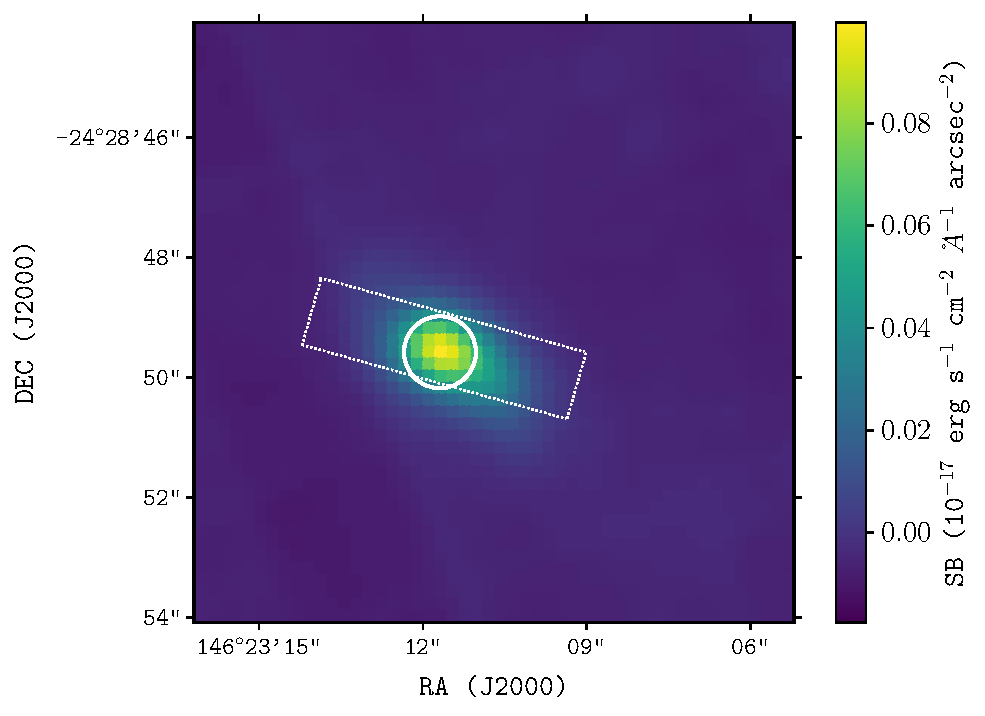
\includegraphics[width=0.7\columnwidth]{plots_chp3/0943-242_continuum_img.pdf}
\caption[MUSE line and continuum (white-light) image of MRC 0943-242]{MUSE line and continuum (white-light) image of MRC 0943-242. At the centre of the image is the high surface brightness region of the galaxy halo. The sub-cube aperture from which the spectrum in Fig. \ref{fig:0943-spectrum} is obtained is shown within the circle. The UVES slit (dotted outline) has a 1.2\arcsec width and extends over 5\arcsec.}
\label{fig:0943-continuum}
\end{figure}

\begin{sidewaysfigure*} 
\centering
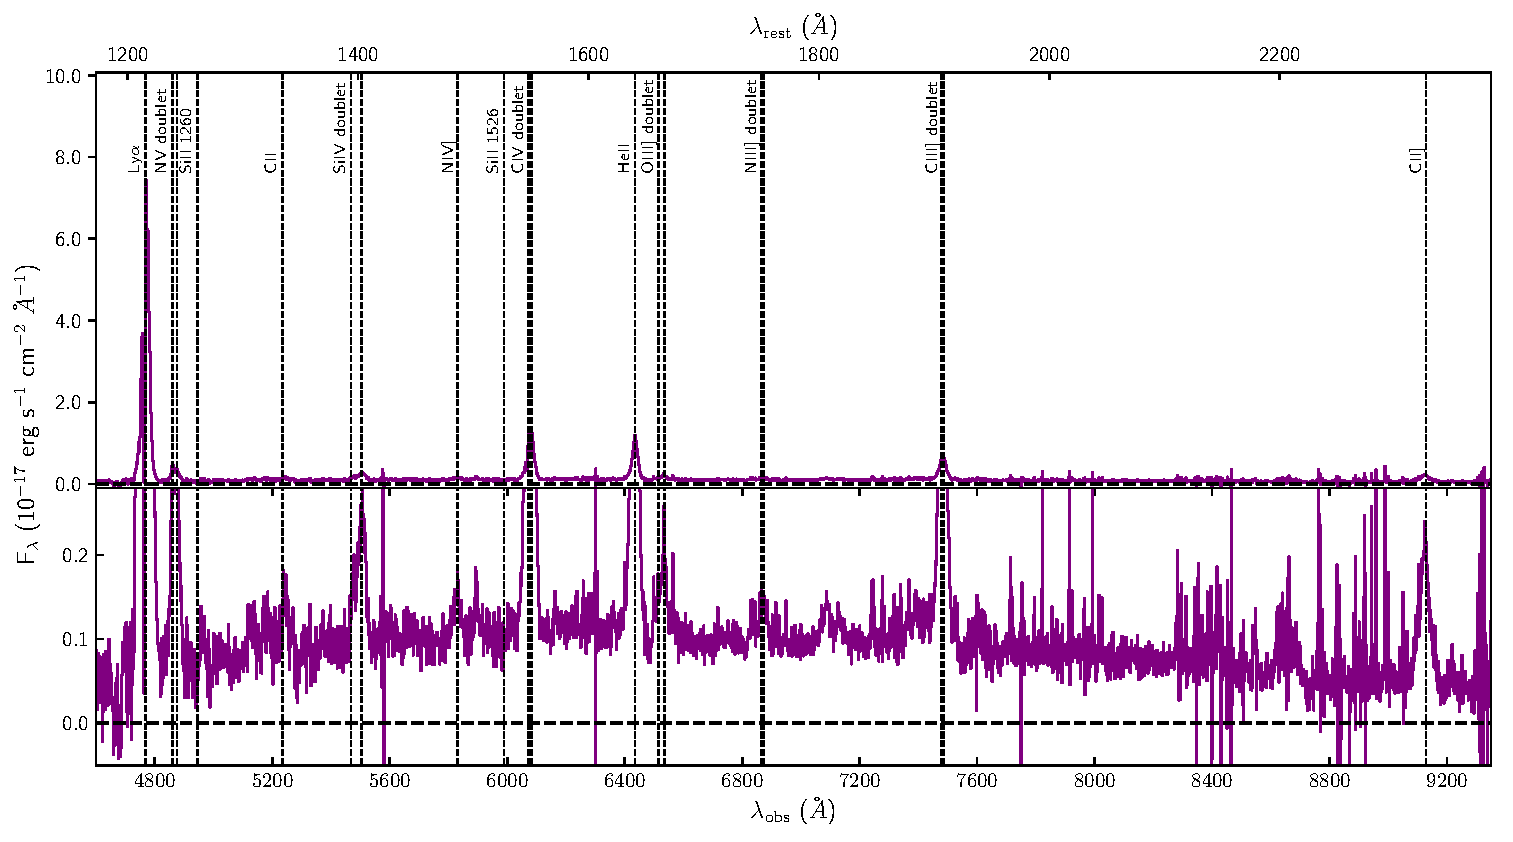
\includegraphics[width=\textwidth]{plots_chp3/0943-242_spectrum_3_pix_zoom.pdf}
\caption[MUSE spectrum of the bright nucleus in MRC 0943-243]{MUSE spectrum of the high surface brightness region in the halo of MRC 0943-243. The spectrum contains several rest-UV lines that are labelled and indicated by the dashed vertical lines. The upper panel shows the entire flux density range for the spectrum, while the lower panel covers only the low flux density range to show the lower S/N lines more clearly.}
\label{fig:0943-spectrum}
\end{sidewaysfigure*}

\subsection{Line-fitting procedure}
The goal of this work is to parametrise the physical conditions of gas in the halo of the radio galaxy Yggdrasil. To do this, we used the line profiles of ions that undergo resonant transitions, that is, \lya~$\lam$1216, \ion{C}{IV} $\lam\lam1548,1551$, \ion{N}{V} $\lam\lam1238,1243,$ and \ion{Si}{IV} $\lam\lam1393, 1402 $ (see Fig. \ref{fig:0943-spectrum}). We applied line-fitting procedures that combine Gaussian and Voigt models in order to characterise the emission and absorption simultaneously. The emergent emission is $F_\lam = F_{\lam,0} e^{-(\tau_{\lam,1} + ... + \tau_{\lam,n}) }$ for $n$ absorbers, where the unabsorbed emission, $F_{\lam,0},$ is denoted by the Gaussian function
\begin{equation}
F_{\lam,0} = \frac{ F }{ \sigma_\lam \sqrt{2\pi}} \exp\left[{-\frac{1}{2}\left(\frac{\lam - \lam_0}{\sigma_\lam}\right)^2}\right]
,\end{equation}
where $F$ is the integrated flux of the underlying emission, $\lam_0$ is the Gaussian line centre, $\sigma_\lam$ is the line width, and $\lambda$ is the wavelength.
The absorption is quantified by the optical depth, $\tau_\lam,$ which is denoted by the Voigt-Hjerting function
\begin{equation}
\tau_\lam = \frac{ N\sqrt{\pi} e^2 f \lam_0^2 }{ \Delta\lam_D m_e c^2 }H(a,u),
\end{equation}
where $N$ is the column density, $e$ (electron charge), $m_e$ (electron mass), and $c$ (light speed) are fundamental constants, and $f$ is the oscillator strength. $H(a,u)$ is the Hjerting function in which $a \equiv\frac{\Gamma\lam_0^2}{4\pi c \Delta\lam_D}$ and $u \equiv\frac{(\lam - \lam_0)}{\Delta\lam_D}$ such that $\Gamma$ is the Lorentzian width, $\Delta\lam_D$ is the Doppler parameter (also $b$ parameter), and $\lam - \lam_0,$ is the frequency shift from the line centre ($\lam_0$). $H(a,u)$ is obtained from the \citet{tepper-garcia2006} approximation, which is well suited for absorption systems that have column densities $ N/{\rm cm}^{-2} \leq10^{22}.$ When fitting the absorption, we also made the simplifying assumption that each cloud of absorbing gas covers the emission line region with a unity covering factor (C $\simeq$ 1.0).

We used the \pkg{python} package \pkg{lmfit} to carry out the non-linear least-squares fitting \citep{newville2016}. Our fitting method of choice was the Levenberg-Marquardt algorithm, which performs the $\chi^2$-minimisation that yields our best-fit results. In the figures, we report the reduced $\chi^2$-squared value, $\chi_\nu^2 = \chi^2/(N-N_i),$ where $N$ is the number of data points and $N_i$ is the number of free parameters. For each line, we calculated the local continuum level by masking the line emission and fitting a first-order polynomial to the surrounding continuum. The first-order polynomial was subtracted from both the line and continuum of \ion{He}{II} and Ly$\alpha,$ which are bright enough that not fitting the continuum has little effect on the overall fit. For \ion{C}{IV}, \ion{N}{V,} and \ion{Si}{IV}, which are lower in surface brightness (than \lya~and \ion{He}{II}), the continuum is likely to impact the overall fit.

Fitting Gaussian and Voigt functions simultaneously means that the composite model has many fit parameters. To prevent over-fitting and also to obtain a physical result, we used \lya~and \ion{He}{II} as initial guesses when we fitted underlying emission and absorption profiles to the \ion{C}{IV}, \ion{N}{V,} and \ion{Si}{IV}+\ion{O}{IV]} lines. 

From the \ion{He}{II} fit (described later in section \ref{section:Heii-fit}), we obtained the best-fit results for Gaussian fluxes (F$_\lam$), line widths ($\sigma_\lam$), and line centres ($\lam_0$). $\Delta\lam_{0,\ion{He}{II}}$ is the error on the fitted \ion{He}{II} line centre such that $\lam_{0,\ion{He}{II}} = 6436.09 \pm 0.30$ $\ang.$ The line centres are in agreement with the \ion{He}{II} systemic velocity (or zero velocity, which is fixed to the systemic redshift of the galaxy) within its uncertainties, that is, $\Delta\lam_{0,\ion{He}{II}} = 0.30$ $\ang$ = 10.3 km s$^{-1},$ under the assumption that all the emission originates from the centre of the halo. The \ion{He}{II} fit results for line width and the redshift of the line centre were set as initial guesses in Gaussian fits for emission in the resonant lines, \ion{C}{IV}, \ion{N}{V}, \ion{Si}{IV} and the non-resonant \ion{O}{IV],} which emits as part of the \ion{Si}{IV}+\ion{O}{IV]} intercombination line. Furthermore, we ensured that $F_\lam$ and $\sigma_\lam$ remain positive. 

To fit the \lya~absorption in the MUSE spectrum, we used the best-fit parameters from the literature \citep[i.e.][]{jarvis2003,wilman2004} as initial guesses in the fitting procedure. The best-fit \lya~absorber redshifts were passed on as initial guesses for absorber redshifts in the \ion{C}{IV}, \ion{N}{V,} and \ion{Si}{IV} line profiles. The initial guesses for column densities and Doppler parameters are based on rough estimates from the literature (i.e. \citealp{jarvis2003,wilman2004}, G16; S18). All three Voigt parameters have a limited parameter space over which a solution can be obtained. These parameter constraints are summarised in Table \ref{table:absorption-limits}. 

% redshift
In the fitting routine, some absorber redshifts were given more freedom to vary over a given parameter space than others because 
the ionisation energies of the different gas tracers, \ion{H}{I}, \ion{C}{IV}, \ion{N}{V,} and \ion{Si}{IV}, differ greatly such that E$_\ion{H}{I}$ = 13.6 eV, E$_\ion{C}{IV}$ = 64.5 eV, E$_\ion{N}{V}$ = 97.9 eV, and E$_\ion{Si}{IV}$ = 45.1 eV. It would be unrealistic to expect them to exist at exactly the same redshifts. 

% Doppler parameter
The minimum Doppler parameter permissible in the line-fitting is set by the lower limit of the MUSE spectral resolution, which suggests that an approximate lower limit of $b_{\rm min} \sim \sigma_\lam = 90$ km s$^{-1}$ / 2.3548 $\simeq$ 40 km s$^{-1}.$ We set a conservative upper limit of $b_{\rm max} = 400$ km s$^{-1}$ for \ion{C}{IV}, \ion{N}{V,} and \ion{Si}{IV} with the understanding that the absorbing gas is kinematically quiet in relation to perturbed gas regions that have FWHM $\geq$ 1000 km s$^{-1}.$ 

% column density
In general, \lya~absorbers in HzRG gas nebulae are found to have low column densities of $N_\ion{H}{I}/{\rm cm}^{-2} = 10^{13} - 10^{15}$ or be optically thick with column densities of $N_\ion{H}{I}/{\rm cm}^{-2} > 10^{18}$  \citep{wilman2004}. Because \ion{H}{I} is frequently more abundant than metals in halo gas environments, we can expect the column densities of the metal ions to be lower. Hence, we set the lower and upper limits for permissible fitted column densities to $N/{\rm cm}^{-2} = 10^{12} - 10^{20}$ cm$^{-2}.$ A full summary of the initial boundary conditions in the fitting procedure is given in Table \ref{table:absorption-limits}. The physical constraints placed on the line-fitting procedure by quantum rules are highlighted in Table \ref{table:absorption-rules}. 

\section{Best-fit line models}\label{section:best-fit-line}
\subsection{\ion{He}{II}}\label{section:Heii-fit}
\ion{He}{II} $\lam$1640 is the brightest non-resonant emission line and forms the basis of our estimation of the underlying emission profiles of the lines we study here, that is, Ly$\alpha,$ \ion{C}{IV}, \ion{N}{V,} and \ion{Si}{IV}. In the extracted spectrum, we obtained a detection of \ion{He}{II} emission that forms through cascade recombination of He$^{++},$ which emits a non-resonant photon. The \ion{He}{II} lines are often used to determine the systemic redshift of a galaxy (e.g. \citealp{reuland2007,swinbank2015}; S18). Although \lya~is brighter than \ion{He}{II}, we refrained from using \lya~for this purpose because of its susceptibility to radiative transfer effects that clearly affect the emergent line emission.

The \ion{He}{II} line, shown in Fig. \ref{fig:HeII-line}, has an excess of emission at $\Delta \varv \sim-1000$ km s$^{-1}$ that is not present at $\Delta \varv \sim1000$ km s$^{-1}$ , indicating asymmetry. This has been identified before in \citet{jarvis2003}, where the excess was found to have little effect on the final fit. Our 1D spectrum has brighter line detections, and to account for the excess emission in the wing, we therefore fit the \ion{He}{II} line with two Gaussian profiles: one for emission blueshifted relative to, and another for emission originating from, the systemic velocity. This method has been employed frequently for fitting asymmetric line profiles from various gas phases \citep[e.g.][]{mullaney2013,cicone2014,rakshit2018,hernandez-garcia2018,perna2019}. 

\begin{figure} 
\centering
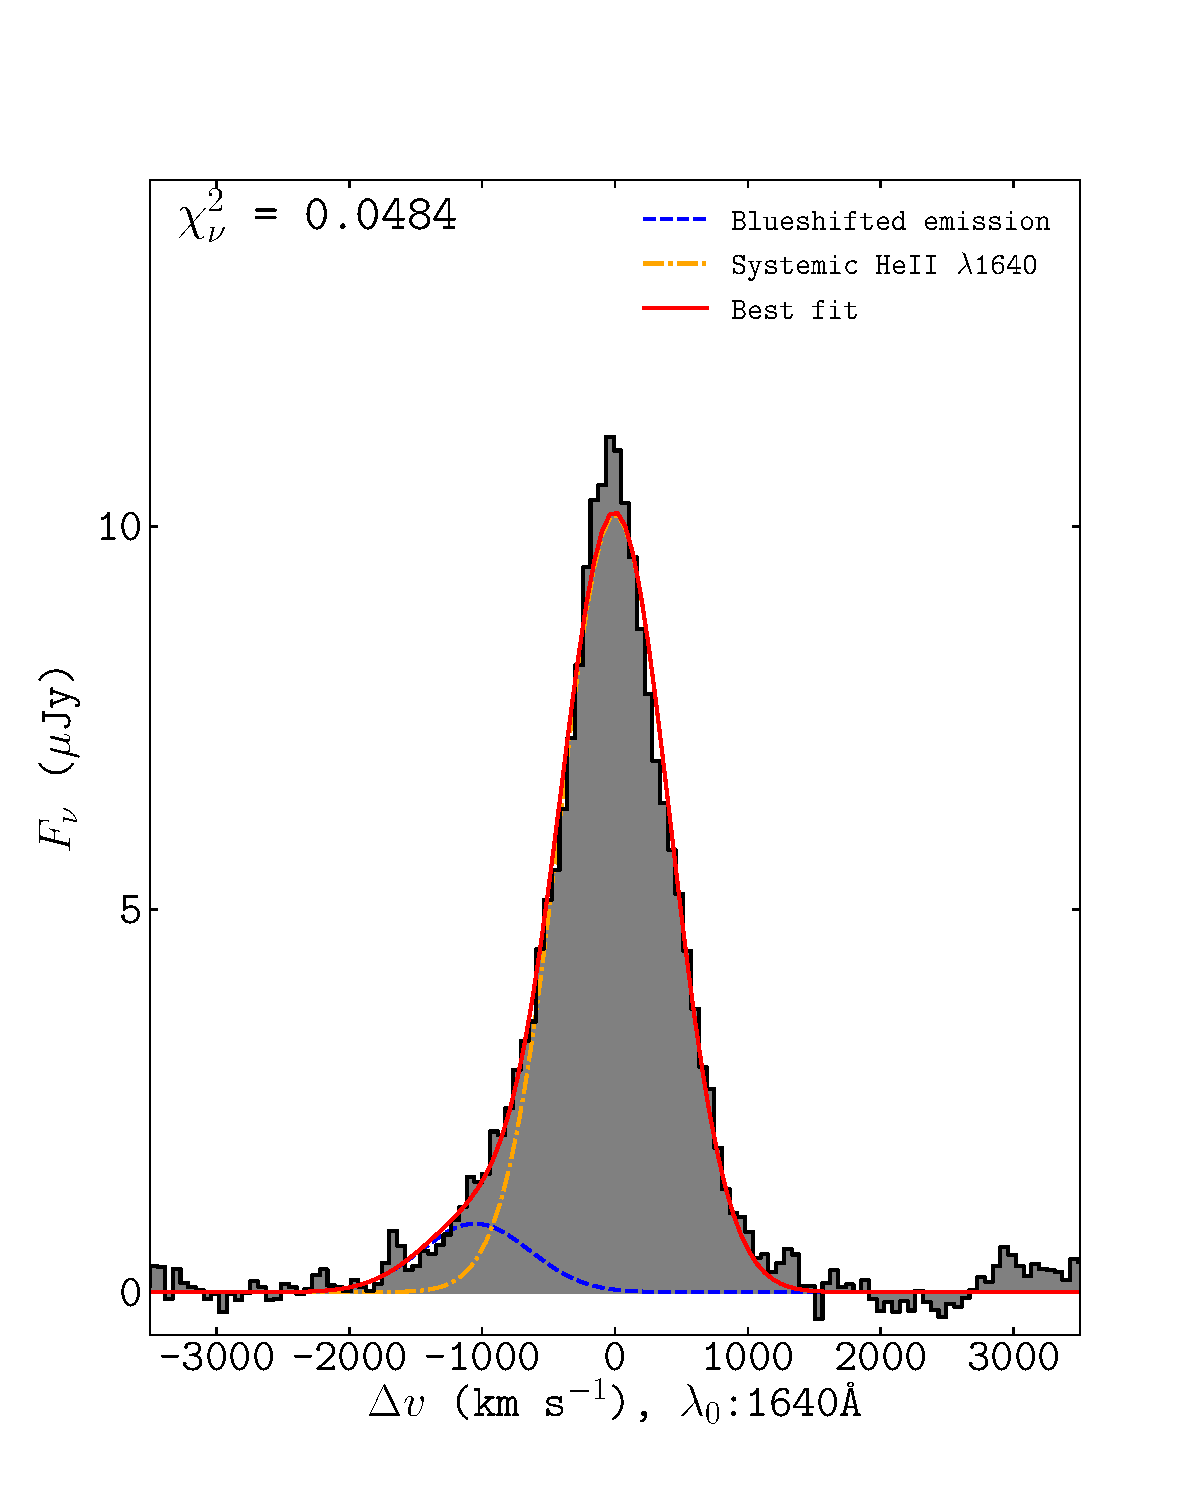
\includegraphics[width=0.6\columnwidth]{plots_chp3/HeII_fit.pdf}
\caption[\ion{He}{II} $\lam$1640 line in MUSE and its best-fit]{\ion{He}{II} $\lam$1640 line in the MUSE spectrum (shown in Fig. \ref{fig:0943-spectrum}). The line profile has been continuum subtracted. The best-fit model (red) consists of two Gaussian profiles. The first Gaussian component (in blue) models the excess blue wing emission at the negative velocities, while the second component (in orange) models the emission at the systemic velocity of the galaxy. }
\label{fig:HeII-line}
\end{figure}

We estimated the central velocity of the excess emission in \ion{He}{II} by spatially identifying where its emission peaks in surface brightness (explained further in section \ref{method:blueshifted-emission}). The best-fit Gaussian parameters obtained from the spatially offset region were used to fit the blueshifted emission as a second component to the emission from the HSBR at the systemic velocity. The result of this fitting procedure is shown in Fig. \ref{fig:HeII-line}, where the additional component is broadened to a line width of FWHM $\simeq1000$ km s$^{-1}$ and also blueshifted from the systemic velocity. From the \ion{He}{II} best-fit result, we obtain a fiducial systemic redshift of z$_{\rm sys}$ = $2.9235 \pm 0.0001$ that denotes the zero velocity for all the lines identified in Fig. \ref{fig:0943-spectrum}.

\subsection{\ion{H}{I} \lya}\label{section:Lya-fit}

\ion{H}{I} \lya~$\lam$1216 is the brightest line in the rest-UV spectrum. We fit the \lya~emission envelope with a double Gaussian: one to the non-absorbed singlet emission at the line centre, and another to the strong blue wing emission at $\Delta \varv \simeq -1000$ km s$^{-1}$ (see Fig. \ref{fig:Lya-line-muse-uves}). The motivation for including a second emission component to the \lya~fit is twofold: a) it is well detected in the emission line \ion{He}{II} and therefore likely to also emit in \lya, and b) there is an asymmetry between emission at the blue and red wings of Ly$\alpha.$ Once fit, we see that including a second Gaussian improved the \lya~emission fit. 

The updated Gaussian fit describes the \lya~profile well in both MUSE and UVES spectra and the best-fit parameters are in good agreement with the literature (see Tables \ref{table:absorption-fits-uves} and \ref{table:emission-fits-uves}). This is expected because \lya~is affected by radiative transfer effects and is therefore less likely to have a symmetric emission profile. There is also an additional underlying kinematic component causing the blue wing excess, based on the \ion{He}{II} line fit (see Fig. \ref{fig:HeII-line}). 

To account for the absorbers, we fit four Voigt profiles, as has been done in previous works on this topic (i.e. \citealp{vanojik1997,jarvis2003,wilman2004}; G16; B18). We also convolved the Voigt profiles with the line-spread function (LSF) of MUSE, using a fast-Fourier transform similar to that used to convolve Voigt and LSF profiles in the package, \pkg{vpfit} \citep{krogager2018}. The LSF or instrumental profile (IP) of MUSE, when convolved with the Voigt profile, has an average Gaussian width of $<\sigma_\lam>$ = 2.65 $\ang.$ 

We show the line-fitting result for \lya~in Fig. \ref{fig:Lya-line-muse-uves}a. Below this, in Fig. \ref{fig:Lya-line-muse-uves}b, we show a similar fit to the \lya~profile as was detected with UVES, which has an LSF with an average Gaussian width of $<\sigma_\lam>$ = 0.3 $\ang.$ 

\begin{figure} 
\centering
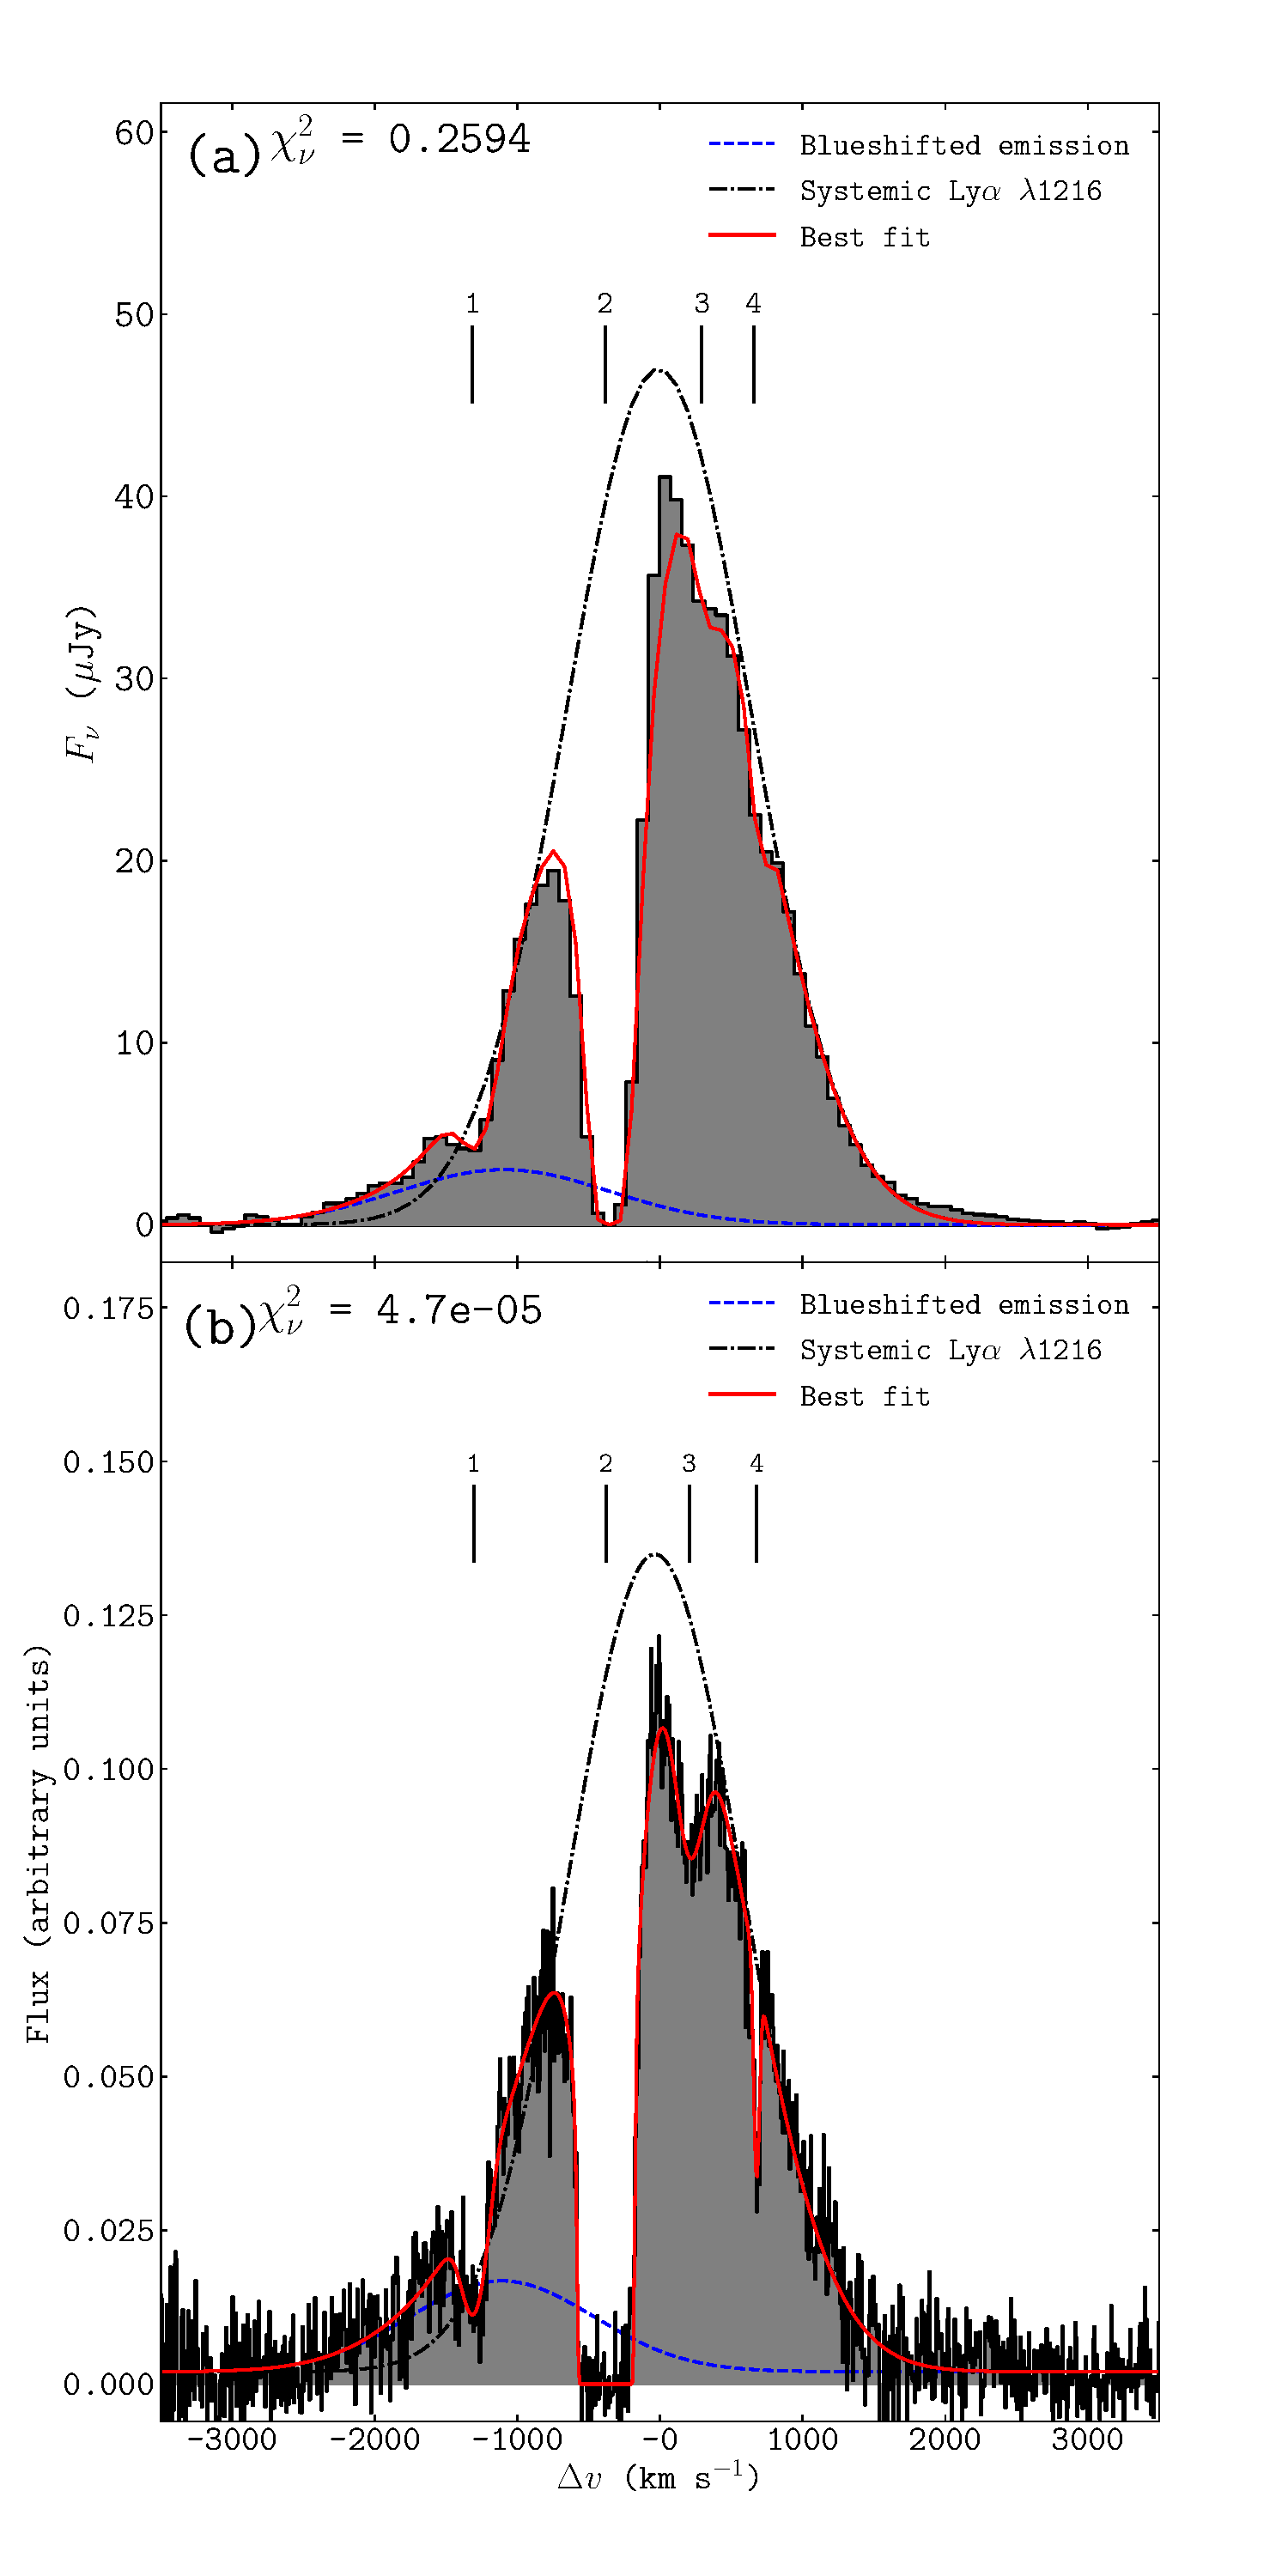
\includegraphics[width=0.6\columnwidth]{plots_chp3/Lya_fit_uves_muse_blue_fit.pdf}
\caption[\lya~$\lam1216$ line in MUSE and its best-fit]{MUSE-detected continuum-subtracted \lya~($upper$) and ancillary UVES-detected \lya~($lower$) for Yggdrasil. The best-fit line model (red) combines \lya~emission consisting of blueshifted and systemic components, as well as the four known absorption troughs.}
\label{fig:Lya-line-muse-uves}
\end{figure}

The \lya~absorber redshifts are used to predict the most probable redshifts for the absorbers, in general. In particular, the redshifts of the absorbers associated with resonant metal ions, \ion{C}{IV}, \ion{N}{V,} and \ion{Si}{IV}, are constrained to stay within $4\Delta{\rm z_{sys}}$  (where $\Delta{\rm z_{sys}} =1.35\e{-4}$) agreement of the measured \lya~absorber redshifts. This is done following the hypothesis that \lya~absorption occurs within roughly the same volume of gas as absorption of photons associated with the resonant transitions. 

For this to occur, there would need to be a very strong ionising continuum to produce all of the observed ions, which is possible with ionisation by the AGN. The different ionisation energies also imply that fixing the absorbers to exactly the same redshift is unrealistic. This is why we allowed the fitted absorber redshifts to vary over a parameter space that depends on how tightly a parameter needed to be constrained. 

\subsection{\ion{C}{IV} and \ion{N}{V}}\label{section:CIV-NV-fit}

We have obtained detections of \ion{C}{IV} $\lam\lam1548,1551$ and \ion{N}{V} $\lam\lam1238,1243$. Given that \lya~absorber 4 is narrow, it is likely to suffer the highest degree of instrumental broadening in MUSE, as seen in Fig. \ref{fig:Lya-line-muse-uves}b. For \ion{C}{IV} and \ion{N}{V}, we therefore did not include a fourth absorber in the model. At the MUSE spectral resolution we expect to lose any absorption signal from such a narrow absorber. The Voigt profiles were, as with Ly$\alpha,$  convolved with the LSF of MUSE. 

The observed emission in the doublet lines, \ion{C}{IV} and \ion{N}{V}, was fit with two Gaussian functions that were constrained according to atomic physics (all constraints are summarised in Table \ref{table:absorption-rules}). The local continuum was estimated using a  separate linear polynomial fit (to the continuum only, with line emission masked). The continuum was thus fixed during fitting. Additionally, in \ion{C}{IV}, we fit a second component to each of the doublet lines to account for the blueshifted emission seen in \ion{He}{II,} which has a similar S/N level as \ion{C}{IV}. \ion{N}{V} has a lower S/N than both of these lines, therefore the blueshifted emission is likely to be negligible in this fit. 

We obtained atomic constants such as rest wavelengths and oscillator strengths from the database provided by \citet{cashman2017}. For doublet lines, the ratios of line centres (i.e. $\lam_1/\lam_2$) and rest-frame wavelengths were fixed to one another. The doublet emission originates from the same gas, therefore the doublet line widths are equal, that is, $\sigma_{\lam,1} = \sigma_{\lam,2}$. The doublet ratios (DR = $F_1/F_2$) were fixed to the those of the oscillator strengths such that they are DR = 2. Doublet ratios of 2 are observed frequently in quasar absorption lines. This is particularly true for \ion{C}{IV} lines, whose doublet ratios vary from 2 to 1 from the linear to the saturated absorption regimes \citep{peroux2004}. Assuming that \ion{C}{IV} and \ion{N}{V} absorbers 1 and 3 are not saturated and have a unity covering factor, C $\simeq$ 1.0, because their emission does not reach zero flux level at the absorber velocities, we set DR = 2 when fitting.

The best-fit models for \ion{C}{IV} and \ion{N}{V} are shown in Figs~\ref{fig:CIV-and-NV-lines}a and \ref{fig:CIV-and-NV-lines}b. The emission and absorption fit results are shown in Tables \ref{table:absorption-fits} and \ref{table:emission-fits}, respectively. We note that both \ion{C}{IV} and \ion{N}{V} fits feature a slight kink at $\Delta \varv$ $\sim -2000$ km s$^{-1}.$ This may be the result of the column density of absorber 1 being over-estimated at this velocity, which could imply that the blueshifted \ion{C}{IV} emission is not impeded by absorber 1, as we have assumed. Rather, absorber 1 covers the emission line region behind it, the blueshifted emission. Determining which absorbers cover the systemic and/or the blueshifted emission is a task that will require higher spatial and/or spectral resolution. For simplicity, we assumed that all three absorbers impede the systemic, blueshifted, and continuum emission components.


\begin{figure}
        \subfloat[\ion{C}{IV} doublet line]{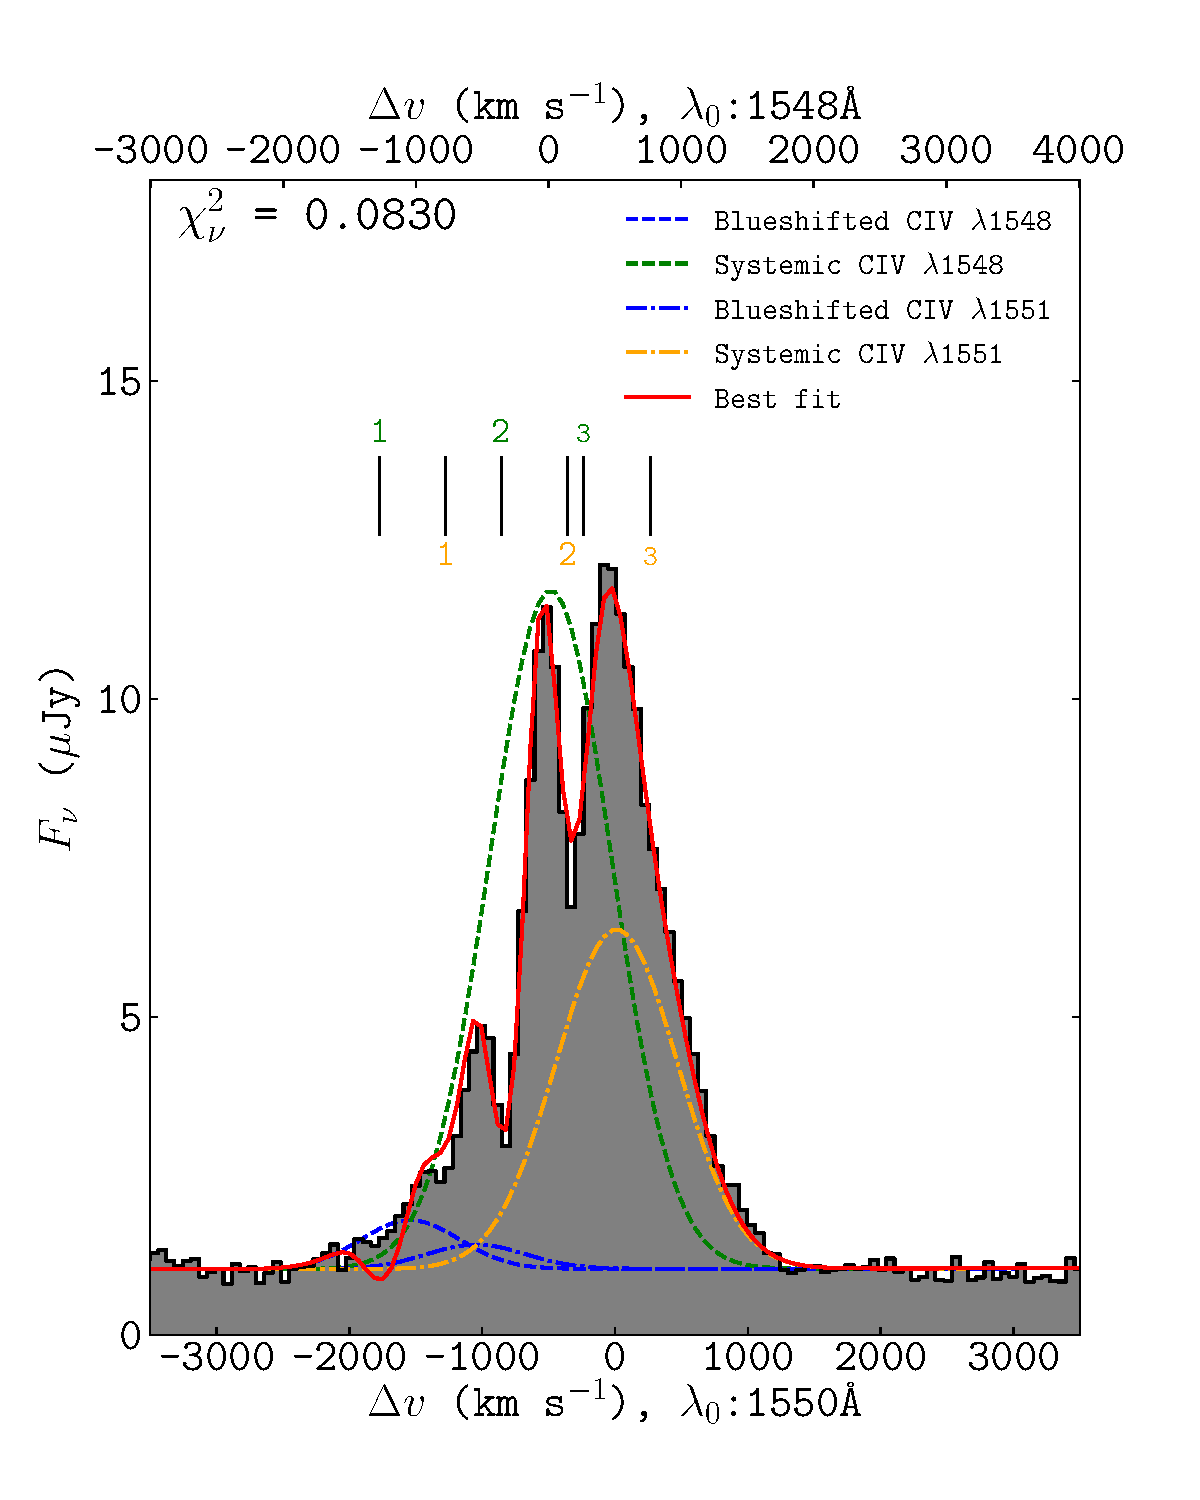
\includegraphics[width=0.52\columnwidth]{plots_chp3/CIV_fit.pdf}}
        \subfloat[\ion{N}{V} doublet line]{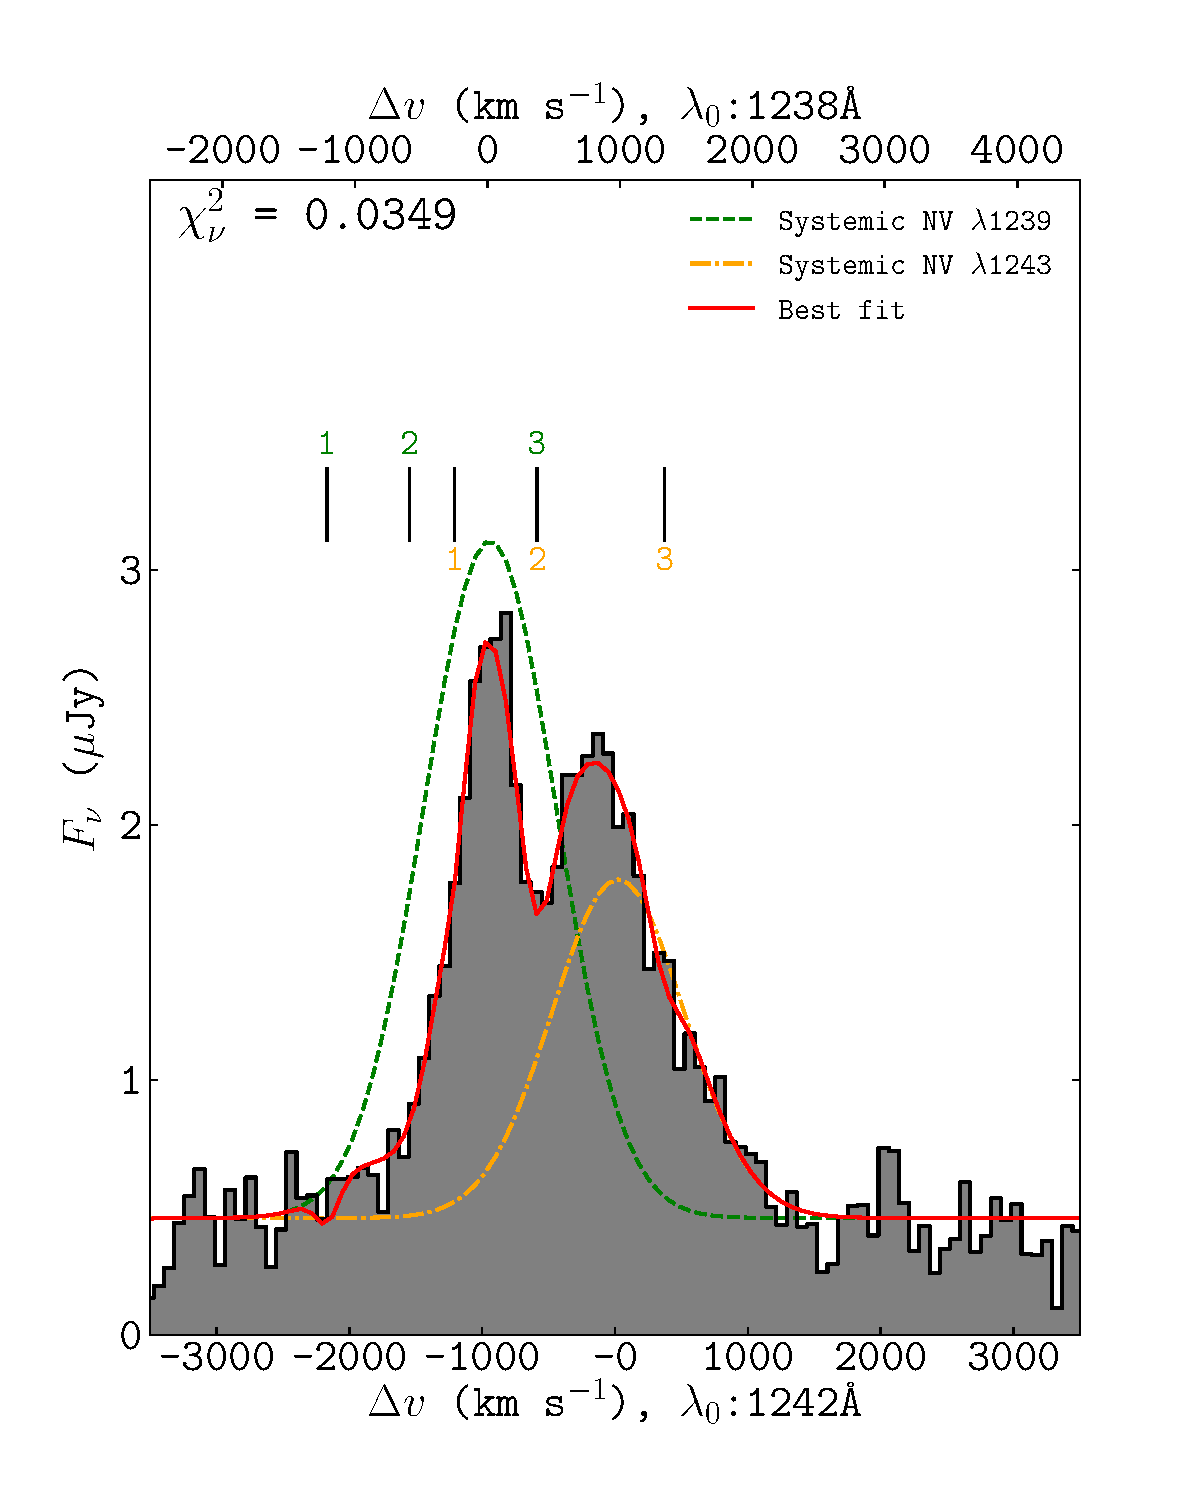
\includegraphics[width=0.52\columnwidth]{plots_chp3/NV_fit.pdf}}\\
\caption[\ion{C}{IV} $\lam\lam1548,1551$ and \ion{N}{V} $\lam\lam1238,1243$ lines in MUSE and their best-fits]{Panel (a): Best-fit line model fit to \ion{C}{IV} $\lam\lam1548,1551$ detected with MUSE. The green and orange dashed lines represent the underlying doublet emission at wavelengths of 1548 $\ang$ and 1551 $\ang,$ which are the rest-frame velocities, in the $\text{upper}$ and $\text{lower}$ axes, respectively. Three Voigt profiles model the absorbers for each emission line in the doublet. Panel (b): Best-fit line model for \ion{N}{V} $\lam\lam1238,1243$ detected with MUSE. The green and orange dashed lines represent the underlying doublet emission at wavelengths of 1548 $\ang$ and 1551 $\ang,$ which are the rest-frame velocities, in the $\text{upper}$ and $\text{lower}$ axes, respectively. Three Voigt profiles model the absorbers for each emission line in the doublet. }
\label{fig:CIV-and-NV-lines}
\end{figure}

% \begin{figure} 
% \centering
% 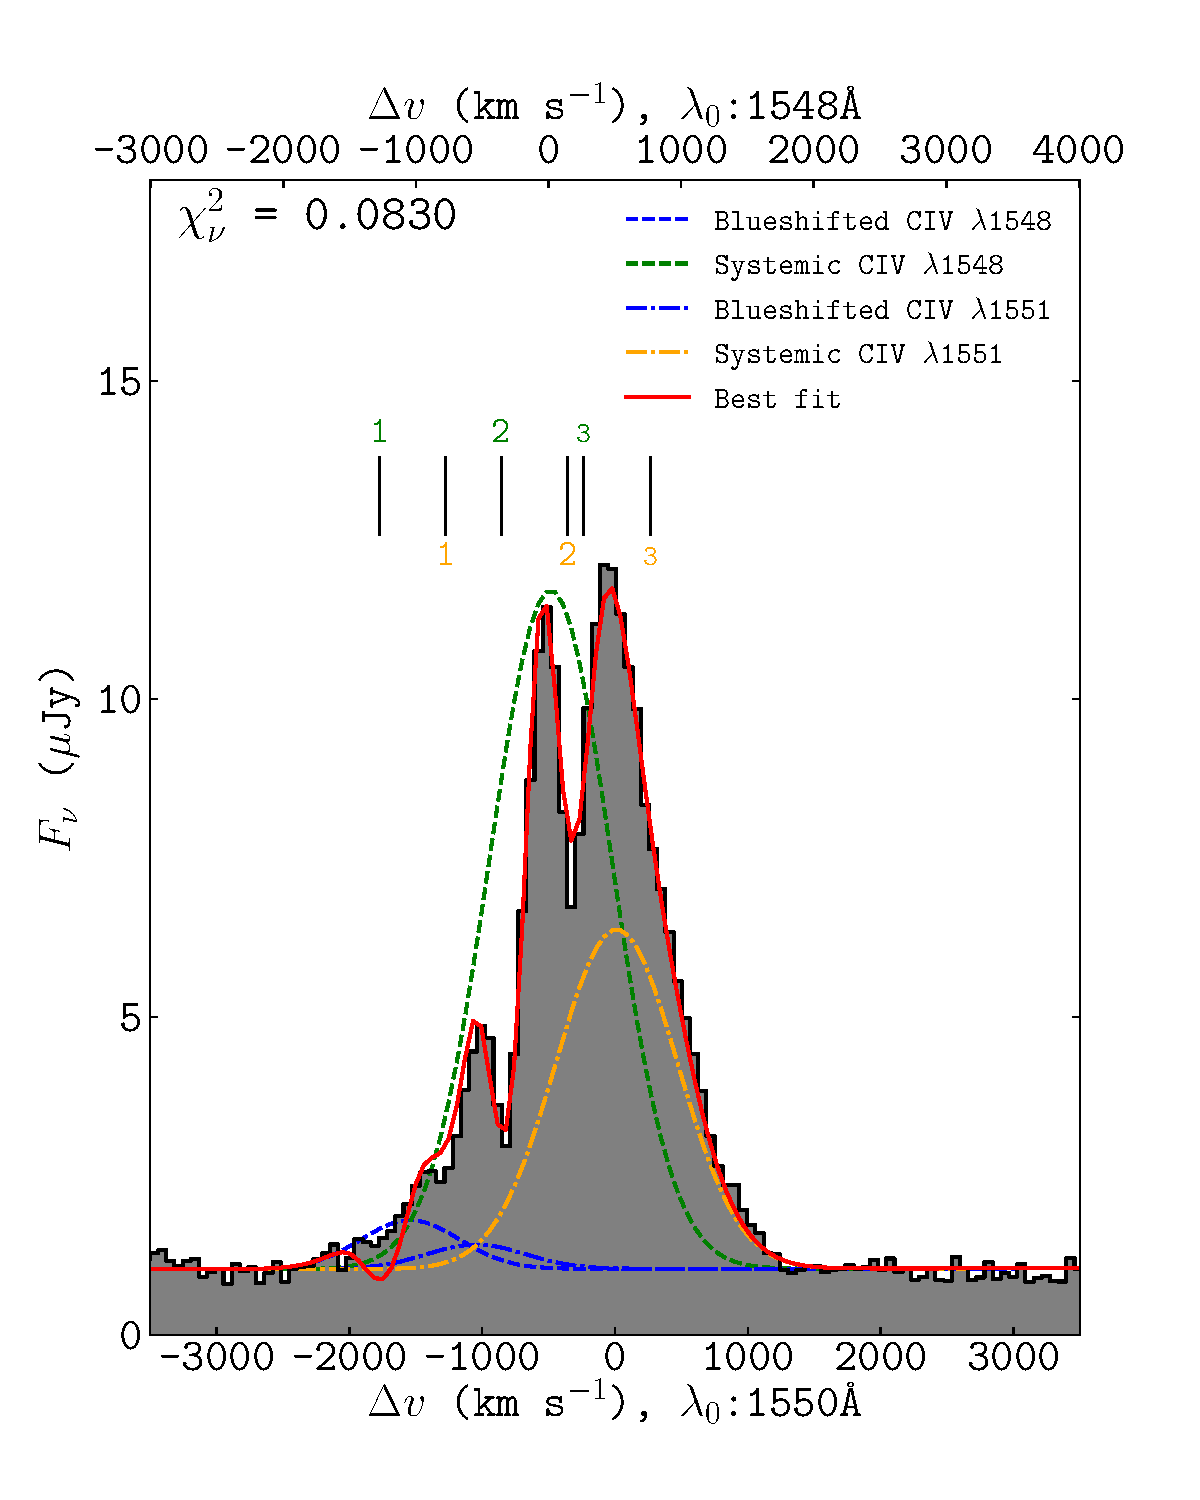
\includegraphics[width=0.6\columnwidth]{plots_chp3/CIV_fit.pdf}
% \caption{Best-fit line model fit to \ion{C}{IV} $\lam\lam1548,1551$ detected with MUSE. The green and orange dashed lines represent the underlying doublet emission at wavelengths of 1548 $\ang$ and 1551 $\ang,$ which are the rest-frame velocities, in the $\text{upper}$ and $\text{lower}$ axes, respectively. Three Voigt profiles model the absorbers for each emission line in the doublet.}
% \label{fig:CIV-line}
% \end{figure}

% \begin{figure} 
% \centering
% {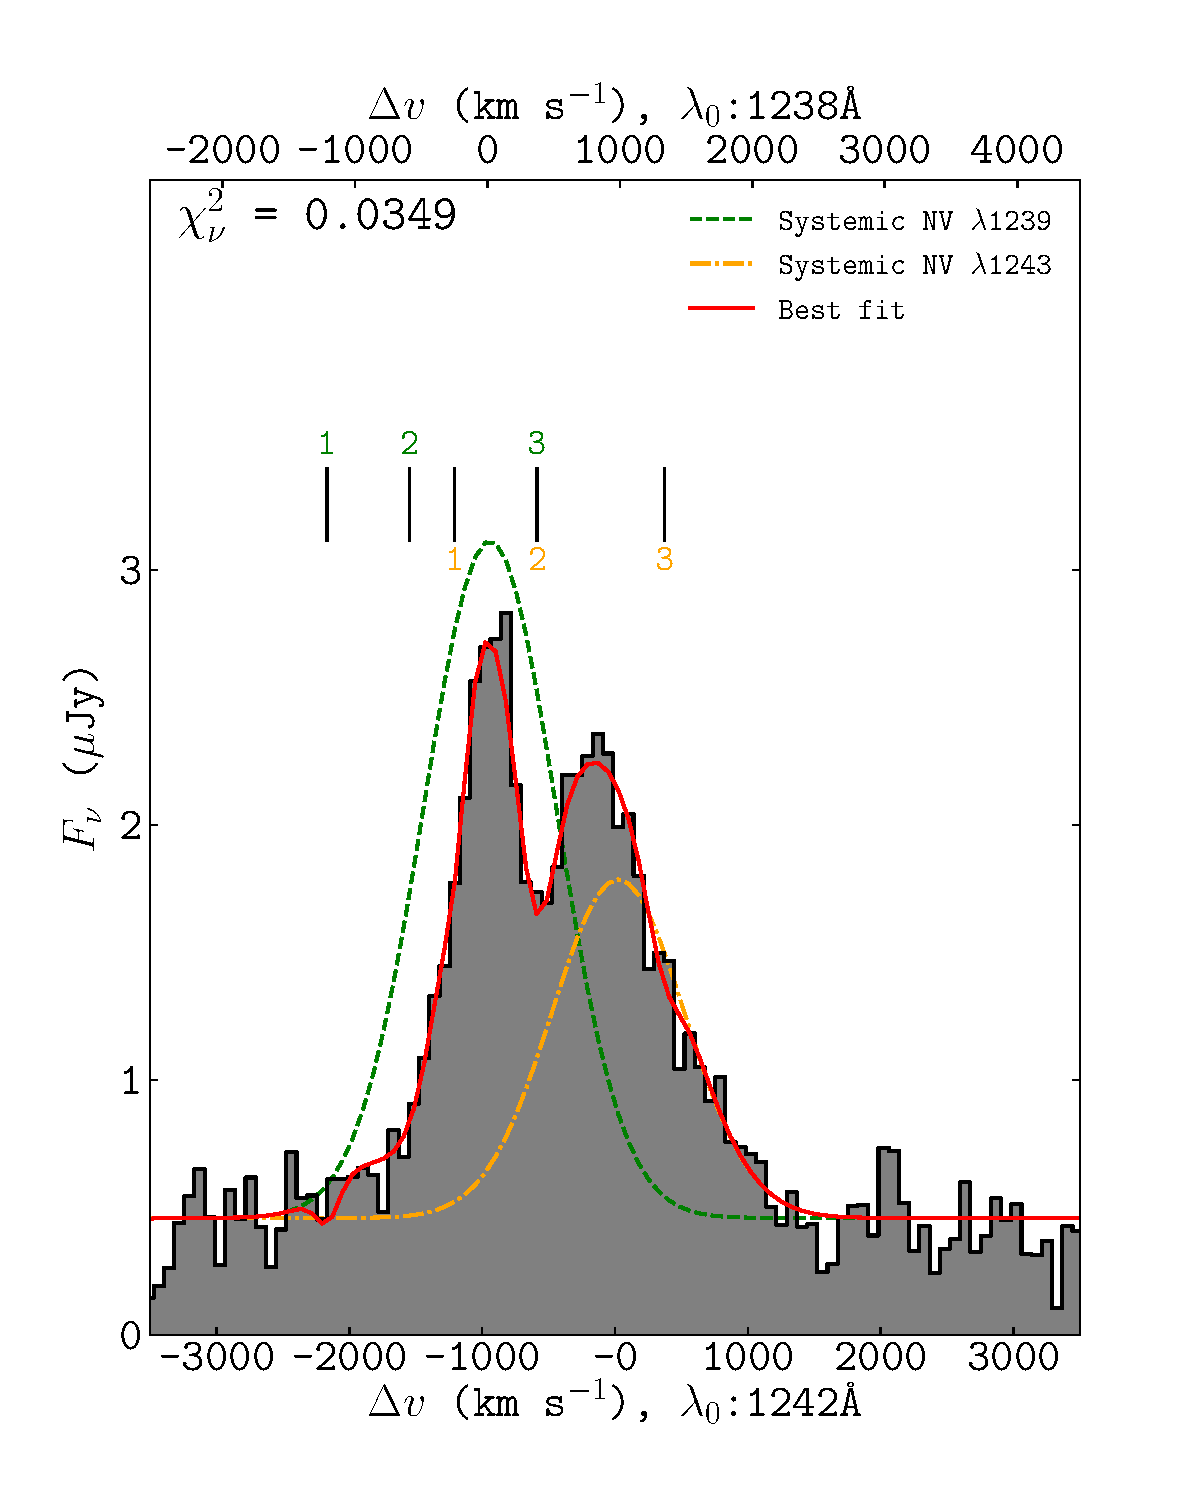
\includegraphics[width=0.6\columnwidth]{plots_chp3/NV_fit.pdf}}
% \caption{Best-fit line model to \ion{N}{V} $\lam\lam1238,1242$ detected with MUSE. The green and orange dashed lines represent the underlying doublet emission at the rest-frame wavelengths 1238 $\ang$ and 1242 $\ang,$ which are fixed to the systemic velocity in the $\text{upper}$ and $\text{lower}$ axes, respectively. Three Voigt profiles model the absorbers for each emission line in the doublet. }
% \label{fig:NV-line}
% \end{figure}

\begin{figure} 
\centering
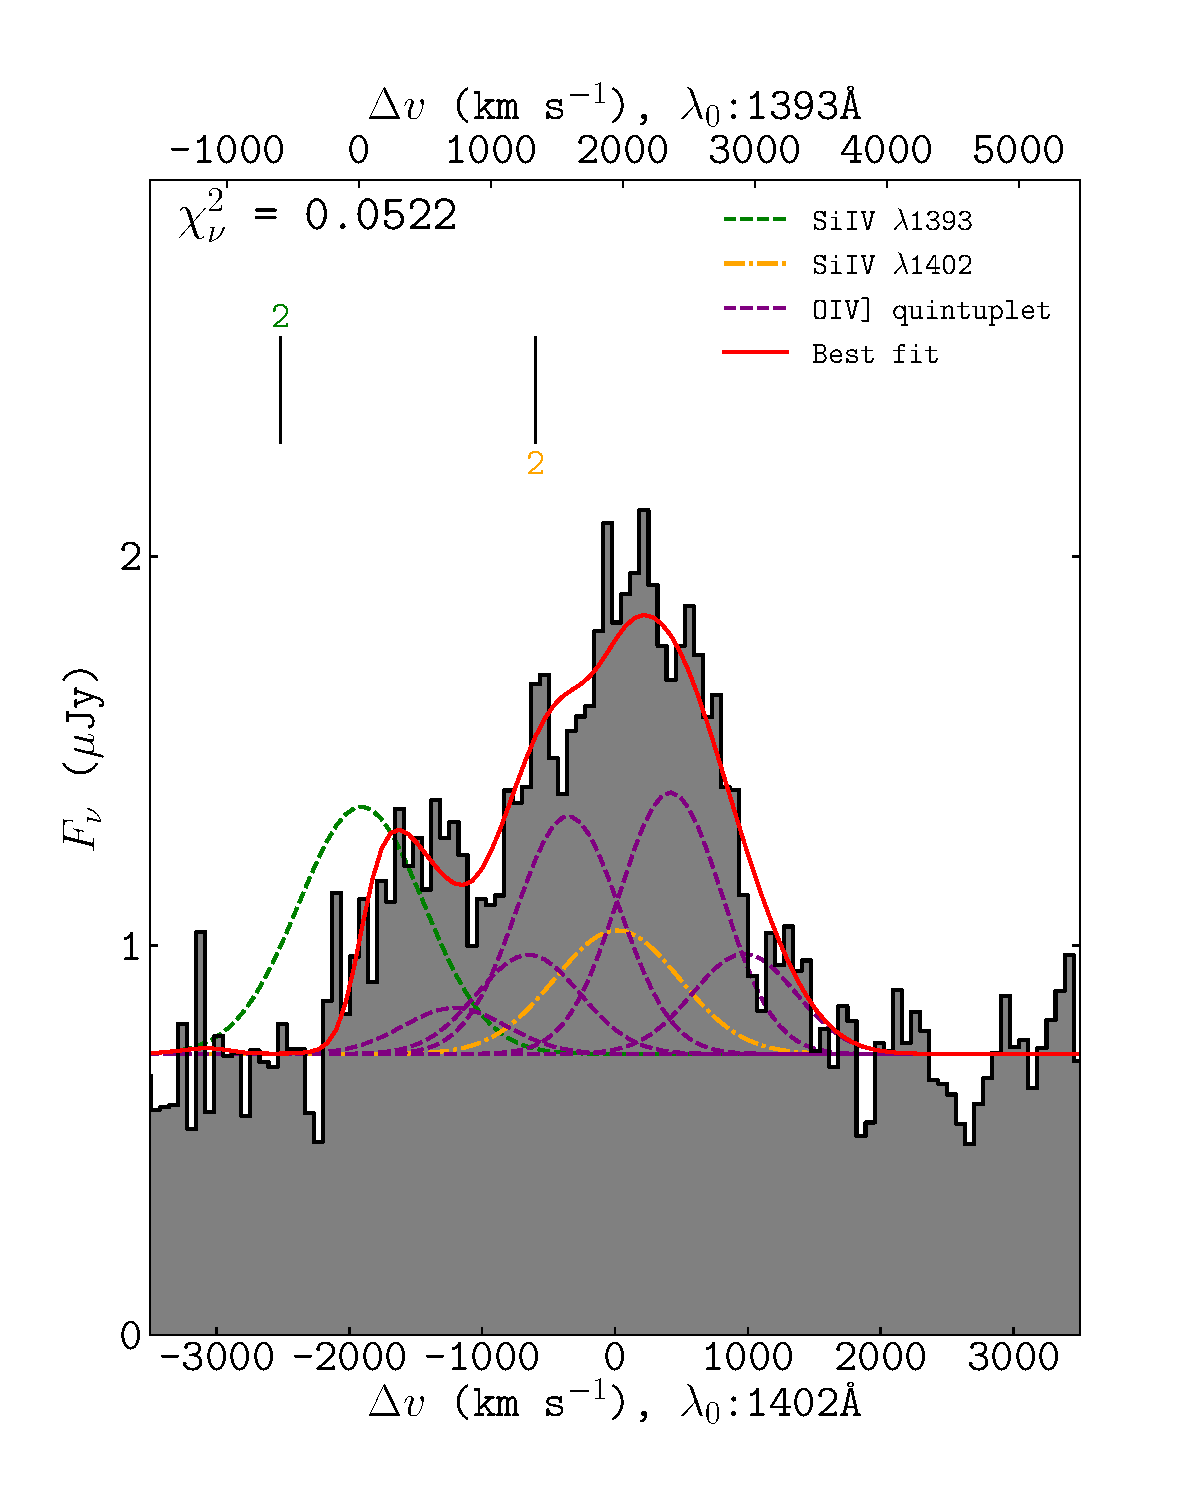
\includegraphics[width=0.55\columnwidth]{plots_chp3/SiIV_fit.pdf}
\caption[\ion{Si}{IV} $\lam\lam1393,1402$ + \ion{O}{IV]} intercombination line in MUSE and its best-fit]{Best fit line model to the intercombination \ion{Si}{IV} $\lam\lam1393,1402$ + \ion{O}{IV]} line detected with MUSE. The green and orange dashed lines represent the underlying doublet emission at the rest-frame wavelengths, 1393 $\ang$ and 1402 $\ang,$ which are fixed to the systemic velocity in the upper and lower axes, respectively. The \ion{O}{IV]} quintuplet line emission is shown in purple.}
\label{fig:SiIV-line}
\end{figure}

\subsection{\ion{Si}{IV}+\ion{O}{IV}]}\label{section:SiIV-fit}

The detected \ion{Si}{IV} $\lam\lam1393,1402$ line doublet overlaps with emission from the \ion{O}{IV]} quintuplet. \ion{Si}{IV} is a resonant line, and we modelled it with an absorption line at the same velocity as \lya~absorber 2. We did not include absorbers 1 and 3 because the fit did not change significantly when they were added.  

As before, the Voigt profile was convolved with the LSF of MUSE and the \ion{Si}{IV} doublet emission  was modelled by two Gaussians. Again, we fixed the continuum to the result of the linear polynomial fit of the local continuum (while the line emission was masked). The \ion{O}{IV]} quintuplet comprises five emission components at the rest-frame wavelengths for \ion{O}{IV],} which are 1397.2 $\ang$, 1399.8 $\ang$, 1401.2 $\ang$, 1404.8 $\ang$, and 1407.4 $\ang.$ To fit these, we used five Gaussian profiles with equal line widths. The quintuplet ratios were set by the oscillator strengths of each transition. We show the fit for the intercombination \ion{Si}{IV}+\ion{O}{IV]} lines in Fig.~\ref{fig:SiIV-line}, and the absorption fit results are shown in Table \ref{table:absorption-fits} and those for emission in Table \ref{table:emission-fits}. 

In an attempt to confirm the consistency of this result, we compared the fluxes of the same \ion{Si}{IV} and \ion{O}{IV]} lines detected at high spectral resolution for the binary symbiotic star RR Telescopii, which is shown in Fig. 5 of \citet{keenan2002}. The best-fit flux ratios for \ion{O}{IV]} are consistent with those of the high-resolution stellar spectrum, which is the perhaps the best observational comparison available for \ion{Si}{IV} and \ion{O}{IV]} intercombination line fluxes. 

\begin{table*}
\caption[Boundary conditions from line-fitting routine]{Lower and upper bounds placed on initial conditions in the line-fitting routine.
\newline {\it Note:}$\Delta$ is the largest permissible deviation (from the initial guess) imposed on a fit parameter.}
\centering
\begin{tabular}{ l  l }
\hline \hline
Fit parameters & Boundary conditions \\
                                                                                                                & \\
  \hline
                                                                                                                & \\
\bf{Gaussian (for emission):}                   & \\
                                                                                                                & \\
Line centre, $\lam_0$ (\ang)                                    & $\Delta \lam_0 = 0.3$ \\
Line flux, $F$ (erg s$^{-1}$ cm$^{-2}$) & $F \geq$ 0 \\
Line width, $\sigma_\lam$ (\ang)                        & $\sigma_\lam > 0$ \\                                                           
                                                                                                                & \\
 \hline
                                                                                                                & \\
\bf{Voigt (for absorption):}                            & \\
                                                                                                                & \\
\underline{Redshift, $z$:}                              & \\    
 \lya                                                                                                   &       $\Delta z_1 \leq 5.0\e{-3}$  \\
                                                                                                                &       $\Delta z_2 \leq 1.0\e{-3}$ \\
                                                                                                                &       $\Delta z_3 \leq 4.0\e{-3}$ \\
                                                                                                                &       $\Delta z_4 \leq 3.0\e{-3}$ \\
\ion{C}{IV}                                                                             & $\Delta z_n \leq 6.0\e{-4}$\\
\ion{Si}{IV} and \ion{N}{V}                             & $\Delta z_n \leq 6.0\e{-3}$\\
                                                                                                                                                & \\
\underline{Doppler parameter, $b$ (km s$^{-1}$):}                       & \\                                                                                                                              
Ly$\alpha,$ \ion{C}{IV}, \ion{N}{V,} and \ion{Si}{IV}                    & 40 $\leq b \leq$  400 \\
                                                                                                                                                & \\
\underline{Column density, $N$ (cm$^{-2}$): }   & \\
\lya                                                                                                                                    & 10$^{12}$ $\leq N \leq$ 10$^{20}$ \\
\ion{C}{IV}, \ion{N}{V,} and \ion{Si}{IV}                                & 10$^{13}$ $\leq N \leq$ 10$^{16}$ \\                    
                                                                                                                                                & \\
  \hline
\end{tabular}
\label{table:absorption-limits}
\end{table*}

\begin{table*}
\caption[Line constraints imposed by atomic physics]{Line constraints, set by atomic physics, are embedded in the fitting to obtain best-fit results for \ion{C}{IV}, \ion{N}{V,} and \ion{Si}{IV}+\ion{O}{IV]}. The flux ratios (${F_1}/{F_2}$) are equal to the oscillator strength ratios ($f_1/f_2$). The line centre ratios ($\lam_{0,1}/\lam_{0,2}$) are equal to the rest-frame wavelength ratios ($\lam_1/\lam_2).$ The redshift, $z,$ Doppler parameter, and column density, $N,$ are equal between doublet wavelengths. The \ion{O}{IV]} quintuplet constraints are similar to those of the doublets. The fourth quintuplet line, 1404.8 $\ang,$ is the brightest of the \ion{O}{IV]} quintuplets, therefore the other four \ion{O}{IV]} lines are fixed to it. }
\centering
\begin{tabular}{ l  l }
\hline \hline
Fit Parameters &  Rules \\
        & \\
 \hline
        & \\
 \underline{Gaussian parameters for doublet lines:}     & \\
        & \\
Line centre, $\lam_0$ (\ang)                                                    & $\frac{\lam_{0,1}}{\lam_{0,2}} = \frac{\lam_1}{\lam_2}$ \\
Line flux, $F$ (erg s$^{-1}$ cm$^{-2}$)         & $\frac{F_1}{F_2} = \frac{f_1}{f_2}$ \\
Line width, $\sigma_\lam$ (\ang)                                & $\sigma_{\lam,1} = \sigma_{\lam,2}$ \\
        & \\
  \underline{Gaussian parameters for the \ion{O}{IV]} quintuplet line ($n = 1, 2, 3, 5$):} & \\
        & \\
  Line centre,  $\lam_0$ (\ang)                                         & $\frac{\lam_{0,n}}{\lam_{0,4}} = \frac{\lam_n}{\lam_1}$ \\
  Line flux, $F$ (erg s$^{-1}$ cm$^{-2}$)       & $\frac{F_n}{F_4} = \frac{f_n}{f_4}$ \\
 Line width, $\sigma_\lam$ (\ang)                               & $\sigma_{\lam,4} = \sigma_{\lam,n}$ \\
        & \\
 \underline{Voigt parameters for multiplet lines with $n$ transitions:} & \\
        & \\
Redshift, $z$                                                                                   & $z_1 = z_n$ \\
Doppler parameter, $b$ (km s$^{-1}$)            & $b_1 = b_n$ \\
Column density, $N$ (cm$^{-2}$)                         & $N_1 = N_n$ \\
        & \\
\hline
\end{tabular}
\label{table:absorption-rules}
\end{table*}

\begin{table*}
\caption[\lya~$\lam1216$ absorption line best-fit results from MUSE and UVES 1D spectra]{Best-fit results to the absorbers in the UVES \lya~spectrum from this work and from \citet{jarvis2003} and \citet{wilman2004}.}
\centering
\begin{tabular}{c D{,}{\, \,\pm\, \,}{-3} D{,}{\, \,\pm\, \,}{-3} D{,}{\, \,\pm\, \,}{-3}   }
\hline\hline                    
Absorber                & \mc{Absorber redshift}                        & \mc{Column density}                                             & \mc{Doppler parameter}   \\
        \#                                      & z                                                                             & \mc{$N_{\ion{H}{I}}$ (cm$^{-2}$)}       & \mc{$b$ (km s$^{-1}$)}      \\ 
                                                                                                & & & \\
                                                \hline
                                                & & & \\
                                                UVES  & & & \\
                                                (this work) & & & \\
                1                               & 2.9063,0.0001         & (1.363,0.217) \e{14}  & 107,15\\
                2                               & 2.9185,0.0001         & (1.262,0.148) \e{19}  & 58,1 \\
                3                               & 2.9262,0.0001         & (5.166,0.824) \e{13}  & 133,15\\
                4                               & 2.9324,0.0001         & (2.232,0.310) \e{13}  & 25,4 \\
                                                & & & \\
                                                UVES  & & & \\
                                                (literature) & & & \\
                1                               &       2.9066,0.0062           & (1.047,0.314) \e{14}    & 88,45 \\
                2                               &       2.9185,0.0001           & (1.202,0.072) \e{19}    & 58,3 \\
                3                               &       2.9261,0.0005           & (3.548,0.568) \e{13}    & 109,35 \\
                4                               &       2.9324,0.0001           & (2.239,0.672) \e{13}    & 23,17 \\
                                                & & & \\
\hline
\end{tabular}
\label{table:absorption-fits-uves}
\end{table*}

\begin{table*}[ht]
\caption[\lya~$\lam1216$ emission line best-fit results from MUSE and UVES 1D spectra]{Best-fit results to the non-absorbed emission in the UVES spectrum. The flux units are arbitrary (arb.). Blueshifted lines are labelled by the abbreviation ``b.l.''.}    
\centering                          
\begin{tabular}{ l c D{,}{\, \,\pm\, \,}{-3} D{,}{\, \,\pm\, \,}{-3} D{,}{\, \,\pm\, \,}{-3} }
\hline\hline UVES  \\
\hline        
Line    &  
\mc{Line centre (rest)} & 
\mc{Line centre (obs.)} 
&\mc{Line flux}  
& \mc{Line width}   \\   
        &  
\mc{$\lam_0$ (\ang)} & 
\mc{$\lam$ (\ang)} & \mc{$F$ (arb. units)}
&\mc{FWHM (km s$^{-1}$)}  \\
&  &  \mc{} & \mc{} &\mc{}  \\ \hline     
&  &  \mc{} & \mc{} &\mc{}  \\
  \lya                                                  & 1215.67       & 4769.07,2.76    & 0.56,0.14     & 1427.67,82.47 \\    
  \lya~(b.l.)    & "                             & 4751.99,16.73         & 0.01,0.01       & 1525.40,779.05 \\            
                                                                &  &  \mc{} & \mc{} &\mc{} \\   
\hline                                   
\end{tabular} 
\label{table:emission-fits-uves}  
\end{table*}

\newpage
\begin{sidewaystable}
\caption[Best-fit absorption line results]{Best-fit results to the absorbers in the MUSE spectrum. The uncertainties reported are 1$\sigma$ error bars. The parameters that are prefixed by $\text{a tilde}$ are the parameters that were fit with either very large or null uncertainties in the least-squares fitting routine, implying that these values may be poorly constrained. The column density fit parameters with large uncertainties have been quoted as upper limits. Column (4) is the central wavelength of the absorber. Column (8) is the rest-frame equivalent width (E.W.) (for \ion{Si}{II} lines only). 
\newline {\it Note:} $^{a}$ \ion{Si}{II} $\lam1260$ and $^{b}$ \ion{Si}{II} $\lam1526$}
\centering                          
\begin{tabular}{l l D{,}{\, \,\pm\, \,}{-5} D{,}{\, \,\pm\, \,}{-3} D{,}{\, \,\pm\, \,}{-5} D{,}{\, \,\times\, \,}{-2} D{,}{\, \,\pm\, \,}{-5} D{,}{\geq \, \,}{3}}
\hline\hline    
MUSE \\
\hline          
Abs.    & 
Ion             & 
\mc{Redshift}   & 
\mc{Absorber wav.} &
\mc{Velocity}   & 
\mc{Column density}     & 
\mc{Doppler} & 
\mc{E.W.}  \\
\#      & 
 & 
\mc{$z$}                & 
\mc{$\lambda$ (\ang)} &
\mc{$\Delta \varv$ (km s$^{-1}$)}       & 
\mc{$N$ (cm$^{-2}$)}                                                            & 
\mc{$b$ (km s$^{-1}$)}  & 
\mc{W$_{\lam,0}$}    \\  
        &  &    &  \mc{} & \mc{} &\mc{} \\   \hline
        &  &    &  \mc{} & \mc{} &\mc{} \\
1       & \lya                          & 2.9063,0.0003         & 4748.74,0.51                  & -1315,672                       & (1.64 \pm 0.52),10^{14}               & 149,44  \\
        & \ion{N}{V}            & 2.9076,0.0008 & 4840.85,1.39          & -1212,1686              & \leq1.04,10^{14}                                      & \sim101 \\
        & \ion{C}{IV}   & 2.9068,0.0007 & 6048.40                               & -1278,1915              & \leq3.78,10^{14}                                      & 197,93 \\
        &                                       &                                                       &                                                               &  \mc{}                          & \mc{}                                                                         & \mc{} \\   
2       & \lya                          & 2.9184,0.0002         &       4763.54,0.28                 & -385,109                      & (1.63 \pm 0.46),10^{19}                 & 45,31          \\  
        & \ion{N}{V}            & 2.9158,0.0008         & 4851.01,1.26                  & -585,740                        & (9.40 \pm 4.10),10^{14}                       & 365,78  \\
        & \ion{Si}{IV}  & \sim2.9157            & 5457.49                               & \sim-598                        & \leq2.40,10^{15}                                      & \sim400  \\
        & \ion{C}{IV}   & 2.9188,0.0001         & 6067.05                               & -357,52                         & (4.52 \pm 1.29),10^{14}               & 162,22 \\
        & \ion{Si}{II}$^a$      & 2.9212,0.0001         & 4942.28,1.67          &  -175,293                       & \geq1.83\e{14}                                                &         & ,0.79 \\   
        & \ion{Si}{II}$^b$      & 2.9183,0.0006         & 5982.04,1.16          &  -397,461                       & \geq5.35\e{14}                                        &  & ,0.41 \\  
        &                                       &                                                       &                                                               &  \mc{}                          & \mc{}                                                                         & \mc{} \\   
3 & \lya                                & 2.9273,0.0009         & 4774.32,1.41                  & 293,412                         & (2.06 \pm 1.54),10^{13}               & \sim104 \\
        & \ion{N}{V}            & 2.9283,0.0006         & 4866.50                               & 370,363                         & \leq1.61,10^{14}                                      & 157,71\\
        & \ion{C}{IV}   & 2.9267,0.0006         & 6079.31                               & 248,297                         & \leq6.03,10^{13}                                      & 212,81 \\ 
        &                                       &                                                       &                                                               &  \mc{}                          & \mc{}                                                                         & \mc{} \\     
4 & \lya                                & 2.9321,0.0004 & 4780.14,0.67          & 658,442                         & (2.07 \pm 1.28),10^{13}               & \sim50 \\
        &                                       &                                                       &                                                               &  \mc{}                          & \mc{}                                                                         & \mc{} \\   
\hline
\end{tabular}
\label{table:absorption-fits}  
\end{sidewaystable}

\begin{table} 
\caption[Best-fit emission line results]{Best-fit results to non-absorbed emission in the MUSE spectrum. The uncertainties shown are 1$\sigma$ error bars. Values prefixed by $\text{a tilde}$ are results that were fit with very large or null uncertainties (as in Table \ref{table:absorption-fits}). Blueshifted lines are labelled by the abbreviation ``b.l.''.}    
\centering                          
\begin{tabular}{l c D{,}{\, \,\pm\, \,}{-3} D{,}{\, \,\pm\, \,}{-3} D{,}{\, \,\pm\, \,}{-3} }
\hline\hline                                                                         MUSE  \\
\hline            
Ion     &  
\mc{Line centre (rest)} & 
\mc{Line centre (obs.)} 
&\mc{Line flux}  
& \mc{Line width }   \\    
        &  
\mc{$\lam_0$ (\ang)} & 
\mc{$\lam$ (\ang)} 
&\mc{$F$ (10$^{-17}$ erg s$^{-1}$ cm$^{-2}$)}  
& \mc{FWHM (km s$^{-1}$)}   \\   
                &  &  \mc{} & \mc{} &\mc{} \\   
\hline 
                &  &  \mc{} & \mc{} &\mc{} \\   
   \lya         & 1215.67  	& 4769.50,2.65   & 158.5,63.8    & 1511,108  \\    
   \lya~(b.l.)  & "         & 4752.23,57.14  & \sim11.9      & \sim1302 \\  
   \ion{N}{V}   & 1238.82   & 4860.80,1.37   & 6.8,0.9       & 1180,87 \\
                & 1242.80   & 4876.49,1.37   & 3.4,0.5       & 1175,87\\ 
   \ion{Si}{IV} & 1393.76   & \sim5468.70    & \sim1.4       & \sim1118  \\
                & 1402.77   & \sim5504.05    & \sim0.7       & \sim1111 \\
   \ion{O}{IV]} & 1397.20   & \sim5481.60    & \sim0.2       & \sim920 \\
                & 1399.80   & \sim5491.80    & \sim0.5       & \sim918 \\
                & 1401.20   & \sim5497.29    & \sim1.1       & \sim917 \\
                & 1404.80   & \sim5511.42    & \sim1.2       & \sim915 \\
                & 1407.40   & \sim5521.62    & \sim0.5       & \sim913 \\
   \ion{C}{IV}  & 1548.20   & 6074.59,1.78   & 20.4,3.1      & 1090,99   \\ 
   \ion{C}{IV} (b.l.) & "   & 6053.16,20.43  & \leq1.2  	 & \sim877 \\
   \ion{C}{IV} 	& 1550.77   & 6084.68,1.78   & 10.2,1.5      & 1088,99  \\
   \ion{C}{IV} (b.l.) & "   & 6063.21,20.39  & \leq0.6       & \sim756 \\                                                                      
   \ion{He}{II} & 1640.40   & 6436.09,0.30   & 16.4,0.5      & 978,24   \\ 
   \ion{He}{II} (b.l.) & "  & 6413.49,3.05   & 1.4,0.5       & 970,225  \\           
   \ion{C}{iii]} & 1906.7   & \sim7481.21    & \sim7.4       & \sim977 \\
   \ion{C}{iii]} (b.l.) & " & \sim7454.92    & \leq0.5       & \sim947 \\
   \ion{C}{iii]} & 1908.7   & \sim7489.06    & \sim3.7       & \sim976 \\
   \ion{C}{iii]} (b.l.) & " & \sim7462.74    & \leq0.2       & \sim946 \\
   \ion{C}{ii]} & 2326.9    & \sim9129.26    & \sim4.0       & \sim1300 \\
   \ion{C}{ii]} (b.l.) & "  & \sim9096.15    & \sim1.2       & \sim1152 \\             
       			&  &  \mc{} & \mc{} &\mc{} \\   
\hline                                   
\end{tabular} 
\label{table:emission-fits}  
\end{table}

\subsection{\ion{Si}{II}}\label{section:SiII-fit}

We have detected \ion{Si}{II} $\lam$1260 and \ion{Si}{II} $\lam$1527 absorption in the rest-UV spectrum. They were fit with Gaussians to account for the absorbed components (see Figs. \ref{fig:SiII_1260-fit} and \ref{fig:SiII_1526-fit}). Using this fit, we estimated their velocity shifts and column densities using the approximation from \citet{humphrey2008b}, 
\begin{equation}
N \geq \frac { W_\lam m_e c^2 } { \pi e^2 f \lam_0^2 },
\end{equation}
where $N$ is the column density, W$_\lam$ is the observed equivalent width, $m_e$ is the electron mass, $c$ is the light speed, $e$ is the electron charge, $f$ the oscillator strength, and $\lam_0$ the rest wavelength of the line. The column densities are lower limits because it is not possible to determine whether the lines are in the linear or logarithmic (flat) part of the curve of growth.

The column densities of the \ion{Si}{II} lines place them in the category of weak absorbers. Their velocity shifts are in agreement with that of \lya~absorber 2, meaning that these absorptions also occur within roughly the same gas volume as those of \ion{H}{I}, \ion{C}{IV}, \ion{N}{V}, and \ion{Si}{IV} absorbers (as Fig. \ref{fig:abs-vel} shows). This implies that the high column density  absorber is more probably matter bounded\footnote{A matter-bounded cloud is insufficiently optically thick to absorb all of the incident UV photons.}. For absorber 2 to be matter bounded, low-ionisation species such as \ion{Si}{II} would exist only in trace amounts compared to higher ionisation lines. A clear detection of both these ions at the same velocity as the strong absorber proves that the absorber is more probably ionisation bounded and has a unity covering factor. This also implies that ionising photons will not be able to escape from the CGM of this source and that ionising radiation emerging from the halo will not contribute significantly to the metagalactic background or ionisation of gas in the IGM.

\begin{figure}
\centering 
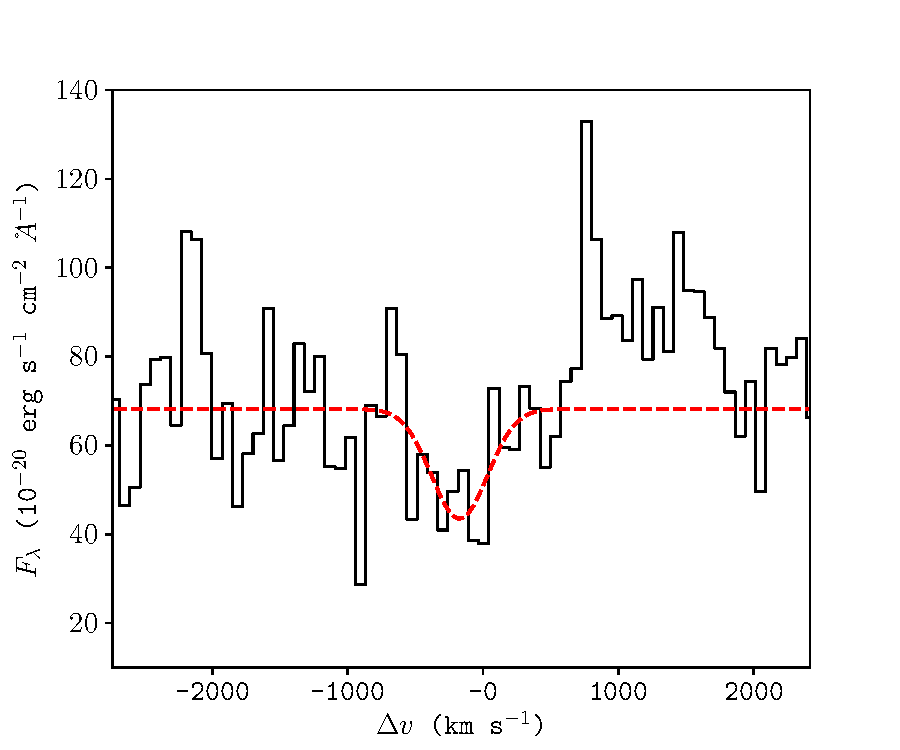
\includegraphics[width=0.75\textwidth]{plots_chp3/SiII_1260.pdf}
\caption[\ion{Si}{II} $\lam$1260 absorption line in MUSE and its best fit]{\ion{Si}{II} $\lam$1260 absorption line fit by a single Gaussian component (shown in red). }
\label{fig:SiII_1260-fit}
\end{figure}

\begin{figure}
\centering 
\includegraphics[width=0.75\textwidth]{plots_chp3/SiII_1526.pdf}
\caption[\ion{Si}{II} $\lam$1527 absorption line in MUSE and its best fit]{\ion{Si}{II} $\lam$1527 absorption line fit by a single Gaussian component (shown in red). }
\label{fig:SiII_1526-fit}
\end{figure}

\begin{figure*} 
\centering
 \includegraphics[width=0.75\textwidth]{plots_chp3/absorber_velocities.pdf}
 \caption[Velocity shifts of absorbers for resonant ions]{Relative velocities of Ly$\alpha,$ \ion{N}{V,} and \ion{C}{IV} and \ion{Si}{II} absorbers from this work as well as those from G16 and S18. The vertical dash-dotted (black) line indicates the systemic velocity and its error shown by the narrow shaded grey region. The horizontal dashed lines (grey) distinguish between the different absorbers.}
 \label{fig:abs-vel}
\end{figure*}

\subsection{\ion{C}{III]} and \ion{C}{ii]}}
The gas tracers \ion{C}{III]} $\lam\lam1906,1908$ and \ion{C}{II]} $\lam2326$ are non-resonant lines but useful tracers when searching for evidence of shock ionisation, which we discuss in more detail in section \ref{section:photoionisation-modelling}. We therefore included them in the line-fitting routine. To the \ion{C}{III]} doublet, we fit four Gaussian components in total to account for emission from the doublet at both systemic and blueshifted velocities as we have done for Ly$\alpha,$ \ion{He}{II,} and \ion{C}{IV}. \ion{C}{III]} has a sufficiently high surface brightness for us to fit it in the same way. Its best-fit result is shown in Fig. \ref{fig:CIII]-and-CII-fit}a. \ion{C}{II]} is a singlet that showed evidence of very blueshifted emission relative to systemic, and thus we also added an additional Gaussian component when fitting it (see Fig. \ref{fig:CIII]-and-CII-fit}b). The best-fit emission parameters for both of these lines are shown in Table \ref{table:emission-fits}.

\begin{figure} 
\centering
 \subfloat[]{\includegraphics[width=0.5\textwidth]{plots_chp3/CIII]_fit.pdf}}
 \subfloat[]{\includegraphics[width=0.5\textwidth]{plots_chp3/CII]_fit.pdf}}\\
 \caption[\ion{C}{III]} $\lam1906,1908$ and \ion{C}{II} $\lam 2326$ lines and their best-fits]{Panel (a): The \ion{C}{III]} $\lam1906,1908$ doublet line fit. Panel (b): The \ion{C}{II} $\lam 2326$ singlet line fit. Evidence for a blueshifted emission component is visible in both lines.}
\label{fig:CIII]-and-CII-fit}
\end{figure}


\section{Morphology of the absorbers}\label{section:morphology-absorbers}
The morphology of the absorbers within the circumgalactic medium of Yggdrasil is a focus of interest because much uncertainty about their origin and probable fate still remains, although the absorbers have been studied extensively using data from long-slit \citep[i.e.][]{rottgering1995,vanojik1997} and echelle spectroscopy \citep[i.e.][]{jarvis2003,wilman2004}, which were limited in their ability to provide a spatially resolved view of the gas in emission and absorption around Yggdrasil. In particular, they were not capable of showing the spatial variation in the \lya~profile that indicates variation in the kinematics of the most extended absorber (absorber 2). 

The MUSE data we used to perform resonant line-fitting above provide us with the capability of estimating the full extent and shape of \lya~absorber 2, which has a covering factor of C $\simeq$ 1.0, as G16 and S18 have shown. Furthermore, we can deduce its neutral and also ionised gas mass, and thus estimate its total hydrogen gas mass. 

\subsection{Size, shape, mass, and ionisation of the strongest \lya~absorber}\label{section:morphology}

In agreement with previous work on the \lya~line in Yggdrasil, absorber 2, located at a velocity shift of $\Delta \varv \sim-400$ km s$^{-1},$ reaches zero flux at its line centre. This implies that it is saturated with a unity covering factor, that is, C $\simeq$ 1.0 and \lya~column density of $\sim$ $10^{19}$ cm$^{-2}$ (see Table \ref{table:absorption-fits}). In the UVES spectrum, the \lya~absorbers occupy disparate velocities. This implies that the structure of the \ion{H}{I} gas is likely to be shell-like, as \citet{binette2000} and \citet{jarvis2003} have suggested. Guided by these previous findings and using more recent IFU data, we can estimate the size, shape, and mass of absorber 2, which is the strongest \lya~absorber. 

In terms of location, we relied on the result given in \citet{binette2000}, who showed that the absorbing and emitting gas are not co-spatial. Rather, absorber 2 is farther out of the halo and screens the radiation from the extended emission line region. We base the rest of our description of the halo gas on this predication. The spatial extent of the absorbing \ion{H}{I} gas medium in \citet{rottgering1995} is found to be $r \gtrsim 13$ kpc based on the extent of the measured \lya~emission and on the assumption of a unity covering factor for the associated absorption. In G16, visual inspection of the IFU data led to a value of $r \gtrsim 60$ kpc in radial extent. In S18, a velocity gradient across the halo was measured and used to estimate the absorber size, which the authors found to be $r \gtrsim 38$ kpc in radius. Here, we used the radial size of the \ion{H}{I} gas shell from G16, who determined the size by pinpointing the farthest spaxels from the nucleus of the gas halo at several position angles where the \lya~absorber 2 is still observed. 

In our data, we find that the absorber extends to projected distances of between $r = 50$ kpc and $r = 60$ kpc from the HSBR and is non-isotropic, covering the EELR over an area of 50 $\times$ 60 kpc$^{2}.$ A low surface brightness halo with quiescent kinematics (FWHM = 400 - 600 km s$^{-1}$) extending out to $r = 67$ kpc has been detected in this source \citep[e.g.][]{villar-martin2003}. Ly$\alpha,$ \ion{He}{II}, \ion{N}{V,} and \ion{C}{IV} emission are detected in the giant halo. In fact, \ion{N}{V} appears to be strengthened more than in the quiescent haloes of other HzRGs in \citet{villar-martin2003}. Given the size of the absorber, it is likely that it covers the emission from the giant halo. 

Assuming spherical symmetry and density homogeneity of the absorbing gas shell, the \ion{H}{I} mass is estimated to be $M_\ion{H}{I} = 4 \pi r^2 {\rm m}_\ion{H}{I} N_\ion{H}{I}$ \citep{deBreuck2003,humphrey2008b}. When we take into account the estimated size of $r \gtrsim 60$ kpc and an \ion{H}{I} column density of $10^{19.2}$ cm$^{-2}$ (from Table \ref{table:absorption-fits}), the \ion{H}{I} mass of absorber 2 is $M_\ion{H}{I}/\rm{M}_\odot = 5.7\e{9} (r / 60 {\rm kpc})^2$ $(N_\ion{H}{I} / 10^{19.2} {\rm cm}^{-2}).$ Our results agree to within at most two orders of magnitude with those in the literature. \citet{rottgering1995} estimated the mass of absorber 2  as $ M_\ion{H}{I}/\rm{M}_\odot \gtrsim 2.0\e{7} (N_\ion{H}{I} / 10^{19} {\rm cm}^{-2})(r / 13 {\rm kpc}).$ In G16, this value is $M_\ion{H}{I}/\rm{M}_\odot \gtrsim 3.8\e{9}(r / 60 {\rm kpc})^2$ $(N_\ion{H}{I} / 10^{19} {\rm cm}^{-2}), $ and the estimate given in S18 is $M_\ion{H}{I}/\rm{M}_\odot \gtrsim 10^{8.3}.$

An approximation of the hydrogen ionisation fraction X$_\ion{H}{II} = \ion{H}{II}/(\ion{H}{I}+\ion{H}{II})$ is clearly required to estimate the gas mass of the absorbing structure from our observational measurement of $N_\ion{H}{I}.$ In principle, the value of X$_\ion{H}{II}$ can vary from zero in the case of purely neutral gas to $\sim$1.0 in the case of matter-bounded photoionised gas \citep[e.g.][]{binette1996,wilson1997}. In the absence of a method for directly estimating N$_\ion{H}{II},$ we instead turn to the carbon ionisation fraction, X$_{\rm C}$, which we define here as the ratio of all ionised species of carbon to all species of atomic carbon (i.e. ionised or neutral). For Yggdrasil, we combined the measurement of $N_\ion{C}{IV}$ with the upper limit $N_\ion{C}{I}$ $\le$ 1.5 $\times$10$^{14}$ cm$^{-2}$ from S18 to obtain X$_{\rm C}$ $\ge$ $N_\ion{C}{IV} / (N_\ion{C}{I}+N_\ion{C}{IV}) = 0.8.$ 

This is a lower limit because we have no useful constraints on any of the other ionised carbon species. The fact that the ionisation energy of \ion{C}{I} (11.3 eV) is similar to that of \ion{H}{I} (13.6 eV) means that under photoionisation, we can assume that the ionisation fraction of hydrogen and carbon are similar, that is, X$_\ion{H}{II}$ $\sim$ X$_{\rm C},$ and thus we obtain X$_\ion{H}{II}$ $\gtrsim$ 0.8. This falls within the framework of the absorber being ionisation rather than matter bounded, as suggested by the \ion{Si}{II} detections in section \ref{section:SiII-fit}.  

The neutral fraction is what is remaining, that is, X$_\ion{H}{I} \lesssim 0.2.$ When we assume that the absorber is a two-phase medium as in \citet{binette2000}, the ionised fraction implies that $M_\ion{H}{II}/M_\ion{H}{I} \gtrsim 4.$ Using this, we can estimate the total hydrogen mass (excluding the molecular gas contribution) of the absorber such that it is $M_{\rm T}/\rm{M}_\odot \gtrsim M_\ion{H}{I} + M_\ion{H}{II} = 5 M_\ion{H}{I}$ , hence $M_{\rm T}/\rm{M}_\odot \gtrsim 2.9\e{10}.$ The mass of absorber 2 is approximately an order of magnitude lower than the stellar mass of the host galaxy, which is $M_*/\rm{M}_\odot = 1.2\e{11}$ \citep{seymour2007}. 

\subsection{Arrangement of the absorbers along the line of sight}\label{section:arrangement-absorbers}

Fig. \ref{fig:abs-vel} shows that \lya~absorption occurs in the same gas volume as absorbers 1, 2, and 3 in \ion{C}{IV}, \ion{N}{V,} and \ion{Si}{IV}. From the velocities of these absorbers, we can determine a) their geometric arrangement in the halo and b) their kinematics. Are these outflowing \citep[e.g.][]{zirm2005,nesvadba2006} or infalling gas \citep[e.g.][]{BarkanaLoeb2003,humphrey2008b}?

In agreement with general observations of HzRGs, \lya~absorbers 1 and 2 are blueshifted relative to the systemic velocity \citep{wilman2004}. According to velocity gradient measures across the diameter of the \lya~halo in S18, \lya~absorber 2 is outflowing. Assuming that absorbers 1, 2, and 3 are outflowing, we can estimate where they are located in relation to one another along the line of sight. At $\Delta \varv \sim-1000$ km s$^{-1},$ absorber 1 has the highest blueshift and is thus more likely to be found at a closer proximity to the nucleus than absorber 2, which is located at $\Delta \varv \sim-400$ km s$^{-1}.$ In other words, absorber 1 has the fastest outflow velocity and is therefore closer to the centre of the halo. Absorber 3 is redshifted relative to the systemic velocity, and it may be infalling. To measure the distances, we require simulated abundances produced by photoionisation models (shown in section \ref{section:photoionisation-modelling}). 

\section{Blueshifted \ion{He}{II}, Ly$\alpha,$ and \ion{C}{IV} emission}\label{method:blueshifted-emission}

The blueshifted components in the bright lines \ion{He}{II}, Ly$\alpha,$ and \ion{C}{IV} are a clear indication of perturbed gas either in the foreground of systemic emission in the halo or outflowing along the line of sight. To separate the blueshifted and systemic emissions in \ion{He}{II}, we used narrow-band imaging. A MUSE narrow-band image summed over a wavelength range of $6400 - 6425$ $\ang$ is shown as contours in Fig. \ref{fig:hst-img-muse-contours}. We note that the contours are continuum-free. Within this chosen wavelength range, we obtain detections from the blueshifted and systemic \ion{He}{II} emitters. The image clearly shows two spatially unresolved components: one at the high surface brightness peak, and the other spatially offset. 

In addition to this spatial separation, the \ion{He}{II} spectra extracted from each of these two regions show that emission in the HSBR (shown in Fig. \ref{fig:0943-continuum}) is dominated by emission from the systemic velocity; trace amounts are blueshifted. The blueshifted component, however, undergoes a flux enhancement by an approximate factor of 2 (see Table \ref{table:HeII-nucleus-offset}) at a projected distance of $d = 1.00 \pm 0.04 \arcsec = 8.0 \pm 0.3$ kpc south-west (PA $\simeq 225^\circ$) from the HSBR. 

For further understanding, we show the MUSE \ion{He}{II} contours over a UV/optical {\it Hubble Space Telescope} (HST) Wide Field Planetary Camera 2 (WFPC2) 702W broad-band image. The UV emission detected over $5800 - 8600$ $\ang$ appears to have a bent morphology that extends in the same direction as the region where \ion{He}{II} is enhanced. Moreover, the UV broad-band detection and the blueshifted \ion{He}{II} are both aligned with the radio axis detected by 4.7 GHz Very Large Array (VLA) observations \citep{carilli1997,pentericci1999}. 

\begin{figure*}
\centering
\hspace*{-50pt}
\includegraphics[width=1.2\textwidth]{plots_chp3/HeII_nucleus_offset_NB_img.jpg}
\caption[HST rest-UV image overlaid with MUSE \ion{He}{II} and VLA 4.7 GHz contours]{Broad-band image of the rest-UV continuum of MRC 0942-242 from the {\it HST} WFPC2 702W ($5800 - 8600$ $\ang$) filter. MUSE contours (blue) are overlaid and represent narrow-band emission summed over $6400 - 6425$ $\ang.$ The contours are shown at the surface brightness levels, (1.0, 1.6, 2.2, 2.8, 3.4, 4.0) $\times 10^{-17}$ erg s$^{-1}$ cm$^{-2}$ $ {\rm arcsec}^{-2}.$ VLA 4.7 GHz radio surface brightness is shown by the red contour levels. The inset 1D spectra show the HSBR ($left$) and offset ($right$) \ion{He}{II} emission. The line profiles are extracted from apertures of radius R = 0.6\arcsec, shown in green for the HSBR and in cyan for the offset region. The aperture centroids for each are shown in matching colours. The blueshifted and systemic \ion{He}{II} emissions are shown in blue and orange, respectively, and the sum of both components is shown in red. }
\label{fig:hst-img-muse-contours}
\end{figure*}

Obtaining a narrow-band image over a smaller wavelength range of $6400 - 6412$ $\ang$ (blue interval in Fig \ref{fig:0943-emission}(d)) allows us to distinguish the blueshifted \ion{He}{II} emission from the \ion{He}{II} emission at the systemic velocity. \ion{He}{II} emission from the blueshifted component alone is shown in Fig \ref{fig:0943-emission}(a), which proves that emission from the blue wing of the \ion{He}{II} line is indeed spatially offset from the HSBR.

\ion{The He}{II} emission at the systemic velocity is less highly concentrated. Over the green interval in Fig. \ref{fig:0943-emission}(d), \ion{He}{II} is diffuse and elongated well beyond the radio lobes, indicating possible jet-gas interactions. At the red wing of the line, \ion{He}{II} emission is concentrated in the eastern lobe and HSBR, as Fig. \ref{fig:0943-emission}(c) shows. 

Both \lya~and \ion{C}{IV} show evidence for turbulent blueshifted motions in the line-fitting (see sections \ref{section:Lya-fit} and \ref{section:CIV-NV-fit}). If the blueshifted component is indeed an outflow, this implies that the outflowing gas contains more than one ionised gas tracer, which we can expect for a bulk outflow of gas from the enriched ISM. 

\begin{sidewaystable}
\caption[Best-fit \ion{He}{II} emission line results]{Best-fit results to \ion{He}{II} HSBR and offset lines in Fig. \ref{fig:hst-img-muse-contours}. The emission is also classified as blueshifted relative to the systemic velocity or is emitted from the systemic velocity.}    
\centering                          
\begin{tabular}{ l l D{,}{\, \,\pm\, \,}{-3} D{,}{\, \,\pm\, \,}{-3} D{,}{\, \,\pm\, \,}{-3} D{,}{\, \,\pm\, \,}{-3} }
\hline\hline MUSE  \\
\hline            
\ion{He}{II}$\lambda1640$ line region  
& Component 
& \mc{Line centre (obs.)} 
&\mc{Line flux}  
& \mc{Line width}
& \mc{Velocity}   \\ 
&  
& \mc{$\lam$ (\ang)} 
& \mc{$F$ (10$^{-17}$ erg s$^{-1}$ cm$^{-2}$)}
& \mc{FWHM (km s$^{-1}$)} 
& \mc{$\Delta \varv$} \\  
&  &  & \mc{} & \mc{} &\mc{} \\  
\hline     
&  &  & \mc{} & \mc{} &\mc{} \\  
HSBR    & blueshifted   & 6413.49,3.04   & 1.43,0.47       & 970, 225       & -1053,3206  \\  
              & systemic       & 6436.09,0.30  & 16.42,4.86    & 978, 24         & 0.02,0.01 \\ 
&  &  & \mc{} & \mc{} &\mc{} \\                                  
Offset  & blueshifted     & 6414.18,3.21  & 2.69,0.81                & 1134, 195     & -1025,3251\\  
            & systemic        & 6434.76,0.83  & 7.64,0.80             & 993,48          & -46,27 \\   
&  &  & \mc{} & \mc{} &\mc{} \\   
\hline                                   
\end{tabular} 
\label{table:HeII-nucleus-offset}  
\end{sidewaystable}

\begin{figure}
\hspace*{-50pt}
\centering
        \subfloat[\ion{He}{II} blueshifted: $6400 - 6412$ $\ang;$ blue interval in Fig. \ref{fig:0943-emission}(d)]{\includegraphics[width=0.6\textwidth]{plots_chp3/HeII_blue_VLA_arcsec.pdf}}
        \subfloat[\ion{He}{II} diffuse: $6425 - 6430$ $\ang;$ green interval in Fig. \ref{fig:0943-emission}(d)]{\includegraphics[width=0.6\textwidth]{plots_chp3/HeII_green_VLA_arcsec.pdf}}\\
\hspace*{-50pt}
        \subfloat[\ion{He}{II} redshifted: $6445 - 6450$ $\ang;$ red interval in Fig. \ref{fig:0943-emission}(d)]{\includegraphics[width=0.6\textwidth]{plots_chp3/HeII_red_VLA_arcsec.pdf}}
        \subfloat[\ion{He}{II} line emission]{\includegraphics[width=0.5\textwidth]{plots_chp3/HeII_profile.pdf}}
\caption[MUSE \ion{He}{II} narrow-band images]{MUSE continuum-subtracted narrow-band images showing the spatial variation in \ion{He}{II} emission at different wavelength bands. The green and cyan crosses show the centres of the HSBR and offset \ion{He}{II} emission from which the line profiles in Fig. \ref{fig:hst-img-muse-contours} are extracted. The 4.7 GHz VLA radio contours are shown in red at the levels $3\sigma,$ $3\sqrt{2}\sigma,$ $9\sqrt{2}\sigma,$ and $15\sqrt{2}\sigma$ for $\sigma = 2\e{-5}$ Jy beam$^{-1}$. Panel (a): The blueshifted component is detected over $6400 - 6412$ $\ang$ in the blue interval and is shown as a narrow-band image. In this figure, the sub-structure of the emission is also shown using MUSE \ion{He}{II} contours with surface brightness levels (0.038, 0.079, 0.120) $\times 10^{-17}$ erg s$^{-1}$ cm$^{-2} {\rm arcsec}^{-2}$ in yellow. Panel (b): The diffuse \ion{He}{II} gas, represented by the green spectral range, that is, $6425 - 6430$ $\ang,$ extends in the direction of the south-western lobe. Panel (c): In the red spectral interval, that is, $6445 - 6450$ $\ang,$ a redshifted component that has a clear spatial association with the north-eastern radio lobe is visible. The velocity intervals for these narrow-band images are displayed in the \ion{He}{II} profile in Panel (d), which is a spectrum extracted from an aperture centred on the HSBR over a radius of R = 0.6\arcsec. }
\label{fig:0943-emission}
\end{figure}

\section{Quasar and HzRG absorbers, in comparison}\label{section:hzrg-vs-quasar-abs}
The absorption lines in a quasar continuum emerge from absorption by intervening gas in the IGM and the CGM of a foreground galaxy \citep[e.g.][]{bechtold2001}. Here,we used quasar absorption lines to determine whether the absorbers in Yggdrasil are associated with the halo of the galaxy or the IGM, assuming that HzRG and quasar absorbers are drawn from the same parent population. 

To do this, we compared our results to quasar absorption parameters of \ion{H}{I}, \ion{N}{V,} and \ion{C}{IV} for associated quasar absorbers from \citet{fechner2009}. In this work, the absorbing gas identified as intervening is located at velocity shifts of $\lvert \Delta \varv \rvert > 5000$ km s$^{-1}$ from the quasars in their sample. The  associated absorbers are those at velocity shifts $\lvert \Delta \varv \rvert > 5000$ km s$^{-1}$ from the quasars. We show this comparison in Fig \ref{fig:NV-quasar-absorption}. Our results (which generally have velocity shifts $\lvert \Delta \varv \rvert < 1500$ km s$^{-1}$ for all absorbers) agree better with absorption by associated than by intervening gas. This implies that the absorbers in Yggdrasil are more likely to be associated with the galaxy, that is, the absorbers are bound to the ISM and/or CGM if they are similar or from the same parent distribution.

We have an additional set of quasar absorbers with which to compare the \ion{C}{IV} and \ion{Si}{IV} column densities we measured. Quasar absorption for the ionised gas, in particular, has been measured by \citet{songaila1998} and \citet{dodorico2013}. In the former, absorption is from the IGM, while the latter results show quasar-associated absorption at much higher redshifts of z $>$ 6. This comparison is shown in Fig. \ref{fig:SiIV-quasar-absorption}. This figure shows that Yggdrasil absorbers agree better with the associated absorbers of \citet{dodorico2013} than with the intervening absorbers of \citet{songaila1998}. These order-of-magnitude comparisons show that the absorbers in the Yggdrasil spectrum are much more likely to be associated with the galaxy halo.

\begin{figure} 
\captionsetup[subfigure]{labelformat=empty}
\hspace{1pt}
\centering
\subfloat[Comparison with associated quasar absorption]{\includegraphics[width=0.55\textwidth]{plots_chp3/NV_associated_QSO_HzRGs.pdf}}
\centering
\subfloat[Comparison with intervening quasar absorption]{\includegraphics[width=0.55\textwidth]{plots_chp3/NV_intervening_QSO_HzRGs.pdf}}
\caption[$N_\ion{C}{IV}$ and $N_\ion{N}{V}$ column densities of host galaxy and quasar absorbers]{\ion{N}{V} and \ion{C}{IV} column densities of associated (left) and intervening (right) absorbers from \citet{fechner2009} (in grey and blue: secondary detections for the quasar) and Yggdrasil detections (red).}
 \label{fig:NV-quasar-absorption}
\end{figure}

\begin{figure} 
\centering
\includegraphics[width=0.55\textwidth]{plots_chp3/SiIV_CIV_QSO_HzRGs.pdf}
\caption[$N_\ion{C}{IV}$ and $N_\ion{Si}{IV}$ column densities of host galaxy and quasar absorbers]{$N_\ion{C}{IV}$ relative to $N_\ion{Si}{IV}$ for absorbers in the IGM in \citet{songaila1998} and those directly associated with the quasars \citep{dodorico2013}.}
\label{fig:SiIV-quasar-absorption}
\end{figure}

\section{Photoionisation modelling}\label{section:photoionisation-modelling}
We used a photoionisation modelling code to determine the main ionising mechanisms that produce the observed ionised gas and its column densities in the absorbing gas shells surrounding Yggdrasil. A very detailed study of this has been carried out by \citet{binette2000}, who obtained a metallicity of Z/Z$_\odot \simeq 0.02$ (Z$_\odot$ being the solar metallicity) for the strongest \lya~absorbers. Their findings also indicated that emitting and absorbing gas are not co-spatial and that the gas is best described by an \ion{H}{I} volume density of n$_\ion{H}{I} = 100$ cm$^{-3}.$ In addition to this, \citet{binette2006} sought to determine the ionising mechanism behind the absorbers in this source, and thus showed that stellar photoionisation results in the \ion{H}{I} and \ion{C}{IV} absorber column densities 

It is worth noting that their conclusions were obtained using only column densities for \ion{H}{I} and \ion{C}{IV}. With our recent detection of \ion{N}{V} absorption at the same velocity as the the strong \lya~absorber, we can provide more insight to these findings. Given the detection of \ion{N}{V}, flux from the meta-galactic background may be too weak to ionise the absorbers. At z $\geq$ 2.7, \ion{He}{II} reionisation was more active than it is at lower redshifts, meaning that ionising photons with energies of $E_\gamma > 54.4$ eV had megaparsec-scale mean free paths \citep{shull2010,mcquinn2016}. The meta-galactic background is therefore less likely to be a strong ionising mechanism powering the absorbers in the halo of Yggdrasil. 

We also considered the possibility that shocks by the powerful radio jets may ionise the gas. This was proposed by \citet{dopita1995}, and observational evidence for shock ionisation in HzRGs has been shown by several authors, particularly in sources with relatively small radio sources that are still contained within the host galaxy \citep[e.g.][]{allen1998,best2000a,debreuck2000}. A powerful diagnostic of shock-ionised emission are the line ratios of carbon: in shock ionised regions, we expect the \ion{C}{II]} $\lam2326$ line to be as strong as its higher ionisation counterparts. Our MUSE spectrum (Fig. \ref{fig:0943-spectrum}) contains three carbon lines and allows us to make this test. Interestingly, the \ion{C}{II]} $\lam1906,1908$ line contains a much stronger blueshifted component than the \ion{C}{III]} and \ion{C}{IV} $\lam\lam1548,1550$ lines. These high \ion{C}{II]}/\ion{C}{III]} and \ion{C}{II]}/\ion{C}{IV} ratios are consistent with shock ionisation \citep[see e.g. Fig. 1 of][]{best2000a}. This provides evidence to our claim that this blueshifted gas near the western radio lobe is an outflow driven by the radio jet. On the other hand, the radio of the main component near the AGN has a \ion{C}{III]}/\ion{C}{II]} ratio of $\sim$2.4, which places it squarely in the AGN photoionisation region. This main velocity component dominates the flux of all the other emission lines, therefore we did not consider shock ionisation as a relevant contributor in those lines.

Stellar photoionisation is a possibility as well. The star formation rate (SFR) in Yggdrasil, however, is SFR=41 M$_\odot$ yr$^{-1}$ \citep{falkendal2019} and may be insufficient to produce the starburst activity that would ionise the absorbers. Another possibility is the AGN, which we can expect to produce a strong enough ionising continuum to produce the detected absorption. 

We therefore revisited the analysis by running photoionisation models using \pkg{cloudy c17} \citep{ferland2017}, a spectral synthesis code designed to run grid models that provide simulated chemical abundances in photoionised gas. Within the halo of Yggdrasil, we have shown that \lya~absorbers are at the same velocity as \ion{C}{IV}, \ion{N}{V,} and \ion{Si}{IV} absorbers, suggesting that the gas tracers occupy the same gas volume. 

The ionisation parameter is defined as $U(r) = \frac{ 1 }{ 4 \pi {\rm r}^2 {\rm c} {\rm n}_\ion{H}{I}} \int^\infty_{\nu_0} \frac{ {\rm L}_\nu }{ h\nu }d\nu,$ is the quotient of the volume density of hydrogen-ionising photons and the volume density of hydrogen atoms contained within the gas. Here, $r$ is the line-of-sight distance from the ionising source to the gas, n$_\ion{H}{I}$ is the hydrogen density, $L_\nu$ is the specific luminosity, and $\nu$ is the observing frequency such that the integral, $\int^{\infty}_{\nu_0} \frac{ {\rm L}_\nu }{ h\nu }d\nu,$ is the luminosity of the ionising source. Provided that we can determine $U(r)$ for the radiation field ionising the absorbing gas, we can also compute the distance of the gas from the radiation source  along the line of sight.

\subsection{AGN photoionisation of the absorbers}\label{section:photoionisation-absorbers}

We have shown in the comparison to quasar absorbers in \citet{fechner2009} that the absorbers in Yggdrasil are located within the CGM rather than IGM. In the \pkg{cloudy} model, we used a power law spectral energy distribution \pkg{(SED;} where the ionising flux is given by S$_\nu \propto \nu^\alpha$) to simulate the incident radiation produced by the AGN. In this, we tested $\alpha=-1.5$ and $\alpha=-1.0$ to model the photoionisation of the gas by an AGN \citep[e.g.][]{villar-martin1997,feltre2016,humphrey2018}.

The model grid consists of a set of input parameters. The hydrogen density was fixed to n$_\ion{H}{I} = 100 {\rm cm}^{-3}$ , which is commonly adopted to describe the low-density diffuse gas that we expect in the extended absorbers \citep[e.g.][]{binette2000,humphrey2008a}. The metallicity (Z) was varied over a range of values between Z/Z$_\odot$ = 0.01 and 10. The \ion{H}{I} column density N$_\ion{H}{I}$ was taken from the line-fitting results (shown in Table \ref{table:absorption-fits}). The ionisation parameter varied over the range $ 10^{-2.5} < U < 10^{-1}$ in 0.5 dex increments.

We did not include the effects of dust extinction because the surface brightness of emission re-radiated by dust, detected by the Atacama Large Millimetre/sub-mm Array (ALMA) at an observing frequency of $\nu_{\rm obs}$ = 235 GHz is lower in Yggdrasil than in the offset region at projected distances of $d = 65$ to 80 kpc from the host galaxy, where three resolved dusty companions are observed (G16). This observation implies that dust has a negligible contribution to the \pkg{SED} at the host galaxy. Moreover, \citet{falkendal2019} have shown that the SFR in Yggdrasil is lower than that which is detected in the companion sources, collectively. 

In the \pkg{cloudy} models, we have assumed an open or plane-parallel geometry for the absorbing gas medium, which implies that the cloud depth is significantly smaller than its inner radius, or more simply, the distance between the ionising continuum source and the illuminated gas surface. Following the findings from \citet{binette2000}, we assumed that the absorbers are not co-spatial with the emitting gas. 

The column density measures we obtain are shown against the simulated column densities in Figs. \ref{fig:cloudy-abs1} and \ref{fig:cloudy-abs3}, and the results indicate that absorbers 1 and 3 may have supersolar metallicities of Z/Z$_\odot \simeq$ 10 and 5, respectively. However, due to uncertainties in line-fitting, the column densities obtained are upper limits and no proper conclusion can be drawn about the metallicities of the absorbers. If these models were to suggest super-solar metallicity in absorbers, this would not be unusual given that super-solar metallicities in HzRG absorption line gas have been measured before \citep{jarvis2003,binette2006}. \citet{jarvis2003} showed that absorbers in the halo of the z=2.23 radio galaxy, 0200+015, had Z/Z$_\odot \sim$ 10 and covering factors of C $<$ 1.0. This implied that the absorbers are likely to be co-spatial with the EELR. Based on Fig. \ref{fig:cloudy-abs2}, the measured column densities of absorber 2 prove that its metallicity is closer to a value of Z/Z$_\odot = 0.01.$  The results also suggest that the \ion{N}{V} column density is under-predicted by the Z/Z$_\odot = 0.01$ model. We explore the possible reasons for this in the following section. 

\begin{figure}
\centering 
\includegraphics[width=0.7\textwidth]{plots_chp3/0943_agn_photoion_CIV_NV_HI_abs1_hden_2.pdf}
\caption[Absorber 1: \pkg{cloudy} photoionisation predictions]{\ion{N}{V} and \ion{C}{IV} column densities obtained from \pkg{cloudy} photoionisation models. The predicted column densities are for absorber 1, which has an \ion{H}{I} column density of $N_{\ion{H}{I}} = 10^{14.2}$ cm$^{-2}$ that is kept constant as $U(r)$ increases from $U=10^{-2.5}$ to $U=10^{-1}$ in increments of 0.5 dex. The metallicities Z/Z$_\odot$ = 0.1, 0.5, 1, and 5 are tested for spectral indices $\alpha=-1.0$ (solid lines) and $\alpha=-1.5$ (dashed lines).}
\label{fig:cloudy-abs1}
\end{figure}

\begin{figure}
\centering
\includegraphics[width=0.7\textwidth]{plots_chp3/0943_agn_photoion_CIV_NV_HI_abs3_hden_2.pdf}
\caption[Absorber 2: \pkg{cloudy} photoionisation predictions]{\ion{N}{V} and \ion{C}{IV} column densities obtained from \pkg{cloudy} photoionisation models similar to those in Fig \ref{fig:cloudy-abs1}. The models shown here are for absorber 3 because the \ion{H}{I} column density is kept constant at $N_{\ion{H}{I}} = 10^{13.3}$ cm$^{-2}.$ The metallicities tested are Z/Z$_\odot$ = 0.1, 0.5, 1, and 5.}
\label{fig:cloudy-abs3}
\end{figure} 

\begin{figure}
\centering
\includegraphics[width=0.7\textwidth]{plots_chp3/0943_agn_photoion_CIV_NV_HI_abs2_hden_2.pdf}
\caption[Absorber 3: \pkg{cloudy} photoionisation predictions]{\ion{N}{V} and \ion{C}{IV} column densities obtained from photoionisation \pkg{cloudy} models similar to those in Fig. \ref{fig:cloudy-abs1}. The models shown here are for absorber 2, the strong absorber, because the \ion{H}{I} column density is kept constant at $N_{\ion{H}{I}}$ = $10^{19.2}$ cm$^{-2}.$ The nitrogen abundance at Z/Z$_\odot = 0.01$ has also been enhanced by a factor of 10 (orange curve) i.e. N/C = 10.}
\label{fig:cloudy-abs2}
\end{figure}

\subsection{Nitrogen abundances under-predicted by AGN photoionisation}

The assumed power laws for the ionising continuum do not reproduce the metal ion column densities observed in the strong absorber (absorber 2). We are certain that the \ion{C}{IV} column density is well measured, given its agreement to literature values (\citealp{jarvis2003}; G16). The \ion{N}{V} cannot be compared to any previous results other than the quasar absorbers shown in Fig. \ref{fig:NV-quasar-absorption}, but has been fit with a similar level of uncertainty as \ion{C}{IV}. The results shown in Fig. \ref{fig:cloudy-abs2} indicate that AGN photoionisation alone cannot produce the measured \ion{N}{V} column densities. At the same time, a softer ionising continuum is also insufficient in producing a high-ionisation tracer such as \ion{N}{V}. In other words, a power law under-predicts the measured \ion{N}{V} column density for the strong \lya~absorber. We therefore explored secondary nitrogen production, enhanced nitrogen abundances, and a lower \ion{H}{I} column density as possible reasons for under-predicted nitrogen abundances. 

\subsubsection{Secondary nitrogen production}

The under-predicted nitrogen abundance may result from scaling the nitrogen abundance (relative to hydrogen) according to the solar value, that is, N/C $\propto$ (N/C)$_\odot.$ We propose secondary nitrogen production by intermediate-mass stars with M/M$_\odot=$ 1 - 8 \citep[e.g.][]{henry2000}. In this process, abundances scale as N/O $\propto$ O/H $\propto$ Z (with N, O, and H being the nitrogen, oxygen, and hydrogen abundances and Z the metallicity of the gas). This implies that N/C $\propto$ (O/H)$^2$ $\propto$ Z$^2.$ However, secondary nitrogen production is known to occur in gas with super-solar metallicities (i.e. Z/Z$_\odot \geq 1.0$) while primary nitrogen production dominates at sub-solar metallicities \citep[e.g.][]{Hamann&Ferland1993}. We can consider secondary nitrogen the cause of nitrogen enhancement in absorber 2. Fig. \ref{fig:NV-quasar-absorption}(a) shows that the absorbers in Yggdrasil have similar column densities as associated quasar absorbers in the \citet{fechner2009} sample. In this study, secondary nitrogen production is posited as a reason for the nitrogen enrichment of the quasar absorbers.  

If secondary nitrogen production from carbon and oxygen in the CNO cycle were to cause the enhanced nitrogen abundance in the strong absorber, the absorber would have a higher metallicity than originally determined \citep[Z/Z$_\odot \simeq 0.02$;][]{binette2000,binette2006}. As is the case for the EELR in S18, where it is said to occur, secondary nitrogen production occurs for a gas metallicity of Z/Z$_\odot \simeq 2.0.$ The \pkg{cloudy} model grid indicates that in order for gas to be enriched by secondary nitrogen, it would also have a metallicity of Z/Z$_\odot \geq 1.0.$ This is improbable given that an increase in the cloud metallicity results in an increase in both the \ion{C}{IV} and \ion{N}{V} column densities. We therefore exclude secondary nitrogen production as a mechanism for the enhancement of nitrogen abundances. 

\subsubsection{Degeneracy of $b$ and N$_\ion{H}{I}$ for the strong absorber}

The degeneracies between the \ion{H}{I} column density $N_\ion{H}{I}$ and the Doppler parameter have been described in S18, who found two probable best-fit solutions for the $b$ parameter and N$_\ion{H}{I}$ in absorber 2. These are $N_\ion{H}{I}/{\rm cm}^{-2} = 10^{19.63}$ with $b = 52$ km s$^{-1}$ and $N_\ion{H}{I}/{\rm cm}^{-2} = 10^{15.20}$ with $b = 153$ km s$^{-1}.$ Taking the lower \ion{H}{I} column density solution as well as the $N_\ion{C}{IV}$ and $N_\ion{N}{V}$ measurements from our results, we ran the \pkg{CLOUDY} model grid using the same AGN photoionisation scheme (described in section \ref{section:photoionisation-absorbers}).

This time, applying the low \ion{H}{I} column density solution (i.e. $N_\ion{H}{I}/{\rm cm}^{-2} = 10^{15.20}$) to the grid resulted in the observed column density ratios (i.e. $N_\ion{C}{IV}/N_\ion{H}{I}$ and $N_\ion{N}{V}/N_\ion{H}{I}$), suggesting that absorber 2 has a supersolar metallicity, Z/Z$_\odot \simeq 5.$ This result differs greatly from the expected abundances from \citet{binette2000}, that is, Z/Z$_\odot \simeq 0.02,$ which was obtained through photoionisation modelling in \pkg{MAPPINGS IC} \citep{binette1985,ferruit1997}. This result may imply that if the cloud had a lower \ion{H}{I} column, its metallicity would need to be higher than Z/Z$_\odot \simeq 0.01.$ 

\subsubsection{Nitrogen abundance enhancement}

For the \pkg{cloudy} models to reproduce the observed column densities, we require a nitrogen abundance that is greater than the solar abundance by a factor of 10, as Fig. \ref{fig:cloudy-abs2} suggests. We can examine occurrences of enhanced nitrogen abundances in similar sources to attempt to find an answer for this. 

The photoionisation models shown in Fig. 10 of \citet{binette2006} seem to suggest that the \ion{N}{V} column density of absorber 2 may be ionised by the same mechanism that ionises the Lynx arc nebulae, which is a metal-poor \ion{H}{II} galaxy at z $\simeq$ 3.32 that has undergone a recent starburst \citep{villar-martin2004}. However, this scenario would require stellar photoionisation rather than an AGN. The presence of \ion{N}{V} in the absorber presents a strong case for an AGN rather than stellar photoionisation because it has such a high ionisation energy. 

To determine whether the current episode of AGN activity has ionised the absorber, we determined its lifespan. The radio size of Yggdrasil is $r \simeq$ 29 kpc \citep{pentericci1999}, and its approximate expansion speed is $\varv \simeq$ 0.05c. The age of the radio source therefore is approximately $\tau_{\rm jet} \simeq$ 2 Myr. The strong absorber, on the other hand, is roughly $r \simeq$ 60 kpc, and has an outflow rate of 400 km s$^{-1}$ relative to the galactic nucleus. This translates into an approximate outflow time-scale of $\tau_{\rm abs} \simeq 200$ Myr. That the radio source is a factor of 100 younger than the absorber implies that the current duty cycle of the radio jet can be responsible for the ionisation of the absorber, but it did not eject the gas that formed absorber 2. 

% explain feedback and enrichment scenario and possibility of stellar wind instead of AGN
To explain the chemical abundances, we propose that the absorber has been enriched by an early episode of star formation. Metal-rich gas from the ISM is driven by starbursts and through powerful winds, which dilutes the low-metallicity gas in absorber 2. Evidence of this is seen in local massive ellipticals, which are considered the progeny of HzRGs, where nitrogen abundances are enhanced well above that of carbon, that is, [N/Fe] $\sim 0.8-1$ and [C/Fe] $\sim$ 0.3 (for nitrogen, N, carbon, C, and iron, Fe, abundances) as a result of starburst-driven superwinds \citep{greene2013,greene2015}. 

\subsection{Distances of absorbers from the ionising source}

\begin{figure} 
\centering
\includegraphics[width=0.8\textwidth]{plots_chp3/0943_absorption_schematic8.pdf}
\caption[Cross-section schematic of the circumgalactic medium of MRC 0943-242]{Cross-section schematic of the circumgalactic medium of Yggdrasil based on evidence from the MUSE data and previous measures. The gas has no defined spatial boundaries because its estimated size of d $\gtrsim$ 60 kpc is merely a minimum. The strong absorber screens emission that originates from the T $\simeq10^4-10^6$ K EELR gas (in yellow), comprising an extended region of ionised gas as well as gas that is directly ionised by the AGN ionisation cone (in red). The absorbing gas (shown as dotted curve) is also metal enriched, as shown by \ion{C}{IV}, \ion{N}{V,} and \ion{Si}{IV} that are detected at the same velocities as the \lya~absorption. The blueshifted component detected in \lya~and \ion{He}{II} is a jet-induced outflow (blue arrows). This outflowing, ionised, and turbulent gas is spatially offset from the HSBR of the halo, which implies that the radio jet is tilted relative to the projected plane. The location of absorber 2 is at a line-of-sight projected distance, which is dependent on the ionisation parameter, $U(r).$}
\label{fig:absorption-cartoon}
\end{figure}

The distance between the AGN and the absorbing gas can be estimated but is dependent on n$_{\ion{H}{I}}.$ Given that we cannot constrain the hydrogen density, we have only the ratio of ionisation parameters to infer the distance ratios of two absorbers, for instance, $r_2 / r_1 = \sqrt{U_1 / U_2}.$ Assuming that the \ion{H}{I} gas volume density of n$_\ion{H}{I} = 100$ cm$^{-3}$ is correct, we can approximate the distance of absorber 2 from the AGN using the integrated infrared luminosity, $L_{\rm IR}^{\rm AGN},$ of the host galaxy computed by \citet{falkendal2019}. According to Fig. \ref{fig:cloudy-abs2}, the ionisation parameter for absorber 2 is approximately $U \simeq 10^{-2.25}.$ Expressing the ionisation parameter as $U(r) = L/n_\ion{H}{I}r^2$ \citep[e.g.][]{rozanska2014}, we obtain a distance of $d \simeq 68^{+17}_{-14}$ kpc between absorber 2 and the AGN.

%---------------------------------------------------------------------------------------------------------------------------------------------------

\section{Discussion}\label{section:discussion}
\subsection{Blueshifted emission: companion galaxy or outflow?}\label{discussion:blueshifted-emission}

There is sufficient evidence to suggest that the preferred environments of radio galaxies are rich clusters and groups. This is at low redshifts (z $\lesssim$ 1), where the most radio-loud sources have a higher likelihood of residing in Mpc-scale overdense structures \citep[e.g.][]{best2007,karouzos2014a,magliocchetti2018,kolwa2019a}. Radio-loud sources are also prevalent in over-dense environments consisting of dusty starburst galaxies and/or \lya~emitters at z $>$ 1.2 \citep[e.g.][]{hatch2011,wylezalek2013,dannerbauer2014,saito2015}. Based on these findings, we hypothesise that the blueshifted emission in this source may stem from a proto-galaxy or dwarf satellite.

A well-studied example is a Minkowski's object, associated with the radio galaxy PKS 0123-016, which has an increased SFR due to the passage of the radio source's jets \citep{vanbreugel1985}. The high-velocity dispersions of the blueshifted emission in Yggdrasil imply a different origin of the gas. Only an AGN would produce the turbulent gas motions that can broaden lines such as \ion{He}{II} to line widths of FWHM=1500 km s$^{-1}.$ Furthermore, dwarf galaxies tend to have outflow velocities of ionised gas of $\varv_{\rm out} \lesssim 100$ km s$^{-1}$ \citep{martin2005}. Such velocities are well below the outflow rates we observe in the blueshifted ionised gas, where the velocities are $\varv_{\rm out} \gtrsim 400$ km s$^{-1}$. 

It is more likely that the gas turbulence is driven by the jets. This is also a known occurrence within the gas haloes of powerful radio galaxies \citep[e.g.][]{humphrey2006,morais2017,nesvadba2017a}. The jet-driven outflow scenario is well supported in 4.7 GHz radio observations that indicate from rotation measures that radio emission from the western radio lobe in this source propagates over a shorter path length than radio emission from the eastern lobe \citep[e.g.][]{carilli1997}. 

This configuration implies that the radio axis is also tilted at a non-zero inclination angle with respect to the projected plane, as shown Fig. \ref{fig:absorption-cartoon}. If the jets were parallel to the plane of the sky, we would observe similar rotation measures at both the east and west radio lobes. The rotation measure at the eastern lobe is higher than that at the western lobe. This jet inclination can also explain that the blueshifted emission is an outflow.

%It represents AGN photoionised outflowing gas that is jet-driven or perturbed as has been identified by \citet{villar-martin2003}. In that work, the high-surface brightness \ion{He}{II} emission was measured with line widths of FWHM $\sim$ 1600 km s$^{-1},$ which indicates perturbed gas kinematics in the extended emission line region (EELR). The perturbed emitting gas is also seen to have a close alignment with the radio jet axis as has been observed for several other HzRGs \citep[e.g.,][]{vanojik1996,humphrey2006}. 

The kinematics surrounding the jet-gas interactions in the gas halo of Yggdrasil have been measured in previous studies. \citet{villar-martin2003} reported that the narrow components of \ion{He}{II} emission were blueshifted from the systemic at velocity shifts of $\Delta \varv \sim$ 100 km s$^{-1}.$ This kinematically quiet component identified as having a FWHM $\sim$ 500 km s$^{-1}$ is shown to extend across the entire halo, well beyond the radio hotspot. This suggests jet-gas interactions. In addition to this, \citet{humphrey2006} found that the \ion{He}{II} gas that has a perturbed component with FWHM = 1760 km s$^{-1}$ and the quiescent component with FWHM = 750 km s$^{-1},$ respectively, at a velocity shift of $\Delta \varv \sim$ -250 km s$^{-1}$ is low-ionisation gas. We here find that the blueshifted emission has FWHM = 970 km s$^{-1}$ at $\Delta \varv \sim$ -1000 km s$^{-1}.$ Although our measured velocity shifts differ slightly from those of previous works, the common thread is that the \ion{He}{II} emission is blueshifted relative to systemic and aligned with the radio axis. This indicates jet-gas interactions.  

This view agrees well with observations from G16, who reported direct evidence for the ionisation cone to be projected along the radio jet axis in the form of extended \ion{He}{II}, \ion{C}{IV} and \ion{C}{III]} emission to the south-west of the source. A detailed discussion of the ionised gas kinematics is presented in S18. Their interpretation differs from ours only slightly in that our radio axis is tilted relative to the projected plane. 

In addition to \ion{He}{II} enhancement, a dust continuum and enhanced SFRs have been observed to the south-west of the inferred centre of the galaxy halo. G16 reported that the strong dust continuum may be a result of starbursts. This is supported by the SFR, which is measured to be  41 M$_\odot$ yr$^{-1}$  in Yggdrasil compared to  747 M$_\odot$ yr$^{-1} $ in the dusty regions in the south-west or companion sources \citep{falkendal2019}. Anti-correlations between radio size and 1.1 mm luminosities (that trace SF) measured from a sample of 16 HzRGs in \citet{humphrey2011} have explained why more evolved sources, such as Yggdrasil, have experienced a decline in their star formation. 

Furthermore, at z $>$ 3.0, metal enrichment and disturbed kinematics of extended gas haloes have been linked to jet-induced star formation in HzRGs \citep[e.g.][]{reuland2007}. It is not possible to state that there is jet-induced star-formation in this galaxy, however, because the projected radio size of $d \simeq 29$ kpc shows that the radio emission has not propagated far enough to induce star-formation at $d=65$ and 80 kpc from the host galaxy where the companion sources are located (G16).

\subsection{Possible origins and the nature of the absorbing gas}

We have shown that resonant line scattering or absorption of \ion{C}{IV}, \ion{N}{V,} and \ion{Si}{IV} photons occurs at the same velocities as do the line scattering or absorption of the strong \lya~absorber (absorber 2). Because of the uncertainties in measuring \ion{Si}{IV} absorption, we only discuss the main absorber around Ly$\alpha,$ \ion{N}{V,} and \ion{C}{IV.}  We obtained redshifts, column densities, and Doppler parameters for absorbers in the \lya~profile and found that the \ion{H}{I} column densities we measured are consistent with previous results (\citealp{vanojik1997,jarvis2003,wilman2004}; G16; S18). 

The formation of absorber 2 is well supported by simulations in which the neutral gas column is formed at the bow shock of radio jets and cools to T $\sim10^4-10^6$ K before fragmenting due to Rayleigh-Taylor (RT) instabilities that are brought about by the radio cocoon \citep{krause2002,krause2005}. S18 also showed that absorber 2 may be outflowing, which is in agreement with this framework. In addition to the high column density absorber, we also observed three \ion{H}{I} absorbers with column densities of $N_\ion{H}{I} = 10^{13}-10^{14}$ cm$^{-2}.$ The weak absorbers (absorbers 1, 3, and 4) could be fragmented shells of gas that have been disrupted by RT instabilities, hence their low column densities. In this scenario, the absorbers are formed through the ageing of the radio source \citep{wilman2004,binette2006}. 

Absorber 2 has a much higher \ion{H}{I} column density of $N_\ion{H}{I}/{\rm cm}^{-2} = 10^{19.2}.$ It may be a metal-poor gas shell that was expelled from the galaxy by an early AGN-related feedback event \citep{jarvis2003,binette2006}. We agree with this interpretation given both the strength of the absorber and the sum of its ionised and neutral mass, $M_{\rm T}/\rm{M}_\odot \geq 5.7\e{9},$ which is an order of magnitude lower than the stellar mass component of $M_*/\rm{M}_\odot = 1.2\e{11}$ of the galaxy, implying that a very energetic event would have to be responsible for expelling such a vast amount of gas. 

The nitrogen abundance of absorber 2, if photoionised primarily by the AGN, is in excess by a factor of 10 compared to its solar abundance. Because absorber 2 has a low metallicity overall, it may be nitrogen enhanced as a result of stellar winds. Chemically enriched gas from the ISM may have been swept up by stellar winds and progressively diluted the outflowing gas shell. 

This scenario is similar to that of the z = 3.09 star-forming galaxy of \citet{wilman2005}, which also contains an emission line region that is covered by a neutral gas shell of \ion{H}{I} column density, $N_\ion{H}{I}/{\rm cm}^{-2} \simeq 10^{19}$. The main difference between this source and ours is the SFR, which is much higher in the star-forming galaxy. If the mechanism by which the strong absorber in Yggdrasil has been enriched is a starburst-driven super-wind, it could mean that this process occurred at an earlier epoch, and we now observe the galaxy after a major starburst period has ceased. 

%---------------------------------------------------------------------------------------------------------------------------------------------------
\section{Summary}\label{section:summary}

%mention current episode of AGN activity results in photoionisation of the absorber but previous feedback activity formed it

We have examined the absorbing gas surrounding the host galaxy of  MRC 0943-242, Yggdrasil, using MUSE data. Our results prove that the \ion{H}{I} absorbers measured from the \lya~line are at the same velocities as the \ion{C}{IV} and \ion{N}{V} absorbers. The new integral field unit (IFU) dataset shows that the high \ion{H}{I} column density absorbing gas (\lya~absorber 2) with $N_\ion{H}{I}/{\rm cm}^{-2} = 10^{19.2}$  is a non-isotropic gas medium extending outwards from $r \gtrsim$ 60 kpc. It has a hydrogen fraction of X$_\ion{H}{I} \gtrsim 0.8,$ which makes it a predominantly ionised cloud with a total estimated mass of the neutral and  ionised gas of $M/\rm{M}_\odot \geq 5.7\e{9}.$ Detections of \ion{Si}{II} absorption at the same velocity as this absorber suggest that it is ionisation bounded.

Similar to previous studies, we observe a diffuse extension of \ion{He}{II} gas in alignment with the VLA-detected radio axis and the {\it HST} -detected optical/UV broad-band emission. The ionised gas is interpreted as a jet-induced outflow. The combination of radio axis and the observed \ion{He}{II} emission in this IFU data indicates that the radio jet is tilted at a non-zero inclination angle. This finding is well supported by rotation measures in the eastern and western radio lobes of the galaxy, which indicate that the emission from the eastern radio lobe has travelled farther along the line of sight than that emitted from the western lobe.

We also estimated the locations of the absorbers within the halo, assuming that they are outflowing. It is likely that absorber 2 is located at a greater distance from the AGN than absorber 1. Furthermore, the measured absorber  column densities in Yggdrasil are similar in magnitude to those of absorbers at velocity shifts of $\lvert \Delta \varv \rvert < 5000$ km s$^{-1}$ from quasars. 

Photoionisation models of the absorbing gas in \pkg{cloudy} have shown that ionising radiation from the AGN (for which we assumed a spectral energy distribution with a power-law shape of $\alpha=-1$) is capable of producing the \ion{C}{IV} and \ion{N}{V} column densities observed in absorber 2 when the gas has a metallicity of Z/Z$_\odot = 0.01$ in which the nitrogen abundance is enhanced by a factor of 10 relative to the solar abundance (i.e. N/C = 10). This high column density absorber is interpreted as primordial gas that was propelled outwards by an earlier feedback event (possibly an AGN). The gas has subsequently been ionised by an episode of AGN activity and chemical enriched through stellar winds. 

In conclusion, we showed the potential use of wide-field IFU instruments in understanding  the configuration of complex systems such as the haloes of HzRGs. Similar future analyses will be fundamental in unveiling the different gas structures surrounding HzRGs, ultimately adding important constraints on the physics of these objects.

%---------------------------------------------------------------------------------------------------------------------------------------------------
\section*{Acknowledgements}
SK acknowledges the International Max Planck Research School (IMPRS) on Astrophysics at Ludwig-Maximilians University (LMU) of Munich as well as the European Southern Observatory (ESO). All authors acknowledge the ESO Paranal Observatory as the source for VLT/MUSE data that formed the basis of this work. SK, CDB and JV thank Richard Wilman and Matt J. Jarvis for the ancillary UVES spectrum. We thank Paola Caselli and Ian Smail for providing helpful guidance and suggestions. SK thanks Marios Chatzikos and Fran Guzm{\'a}n for support with \pkg{cloudy}.  
  
This study has made use of data from the European Space Agency (ESA) mission
{\it Gaia} (\url{https://www.cosmos.esa.int/gaia}), processed by the {\it Gaia}
Data Processing and Analysis Consortium (DPAC,
\url{https://www.cosmos.esa.int/web/gaia/dpac/consortium}). Funding for the DPAC
has been provided by national institutions, in particular the institutions
participating in the {\it Gaia} Multilateral Agreement.

This work is on observations collected at the European Southern Observatory under ESO programmes 096.B-0752(A) and 068.B-0086(A). It is also based on observations made with the NASA/ESA Hubble Space Telescope, and obtained from the Hubble Legacy Archive, which is a collaboration between the Space Telescope Science Institute (STScI/NASA), the Space Telescope European Coordinating Facility (ST-ECF/ESA) and the Canadian Astronomy Data Centre (CADC/NRC/CSA).

MVM acknowledges support from the Spanish Ministerio de Ciencia, Innovación y Universidades (former Ministerio de Econom\'\i a y Competitividad) through the grant AYA2015-64346-C2-2-P. AH acknowledges FCT Fellowship SFRH/BPD/107919/2015; Support from
European Community Programme (FP7/2007-2013) under grant agreement
No. PIRSES-GA-2013-612701 (SELGIFS); Support from FCT through national funds (PTDC/FIS-AST/3214/2012 and UID/FIS/04434/2013), and by FEDER through COMPETE (FCOMP-01-0124-FEDER-029170) and COMPETE2020 
(POCI-01-0145-FEDER-007672). 

AH acknowledges support from the FCT-CAPES Transnational Cooperation Project "Parceria
Estrat\'egica em Astrof\'{i}sica Portugal-Brasil".

  \chapter[Neutral carbon in high-redshift radio galaxy gas haloes]{Molecular hydrogen kinematics and masses traced by neutral carbon in $z \gtrsim 2.9$ radio galaxies}\label{chapter4}
% Edit THIS version

% Abstract of the paper
\section*{Abstract}
We have used atomic carbon, [\ion{C}{i}]($^3$P$_1 - ^3$P$_0$), or more simply, [\ion{C}{i}](1-0), to trace molecular hydrogen (H$_2$) within seven high redshift radio galaxies (HzRGs) and their extended gas haloes. [\ion{C}{i}](1-0) line emission is frequently used to trace H$_2$ in low gas density and metallicity regions where cosmic ray energy densities are high enough to cause wide-scale photodissociation of $^{12}${CO} which also traces H$_2.$ To probe H$_2$ within the diffuse circumgalactic region therefore, we obtain [\ion{C}{i}](1-0) line and continuum observations of the HzRG sample at redshifts of $2.9 \leq z \leq 4.6$ obtained using the Atacama Large Millimetre-submillimeter Array (ALMA). Although six out of the seven HzRGs do not have clear [\ion{C}{i}](1-0) detections at their nuclear regions, we are still capable of estimating $3\sigma$ upper limits for their H$_2$ masses. Assuming a nominal line width of $\rm FWHM = 100$ km s$^{-1},$ we obtain host galaxy H$_2$ masses in the order of $\rm M_{H_2} \lesssim10^{10}$ M$_\odot.$ The only detected [\ion{C}{i}](1-0) line emission at a host galaxy is for TN J0121+1320 at $z=3.52$ which has a line-width $\rm FWHM = 157 \pm 40$ km s$^{-1}.$ Furthermore, a blind search for [\ion{C}{i}](1-0) in the fields surrounding the host galaxies results in several detections being made. From them, we obtain H$_2$ masses in the order of $\rm M_{H_2} \simeq 10^9$ M$_\odot.$ The H$_2$ gas is traced at distances of $d \simeq 10 - 200$ kpc from the host galaxies and is thus part of the circumgalactic medium. The line-widths of the circumgalactic medium H$_2$ gas are within the range of $\rm FWHM \simeq 20 - 100$ km s$^{-1},$ implying kinematically quiet gas that is less turbulent than the gas traced in the interstellar medium of the host galaxy of TN J0121+1320. 

%%%%%%%%%%%%%%%%%%%%%%%%%%%%%%%%%%%%%%%%%%%%%%%%%%

%%%%%%%%%%%%%%%%% BODY OF PAPER %%%%%%%%%%%%%%%%%%

\section{Introduction}

%All papers should start with an Introduction section, which sets the work
%in context, cites relevant earlier studies in the field by \citet{Others2013},
%and describes the problem the authors aim to solve \citep[e.g.][]{Author2012}.

It is widely accepted that molecular hydrogen (H$_2$) is critical for star-formation in galaxies. Given the prevalence of carbon monoxide ($^{12}$CO or simply CO) within the giant molecular clouds from which stars form and the difficulty associated with detecting H$_2$ directly, CO lines have long been the primary tracers for H$_2$ within galaxies \citep{SolomonvandenBout2005}.

In addition to using CO to trace H$_2,$ efforts have been made to make use of other line tracers to trace H$_2$ gas clouds within and around galaxies. One of these is [\ion{C}{i}]$^3$P$_1 - ^3$P$_0,$ in short [\ion{C}{i}](1-0), which can be a better alternative for tracing H$_2$ within environments where CO molecules are photodissociated by cosmic rays and far-ultraviolet (FUV) radiation produced by star-formation \citep{Bisbas2015,Bisbas2017}. 

Observationally, motivation to use [\ion{C}{i}](1-0) as a H$_2$ tracer has been put forward by a pilot study of ultra-luminous infrared galaxies (ULIRGs) which found good agreement between H$_2$ masses inferred from [CI] and CO \citep{PapadopoulosGreve2004}. Despite giant molecular clouds being irradiated by cosmic ray energy densities ($\rm U_{CR}$) greater than those measured within star-forming regions in the Milky Way, i.e. $\rm U_{CR} \simeq (50 - 1000)~U_{CR,Gal}$, carbon atoms are unaffected by cosmic rays. The strength of [\ion{C}{i}] fine structure line emission is therefore preserved in gas regions of high cosmic ray energy density.

Further results presented in \citet{Papadopoulos2018} have confirmed that cosmic ray energy densities result in [\ion{C}{i}]-rich and CO-poor gas environments when star-formation rates and active galactic nuclei (AGN) activity are high, as well as in the vicinity of synchrotron radiation produced by radio jets. 

In light of this, several studies to date have made use of the [\ion{C}{i}] fine-structure lines, [\ion{C}{i}]$^3$P$_2$ - $^3$P$_1$ and [\ion{C}{i}]$^3$P$_1$- $^3$P$_0,$ [\ion{C}{i}](2-1) and [\ion{C}{i}](1-0), to trace H$_2$ gas. One such example is the first [\ion{C}{i}] survey of high-redshift ($z > 2$) sub-mm galaxies and quasar hosts of \citet{Walter2011}. There are a multitude of other examples of H$_2$ gas masses and dynamics being estimated for lensed star-forming/starburst high-$z$ galaxies \citep{Bothwell2017,Andreani2018,Lelli2018,Nesvadba2019}, a compact star-forming $z \simeq 2$ galaxy \citep{Popping2017} and sub-mm galaxies \citep{Alaghband-Zadeh2013}. 

[\ion{C}{i}] detections have been important tracers of H$_2$ in high-redshift radio galaxies (HzRGs) such as PKS 0529-549 at $z=2.57$ \citep{Man2019}. Within the extended halo of the Spiderweb Galaxy (MRC 1138-262 at $z\simeq2.16$), a giant HzRG engulfed by satellite galaxies, \citet{Gullberg2016b} detected line-broadened [\ion{C}{i}](2-1) emission at the galaxy's radio core as well as $d \simeq 4$ kpc from it. Prominent [\ion{C}{i}](1-0) emission has also been detected in the CGM of Spiderweb Galaxy at distances between $d \simeq 17$ and 70 kpc from its nucleus \citep{emonts2018}. 

One of the main advantages of [\ion{C}{i}] fine-structure lines are that they are optically thin hence their line surface brightness correlates well with the mass of neutral carbon within a given molecular cloud \citep{Nesvadba2019}. [\ion{C}{i}] lines also have a low enough critical density of $n_{\rm crit} = 500$ cm$^{-3}$ and are therefore able to trace diffuse, low density gas on the outskirts of galaxy haloes. The outlying halo gas is now commonly referred to as the circumgalactic medium (CGM) which has recently come into interest as a new frontier within which to study baryon flows into and out of galaxies. These studies have been encouraged by the development of high-sensitivity integral field unit (IFU) instruments with which it is now possible to detect diffuse and faint gas that extends out to hundreds of kpc from a galaxy nuclei \citep{tumlinson2017}. 

The ionised and molecular gas in the CGMs of HzRGs have also observed in extensive detail. Generally, the ionised component of the CGM is traced by rest-UV lines such as Ly$\alpha$ $\lambda1216$, \ion{C}{IV} $\lambda1550$, \ion{N}{V} $\lambda1240$ and \ion{O}{III]} $\lambda1660$ which both long-slit spectroscopy and IFU observations have shown to be vast, extending out to $d\sim200$ kpc in some galaxies \citep{reuland2003,villar-martin2003,humphrey2007,swinbank2015,morais2017,silva2018b}. 

Molecular gas within a number of HzRGs has already been traced using CO \citep{Emonts2011,Emonts2014,Gullberg2016b}. However, a CO survey for HzRGs has yet to be carried. Therefore, in the absence of a wide CO catalogue HzRGs, we carry out a pilot study of [\ion{C}{i}](1-0) in order to constrain the kinematics and masses of H$_2$ in the galaxies' ISM and CGM gas and gain a more complete view of both the ionised and molecular phases of the CGMs. The ALMA observations have targeted the [\ion{C}{i}](1-0) line. These milimetre/sub-milimetre observations are complemented by those of the VLT/MUSE (Very Large Telescope/Multi-unit Spectroscopic Explorer) IFU spectrograph which has a spectral range of $4650~\ang < \lambda < 9300~\ang$ and can detect rest-UV lines that trace the warm, ionised gas medium within haloes. The sensitivity, resolution and frequency coverage of ALMA make it a superb instrument for detecting H$_2$ tracers such as the [\ion{C}{i}](1-0).

In Section 2, we provide an overview of the data acquired and how it has been reduced. Section 3 explains the method for analysis. Section 4 describes the results. In Section 5, we explore the implications of our findings within the broader field of high-redshift galaxy evolution. Finally, in section 6, we summarise the main points of this study. We have used \citet{Planck2016} $\Lambda$CDM cosmology, throughout, under the following cosmological constraints $\rm H_0 = 67.8~km~s^{-1}~Mpc^{-1}$ and $\rm \Omega_m = 0.308.$ 

% - - - - - - - -
\section{Observations and Data Reduction}
\subsection{ALMA}
ALMA observations of seven HzRGs were obtained by receiver bands 3 and 4 that cover frequencies of $\nu_{\rm obs}=84 - 116$ GHz and $\nu_{\rm obs}=125 - 163$ GHz, respectively. The data were acquired under ALMA project code 2015.1.00530.S (PI: De Breuck) which sought to obtain line detections of [\ion{C}{i}] $^3$P$_1 - ^3$P$_0,$ [\ion{C}{i}] from here on, which emits at the rest-frame frequency, $\nu_{\rm rest} = 492.16$ GHz as well as $^{13}$CO $J=4 \rightarrow 3,$ or $^{13}$CO(4-3) at $\nu_{\rm rest} = 440.77$ GHz. The spectral set-up consisted of four 1.875 GHz bands which have resolutions of 3.904 MHz each.

The data were calibrated using a script prepared by the ALMA Observatory. In \pkg{casa} (Common Astronomy Software Application) \citep{mcmullin2007}, we used the script to calibrate the data and obtain the measurement sets. An imaging script was run to combine the 12m and 7m ALMA Compact Array (ACA) measurement using the \pkg{casa} \pkg{tclean}. The shorter baseline ACA data was included in the imaging step with the goal of mapping out the extended or diffuse [\ion{C}{i}](1-0) line emission that the longer 12m baselines synthesized beam is incapable of resolving. A natural weighting scheme and channel binning of 20 km s$^{-1}$ and cell-size (or pixel-size) of 0.4\arcsec were applied during this procedure, resulting in a primary beam corrected datacube for each target with a $40 \times 40$ arcsec$^2$ field-of-view. We re-binned the spectra to 80 km s$^{-1}$ channels host galaxies in order to obtain lower spectral resolution datacube from which [\ion{C}{i}](1-0) emission in non-detections would possibly be seen. 

Continuum-subtraction was performed in the image-plane of the measurement set using a zeroth-order polynomial. The line channels, where [\ion{C}{i}](1-0) line emission is expected based on the systemic redshift of the source, were masked during continuum-subtraction. From the continuum-subtracted images, we obtained moment-0 maps of the [\ion{C}{i}](1-0) line emission within frequency ranges integrating emission at narrow frequency range at the systemic redshift or velocity. 1D spectra were extracted from the non-continuum subtracted primary-beam corrected datacubes in apertures that are the size of the synthesized (restoring) beam. We carried out a blind search for [\ion{C}{i}](1-0) line emission in the datacubes. The rms-noise ($\sigma_{\rm rms}$), shown in Table \ref{table:hzrgs-obs-alma}, is estimated from the non primary-beam corrected image to avoid biasing the rms. 

\begin{table*}
	\centering
	\caption[ALMA observing details for seven HzRGs]{Details of ALMA observations for the sample of seven radio galaxies. Column (2) provides the date for the observation, columns (3) and (4) are the on-source integration times ($t_{\rm int.}$) for the 12m and 7m (ACA) data, respectively.}
	\label{table:hzrgs-obs-alma}
	\begin{tabular}{ l | l l l l l } 
	\hline \hline
	Source & Obs. Dates 	& $t_{\rm int.}$ (12m)  & $t_{\rm int.}$ (7m ACA) 	& Synth. beam & $\sigma_{\rm rms}$   \\
				& (UT) 		& (min)  				& (min) 					& (arcsec$^2$)& (mJy) 	 \\
				& & &  \\
	\hline 
	4C19.71 			& 2016 March 6 	& 39 &  105	& $1.99 \times 1.82$ & 0.212 \\
	4C+03.24 			& 2016 March 6 	& 38 &  76	& $2.23 \times 1.62$ & 0.170 \\
	MRC 0943-242 		& 2016 March 6 	& 45 &  150	& $2.11 \times 1.33$ & 0.195 \\
	TN J0205+2422 		& 2016 March 8  & 44 &  130	& $2.26 \times 1.81$ & 0.208 \\
	TN J1338-1942		& 2016 April 16	& 40 &  105	& $2.00 \times 1.62$ & 0.140 \\
						& 2016 April 17 & 44 &   		& \\
	4C+04.11 			& 2016 April 17 & 43 &  173	& $2.27 \times 2.16$ & 0.194 \\
	TN J0121+1320 		& 2016 April 17 & 40 &  188	& $1.97 \times 1.48$ & 0.141 \\
						& 2016 June 28	& 40 &   		& \\
	& & &   \\
	\hline
	\end{tabular}
\end{table*}

\subsection{MUSE}
The MUSE IFU spectrograph was used to acquire rest-UV/optical observations of the identical seven radio galaxies for which [CI](1-0) data was obtained with ALMA. Installed on the VLT Yepun (UT4), MUSE has a spectral resolution of $\rm R=1700-3400$ spanning over the spectral range, $\lambda_{\rm obs} = 4650-9300$ \ang. All the targets, with the exception of 4C+03.24, were observed in the extended wide-field mode with no adaptive optics (WFM-NOAO-E). Observations of 4C03+24 were obtained in the GALACSI/WFM mode during a MUSE commissioning run as TN J1338-1942 also was. The remaining five galaxies in the sample were observed under the program ID 096.B-0752 and 097.B-0323 (PI: Jo\"el Vernet) on several nights between 2015 December and 2016 September. The dates of these observations are summarised in Table \ref{table:hzrgs-obs-muse}.

\begin{table}
	\centering
	\caption[MUSE observation details for seven HzRGs]{The details of the MUSE data acquisition for the $z \gtrsim 2.9$ radio galaxy sample. The observing dates and integration time ($t_{\rm int.}$) in minutes are shown in columns (3) and (4), respectively. The MUSE seeing is given in column (5).}
	\label{table:hzrgs-obs-muse}
	\begin{tabular}{ l | l l l l } 
		\hline \hline
		Source & Run Code & Obs. Dates & $t_{\rm int.}$ & Seeing   \\
		& & (UT) & (min) & (arcsec)\\
		& & \\
		\hline
		TN J1338-1942 	& 060.A-9100(B)	& 2014 April 30 -  	& 720 & 0.88   \\
						& 				& 2014 June 30 \\
		4C+03.24 		& 060.A-9100(G) & 2017 June 17 - 	& 90 & 0.96    \\
						& 				& 2017 June 18 \\
		MRC 0943-242 	& 096.B-0752(A) & 2015 Dec -  		&  240 &  0.74 \\
						& 				& 2016 Jan 18   \\
		TN J0205+2422  	& 096.B-0752(B) & 2015 Dec 2 - 		& 240 & 0.84 \\
						& 				& 2015 Dec 8 \\
		TN J0121+1320 	& 096.B-0752(C) & 2015 Oct 5 -  	& 60 & 0.80  \\
						& 				& 2015 Oct 6 \\
		4C+04.11 		& 096.B-0752(F) & 2015 Dec 1 - 		& 240 & 0.94  \\
						& 				& 2015 Dec 15 \\
		4C19.71			& 097.B-0323(B) & 2016 June 7 -   	& 240 & 1.20 \\
		 				&				& 2016 Sept 2  \\ 	
		 				& & \\				
		\hline
	\end{tabular}
\end{table}

We reduced the raw data for all targets with the standard recipe tools provided by the MUSE Data Reduction Pipeline \pkg{esorex} v.1.6.2 \citep{weilbacher2014}. The individual exposure datacubes for each 30 min integration time observing block (OB) and combined, forming the final datacube. The total integration times for each target are given in Table \ref{table:hzrgs-obs-muse}. Telluric and sky lines pose a problem for observations in the MUSE spectrum, which we subtract using a principal component analysis procedure named Zurich Atmosphere Purge (\pkg{zap} v.2.0). A continuum-subtraction is performed in order to produce moment-0 maps or narrow-band images from the datacubes. The subtraction is carried out using an iterative procedure that subtracts a zeroth-order polynomial fit from each pixel spectrum (spaxel). The radio galaxies were selected to have redshifts of $2.9 \lesssim z \lesssim 4.6$ in order to ensure that the \lya~$\lambda$1216 line is observable within the MUSE bandwidth at $\lambda_{\rm obs}~> 4800~\ang,$ ensuring that both sensitive IFU data and mm/sub-mm observations are available.

\subsection{Ancillary data}
To complement the ALMA mm/sub-mm interferometer and MUSE optical IFU observations, we have included a suite of archival near-infrared (near-IR) and optical data to create a multi-wavelength dataset. The dataset includes wide-band imaging obtained from the {\it Hubble Space Telescope} (HST) Wide-field Planetary Camera 2 (WFPC2) 702W ($\lambda_{\rm obs} = 5800-8600~\ang$) \citep{Pentericci1997}. The rest-UV continuum at these wavelengths is dominated by newly formed stars \citep{Overzier2001,reuland2003,morais2017}. From the Karl G. Jansky Very Large Array (JVLA), we obtained C and X-band radio data which shows the orientation, size, polarization, and intensity of radio lobes within HzRGs \citep{carilli1997}. 

The ancillary dataset also consists of archival {\it Spitzer Space Telescope} 3.6 $\mu$m photometry which we use to probe stellar emission within the sources, revealing the locations of the host galaxies and their  neighbouring sources. In particular, Infrared Array Camera (IRAC; $3.6-8.0~\mu$m), Infrared Spectrograph (IRS; 16 $\mu$m) and Multiband Imaging Photometer (MIPS; $24-160~\mu$m) on {\it Spitzer} have been included as a way of obtaining stellar-masses \citep{seymour2007,Debreuck2010}. This is in addition to observations with the {\it Herschel Space Observatory} instruments: the Photodetector Array Camera and Spectrometer (PACS; 160 $\mu$m) and the Spectral and Photometric Imaging REceiver (SPIRE; 250, 350 and 500 $\mu$m) provide datasets from which black-hole accretion and star-formation rate measures of several HzRGs have been made \citep{Drouart2014,falkendal2019}. 

\section{Analysis}
\subsection{[\ion{C}{i}](1-0) Line Emission}
The \ion{He}{ii} $\lambda$1640 line detected with MUSE is used to determine systemic redshifts of the AGN host galaxies. The spectral lines were extracted from apertures of radius, $R=0.8$\arcsec, centred at the host galaxies. A simple Gaussian fit yielded the central wavelengths of the lines, and thus the galaxy's  redshift. We show the \ion{He}{ii} $\lambda$1640 line fits in Appendix A.

With the systemic redshifts or velocities obtained, we search for line emission at the locations of the host galaxies on primary-beam corrected datacubes within 200 km s$^{-1}$ of the systemic velocity to account for velocity shifting. When no line detection is made, a $3\sigma$ upper limit is estimated with $\sigma$ being the rms noise. This gives a flux density upper limit that is obtained under the assumption of a velocity width of 100 km s$^{-1}.$ Subsequently, a blind-search of [\ion{C}{i}](1-0) is carried out on the same cube within the field surrounding the AGN host galaxy in order to find H$_2$ gas within the CGM.

Multi-wavelength detections are added to the [\ion{C}{i}](1-0) imaging which includes the radio lobes traced by archival JVLA data, {\it Spitzer} IRAC 1 (3.6 $\mu$m) which trace the stellar distribution and {\it HST}/WFPC2 702W which traces rest-UV/optical continuum. The luminosity of [\ion{C}{i}](1-0) ($L'_{[\ion{C}{i}]}$) in K km s$^{-1}$ pc$^2$ is, 
\begin{equation}
L'_{[\ion{C}{I}]} = 3.24 \times 10^{7}~S_{[\ion{C}{I}]}~\rm{dV}~\nu_{\rm obs}^{-2}~(1+z)^{-3}~D_{\rm L}^{2},
\end{equation} 
where $S_{[\ion{C}{I}]}\rm dV$ is the integrated flux in Jy km s$^{-1}$, $\nu_{\rm obs}$ is the observed frequency in GHz, $D_{\rm L}$ is the luminosity distance in Mpc. 

From the [\ion{C}{i}](1-0) luminosity, we can obtain a total mass of neutral carbon (in solar masses, M$_\odot$),
\begin{equation}
M_{[\ion{C}{I}]} = 5.706 \times 10^{-4}~\frac{ Q\left(T_{\rm ex}\right) }{3}~e^{23.6/T_{\rm ex}}~L'_{[\ion{C}{I}]}
\end{equation} where $Q\left(T_{\rm ex}\right) = 1,3e^{-T_1/T_{\rm ex}},5e^{-T_2/T_{\rm ex}}$ is the partition function. The energies above ground state in [\ion{C}{i}](1-0) are given in the equation by $T_1 = 23.6$ K and $T_2 = 62.5$ K \citep{Walter2011}. $T_{\rm ex}$ is the excitation temperature which we assume to be $T_{\rm ex} = 30$ K \citep{Weiss2005}. 

\subsection{Molecular hydrogen (H$_2$) gas masses}
Given that [\ion{C}{i}](1-0) line emission traces H$_2,$ we use the [\ion{C}{i}](1-0) line flux densities to derive the H$_2$ mass (in M$_\odot$) according to the definition provided by \citet{PapadopoulosGreve2004}:
\begin{equation}
M_{\rm{H}_2} =  1375.8~\frac{D_{\rm L}^2}{(1+z)}\left[\frac{X_{[\ion{C}{I}]}}{10^{-5}} \right]^{-1}~ \left[ \frac{\rm{A}_{10}}{10^{-7} \rm{s}^{-1}} \right]^{-1} Q_{10}^{-1}~\left[\frac{S_{[\ion{C}{I}]}\rm{dV}}{\rm Jy~km~s^{-1}}\right].
\end{equation}

$D_{\rm L}$ is the luminosity distance, $\rm A_{10}=7.93\e{-8}$ s$^{-1}$ the Einstein A-coefficient \citep{PapadopoulosGreve2004}. $Q_{10}$ is excitation factor for which we assume a value of $Q_{10}=0.48$ \citep{emonts2018}. The $X_{[\ion{C}{I}]}$ is the [\ion{C}{i}]-to-H$_2$ conversion factor, $X_{[\ion{C}{I}]} = 3\e{-5}$ \citep{Weiss2003}. Generally, the depletion time-scale is inferred from the SFR and mass of H$_2$ i.e. $\tau_{\rm depl} = \rm SFR/M_{H_2}$ with the inverse being the star-forming efficiency (SFE), under the assumption that star-formation is continuous rather than episodic and all the H$_2$ is used up in star-formation.

\section{Results from Individual Sources}
\subsection{MRC 0943-242}\label{section:0943}
% 1 arcsec = 7.953 kpc

We compute a systemic redshift of MRC 0943-242 $z=2.9228 \pm 0.0001$ where the angular-size scale is 7.95 kpc arcsec$^{-1}.$ Figs \ref{fig:MRC0943-fit-CI-moment0}a and \ref{fig:MRC0943-fit-CI-moment0}b show the [\ion{C}{i}](1-0) detections found at $d\simeq21.0\arcsec=167$ kpc to the north west of the host galaxy as well as $d\simeq7.0\arcsec = 56$ kpc to the south-west. The south-west detection coincides spatially with a $\nu_{\rm obs}=235$ GHz dust continuum reported in \citet{Gullberg2016a}. The host galaxy, however, is not detected in [\ion{C}{i}]. 

The imaging in Fig. \ref{fig:MRC0943-hst-irac2-CI-imgs} shows a rest-UV/optical and stellar continuum bounded within the radio lobes. In this image, the \lya~emission nebula covers an area of $\sim$49 $\times$ 50 kpc$^2$ which is approximately consistent with previous estimates from MUSE data which place the size of the nebulae at $d \gtrsim 60$ kpc \citep{Gullberg2016b,Silva2018,Kolwa2019}. From the VLA data, the galaxy's radio size is $d=29$ kpc \citep{pentericci1999}. 

We obtain [\ion{C}{i}](1-0) line detections to the north-west and south-east of the galaxy, respectively (see Table \ref{table:alma-line-params1}). The H$_2$ gas traced in these regions is dynamically cold as indicated by line-widths of $\rm FWHM=32 \pm 13$ km~s$^{-1}$ in the north-west and $\rm FWHM=39 \pm 8$ km~s$^{-1}$ in the south-west. The H$_2$ masses inferred for the south-west and south-east regions in Fig. \ref{fig:MRC0943-fit-CI-moment0}b are of the order $\rm M_{H_2} \simeq 10^{9}$ M$_\odot$ while at the host galaxy the $3\sigma$ upper mass limit is $\rm M_{H_2} < 1.1\e{10}$ M$_\odot$ (see Table \ref{table:alma-line-params2}). We deduce that the difference between H$_2$ gas masses at the host galaxy and outside of it is consistent with a star-formation rate of $\rm SFR=41~M_\odot$ yr$^{-1}$ which is rather low in comparison with the south-west off-nuclear region which has a $\rm SFR = 747~M_\odot$ yr$^{-1}.$ 

\citet{Emonts2011} made an attempt to detect $^{12}$CO(1-0) in the host galaxy of MRC 0943-242 using ATCA (Australia Telescope Compact Array) 7mm observations. Although no CO(1-0) was detected at the nucleus, a tentative $3\sigma$ detection was made at $\sim$60 kpc north-east resulting in an upper limit on the H$_2$ mass of $\rm M_{H_2} < 6\e{10}$ M$_\odot.$ From the same dataset used in \citet{Emonts2011}, a $2.8\sigma$ CO(1-0) line detection ($S{\rm dV} < 0.08$ Jy km s$^{-1}$) was found by \citet{Gullberg2016a} to the south-west of the host galaxy where we obtain a $4\sigma$ [\ion{C}{i}](1-0) detection. From the upper limit of the flux estimated by \citet{Gullberg2016a}, we infer a CO(1-0) luminosity of $L'_{\rm CO(1-0)} < 2.06\e{9}$ K km s$^{-1}$ pc$^2.$

\begin{figure*}
\hspace*{-50pt}
\centering
  \subfloat[]{\includegraphics[width=0.6\textwidth, valign=m]{plots_chp4/MRC0943_CI_spectrums.png}}
  \subfloat[]{\includegraphics[width=0.65\textwidth, valign=m]{plots_chp4/MRC0943_CI_moment0.png}}
  \caption[{MRC 0943-242 [\ion{C}{i}](1-0) line spectra and moment-0 maps}]{{\it Left:} [\ion{C}{i}](1-0) line emission in {\bf MRC 0943-242}. The spectra are extracted from apertures shown in panel (b) within the regions shown in the [\ion{C}{i}](1-0) moment-0 map. While the channel widths are 20 km s$^{-1}$ for all spectra, an additional spectrum is shown for the host galaxy with 80 km s$^{-1}$ binning in blue. {\it Right:} [\ion{C}{i}](1-0) moment-0 continuum-subtracted map integrated over $\nu_{\rm obs}=125.28-125.38$ GHz. The apertures correspond to the north-west (orange), south-west (pink) and host galaxy (red) with the [\ion{C}{i}](1-0) contours (blue) increasing from $\sigma=18~\rm{mJy~beam}^{-1}.$ The ALMA $2.11\arcsec \times 1.33 \arcsec$ synthesised beam size is shown in yellow. The aperture of the south-west detection from \citet{Gullberg2016a}, named Loke, is shown in green where the synthesized beam is that of $0.7 \arcsec \times 0.8 \arcsec$}
  \label{fig:MRC0943-fit-CI-moment0}
\end{figure*}

\begin{figure*}
\hspace*{-50pt}
\centering
 \subfloat[]{\includegraphics[width=0.6\textwidth]{plots_chp4/MRC0943_hst_CI_VLA_img.png}}
 \subfloat[]{\includegraphics[width=0.6\textwidth]{plots_chp4/USS0943-242_irac2_CI.png}}
 \caption[{MRC 0943-242: [\ion{C}{i}](1-0) moment-0 maps, VLA C-band and Spitzer IRAC 1 images}]{{\it Left:} Map of {\bf MRC 0943-242} similar to Fig. \ref{fig:4C03-hst-irac2-CI-imgs}a with the VLA C-band contours starting at $\sigma=0.4~\rm{mJy~beam}^{-1}.$ {\it Right:} The same [\ion{C}{i}](1-0) contour levels from panel (a) shown over a MUSE pseudo narrow-band image covering $\lambda_{\rm obs}=4732-4800~\ang.$ IRAC 3.6 $\mu$m contours (red) increase from $\sigma=0.05~\rm MJy~sr^{-1}.$ The MUSE contours (grey) increase from $\sigma=0.06 \times 10^{-17}$ erg~s$^{-1}$ \ang$^{-1}$ cm$^{-2}$ pix$^{-1}.$ The green crosses represent the hotspots of the radio lobes determined from the VLA contours.}
  \label{fig:MRC0943-hst-irac2-CI-imgs}
\end{figure*}

\subsection{TN J0205+2422}
% 1 arcsec = 7.485 kpc

We have obtained a redshift of $z=3.5050 \pm 0.0004$ for TN J0205+2422 where the angular scale-size is 7.49 kpc arcsec$^{-1}.$ As Fig. \ref{fig:TNJ0205-fit-CI-moment0}a and \ref{fig:TNJ0205-fit-CI-moment0}b show no [\ion{C}{i}](1-0) line emission is detected at the host galaxy hence we estimate a $3\sigma$ upper limit for the line flux of the host galaxy. Several [\ion{C}{i}](1-0) line detections occur at distances between $d\simeq11.0\arcsec$ and $25.9\arcsec$ ($d\simeq82$ and 194 kpc) to the south-east and east of the host galaxy (see Table \ref{table:alma-line-params1}). 

The [\ion{C}{i}](1-0) lines have widths of $\rm FWHM=33\pm11$ km~s$^{-1}$ in the south-east and $\rm FWHM=39\pm10$ km~s$^{-1}$ in the east, indicating quiescent H$_2$ gas (see Table \ref{table:alma-line-params2}). The imaging in Fig. \ref{fig:TNJ0205-hst-irac2-CI-imgs}a shows a resolved double-lobe radio morphology with a size of $d=21$ kpc that is spatially coincident with the stellar component. Fig. \ref{fig:TNJ0205-hst-irac2-CI-imgs}b shows the giant \lya~emission nebula enshrouding the host galaxy, covering an area of $\sim$82 $\times$ 60 kpc$^2.$ 

We estimate H$_2$ masses at these off-nuclear regions in the order of $M_{\rm H_2}\simeq10^{9}$ M$_\odot$ which is an order of magnitude lower than the $M_{\rm H_2} < 1.6\e{10}$ M$_\odot$ upper limit measured for the host galaxy. The star-formation rate at the host galaxy has an upper limit $\rm SFR < 84~M_\odot yr^{-1}.$ Taking the inferred H$_2$ upper limit into account, we estimate a range of possible depletion time-scales such that $\tau_{\rm depl} < 188$ Myr. 

\begin{figure*}
\hspace*{-50pt}
\centering
\subfloat[]{\includegraphics[width=0.6\textwidth, valign=m]{plots_chp4/J0205_CI_spectrums.png}}
\subfloat[]{\includegraphics[width=0.65\textwidth, valign=m]{plots_chp4/TN_J0205_CI_moment0.png}}
  \caption[{TN J0205+2422 [\ion{C}{i}](1-0) line spectra and moment-0 maps}]{{\it Left:} [\ion{C}{i}](1-0) line emission in {\bf TN J0205+2422}. The spectra are extracted from apertures shown in panel (b) within the regions shown in the [\ion{C}{i}](1-0) moment-0 map. While the channel widths are 20 km s$^{-1}$ for all spectra, an additional spectrum is shown for the host galaxy with 80 km s$^{-1}$ binning in blue. {\it Right:}  [\ion{C}{i}](1-0) moment-0 continuum-subtracted map integrated over $\nu_{\rm obs}=109.21-109.23$ GHz. The apertures correspond to the north-east (cyan), south-east (orange) and host galaxy (red) with the [\ion{C}{i}](1-0) contours (blue) increasing from $\sigma=5~\rm{mJy~beam}^{-1}.$ The $2.26\arcsec \times 1.81\arcsec$ synthesised beam size is shown in yellow.}
  \label{fig:TNJ0205-fit-CI-moment0}
\end{figure*}

\begin{figure*}
\hspace*{-50pt}
\centering
\subfloat[]{\includegraphics[width=0.6\textwidth]{plots_chp4/TNJ0205_irac_CI_VLA_img.png}}
\subfloat[]{\includegraphics[width=0.6\textwidth]{plots_chp4/TN_J0205+2242_irac2_CI.png}}
  \caption[{TN J0205+2422: [\ion{C}{i}](1-0) moment-0 maps, VLA C-band and Spitzer IRAC 1 images}]{{\it Left:} Map of {\bf TN J0205+2422} similar to Fig. \ref{fig:4C04-hst-irac2-CI-imgs}a with the VLA C-band contours starting at $\sigma=0.08~\rm{mJy~beam}^{-1}.$ {\it Right:} The same [\ion{C}{i}](1-0) contour levels from panel (a) shown over a MUSE pseudo narrow-band image covering $\lambda_{\rm obs}=5452-5500~\ang.$ IRAC 3.6 $\mu$m contours (red) increase from $\sigma=0.02~\rm MJy~sr^{-1}.$ The MUSE contours (grey) increase from $\sigma=0.02 \times 10^{-17}$ erg~s$^{-1}$~\ang$^{-1}$ cm$^{-2}$ pix$^{-1}.$ The green crosses represent the hotspots of the radio lobes determined from the VLA contours.}
  \label{fig:TNJ0205-hst-irac2-CI-imgs}
\end{figure*}

\subsection{TN J0121+1320}\label{section:J0121}
% 1 arcsec = 7.474 kpc

We compute a redshift of $z=3.5181 \pm 0.0003$ for TN J0121+1320 (also catalogued as TXS 0119+130). At this redshift, the angular-size scale is 7.45 kpc arcsec$^{-1}.$ Fig. \ref{fig:TNJ0121-fit-CI-moment0}a and \ref{fig:TNJ0121-fit-CI-moment0}b show [\ion{C}{i}](1-0) line detections at the host galaxy as well as at a projected distances of between $d\simeq24.7\arcsec=185$ kpc to the north-west of the host galaxy (see Table \ref{table:alma-line-params1}). The line-width at the off-nuclear region is $\rm FWHM = 29 \pm 10$ km s$^{-1},$ suggesting dynamically cold gas. The line-width at the host galaxy is broader, in comparison with $\rm FWHM = 157 \pm 40$ km s$^{-1},$ which indicate more turbulent cold gas in the vicinity of the AGN.

The VLA contours in Fig. \ref{fig:TNJ0121-hst-irac2-CI-imgs}a indicate that the radio lobes extend out to $d \simeq 14$ kpc which is evidence of a newly formed radio source. Taking into account the radio size and assuming nominal propagation velocity of $\varv=0.05c,$ we obtain an AGN duty cycle of $\tau_{\rm jet} = 0.91$ Myr which supports the notion that the AGN is relatively young. Fig. \ref{fig:TNJ0121-hst-irac2-CI-imgs}b indicates that the radio hotspot spatially coincides with the stellar emission. Hence, the jets are clearly associated with the host galaxy. The \lya~emission nebula extends over an area of $\sim$26 $\times$ 19 kpc$^2.$ The surface brightness peak of the \lya~emission, however, is slightly offset to the south-east.  

The [\ion{C}{i}](1-0) line emission in the north-west implies an H$_2$ mass of $\rm M_{\rm H_2} = (6.0 \pm 2.2)\e{10}$ M$_\odot.$ At the host galaxy, an H$_2$ mass inferred is $\rm M_{\rm H_2} = (1.0 \pm 0.1)\e{10}$ M$_\odot$ (see Table \ref{table:alma-line-params2}). The host galaxy has a relatively high star-formation rate of $\rm SFR=626$ M$_\odot$ yr$^{-1},$ which leads to a depletion time-scale of $\tau_{\rm depl} = 17$ Myr. CO(4-3) line detections in this source were reported in \citet{deBreuck2003}. The measure of $S_{\rm CO(4-3)}\rm dV=1.2\pm0.4$ Jy km~s$^{-1},$ which corresponds to a CO(4-3) luminosity of $\rm L'_{\rm CO(4-3)} = (1.97 \pm 0.66)\e{9}$ K km s$^{-1}$ pc$^2$. 

\begin{figure*}
\hspace*{-50pt}
\centering
\subfloat[]{\includegraphics[width=0.6\textwidth, valign=m]{plots_chp4/J0121_CI_spectrums.png}}
\subfloat[]{\includegraphics[width=0.65\textwidth, valign=m]{plots_chp4/TN_J0121_CI_moment0.png}}
  \caption[{TN J0121+1320 [\ion{C}{i}](1-0) line spectra and moment-0 maps}]{{\it Left:} [\ion{C}{i}](1-0) line emission in {\bf TN J0121+1320}. The spectra are extracted from apertures shown in panel (b) within the regions shown in the [\ion{C}{i}](1-0) moment-0 map. {\it Right:} [\ion{C}{i}](1-0) moment-0 continuum-subtracted map integrated over $\nu_{\rm obs}=108.81-108.93$ GHz. The apertures correspond to the north-west CGM (green) and host galaxy (red) with the [\ion{C}{i}](1-0) contours (blue) increasing from $\sigma=8~\rm{mJy~beam}^{-1}.$ The $1.97\arcsec \times 1.48\arcsec$ synthesised beam size is shown in yellow.}
  \label{fig:TNJ0121-fit-CI-moment0}
\end{figure*}

\begin{figure*}
\hspace*{-50pt}
\centering
\subfloat[]{\includegraphics[width=0.6\textwidth]{plots_chp4/TN_J0121_irac_CI_VLA_img.png}}
\subfloat[]{\includegraphics[width=0.6\textwidth]{plots_chp4/TN_J0121+1320_irac2_CI.png}}
\caption[{TN J0121+1320: [\ion{C}{i}](1-0) moment-0 maps, VLA C-band and Spitzer IRAC 1 images}]{{\it Left:} Map of {\bf TN J0121+1320} similar to Fig. \ref{fig:4C04-hst-irac2-CI-imgs}a with the VLA C-band contours starting at $\sigma=0.2~\rm{mJy~beam}^{-1}.$ {\it Right:} The same [\ion{C}{i}](1-0) contour levels from panel (a) shown over a MUSE pseudo narrow-band image covering $\lambda_{\rm obs}=5471-5525~\ang.$ IRAC 3.6 $\mu$m contours (red) increase from $\sigma=0.05~\rm MJy~sr^{-1}.$ The MUSE contours (grey) increase from $\sigma=0.08 \times 10^{-17}$ erg~s$^{-1}$ \ang$^{-1}$ cm$^{-2}$ pix$^{-1}.$ The green crosses represent the hotspots of the radio lobes determined from the VLA contours.}
  \label{fig:TNJ0121-hst-irac2-CI-imgs}
\end{figure*}

\subsection{4C+03.24}\label{section:4C03}
% 1arcsec = 7.437 kpc 

The systemic redshift we obtain for 4C+03.24 is $z=3.5650 \pm 0.0006$ at which the angular-size scale is 7.44 kpc arcsec$^{-1}.$ Figs \ref{fig:4C03-fit-CI-moment0}a and \ref{fig:4C03-fit-CI-moment0}b show line detections at two off-nuclear regions. A [\ion{C}{i}](1-0) detection is made $d \simeq 2.03 \arcsec=15$ kpc to the north-east of the galaxy and another at $d \simeq 15.03 \arcsec = 112$ kpc from the host galaxy centre. At the host galaxy, where no [\ion{C}{i}](1-0) line emission is detected, we estimate a $3\sigma$ upper limit for the [\ion{C}{i}](1-0) flux. The line-widths for the [\ion{C}{i}](1-0) emission in the north and east are $\rm FWHM=50\pm18$ km s$^{-1}$ and $\rm FWHM=65\pm29$ km s$^{-1}$ (see Table \ref{table:alma-line-params1}). 

The radio lobes have a resolved double morphology and extend to $d\simeq55$ kpc which \citet{vanojik1996} describe as an asymmetric morphology that may mean that the jet has been deflected by a dense region in the gas halo. The narrow-band imaging in Fig. \ref{fig:4C03-hst-irac2-CI-imgs}a shows that the dominant [\ion{C}{i}](1-0) line emission coincides partially with the northern radio lobe. We also show a \lya~narrow-band of the galaxy in Fig. \ref{fig:4C03-hst-irac2-CI-imgs}b, over the wavelength range selected and spans an area of $\sim$37 $\times$ 18 kpc$^2.$ Additionally, the diffuse, low surface-brightness component (or outer halo) extends to $d\simeq90$ kpc from the nucleus \citep{Gopal-Krishna2000}. The IRAC 3.6 $\mu$m contours in this figure, coincide spatially with the [\ion{C}{i}](1-0) line emission. 

The jet deflection-zone is also where the surface brightness of \lya~emission is enhanced as well as blueshifted by $\Delta \varv \simeq -1100$ km s$^{-1}.$ Additionally, radio polarisation maps show a high level of depolarisation in the northern jet relative to the southern one implying that the deflected jet is approaching. Our results are consistent with {\it Subaru} observations from \citet{Ohyama2004} which show turbulent kinematics within the inner regions of the \lya~halo. This is indicated by line-widths of $\rm FWHM \simeq 1900$ km s$^{-1},$ and velocity shifts of $\Delta \varv \simeq -1000$ km s$^{-1}.$ 

The masses of H$_2$ measured are M$_{\rm H_2} = (4.9 \pm 1.1)\e{9}$ M$_\odot$ in the north and M$_{\rm H_2} = (6.8 \pm 1.5)\e{10}$ M$_\odot$ in the east region. The host galaxy H$_2$ mass has an upper limit of M$_{\rm H_2} < 1.3\e{10}$ M$_\odot$ (see Table \ref{table:alma-line-params2}). A star-formation rate, $\rm SFR = 142$ M$_\odot$ yr$^{-1}$ at the host galaxy implies that the molecular gas will deplete in $\tau_{\rm depl} < 93$ Myr.  

\begin{figure*}
\hspace*{-50pt}
\centering
	\subfloat[]{\includegraphics[width=0.6\textwidth, valign=m]{plots_chp4/4C03_CI_spectrums.png}}
	\subfloat[]{\includegraphics[width=0.65\textwidth, valign=m]{plots_chp4/4C03_CI_moment0.png}}
\caption[{4C+03.24 [\ion{C}{i}](1-0) line spectra and moment-0 maps}]{{\it Left:} [\ion{C}{i}](1-0) line emission in {\bf 4C+03.24} spectra extracted from the apertures shown in panel (b). The detections are highlighted in yellow, hence the host galaxy has a [\ion{C}{i}](1-0) non-detection. While the channel widths are 20 km s$^{-1}$ for all spectra, an additional spectrum is shown for the host galaxy with 80 km s$^{-1}$ binning in blue. {\it Right:} [\ion{C}{i}](1-0) moment-0 continuum-subtracted map integrated over $\nu_{\rm obs}=107.75 - 107.86$ GHz. The apertures shown represent the north-west (magenta), east (cyan) and host galaxy (red) regions. The $n$th [\ion{C}{i}](1-0) contour (blue) occurs at a surface brightness level of $\sqrt{2}{n}\sigma$ for $n$ increases in unity increments and $\sigma = 18~\rm{mJy~beam}^{-1}.$ The $2.23\arcsec \times 1.62\arcsec$ synthesised beam is represented in yellow. }
\label{fig:4C03-fit-CI-moment0}
\end{figure*}

\begin{figure*}
\hspace*{-50pt}
\centering
	\subfloat[]{\includegraphics[width=0.6\textwidth]{./plots_chp4/4C03_hst_CI_VLA_img.png}}
	\subfloat[]{\includegraphics[width=0.6\textwidth]{./plots_chp4/USS1243+036_irac2_CI.png}}
\caption[{4C+03.24: [\ion{C}{i}](1-0) moment-0 maps, VLA C-band and Spitzer IRAC 1 images}]{{\it Left:} [\ion{C}{i}](1-0) line emission in {\bf 4C+03.24} is shown in contours (blue) against VLA C-band (radio) detections tracing the radio lobes that extend out to $d\simeq55$ kpc. The $n$th radio contour (green) occurs at a surface brightness level of $(2\sqrt{2})^n\sigma$ for which $\sigma = 0.16~\rm{mJy~beam}^{-1}.$ {\it Right:} [\ion{C}{i}](1-0) emission also coincides with the surface-brightness peak in the HST WFPC2 702W tracing the UV/optical continuum ($\lambda_{\rm obs}=5800-8600~\ang$). The Spitzer/IRAC 1 (3.6 $\mu$m) detections, which trace the stellar distribution, coincide spatially with [\ion{C}{i}](1-0) line emission. The IRAC contours increase as $(2\sqrt{2})^n\sigma$ for $\sigma=0.06~\rm MJy~sr^{-1}.$ The image shows a MUSE narrow-band \lya~image that has been integrated over a wavelength range of $\lambda_{\rm obs}=5532- 5586~\ang.$ The $n$th MUSE contour (grey) occurs at surface brightness level of $\sqrt{2}n\sigma$ for $n$ increasing in increments of 2 and $\sigma = 0.1\times 10^{-17}$ erg~s$^{-1}$ \ang$^{-1}$ cm$^{-2}$ pix$^{-1}.$ The green crosses represent the hotspots of the radio lobes determined from the VLA contours.}
    \label{fig:4C03-hst-irac2-CI-imgs}
\end{figure*} 

\subsection{4C 19.71}
% 1 arcsec = 7.418 kpc

We have computed a redshift of $z=3.5892 \pm 0.0003$ for 4C19.71 (also known as MG 2144+1928). At this redshift, the angular-size scale is 7.42 kpc arcsec$^{-1}.$ Fig. \ref{fig:4C19-fit-CI-moment0}a and \ref{fig:4C19-fit-CI-moment0}b show that [\ion{C}{i}](1-0) emission is not detected at the host galaxy and we obtain a $3\sigma$ upper limit. Two off-nuclear [\ion{C}{i}](1-0) detections are obtained to the south-east (at $d\simeq2\arcsec=18$ kpc) as well as to north-west (at $d\simeq18\arcsec=133$ kpc) of the host galaxy. The line-widths are $\rm FWHM = 33\pm14$ km s$^{-1}$ and $\rm FWHM = 33\pm14$ km s$^{-1}$ in the north-west and south-east indicating quiescent gas in extended gas halo or CGM (see Table \ref{table:alma-line-params1}). 

The VLA contours in Fig. \ref{fig:4C19-hst-irac2-CI-imgs}a show a double-lobe morphology of extent $d\simeq133$ kpc. Coincidentally, the \lya~emission nebula shown in Fig. \ref{fig:4C19-hst-irac2-CI-imgs}b has an elongated morphology in the N-S direction which is in alignment with the radio axis and spans an area of $\sim$119$\times$44 kpc$^2.$ The south-east [\ion{C}{i}](1-0) detection is located within the expanse of the \lya~emission nebula and coincides spatially with one of two stellar components. 

At the off-nuclear regions, we obtain H$_2$ masses of M$_{\rm H_2} = (4.7\pm1.5)\e{9}$ M$_\odot$ in the south-east and M$_{\rm H_2} = (4.5\pm1.6)\e{9}$ M$_\odot$ in the north-west. The H$_2$ host galaxy gas mass estimated is M$_{\rm H_2}<1.7\e{10}$ M$_\odot$ (see Table \ref{table:alma-line-params2}). The host galaxy has a star-formation rate of $\rm SFR = 84~M_\odot$ yr$^{-1}$ which implies a depletion of H$_2$ gas over a period of $\tau_{\rm depl} < 199$ Myr. 

These findings are consistent with those of \citet{falkendal2019-submitted} who also use [\ion{C}{i}](1-0) to trace H$_2.$ They also find that this gas is quiescent with line-widths of $\rm FWHM\simeq 100$ km s$^{-1}$ at $d\sim75$ kpc from the nucleus of the host galaxy. Following up their findings with a basic photoionisation model from \pkg{cloudy} \citep{Ferland2013}, they estimate a low metallicity for the gas of  $\rm 0.03 < Z/Z_\odot < 0.1.$ 

\begin{figure*}
\hspace*{-50pt}
\centering
\subfloat[]{\includegraphics[width=0.6\textwidth, valign=m]{plots_chp4/4C19_CI_spectrums.png}}
\subfloat[]{\includegraphics[width=0.65\textwidth, valign=m]{plots_chp4/4C19_CI_moment0.png}}
  \caption[{4C 19.71 [\ion{C}{i}](1-0) line spectra and moment-0 maps}]{{\it Left:} [\ion{C}{i}](1-0) line emission in {\bf 4C 19.71}. The spectra are extracted from apertures shown in panel (b) within the regions shown in the [\ion{C}{i}](1-0) moment-0 map. While the channel widths are 20 km s$^{-1}$ for all spectra, an additional spectrum is shown for the host galaxy with 80 km s$^{-1}$ binning in blue. {\it Right:} [\ion{C}{i}](1-0) moment-0 continuum-subtracted map integrated over $\nu_{\rm obs}=107.241-107.243$ GHz. The apertures correspond to the north-west CGM (purple), south-east (orange) and host galaxy (red) with the [\ion{C}{i}](1-0) contours (blue) increasing from $\sigma=8~\rm{mJy~beam}^{-1}.$ The $1.99\arcsec \times 1.82\arcsec$ synthesised beam size is shown (yellow).}
  \label{fig:4C19-fit-CI-moment0}
\end{figure*}

\begin{figure*}
\hspace*{-50pt}
\centering
\subfloat[]{\includegraphics[width=0.6\textwidth]{plots_chp4/4C19_irac_CI_VLA_img.png}}
\subfloat[]{\includegraphics[width=0.6\textwidth]{plots_chp4/MG_2144+1928_irac2_CI.png}}
\caption[{4C 19.71: [\ion{C}{i}](1-0) moment-0 maps, VLA C-band and Spitzer IRAC 1 images}]{{\it Left:} Map of {\bf 4C 19.71} similar to Fig. \ref{fig:4C04-hst-irac2-CI-imgs}a with the VLA C-band contours starting at $\sigma=0.1~mJy.$ {\it Right:} The same [\ion{C}{i}](1-0) contour levels from panel (a) shown over a MUSE pseudo narrow-band image covering $\lambda_{\rm obs}=5560-5608~\ang.$ IRAC 3.6 $\mu$m contours (red) increase from $\sigma=0.05~\rm MJy~sr^{-1}.$ The MUSE contours (grey) increase from $\sigma=0.03 \times 10^{-17}$ erg~s$^{-1}$ \ang$^{-1}$ cm$^{-2}$ pix$^{-1}.$ The green crosses represent the hotspots of the radio lobes determined from the VLA contours.}
  \label{fig:4C19-hst-irac2-CI-imgs}
\end{figure*}

\subsection{TN J1338-1942}
% 1 arcsec =  7.021 kpc

The redshift of TN J1338-1942 obtained here is $z=4.1077 \pm 0.0024,$ where the angular-size scale is 7.02 kpc arcsec$^{-1}.$ Fig. \ref{fig:TNJ1338-fit-CI-moment0}a and \ref{fig:TNJ1338-fit-CI-moment0}b demonstrate that no [\ion{C}{i}](1-0) emission is detected at the host galaxy but rather an upper limit is obtained. Four detections lie between distances of $d\simeq16.06\arcsec$ and $19.51\arcsec$ ($d\simeq113$ and 137 kpc) from the host galaxy (see Table \ref{table:alma-line-params1}). Their distances from the nucleus imply that the gas being traced lies within the CGM rather than the ISM of the galaxy. 

The VLA contours in Fig. \ref{fig:TNJ1338-hst-irac2-CI-imgs}a do not have a clearly defined double-lobe morphology, showing that the radio lobes extend to $d \sim10$ kpc, which implies a jet age, $\tau_{\rm jet} = 0.65$ Myr. This duty cycle and radio size imply a freshly ignited AGN. The contours reveal only one radio hotspot which makes this source similar to TN J0121+1320 with the main difference being that its \lya~emission nebula is far more extended. Fig. \ref{fig:TNJ1338-hst-irac2-CI-imgs}b shows that the stellar emission spatially coincides with the surface brightness peak within the \lya~halo as well as the source's radio hotspot. In the image, the \lya~halo extends to $\sim$126 $\times$ 63 kpc$^2,$ which is rather consistent with the 150 $\times$ 80 kpc$^2$ from \citet{swinbank2015}. 

The H$_2$ masses of the four tentative detections are all approximately of the order of M$_{\rm H_2} \simeq 10^{9}$ M$_\odot.$ At the host galaxy, we obtain a upper limit for the H$_2$ mass of M$_{\rm H_2} < 1.4\e{10}$ M$_\odot.$ The star-formation rate of this source is $\rm SFR = 461$ M$_\odot$ yr$^{-1}$ which leads to relatively rapid depletion time-scale of $\tau_{\rm depl}<11$ Myr (see Table \ref{table:alma-line-params2}). 

\begin{figure*}
\vspace*{-20pt}
\hspace*{-50pt}
\centering
\subfloat[]{\includegraphics[width=0.6\textwidth, valign=m]{plots_chp4/J1338_CI_spectrums.png}}
\subfloat[]{\includegraphics[width=0.65\textwidth, valign=m]{plots_chp4/TNJ1338_CI_moment0.png}}
  \caption[{TN J1338-1942: [\ion{C}{i}](1-0) line spectra and moment-0 maps}]{{\it Left:} [\ion{C}{i}](1-0) line emission in {\bf TN J1338-1942}. The spectra are extracted from apertures shown in panel (b) within the regions shown in the [\ion{C}{i}](1-0) moment-0 map. While the channel widths are 20 km s$^{-1}$ for all spectra, an additional spectrum is shown for the host galaxy with 80 km s$^{-1}$ binning in blue. {\it Right:} [\ion{C}{i}](1-0) moment-0 continuum-subtracted map integrated over $\nu_{\rm obs}=96.23-96.33$ GHz. The apertures correspond to the north-west CGM (purple), north-east (cyan), west (magenta), south-west (orange) and host galaxy (red) with the [\ion{C}{i}](1-0) contours (blue) increasing from $\sigma=8~\rm{mJy~beam}^{-1}.$ The $2.00\arcsec \times 1.62\arcsec$ synthesised beam size is shown in yellow.}
  \label{fig:TNJ1338-fit-CI-moment0}
\end{figure*}

\begin{figure*}
\hspace*{-50pt}
\centering
\subfloat[]{\includegraphics[width=0.6\textwidth]{plots_chp4/TNJ1338_irac_CI_VLA_img.png}}
\subfloat[]{\includegraphics[width=0.6\textwidth]{plots_chp4/TN_J1338-1942_irac2_CI.png}}
\caption[{TN 1338-1942: [\ion{C}{i}](1-0) moment-0 maps, VLA C-band and Spitzer IRAC 1 images}]{{\it Left:} Map of {\bf TN 1338-1942} similar to Fig. \ref{fig:4C04-hst-irac2-CI-imgs}a with the VLA C-band contours starting at $\sigma=0.2~\rm{mJy~beam}^{-1}.$ {\it Right:} The same [\ion{C}{i}](1-0) contour levels from panel (a) shown over a MUSE pseudo narrow-band image covering $\lambda_{\rm obs}=6170-6236~\ang.$ IRAC 3.6 $\mu$m contours (red) increase from $\sigma=0.02~\rm MJy~sr^{-1}.$ The MUSE contours (grey) increase from $\sigma=0.03 \times 10^{-17}$ erg~s$^{-1}$ \ang$^{-1}$ cm$^{-2}$ pix$^{-1}.$ The green crosses represent the hotspots of the radio lobes determined from the VLA contours.}
  \label{fig:TNJ1338-hst-irac2-CI-imgs}
\end{figure*}

\subsection{4C+04.11}\label{section:4C04}
% 1 arcsec = 6.732 kpc

The redshift of the host galaxy 4C+04.11 (also catalogued as RC J0311+0507) we compute is $z=4.5082 \pm 0.0003.$ At this redshift, the angular-size scale is 6.73 kpc arcsec$^{-1}.$ In Figs \ref{fig:4C04-fit-CI-moment0}a and \ref{fig:4C04-fit-CI-moment0}b, we show a [\ion{C}{i}](1-0) detection of $d\simeq14.62\arcsec = 98$ kpc at the host galaxy. No [\ion{C}{i}](1-0) line emission is detected at the host galaxy and instead we obtain a $3\sigma$ upper limit (see Table \ref{table:alma-line-params1}). 

The radio lobes shown in Fig. \ref{fig:4C04-hst-irac2-CI-imgs}a show a morphology that extends to $d\simeq20$ kpc. We estimate the age of the radio jet by assuming a nominal radio lobe propagation speed of $\varv \simeq0.05c$ which together with its radio size, implies that the AGN duty cycle is $\tau_{\rm jet}\simeq1.3$ Myr, consistent with the $\sim$1 Gyr radio source age obtained by \citet{Parijskij2014}.

The \lya~halo spans an area of $\sim$77 $\times$ 36 kpc$^2,$ extending well beyond the southern lobe but does not coincide spatially with the northern hotspot of the radio jets as Fig. \ref{fig:4C04-hst-irac2-CI-imgs}b illustrates. The H$_2$ mass estimate for the north-east detection is M$_{\rm H_2}=(5.9\pm1.2)\e{9}$ M$_\odot.$ At the host galaxy, we obtain an upper limit of M$_{\rm H_2} < 2.2\e{10}$ M$_\odot$ (see Table \ref{table:alma-line-params2}). There is no formal SFR estimate from for this source. Given that it has the highest redshift within the sample. This is a relatively young radio source, and the highest H$_2$ mass upper limit of the galaxies sampled. This may be a result of star-formation having yet to begin depleting the gas. 

\begin{figure*}
\hspace*{-50pt}
\centering
	\subfloat[]{\includegraphics[width=0.6\textwidth, valign=m]{plots_chp4/4C04_CI_spectrums.png}}
	\subfloat[]{\includegraphics[width=0.65\textwidth, valign=m]{./plots_chp4/4C04_CI_moment0.png}}
\caption[{4C+04.11 [\ion{C}{i}](1-0) line spectra and moment-0 maps}]{{\it Left:} [\ion{C}{i}](1-0) line emission in {\bf 4C+04.11}. The spectra are extracted from apertures shown in panel (b) within the regions shown in the [\ion{C}{i}](1-0) moment-0 map. While the channel widths are 20 km s$^{-1}$ for all spectra, an additional spectrum is shown for the host galaxy with 80 km s$^{-1}$ binning in blue. {\it Right:} [\ion{C}{i}](1-0) moment-0 continuum-subtracted map integrated over $\nu_{\rm obs}=89.25 - 89.37$ GHz. The apertures correspond to the north-east (cyan) and host galaxy (red) regions with the [\ion{C}{i}](1-0) contours (blue) increasing from $\sigma = 14~\rm{mJy~beam}^{-1}.$ The $2.27\arcsec \times 2.16\arcsec$ synthesised beam size is shown in yellow.}
\label{fig:4C04-fit-CI-moment0}
\end{figure*}

\begin{figure*}
\hspace*{-50pt}
\centering 
  \subfloat[]{\includegraphics[width=0.6\textwidth]{plots_chp4/4C04_irac_CI_VLA_img.png}}
  \subfloat[]{\includegraphics[width=0.6\textwidth]{plots_chp4/4C04+11_irac2_CI.png}}
  \caption[{4C+04.11: [\ion{C}{i}](1-0) moment-0 maps, VLA C-band and Spitzer IRAC 1 images}]{{\it Left:} [\ion{C}{i}](1-0) line emission in {\bf 4C+04.11} is shown in contours (blue) over an IRAC 1 (3.6 $\mu$m) image. The VLA C-band contours (green) increase from $\sigma = 0.4~\rm{mJy~beam}^{-1}.$ {\it Right:} Identical [\ion{C}{i}](1-0) contour levels as panel (a) are shown over a MUSE narrow-band image, integrated over the range, $\lambda_{\rm obs}=6677 - 6739~\ang,$ showing the extent of the \lya~halo. The IRAC 1 contours (red) increase similar to the VLA contours from $\sigma=0.05~\rm MJy~sr^{-1}.$ The MUSE contours (grey) increase from $\sigma=0.02 \times 10^{-17}$ erg~s$^{-1}$ \ang$^{-1}$ cm$^{-2}$ pix$^{-1}.$ The green crosses represent the hotspots of the radio lobes determined from the VLA contours.}
  \label{fig:4C04-hst-irac2-CI-imgs}
\end{figure*}

\begin{sidewaystable*}
	\centering
	\caption[{Observed ALMA [\ion{C}{i}](1-0) line parameters}]{ALMA [\ion{C}{i}](1-0) line parameters. Column (1) is the catalogue name of the galaxy. Column (2) gives the redshift, and column (3) specifies the region name assigned to the location for the detection. Column (4) is the observed frequency, column (5) is the velocity shift which is $\Delta \varv = \varv_{[\rm CI]}  - \varv_{\rm sys.}$ i.e. the [\ion{C}{i}](1-0) line emission velocity shift from the systemic velocity ($\varv_{\rm sys}$). Column (6) is the full-width half maximum (FWHM) of the line, and column (7) is the integrated flux. For non-detections, $3\sigma$ upper flux upper limits are reported assuming a line-width of 100 km s$^{-1}.$ }
	\label{table:alma-line-params1}
	\begin{tabular}{l D{,}{\, \,\pm\, \,}{5} l D{,}{\, \,\pm\, \,}{-6} D{,}{\, \,\pm\, \,}{-6} D{,}{\,\,\pm\,\,}{0} D{,}{\,\,<\,\,}{0}  } 
	\hline \hline
	Galaxy 		
	& \mc{Redshift} 
	& \mc{Region} 					 
	& \mc{$\nu_{\rm obs}$}  
	& \mc{$\Delta \varv$}
	& \mc{FWHM}	
	& \mc{$S_\nu \rm dV$}
	  \\
	& & & \mc{(GHz)} & \mc{(km s$^{-1}$)} & \mc{(km s$^{-1}$)} & \mc{(mJy~km~s$^{-1}$)}\\
		& & & \mc{} & \mc{} & \mc{} & \mc{} \\
	\hline
	MRC0943-242 	& 2.9228,0.0001 & Host galaxy 	& 125.21,0.01	& \dots			& \dots & <59 \\
							& 		& North-west	& 125.36,0.01 	& 61.18,0.01	& 32,13 & 23\pm12\\
							&		& South-west  	& 125.35,0.01 	& 68.03,0.01	& 39,8  & 35\pm9 \\
		& & & \mc{} & \mc{} & \mc{} & \mc{} \\	
	TN J0205+2422	& 3.5050,0.0004 & Host galaxy 	& 109.03,0.01 	& \dots 		& \dots & <62 \\
					&				& South-east    & 109.21,0.01 	& 20.63,0.01	& 33,11 & 26\pm9 \\
					& 				& East 			& 109.21,0.01 	& 23.88,0.01	& 29,10 & 16\pm7 \\
		& & & \mc{} & \mc{} & \mc{} & \mc{} \\				
	TN J0121+1320 	& 3.5181,0.0003 & Host galaxy 	& 108.71,0.01 	& 63.11,0.07 	& 157,40 & 41\pm14 \\
							& 		& North-west CGM& 108.92,0.02 	& 5.67,0.01		& 64,29  & 24\pm14 \\
		& & & \mc{} & \mc{} & \mc{} & \mc{} \\	
	4C+03.24 		& 3.5650,0.0006 & Host galaxy 	& 107.59,0.02 	& \dots			& \dots & <51 \\ 		
			&				 		& North 		& 107.81,0.01 	& 2.42,0.01 	& 50,18	& 19\pm9 \\
			& 				 		& East 			& 107.80,0.02 	& 4.67,0.01		& 65,24	& 26\pm12 \\
		& & & \mc{} & \mc{} & \mc{} & \mc{} \\		
	4C19.71			& 3.5892,0.0003 & Host galaxy	& 107.03,0.01 	& \dots 		& \dots & <4 \\
					& 				& North-west 	& 107.24,0.01 	& 1.88,0.01		& 33,14	& 17\pm10 \\
					& 				& South-east 	& 107.25,0.01 	& -4.15,0.01 	& 33,14	& 18\pm10 \\
		& & & \mc{} & \mc{} & \mc{} & \mc{} \\				
	TN J1338-1942	& 4.1077,0.0024 & Host galaxy 	& 96.16,0.06 	& \dots 		& \dots & <42 \\
					&				& North-west 	& 96.34,0.02 	& 7.95,0.01		& 69,33 & 16\pm10 \\
					&				& South-west 	& 96.33,0.02 	& 16.12,0.01	& 69,25 & 26\pm12 \\
					&				& West 			& 96.33,0.01 	& 14.09,0.01	& 28,12 & 10\pm6  \\
					& 				& North-east  	& 96.28,0.01 	& 47.62,0.01	& 39,14 & 19\pm9 \\
		& & & \mc{} & \mc{} & \mc{} & \mc{} \\
	4C+04.11 		& 4.5082,0.0003 & Host galaxy  	& 89.17,0.01	& \dots			& \dots	& <58 \\
			&				 		& North-east 	& 89.30,0.01	& 30.66,0.01 	& 27,9	& 16\pm7 \\	
		& & & \mc{} & \mc{} & \mc{} & \mc{} \\
	\hline
	\end{tabular}
\end{sidewaystable*}

\begin{sidewaystable*}
  \centering
  \caption[{Galaxy properties inferred from [\ion{C}{i}](1-0) line flux detections}]{Galaxy properties inferred from [\ion{C}{i}](1-0). Column (1) are the source's catalogue name and column (2) is the region name as in Table \ref{table:alma-line-params1}. Column (3) show the celestial co-ordinates in terms of right-ascension ($\alpha$) and declination ($\delta$). Column (4) gives the [\ion{C}{i}](1-0) line luminosity in the units shown. Column (6) is the inferred H$_2$ mass. Column (8) and (9) respectively show SFRs from \citet{falkendal2019} and depletion time-scales ($\tau_{\rm depl}$) assuming all the H$_2$ is consumed during star-formation at a constant rate.}
  \label{table:alma-line-params2}
  \begin{tabular}{l l l D{,}{\,\,<\,\,}{0} D{,}{\,\,<\,\,}{0} l l  }
  & & \mc{} & \mc{} & \mc{} & \mc{} \\
   \hline \hline
  Galaxy & 
  Region &
  Co-ordinates ($\alpha$, $\delta$) & 
  \mc{$L'_{[\rm CI]}$} & 
  \mc{$M_{\rm{H}_2}$} &
  \mc{SFR} &
  \mc{$\tau_{\rm depl}$}  \\ 
  & & (hms, dms) & \mc{ (K km s$^{-1}$ pc$^{2}$) } & \mc{ (M$_\odot$) } & \mc{ (M$_\odot~\rm yr^{-1}$) } & \mc{ (Myr) } \\
      & & \mc{} & \mc{} & \mc{} & \mc{} \\
 \hline
MRC0943-242 		& Host Galaxy		& 09:45:32.809, -24:28:49.848	& <1.3\e{9} 		& <1.1\e{10}		& 41 	 & 268 \\ 
($z\simeq2.9228$)	& South-west		& 09:45:32.401, -24:28:54.044	& 7.5\pm1.9\e{8} 	& 6.5\pm0.4\e{9}	&  \dots &  \dots\\ 	 
  					& North-west 		& 09:45:31.755, -24:28:34.220	& 5.0\pm2.6\e{8} 	& 4.3\pm1.2\e{9} 	&  \dots &  \dots\\ 
  					& & & & \\	
TN J0205+2422 		& Host Galaxy 		& 02:05:10.690, 22:42:50.400	& <1.8\e{9}		& <1.6\e{10}  		& $<84$	 & $>188$ \\ 
($z\simeq3.5050$)	& East				& 02:05:11.559, 22:42:54.080	& 4.6\pm2.2\e{8}	& 4.0\pm0.9\e{9} 	&  \dots &  \dots \\
					& South-east 		& 02:05:12.065, 22:42:32.976	& 7.7\pm2.6\e{8}	& 6.7\pm0.8\e{9} 	&  \dots &  \dots\\
  					& & & & \\ 	
TN J0121+1320		& Host Galaxy 	 	& 01:21:42.730, 13:20:58.000	& 1.2\pm0.4\e{9}	& 1.0\pm0.1\e{10} 	& 626	 & 17  \\
($z\simeq3.5181$) 	& North-west CGM  	& 01:21:41.621, 13:21:17.020	& 7.0\pm4.2\e{8} 	& 6.0\pm2.2\e{9} 	&  \dots &  \dots \\
  					& & & & \\ 
4C+03.24 			& Host Galaxy		& 12:45:38.360, 3:23:20.663 	& <1.5\e{9}   		& <1.3\e{10} 		& 142 	 & 93  \\
($z\simeq3.5650$)	& North 			& 12:45:38.289, 3:23:22.117		& 5.7\pm2.6\e{8} 	& 4.9\pm1.1\e{9} 	& \dots  & \dots \\
  					& East 			 	& 12:45:39.348, 3:23:17.881		& 7.9\pm3.7\e{8} 	& 6.8\pm1.5\e{9} 	& \dots  &  \dots \\ 
  					& & & & \\
4C19.71				& Host Galaxy 		& 21:44:06.976, 19:29:31.712	& <1.9\e{9}			& <1.7\e{10} 		& 84	 & 199 \\	
($z\simeq3.5892$)	& South-east 		& 21:44:07.398, 19:29:15.010	& 5.4\pm3.1\e{8}	& 4.7\pm1.5\e{9}	&  \dots &  \dots \\		
					& North-west 		& 21:44:07.400, 19:29:15.000	& 5.2\pm3.1\e{8}	& 4.5\pm1.6\e{9} 	&  \dots &  \dots\\	
  					& & & & \\ 			
TN J1338-1942		& Host Galaxy		& 13:38:26.100, -19:42:31.100	& <1.6\e{9}		& <1.4\e{10}		& 461	 & 11  \\ 	
($z\simeq4.1077$)	& North-east 		& 13:38:27.260, -19:42:21.272	& 7.0\pm3.4\e{8}	& 6.1\pm1.4\e{9} 	&  \dots &  \dots \\ 		
					& South-west		& 13:38:25.691, -19:42:49.776	& 9.7\pm4.7\e{8}	& 8.3\pm2.0\e{9} 	&  \dots &  \dots \\ 	
					& West				& 13:38:24.894, -19:42:31.692	& 3.9\pm2.2\e{8}	& 3.4\pm1.0\e{9} 	&  \dots &  \dots \\ 	
  					& North-west 		& 13:38:25.526, -19:42:16.728	& 6.1\pm3.9\e{8}	& 5.3\pm2.1\e{9} 	&  \dots &  \dots\\ 	
  					& & & & \\ 		
4C+04.11 			& Host Galaxy 		& 03:11:48.004, 5:08:02.536		& <2.6\e{9}		& <2.2\e{10}		& \dots  & \dots \\ 
($z\simeq4.5082$)	& North-east 	 	& 03:11:48.888, 5:08:08.536		& 6.9\pm3.1\e{8} 	& 5.9\pm1.2\e{9} 	& \dots  & \dots\\ 
  					& & & & \\
 \hline
  \end{tabular}
\end{sidewaystable*}

\section{[\ion{C}{i}](1-0)-CO(1-0) Line Ratios}
As we have mentioned before, [\ion{C}{i}](1-0) and CO lines are tracers of molecular hydrogen reservoirs. Furthermore, the [\ion{C}{i}](1-0)-CO(1-0) luminosity ratio, $L'_{\rm [\ion{C}{i}](1-0)}/L'_{\rm CO(1-0)},$ is a proxy for the ionisation level of a molecular cloud. The only source we can obtain this ratio for is MRC 0943-242 which has a CO(1-0) line detection at the south-west of the host galaxy shown in Fig. \ref{fig:MRC0943-fit-CI-moment0}a \citep[region named Loke;][]{Gullberg2016a}. 

As noted in section \ref{section:0943}, the CO(1-0) luminosity for Loke from literature is an upper limit of $L'_{\rm CO(1-0)} < 2.1 \e{9}$ K km s$^{-1}$ pc$^2.$ In this study, we have obtained a [\ion{C}{i}](1-0) luminosity measured of $L'_{[\rm CI](1-0)} = (7.5\pm1.9)\e{8}$ K km s$^{-1}$ pc$^2$ at the same location and the [\ion{C}{i}](1-0)-CO(1-0) ratio for Loke $L'_{\rm [\ion{C}{i}](1-0)}/L'_{\rm CO(1-0)} < 2.8.$ We depict this result in Fig. \ref{fig:CO-CI-plot}, against the [\ion{C}{i}](1-0) and CO(1-0) luminosities of lensed dusty star-forming galaxies (dSFGs) from \citet{Alaghband-Zadeh2013}. The Loke detections fall reasonably well along the [\ion{C}{i}](1-0) and CO(1-0) relation of the dSFGs implying that the excitation levels of the molecular gas in Loke resemble that found in typical dSFGs. The gas traced in this region is also quiescent with a line-width of $\rm FWHM = 39\pm8$ km s$^{-1}$ which is a common feature of molecular gas within the CGMs of HzRGs. 

\begin{figure}
  \centering
  \includegraphics[width=0.8\columnwidth]{plots_chp4/CO_CI_HzRGs_AZ.png}
  \caption[$L'_{\rm [\ion{C}{i}](1-0)}$ vs $L'_{\rm CO(1-0)}$ of lensed dSFGs and HzRGs]{The magnification-corrected luminosities of [\ion{C}{i}](1-0), $L'_{\rm [\ion{C}{i}](1-0)},$ and CO(1-0), $L'_{\rm CO(1-0)},$ of lensed, dusty star-forming galaxies from \citet{Alaghband-Zadeh2013} are shown (circles). Additionally, the same luminosities are given for the off-nuclear [\ion{C}{i}](1-0) and CO(1-0) detection south-west of the host galaxy in MRC 0943-242 (star).}
  \label{fig:CO-CI-plot}
\end{figure}

\section{Discussion}
While no clear [\ion{C}{i}](1-0) line emission is detected at six out of seven of the host galaxies, one of the galaxies, TN J0121+1320, is detected. Additionally, several [\ion{C}{i}](1-0) detections are made at $d \sim 20 - 200$ kpc from the host galaxy nuclei - within their CGMs. The fact that we find more [\ion{C}{i}](1-0) detections in the halo should not be alarming. Several other studies have shown evidence for CO line emission at kpc-scale  distances from host galaxies well up to $d \sim 100$ kpc \citep[e.g.][]{Greve2004,deBreuck2005,Ivison2012,Emonts2014}. Such detections represent cold molecular gas that is primordial in origin and/or has yet to be accreted into the central regions of the galaxy haloes. 

Although the [\ion{C}{i}](1-0) flux detections that occur outside of the host galaxy are tentative, we are able to infer, from the [\ion{C}{i}](1-0) upper limits, the kinematics of the H$_2$ gas that they trace. Generally, the lines all have positive velocity shifts or are redshifted relative to the systemic velocity. The only exception being the line detection to the south-east of the host galaxy in 4C19.71 which is slightly blueshifted with a velocity shift of $\Delta \varv \simeq -4$ km s$^{-1}.$ The mean and median velocity offsets for all the off-nuclear detections are $\textlangle \Delta \varv \textrangle = 24$ km s$^{-1}$ and $\widetilde{\Delta \varv} = 16$ km s$^{-1}.$ The redshifts also all fall within $\Delta \varv \lesssim 70$ km s$^{-1}.$ Thus, the shift may be due to different ionisation conditions between the cold molecular ($T \simeq 10 - 20$ K) and warm, ionised gas regions ($T \simeq 10^4 - 10^6$ K). 

The [\ion{C}{i}](1-0) line-widths in the off-nuclear regions tend to fall well within the range of $\rm FWHM = 20 - 100$ km s$^{-1}.$ As we have already stated while discussing the individual sources, these observed line-widths clearly indicate that the gas is kinematically quiet. The only exception to this is the $z=3.52$ host galaxy of TN J0121+1320 which has a $\rm FWHM = 157 \pm 40$ km s$^{-1}$ indicative of gas possibly perturbed by turbulent motions associated with the AGN. 

The [\ion{C}{i}](1-0) line-widths of dusty SFGs and sub-milimetre (sub-mm) galaxies (SMGs) fall within the range of $\rm FWHM = 200 - 1000$ km s$^{-1}$ \citep{Alaghband-Zadeh2013,Bothwell2017}. Additionally, the line-widths of bright, lensed sub-mm galaxies in \citet{Nesvadba2019} are within the range of $\rm FWHM = 220 - 640$ km s$^{-1}.$ Hence, the cold molecular gas detected in the CGMs of the HzRGs in this sample are more relatively quiescent in comparison to the molecular gas detected in bright sub-mm galaxies at high-redshift.  

We also compare the H$_2$ masses of the host galaxies to those inferred from the off-nuclear [\ion{C}{i}](1-0) detections at $d\sim10-200$ kpc from the host galaxies. The mean and median of the H$_2$ masses for all of these detections are $\textlangle M_{\rm H_2} \textrangle = 5.53\e{9}$ M$_\odot$ and $\widetilde{M_{\rm H_2}} = 5.60\e{9}$ M$_\odot,$ respectively. Hence, off-nuclear H$_2$ mass measures are less than the upper limits in the host galaxies. This is possibly due to the off-nuclear or CGM H$_2$ being kinematically quiet relative to that of the host galaxy ISMs. 

The [\ion{C}{i}](1-0) non-detections at the host galaxies are consistent with HzRGs undergoing a period of quenching. In \citet{falkendal2019}, the host galaxies of radio-loud AGN at $z > 2$ are shown to be slightly below the Main Sequence of star-forming galaxies. In other words, their star-formation rates are unexpectedly low for their stellar-masses. The conclusion drawn from this observation is that a rapid consumption of molecular gas coupled with AGN-driven outflows are collectively responsible for the depletion of molecular gas in the HzRGs. The non-detection of H$_2$ tracers at the host galaxies also agrees well with the idea of HzRGs at $z > 2 - 3$ having already consumed most of their molecular gas by these redshift epochs. We also note that depletion time-scales for our sample of host galaxies are generally $\tau_{\rm depl} < 200$ Myr implying that a rapid consumption of molecular gas that occurred at earlier epochs may continue to deplete the gas rapidly, quenching the host galaxy's molecular gas supply. The H$_2$ gas reservoirs detected in the CGM may undergo infall into the host galaxy at a later epoch and refuel star-formation. 

The H$_2$ mass upper limits obtained for six of the seven HzRGs in the sample differ from those of the Spiderweb Galaxy (MRC 1138-262) \citep{emonts2018} and PKS0529-54 \citep{Man2019} which both have vast reservoirs of H$_2$ gas (inferred from [\ion{C}{i}]). Both galaxies have relatively high star-formation rates. The Spiderweb has a star-formation rate of $\rm SFR =1390 \pm 150$ M$_\odot$ yr$^{-1}$ while PKS 0529-54 also has a very vigorous star-formation rate of $\rm SFR = 1020^{+190}_{-170}$ M$_\odot$ yr$^{-1}.$ Gas-rich mergers may be responsible for the rapid star-formation as well as perturbed molecular gas kinematics traced by broad [\ion{C}{i}](1-0) lines in the Spiderweb Galaxy and PKS0529-54 host galaxies. No evidence of mergers are observed in the optical and infrared narrow and broad-band imaging of the HzRGs studied in this work, which may explain why they differ from the Spiderweb and PKS0529-54. 

\section{Conclusions}
%The last numbered section should briefly summarise what has been done, and describe
%the final conclusions which the authors draw from their work.

We have obtained ALMA bands 3 and 4 observations of seven radio galaxies with the aim of detecting neutral carbon, [\ion{C}{i}]$^3$P$_2 - ^3$P$_1$ ($\nu_{\rm rest} = 492.161$ GHz) which is a good tracer for molecular hydrogen (H$_2$). While no [\ion{C}{i}](1-0) line emission is detected in the interstellar mediums of six of the host galaxies, a [\ion{C}{i}](1-0) detection is made in the host galaxy TN J0121+1320 at $z=3.52.$ As a consequence, $3\sigma$ H$_2$ mass upper limits are obtained, assuming line-widths of 100 km s$^{-1}$ and are found to be approximately, M$_{\rm H_2}$/M$_\odot \lesssim 10^{10}.$ 

The ALMA data provides [\ion{C}{i}](1-0) line and continuum emission detections within the extended haloes of the galaxies at projected distances of $d\simeq 10 - 200$ kpc from the host galaxies, within the CGM. The H$_2$ gas reservoirs traced by these detections have on average $\textlangle M_{\rm H_2} \textrangle = 5.53\e{9}$ M$_\odot$ and line-widths between $\rm FWHM = 20 - 100$ km s$^{-1}.$ Comparing these line-widths to that of the host galaxy TN J0121+1320, $\rm FWHM = 157\pm40$ km s$^{-1},$ suggests that the molecular gas within the ISM of a galaxy is perturbed by rapid gas motions in the vicinity of the AGN. The molecular gas in the CGM, however, is kinematically quiet. Additionally, the ionised gas traced by \ion{He}{ii} is offset in velocity from [\ion{C}{I}](1-0) implying different ionisation conditions between the cold molecular and warm ionised gas.

The depletion time-scales for H$_2$ gas computed are well within the range of $\tau_{\rm depl} = 10 - 300$ Myr. If star-formation were to continue at the measured rate, then H$_2$ gas in the host galaxies would deplete very rapidly. This picture of the galaxies' eventual fate is consistent with the results of \citet{falkendal2019} who have shown that several high redshift radio galaxies (HzRGs) at $z>3$ appear to be in the process of quenching. 
  \chapter[Outlook]{Outlook}

Overall, the aim of this thesis has been to demonstrate that the central black-hole of a galaxy is an important driver of radio active galactic nuclei (AGN) activity as well as the kinematics and morphology of gas surrounding it within both the interstellar medium (ISM) and circumgalactic medium (CGM) surrounding a radio galaxy. Indeed, I have provided evidence of this in the form of results which show that low-redshift ($z \leq 0.8$) radio-selected AGN as well as high-redshift radio galaxies (HzRGs) at $2.9 \lesssim z \lesssim 4.6.$ The multi-wavelength observations of these sources reveal the importance of the AGN in driving gas kinematics within the interstellar medium of a radio-loud active galaxy. I discuss, here, the implications of these findings and their conclusions within the broader context of galaxy evolution. I also highlight further questions that arise and how they may be addressed in future with new developments in instrumentation and the computing capability for hydrodynamical simulations. \\

\section{Gas accretion in radio AGN at $z \lesssim 1$}

In the second chapter, I presented a statistical study of JVLA (Karl G. Jansky Very Large Array) radio-selected AGN in the Stripe 82 field. The results showed that no correlation could be found between radio power traced by 1.4 GHz luminosities and close group environment traced using a pseudo-3D density measure to the 2$^{\rm nd}$ and 5$^{\rm th}$ nearest neighbours. In the absence of a correlation, I deduced that accretion flows onto the AGN was perhaps more influential on the radio AGN activity traced. Furthermore, the radio source group environment densities exceeded those of optical and near-infrared selected field galaxies by a significant margin. If ISM gas accretion is indeed the main driver of AGN activity, how can we observe this directly for $z \lesssim 1$ AGN? Does gas accretion drive AGN power at redshifts of $z > 1$? \\

Simulations of Bondi accretion as well as chaotic mode accretion onto black holes have provided insight into the dependence of the gas environment and black-hole accretion in AGN host galaxies (e.g., \citealt{Gaspari2013} and references therein). Provided there is a sufficiently bright emission background provided by a radio AGN, for example, absorption lines can be a reliable method for probing inflows (as well as outflows) of gas. This can be traced by the redshift and blueshift of lines tracing foreground molecular gas probed by CO (carbon monoxide), SiO (silicon oxide), cyanide (CN), atomic carbon (\ion{C}{I}) among other tracers \citep{David2014,Tremblay2016,Ruffa2019,Rose2019}. Without a doubt, milimetre/sub-milimetre interferometers such as ALMA (Atacama Large Millimeter-submillimeter Array), NOEMA (NOrthern Extended Millimeter Array) and others of their calibre will continue to be fundamental in obtaining observations of molecular absorption. Most of this work has been completed at for very low-$z$ sources ($z \lesssim 0.1$). Intuitively, higher sensitivity interferometers, will be required to trace the infall of molecular gas clouds within galaxy cores at higher redshifts. \\

\section{Enrichment and ionisation of large-scale absorbers within the CGMs of HzRGs}

The case study of the $z=2.92$ radio galaxy, MRC 0943-242, presented in the third chapter confirmed the presence of a neutral hydrogen, \ion{H}{i}, absorbing gas shell with a high column density of $N_{\rm \ion{H}{i}}/\rm{cm}^{-2} \simeq 10^{19},$ based on absorption line-fitting to the Ly$\alpha$ $\lambda$1216 The absorber is blueshifted relative to the bright emission line region of the galaxy thus foregrounded and possibly outflowing. We have been able to demonstrate that \ion{C}{IV} and \ion{N}{v} absorption coincides in line-of-sight velocity with the \ion{H}{i} absorber, implying that it is metal-enriched and not merely composed of neutral hydrogen. \\

The result of the study appeared to be somewhat paradoxical with the comparison between \ion{H}{i}, \ion{C}{iv} and \ion{N}{v} column densities measured for this enriched absorber and \pkg{cloudy} photoionisation models \citep{Ferland2013}. The comparisons suggested that the AGN (with a spectral energy distribution that follows a power-law) photoionises the absorber which has a metallicity of Z/Z$_\odot \simeq 0.01$ and a nitrogen abundance a factor of 10 greater than usual at this metallicity, i.e. N/C = 10. Why is there a nitrogen over-abundance? Is metal enrichment through super-winds the reason for the observed abundances? To improve this study and others of its kind, I would suggest having: (a) a tessellation-based map of the \ion{H}{i} column density from the IFU datacube, (b) a Bayesian Monte-Carlo Markov Chain (MCMC) approach for fitting the multivariate emission and absorption functions and, (c) a more detailed photoionisation model that accounts for the AGN photoionisation and stellar enrichment in a more sophisticated rather than simplistic manner. \\

\section{Molecular hydrogen reservoirs within the CGMs of HzRGs}

The fourth chapter of this thesis is a pilot study of [\ion{C}{i}](1-0) line emission which traces molecular hydrogen (H$_2$) within the ISMs and CGMs of seven HzRGs. Measuring the line widths, velocities and flux densities of the [\ion{C}{i}] line emission, we were able to infer the kinematics, morphology and H$_2$ masses, $M_{\rm H_2}$ within the molecular gas reservoirs. Our findings showed that at the locations of the host galaxies, $M_{\rm H_2}/\rm{M}_\odot < 10^{10}$ and line widths of of the order of $\rm FWHM \simeq 160$ km s$^{-1}$ (for one of the HzRGs). Detections of [\ion{C}{i}] line emission further out within the gas haloes (in the CGMs) have H$_2$ gas clouds that may be less massive, $M_{H_2}/\rm{M}_\odot \simeq 10^9$ and line-widths indicating more quiescent kinematics, $\rm FWHM=20 - 100$ km s$^{-1}.$ The conclusion drawn from this is that, once more, mechanical jet power is responsible for the turbulent motion of molecular gas within the ISMs of the HzRGs. \\

This study could be improved by adding $^{12}$CO(1-0) line detections ($\nu_{\rm rest} =115.3$ GHz) for the seven galaxies in the sample examined. ATCA (Australia Telescope Compact Array) or ALMA have the bandwidth and spectral capability to detect this line at the redshift range of the sources. With the addition of CO, the ionisation conditions within the molecular clouds can be better traced \citep{Gullberg2016b,emonts2018,Papadopoulos2018}, even more so with a comparison of the [\ion{C}{i}]/CO(1-0) line ratios to the output models from photodissociation region (PDR) codes \citep{Bothwell2017}. 
  \chapter[Appendix]{Appendix}

\section*{Systemic Redshifts for HzRGs}

\begin{appendix}
The systematic velocities of the host galaxies in Chapter \ref{chapter4} are estimated from the \ion{He}{ii} $\lambda1640$ line. The line spectra are extracted from apertures of radius, $R=0.8$\arcsec where the \ion{He}{ii} line emission is sufficiently bright. A best-fit Gaussian solution is found for each line and the systematic redshift or velocity is inferred from the central wavelength of this fit. The figures in this section depict all the \ion{He}{ii} line fits for the seven high-redshift radio galaxies (HzRGs) in the sample. 

\begin{table*}
  \centering
  \caption[{HzRG sample redshifts and co-ordinates}]{Column (1) is the catalogue name of the HzRG, column (2) is the redshift estimated and column (3) are the co-ordinates the galaxy.}
  \label{table:hzrg-sample-chp4}
  \begin{tabular}{ l D{,}{\,\,\pm\,\,}{-3} l }
  & & \mc{} \\
   \hline \hline
  Galaxy & 
  \mc{Redshift} & 
  Co-ordinates ($\alpha, \delta$) \\
  & & (hms, dms) \\
  & & \mc{} \\
 \hline
MRC0943-242 		& 2.9228,0.0001	& 09:45:32.809, -24:28:49.848	 \\ 
  & & \mc{} \\
TN J0205+2422 		& 3.5050,0.0004 		& 02:05:10.690, 22:42:50.400	 \\ 
  & & \mc{} \\
TN J0121+1320		& 3.5181,0.0003 	 	& 01:21:42.730, 13:20:58.000	  \\
  & & \mc{} \\
4C+03.24 			& 3.5650,0.0006		& 12:45:38.360, 3:23:20.663   \\
  & & \mc{} \\
4C19.71				& 3.5892,0.0003 		& 21:44:06.976, 19:29:31.712	 \\	
  & & \mc{} \\	
TN J1338-1942		& 4.1077,0.0024		& 13:38:26.100, -19:42:31.100	  \\ 	
  & & \mc{} \\		
4C+04.11 			& 4.5082,0.0003 		& 03:11:48.004, 5:08:02.536	 \\ 
  & & \mc{} \\
 \hline
  \end{tabular}
\end{table*}

\begin{figure*}
\centering 
  \includegraphics[width=0.5\textwidth]{plots_chp4/4C03_HeII.png}
  \caption[4C+03.24 \ion{He}{ii} line and best-fit]{{\bf 4C+03.24} \ion{He}{ii} $\lambda1640$ line and best-fit.}
\end{figure*}

\begin{figure*}
\centering
 \includegraphics[width=0.5\textwidth]{plots_chp4/4C04_HeII.png}
 \caption[4C+04.11 \ion{He}{ii} line and best-fit]{{\bf 4C+04.11} \ion{He}{ii} $\lambda1640$ line and best-fit.}
\end{figure*}

\begin{figure*}
\centering
 \includegraphics[width=0.5\textwidth]{plots_chp4/MRC0943_HeII.png}
 \caption[MRC 0943-242 \ion{He}{ii} line and best-fit]{{\bf MRC 0943-242} \ion{He}{ii} $\lambda1640$ line and best-fit.}
\end{figure*}

\begin{figure*}
\centering
   \includegraphics[width=0.5\textwidth]{plots_chp4/TN_J0121_HeII.png}
   \caption[TN J0121+1320 \ion{He}{ii} line and best-fit]{{\bf TN J0121+1320} \ion{He}{ii} $\lambda1640$ line and best-fit.}
\end{figure*}

\begin{figure*}
\centering
   \includegraphics[width=0.5\textwidth]{plots_chp4/TN_J0205_HeII.png}
   \caption[TN J0205+2422 \ion{He}{ii} line and best-fit]{{\bf TN J0205+2422} \ion{He}{ii} $\lambda1640$ line and best-fit.}
\end{figure*}  

\begin{figure*}
\centering
 \includegraphics[width=0.5\textwidth]{plots_chp4/4C19_HeII.png}
 \caption[4C19.71 \ion{He}{ii} line and best-fit]{{\bf 4C19.71} \ion{He}{ii} $\lambda1640$ line and best-fit.}
\end{figure*}

\begin{figure*}
\centering
 \includegraphics[width=0.5\textwidth]{plots_chp4/TNJ1338_HeII.png}
 \caption[TN J1338-1942 \ion{He}{ii} line and best-fit]{{\bf TN J1338-1942} \ion{He}{ii} $\lambda1640$ line and best-fit.}
\end{figure*}

\end{appendix}


  \backmatter
  \bibliographystyle{mnras}

\bibliography{References_chp1,References_chp2,References_chp3,References_chp4,References_chp5}





  \markboth{}{}

  \cleardoublepage
   \phantomsection
  \addcontentsline{toc}{chapter}{\protect Acknowledgements}
\markboth{Acknowledgements}{Acknowledgements}


\chapter*{Acknowledgements}

\section*{Official}
The {\bf European Southern Observatory} is noted as the central funding body for this thesis. The {\bf International Max Planck Research Schools (IMPRS)} are recognised for their administrative co-ordination of this project.\\
This thesis makes use of data provided by the {\bf NRAO}: The National Radio Astronomy Observatory is a facility of the National Science Foundation operated under cooperative agreement by Associated Universities, Inc. \\
This thesis is also based on observations made with the {\bf NASA/ESA Hubble Space Telescope}, obtained from the data archive at the Space Telescope Science Institute. STScI is operated by the Association of Universities for Research in Astronomy, Inc. under NASA contract NAS 5-26555.\\
Additionally, this thesis is based [in part] on archival data obtained with the {\bf Spitzer Space Telescope}, which is operated by the Jet Propulsion Laboratory, California Institute of Technology under a contract with NASA. Support for this work was provided by an award issued by JPL/Caltech.\\
This thesis is also based on observations collected at the {\bf European Organisation for Astronomical Research in the Southern Hemisphere} under ESO programme(s) 096.B-0752(A).\\
This thesis makes use of the following {\bf ALMA} data: ADS/JAO.ALMA\#2015.1.00530.S. ALMA is a partnership of ESO (representing its member states), NSF (USA) and NINS (Japan), together with NRC (Canada), MOST and ASIAA (Taiwan), and KASI (Republic of Korea), in cooperation with the Republic of Chile. The Joint ALMA Observatory is operated by ESO, AUI/NRAO and NAOJ.

\section*{Personal}
{\bf Theresa Mareta Kolwa}! Thank you for being the rock that I clung to during all the trials and storms life has presented us. It was seldom easy but you taught us to fight and overcome. My angel, my queen - you are so much stronger than you know. None of this would have been possible without you sowing the seed of possibility in my little ten year old brain. My love for you is colossal. \\
{\bf Lisa, Martin, Lee and Sid} - the best group of older siblings one could ever wish for. You were never easy on me and it built my character (somewhat). {\bf Kennedy Kolwa}! We have never been as close as I wished but I hold dear all the wise words you offered during those rare moments in my life when we spoke earnestly with one another. To {\bf BoMa ba ko Barracks} a.k.a. Aunty Agnes, you showed how to remain compassionate and yet enduring at the same time. Your words of encouragement and praise of my abilities helped me believe during times when I was totally overcome by self-doubt. \\
{\bf Carlos de Breuck and Jo\"el Vernet} - the dream ALMA-MUSE team - thank you for a superb effort in guiding me through this complicated maze to help me find my way out. You invited me into your homes and welcomed me into your academic family. I am very appreciative of the opportunity to work on completing this thesis with your assistance.  \\
To all my {\bf family members in Zambia} - aunts, uncles, cousins, nieces and nephews who I unfortunately almost never get to see - thank you for all the encouragement you sent along the way. \\
To my {\bf LGBTQ friends and acquaintances in Munich}, thank you for holding me up after my coming out, keeping me company during my birthdays and all the wonderful times we have spent laughing, dancing, sharing ideas, career and relationship advice. \\
{\bf Friends and acquaintances at ESO} who were supportive and full of advice who offered great humour and conversation over lunch breaks, and organised outings. Thanks for all the social stuff. You made ESO feel like family. \\
Thank you to all faculty, admin, postdocs and students at the {\bf UCT, UWC Astronomy departments} that offered their advice, insider secrets, guidance, honest criticisms, company, and jokes along the journey toward this pinnacle. I also send a big thanks to {\bf UCT Physics Department}, in particular for the invaluable training and teaching offered that set the foundation I needed to reach this point. \\
Final thank you to the {\bf production team: producer, musicians and engineers} of my first single ``Cosmos" which I perform under the artist name Senanga Kuti. The last couple of months of my thesis were all the more bearable and fun because of this. Thanks! \\
{\bf Live long and prosper!}\\
   \phantomsection
  \addcontentsline{toc}{chapter}{\protect Curriculum Vitae}
\markboth{Curriculum Vitae}{Curriculum Vitae}


\chapter*{Curriculum Vitae}

{\it European Southern Observatory\\
Karl-Schwarzschild-str. 2\\
D-85748, Germany} \\
+49 (0)89 3200 6672\\

\parindent 0pt 

{\bf Email:} sthabile.kolwa@gmail.com\\
{\bf Nationality:} South African\\
{\bf Languages:} English (native), Lozi (native), French (basic), German (basic)\\

\vspace*{1cm}

{\bf \Large Education} \\[1.5ex]
\normalsize{\bf Aug 2016 - present:}\\
{\bf Doctorate Degree (Dr. rer. nat.), Physics},\\
 Ludwig-Maximilians-Universit\"at M\"unchen\\
Expected date of completion: December 2019 \\ 
European Southern Observatory (ESO) \\
Title: {\it Baryons in the circumgalactic gas of high-redshift radio galaxies}\\
Advisor: Dr. Carlos de Breuck, co-advisor: Dr. Jo\"el Vernet

\vspace*{0.6cm}

\normalsize{\bf Past:}\\
{\bf M.Sc. Physics, Cum Laude},\\
 University of the Western Cape (UWC), 2016 \\				
Title: {\it The Effects of Environment on radio-loud AGN Activity in Stripe 82}\\
Advisor: Prof. Dr. Matt J. Jarvis, co-advisor: Dr. Kim McAlpine\\

{\bf B.Sc. Honours Astrophysics and Physics},\\
University of Cape Town (UCT), 2013 \\
National Astrophysics and Space Sciences Program (NASSP)

\vspace*{1cm}

{\bf \Large Refereed Publications:}\\[1.5ex]
\normalsize{\bf As a first author:}\\ [0.5ex]
{\bf S. Kolwa}, J. Vernet, C. De Breuck, M. Villar-Mart\'in, A. Humphrey, F. Arrigoni-Battaia, B. Gullberg, T. Falkendal, G. Drouart, M. D. Lehnert, D. Wylezalek, and A. Man (2019)\\ 
\href{http://adsabs.harvard.edu/abs/2019arXiv190405114K}{arXiv:1904.05114 }\\
{\it MUSE unravels the ionization and origin of metal enriched absorbers in the gas halo of a $z = 2.92$ radio galaxy}\\
\\
{\bf S. Kolwa}, M. J. Jarvis, K. McAlpine, and I. Heywood (2019) \href{http://adsabs.harvard.edu/abs/2019MNRAS.482.5156K}{MNRAS, 482, 5156-5166} \\
{\it The relation between galaxy density and radio jet power for 1.4 GHz VLA selected AGN in Stripe 82} \\

\normalsize{\bf As a co-author:}\\ [0.5ex]
Theresa Falkendal, Carlos De Breuck, Matthew D. Lehnert, Guillaume Drouart, Jo\"el Vernet, Bjorn Emonts, Minju Lee, Nicole P. H. Nesvadba, Nick Seymour, Matthieu B\'ethermin, {\bf Sthabile Kolwa}, Bitten Gullberg, and Dominika Wylezalek (2019)\\
\href{http://adsabs.harvard.edu/abs/2019A\%26A...621A..27F}{A\&A, 621, 27} \\
{\it On the road to quenching massive galaxies: ALMA observations of powerful high redshift radio galaxies}\\
 \\
J. Vernet, M. D. Lehnert, C. De Breuck, M. Villar-Mart\'in, D. Wylezalek, T. Falkendal, G. Drouart, {\bf S. Kolwa}, A. Humphrey, B. P. Venemans, and F. Boulanger (2017) \href{http://adsabs.harvard.edu/abs/2017A\%26A...602L...6V}{A\&A; 602, 6} \\
{\it Are we seeing accretion flows in a 250 kpc-sized Ly$\alpha$ halo at $z=3$}  \\
\\
Matt J. Jarvis, A. R. Taylor, I. Agudo, James R. Allison, R. P. Deane, B. Frank, N. Gupta, I. Heywood, N. Maddox, K. McAlpine, Mario G. Santos, A.M. M. Scaife, M. Vaccari, J. T. L. Zwart, E. Adams, D. J. Bacon, A. J. Baker, Bruce. A. Bassett, P. N. Best, R. Beswick, S. Blyth, Michael L. Brown, M. Br\"uggen, M. Cluver, S. Colafranceso, G. Cotter, C. Cress, R. Dav\'e, C.Ferrari, M. J. Hardcastle, C. Hale, I. Harrison, P. W. Hatfield, H.-R. Kl\"ockner, {\bf S. Kolwa}, ...  (2016)\\ 
\href{http://adsabs.harvard.edu/abs/2016mks..confE...6J}{PoS(MeerKAT2016)006} \\
{\it The MeerKAT International GHz Tiered Extragalactic Exploration Survey \\
(MIGHTEE)}  \\

\normalsize{\bf In preparation:}\\
{\bf S. Kolwa}, et al (2019)\\
{\it {Molecular hydrogen kinematics and masses traced by neutral carbon in $z \gtrsim 2.9$ radio galaxies}


\end{document}
